\chapter[Desenvolvimento ]{Desenvolvimento}
Neste projeto foi acordado o Desenvolvimento da tecnologia de Manutenção Remota envolvido no projeto de gestão de embarcados dos ATM’s e TFL’s.

\subsection{Verifica\c{c}\~ao de Informa\c{c}\~oes}

\bigskip

{\color{black}
    \ \ \ \ O processo de obten\c{c}\~ao de informa\c{c}\~oes das m\'aquinas da Caixa Econ\^omica Federal sempre foi feita
        de maneira manual, utilizando shell scritps. Foi proposto e implantado o desenvolvimento de um painel de
        monitora\c{c}\~ao e manuten\c{c}\~ao remota dos equipamentos. O primeiro ponto para que a solu\c{c}\~ao fosse
        satisfeita foi executar a manuten\c{c}\~ao remota, resgatando as informa\c{c}\~oes de uma determinada m\'aquina. }

{\color{black}
    \ \ \ \ Primeiramente, o usu\'ario dever\'a indicar qual a ag\^encia que pertence a m\'aquina que \ est\'a sujeita ao
        recolhimento de dados, logo em seguida, escolhendo-a. Est\~ao a a\c{c}\~ao de recupera\c{c}\~ao de informa\c{c}\~oes
        pode ser feita com o seguinte bot\~ao no painel:}

        \begin{center}
        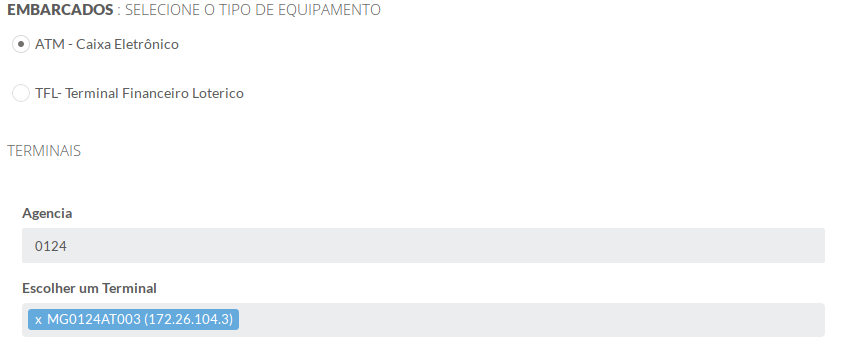
\includegraphics[width=17.029cm,height=7.22cm]{figuras/RATCETECATMSTFLS051718v2-img002.png}
        \end{center}


        \begin{center}
        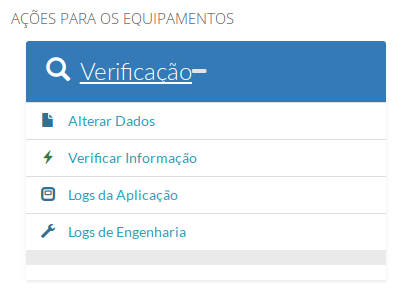
\includegraphics[width=10.82cm,height=7.777cm]{figuras/RATCETECATMSTFLS051718v2-img003.png}
        \end{center}
{\color{black}
    \ \ \ \ Dessa forma, ao solicitar a verifica\c{c}\~ao de informa\c{c}\~oes, o servidor ir\'a recuperar os dados
        atrav\'es do servi\c{c}o ssh na m\'aquina. Ele ir\'a levantar todas as informa\c{c}\~oes e ir\'a apresentar as suas
        informa\c{c}\~oes ao usu\'ario. As informa\c{c}\~oes coletadas ser\~ao as seguintes:}


        \bigskip

{\color{black}
    \ \ }

    \begin{center}
    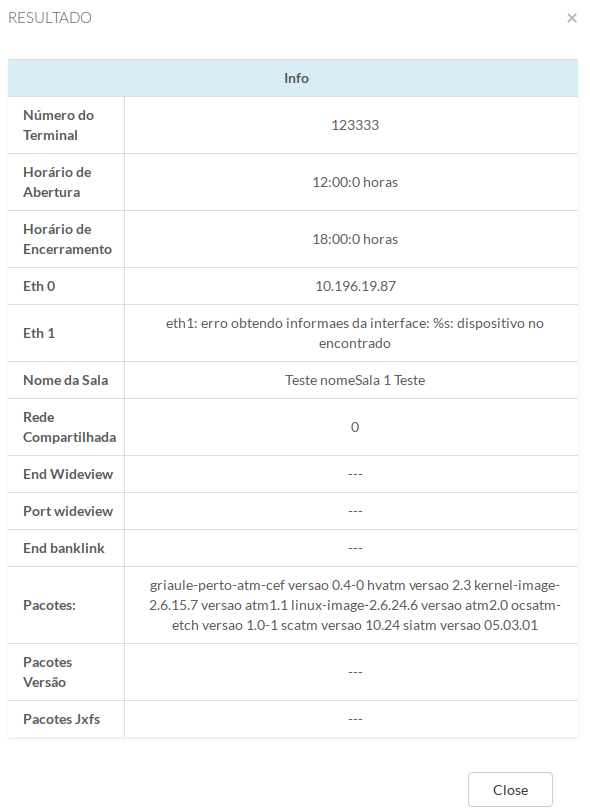
\includegraphics[width=13.936cm,height=19.131cm]{figuras/RATCETECATMSTFLS051718v2-img004.png}
    \end{center}

    \bigskip


    \bigskip

    \subsection[\ \ Altera\c{c}\~ao de Dados]{\ \ Altera\c{c}\~ao de Dados}
{\color{black}
    \ \ Para a aplica\c{c}\~ao de altera\c{c}\~ao de dados, no momento, \'e apresentado um formul\'ario que possibilita a
        altera\c{c}\~ao de dados j\'a existentes. Para aplicar uma altera\c{c}\~ao de dados, \'e necess\'ario escolher a
        m\'aquina que receber\'a a mudan\c{c}a.}

{\color{black}
    \ \ Ao escolher o terminal, \'e poss\'ivel selecionar a op\c{c}\~ao para executar a altera\c{c}\~ao, como visto na
        representa\c{c}\~ao a seguir:}

{\color{black}
    \ \ \ \ Sendo selecionada a op\c{c}\~ao, ser\'a apresentado ao usu\'ario o formul\'ario, como dito acima:}

    \begin{center}
    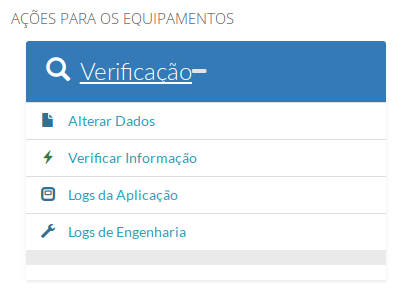
\includegraphics[width=10.82cm,height=7.777cm]{figuras/RATCETECATMSTFLS051718v2-img005.png}
    \end{center}

    \bigskip

{\color{black}
    \ \ Ap\'os o preenchimento do formul\'ario com as devidas informa\c{c}\~oes, estas ser\~ao enviadas para o servidor e
        aplicadas na respectiva m\'aquina. Assim, ir\'a ser criada uma barra de carregamento na parte inferior do site que
        apontar\'a o status atual da tarefa, sendo em progresso ou conclu\'ido. }

        \begin{center}
        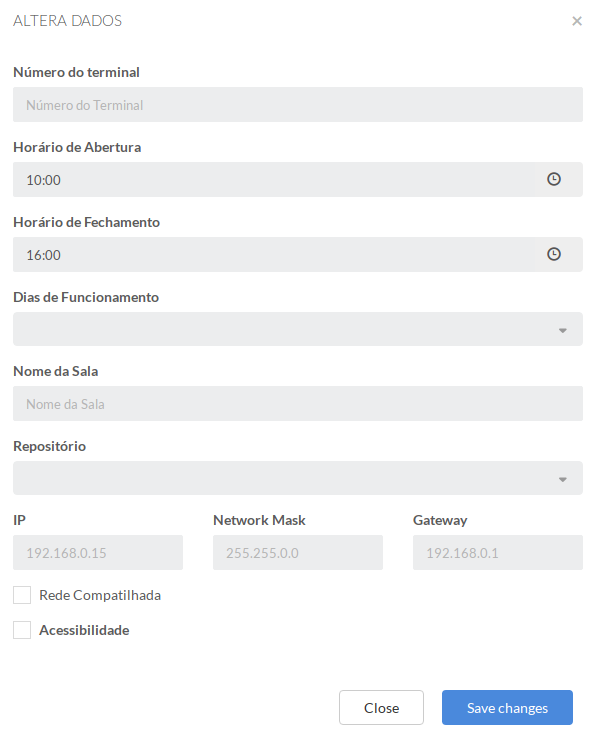
\includegraphics[width=15.279cm,height=18.83cm]{figuras/RATCETECATMSTFLS051718v2-img006.png}
        \end{center}

        \bigskip


        \bigskip


        \bigskip

{\color{black}
    \ \ Ao ter a tarefa finalizada, ser\'a apresentado o status de conclu\'ido e de visualiza\c{c}\~ao dos logs.}

    \begin{center}
    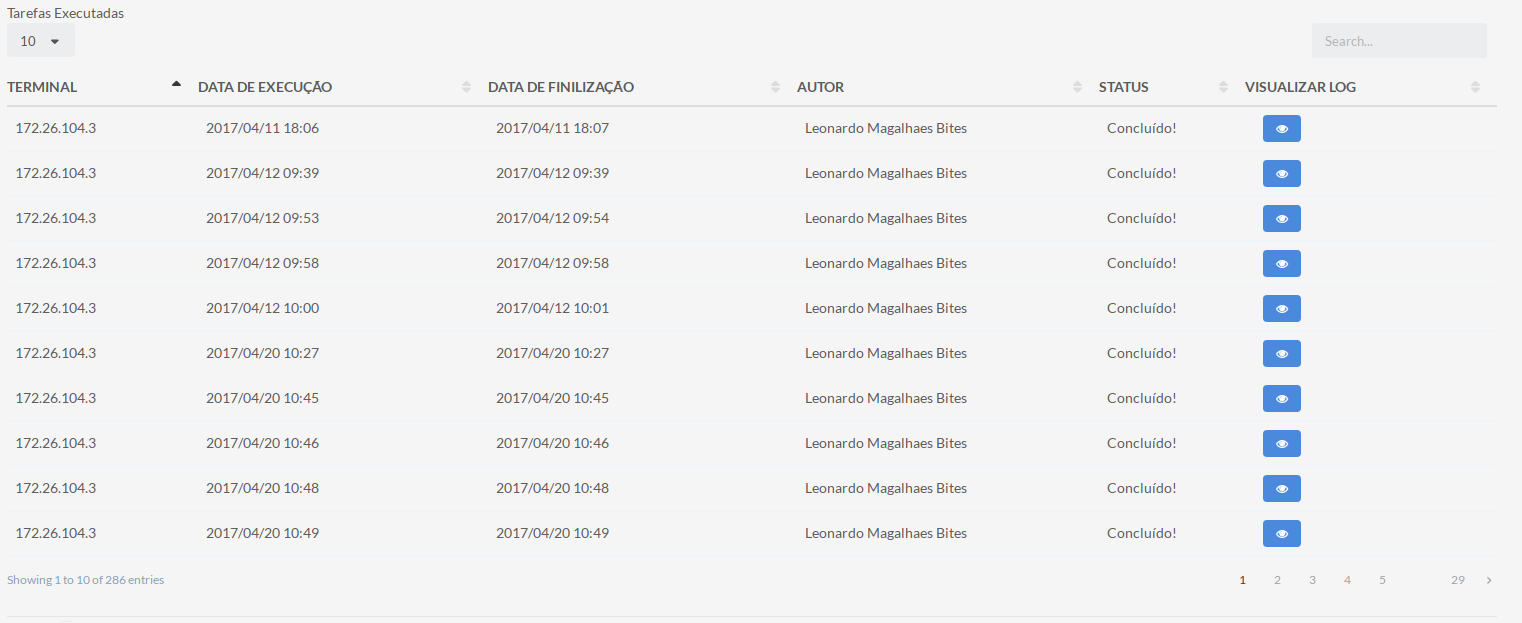
\includegraphics[width=17.029cm,height=6.969cm]{figuras/RATCETECATMSTFLS051718v2-img007.png}
    \end{center}

    \bigskip

    \subsection{Salvar Logs}
{\color{black}
    \ \ A funcionalidade de salvar log tem como objetivo principal recuperar dois tipos de logs dos terminais. O primeiro
        deles s\~ao os logs da aplica\c{c}\~ao SIMMA, sendo que o segundo s\~ao os logs de engenharia. }

{\color{black}
    \ \ Ap\'os escolher o terminal, que ter\'a o log recolhido, existem duas op\c{c}\~oes para a recupera\c{c}\~ao dos logs,
        como dito a pouco. Estas est\~ao dispostas como exemplificado na tela a seguir:}


        \bigskip

{\color{black}
    \ \ Ao solicitar uma das duas aplica\c{c}\~oes de logs, ser\'a enviada uma solicita\c{c}\~ao para as m\'aquinas, que
        ir\~ao armazenar os dados e enviar para o site. Assim, ser\'a indicado na barra de status, mencionada a pouco, que foi
        finalizada a tarefa com sinal de conclu\'ida. O usu\'ario dever\'a selecionar a op\c{c}\~ao de visualizar log e, logo
        em seguir, baixar o log. }

        \begin{center}
        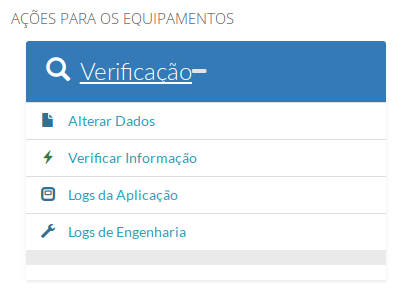
\includegraphics[width=10.82cm,height=7.777cm]{figuras/RATCETECATMSTFLS051718v2-img008.png}
        \end{center}

        \bigskip

        \subsection{Manuten\c{c}\~ao}
{\color{black}
    \ \ A manuten\c{c}\~ao permite que os terminais tenham manuten\c{c}\~oes pr\'e definidas. Estas podem ser aplicadas em
        v\'arios terminais ao mesmo tempo. \ Estes terminais devem ser escolhidos e assim, podem ser abordadas as
        manuten\c{c}\~oes, que est\~ao dispon\'iveis de acordo com a imagem do servidor a seguir:}


        \bigskip

        \section[Aspectos T\'ecnicos]{Aspectos T\'ecnicos}
        \begin{center}
        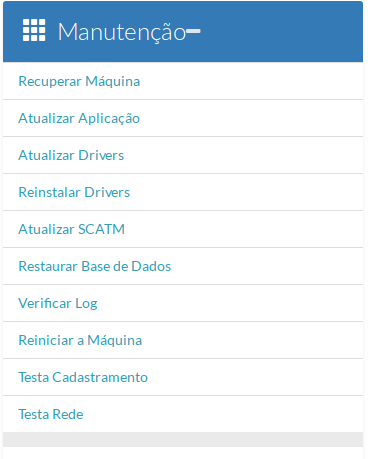
\includegraphics[width=9.793cm,height=12.143cm]{figuras/RATCETECATMSTFLS051718v2-img009.png}
        \end{center}
{\color{black}
    \ \ A seguir ser\~ao apresentados os procedimentos sistem\'aticos, que foram implementados para possibilitar o
        cumprimento dos requisitos desejados pelo cliente. Os cap\'itulos a seguir ser\~ao divididos bem como a arquitetura do
        software. O primeiro cap\'itulo ir\'a apresentar a parte de apresenta\c{c}\~ao, bem como HTML, CSS e JS. O segundo
        cap\'itulo apresentar\'a as views, que fazem e exercem o controle dos procedimentos solicitados ao servidor. Por fim,
        ser\~ao apresentados os procedimentos de implementa\c{c}\~ao nas modelos e scripts de execu\c{c}\~ao. }


        \subsection[Camada de Apresenta\c{c}\~ao]{Camada de Apresenta\c{c}\~ao}
{\color{black}
    A seguir ser\~ao apresentados os c\'odigos procedurais de apresenta\c{c}\~ao do site. O primeiro apresentado ser\'a a
        tela de index.html da tela de manuten\c{c}\~ao.}

{\ttfamily\color[rgb]{0.10980392,0.10980392,0.10980392}
    \{\% extends 'base.html' \%\}}

{\ttfamily\color[rgb]{0.10980392,0.10980392,0.10980392}
    \{\% if current\_user.is\_authenticated \%\}}


    \bigskip

{\ttfamily\color[rgb]{0.10980392,0.10980392,0.10980392}
    \{\% else \%\}}

{\ttfamily\color[rgb]{0.10980392,0.10980392,0.10980392}
    \ \ \ \ \{\% block login\%\}}


    \bigskip

{\ttfamily\color[rgb]{0.10980392,0.10980392,0.10980392}
    \ \ \ \ \{\% endblock \%\}}

{\ttfamily\color[rgb]{0.10980392,0.10980392,0.10980392}
    \{\% endif \%\}}


    \bigskip

{\ttfamily\color[rgb]{0.10980392,0.10980392,0.10980392}
    \{\% block container \%\}}


    \bigskip

{\ttfamily\color[rgb]{0.10980392,0.10980392,0.10980392}
    \ \ \ \ {\textless}style type={\textquotedbl}text/css{\textquotedbl}
    media={\textquotedbl}screen{\textquotedbl}{\textgreater}}

{\ttfamily\color[rgb]{0.10980392,0.10980392,0.10980392}
    body\{margin-top:50px;\}}

{\ttfamily\color[rgb]{0.10980392,0.10980392,0.10980392}
    .glyphicon \{ margin-right:10px; \}}

{\ttfamily\color[rgb]{0.10980392,0.10980392,0.10980392}
    .panel-body \{ padding:0px; \}}

{\ttfamily\color[rgb]{0.10980392,0.10980392,0.10980392}
    .panel-body table tr td \{ padding-left: 15px \}}

{\ttfamily\color[rgb]{0.10980392,0.10980392,0.10980392}
    .panel-body .table \{margin-bottom: 0px; \}}

{\ttfamily\color[rgb]{0.10980392,0.10980392,0.10980392}
    \ \ \ \ .clockpicker-popover \{}

{\ttfamily\color[rgb]{0.10980392,0.10980392,0.10980392}
    \ \ \ \ \ \ \ \ z-index: 999999 !important;}

{\ttfamily\color[rgb]{0.10980392,0.10980392,0.10980392}
    \ \ \ \ \}}

{\ttfamily\color[rgb]{0.10980392,0.10980392,0.10980392}
    \ \ \ \ {\textless}/style{\textgreater}}


    \bigskip

{\ttfamily\color[rgb]{0.10980392,0.10980392,0.10980392}
    \ \ \ \ \{\% block extracss \%\}}

{\ttfamily\color[rgb]{0.10980392,0.10980392,0.10980392}
    \ \ \ \ \ \ \ \ {\textless}link href={\textquotedbl}/static/css/get\_machines.css{\textquotedbl}
    rel={\textquotedbl}stylesheet{\textquotedbl}{\textgreater} {\textless}!-{}- MANDATORY -{}-{\textgreater}}

{\ttfamily\color[rgb]{0.10980392,0.10980392,0.10980392}
    \ \ \ \ \ \ \ \ {\textless}link
        href={\textquotedbl}/static/plugins\_new/clockpicker-gh-pages/src/standalone.css{\textquotedbl}
    rel={\textquotedbl}stylesheet{\textquotedbl}{\textgreater} {\textless}!-{}- MANDATORY -{}-{\textgreater}}

{\ttfamily\color[rgb]{0.10980392,0.10980392,0.10980392}
    \ \ \ \ \ \ \ \ {\textless}link
        href={\textquotedbl}/static/plugins\_new/clockpicker-gh-pages/src/clockpicker.css{\textquotedbl}
    rel={\textquotedbl}stylesheet{\textquotedbl}{\textgreater} {\textless}!-{}- MANDATORY -{}-{\textgreater}}

{\ttfamily\color[rgb]{0.10980392,0.10980392,0.10980392}
    \ \ \ \ \ \ \ \ {\textless}script type={\textquotedbl}text/javascript{\textquotedbl}
    src={\textquotedbl}{\textquotedbl}{\textgreater}{\textless}/script{\textgreater}}

{\ttfamily\color[rgb]{0.10980392,0.10980392,0.10980392}
    \ \ \ \ \{\% endblock \%\}}

{\ttfamily\color[rgb]{0.10980392,0.10980392,0.10980392}
    \ \ \ \ \{\% include 'manutencao/modal\_info.html' \%\}}

{\ttfamily\color[rgb]{0.10980392,0.10980392,0.10980392}
    \ \ \ \ \{\% include 'manutencao/modal\_change.html' \%\}}

{\ttfamily\color[rgb]{0.10980392,0.10980392,0.10980392}
    \ \ \ \ {\textless}h1{\textgreater}Manuten\c{c}\~ao Embarcados{\textless}/h1{\textgreater} \ \ \ }

{\ttfamily\color[rgb]{0.10980392,0.10980392,0.10980392}
    \ \ \ \ {\textless}div class={\textquotedbl}panel panel-default{\textquotedbl}{\textgreater}}

{\ttfamily\color[rgb]{0.10980392,0.10980392,0.10980392}
    \ \ \ \ \ \ \ \ {\textless}div class={\textquotedbl}panel-header{\textquotedbl}{\textgreater}}

{\ttfamily\color[rgb]{0.10980392,0.10980392,0.10980392}
    \ \ \ \ \ \ \ \ \ \ \ \ {\textless}h3{\textgreater}{\textless}i class={\textquotedbl}fa
        fa-gears{\textquotedbl}{\textgreater}{\textless}/i{\textgreater} Manuten\c{c}\~ao
        {\textless}strong{\textgreater}Remota{\textless}/strong{\textgreater}{\textless}/h3{\textgreater}}

{\ttfamily\color[rgb]{0.10980392,0.10980392,0.10980392}
    \ \ \ \ \ \ \ \ {\textless}/div{\textgreater}}

{\ttfamily\color[rgb]{0.10980392,0.10980392,0.10980392}
    \ \ \ \ \ \ \ \ {\textless}div class={\textquotedbl}panel-content{\textquotedbl}{\textgreater}}

{\ttfamily\color[rgb]{0.10980392,0.10980392,0.10980392}
    \ \ \ \ \ \ \ \ \ \ \ \ {\textless}div class={\textquotedbl}row{\textquotedbl}{\textgreater}}

{\ttfamily\color[rgb]{0.10980392,0.10980392,0.10980392}
    \ \ \ \ \ \ \ \ \ \ \ \ \ \ \ \ {\textless}div class={\textquotedbl}col-sm-7{\textquotedbl}{\textgreater}}

{\ttfamily\color[rgb]{0.10980392,0.10980392,0.10980392}
    \ \ \ \ \ \ \ \ \ \ \ \ \ \ \ \ \ \ \ \ {\textless}h3{\textgreater}{\textless}strong{\textgreater}Embarcados{\textless}/strong{\textgreater}
    : Selecione o tipo de equipamento{\textless}/h3{\textgreater}}


    \bigskip

{\ttfamily\color[rgb]{0.10980392,0.10980392,0.10980392}
    \ \ \ \ \ \ \ \ \ \ \ \ \ \ \ \ \ \ \ \ {\textless}form
        \ class={\textquotedbl}form-horizontal{\textquotedbl}{\textgreater}}

{\ttfamily\color[rgb]{0.10980392,0.10980392,0.10980392}
    \ \ \ \ \ \ \ \ \ \ \ \ \ \ \ \ \ \ \ \ \ \ \ \ {\textless}div
        class={\textquotedbl}form-group{\textquotedbl}{\textgreater}}

{\ttfamily\color[rgb]{0.10980392,0.10980392,0.10980392}
    \ \ \ \ \ \ \ \ \ \ \ \ \ \ \ \ \ \ \ \ \ \ \ \ \ \ \ \ {\textless}div
        class={\textquotedbl}radio{\textquotedbl}{\textgreater}}

{\ttfamily\color[rgb]{0.10980392,0.10980392,0.10980392}
    \ \ \ \ \ \ \ \ \ \ \ \ \ \ \ \ \ \ \ \ \ \ \ \ \ \ \ \ \ \ \ \ {\textless}label{\textgreater}{\textless}input
        \ \ checked id={\textquotedbl}Tipo\_de\_imagem{\textquotedbl} name={\textquotedbl}Tipo\_de\_imagem{\textquotedbl}
    value={\textquotedbl}ATM{\textquotedbl} type={\textquotedbl}radio{\textquotedbl}{\textgreater}ATM - Caixa
        Eletr\^onico{\textless}/label{\textgreater}}

{\ttfamily\color[rgb]{0.10980392,0.10980392,0.10980392}
    \ \ \ \ \ \ \ \ \ \ \ \ \ \ \ \ \ \ \ \ \ \ \ \ \ \ \ \ {\textless}/div{\textgreater}}

{\ttfamily\color[rgb]{0.10980392,0.10980392,0.10980392}
    \ \ \ \ \ \ \ \ \ \ \ \ \ \ \ \ \ \ \ \ \ \ \ \ {\textless}/div{\textgreater}}

{\ttfamily\color[rgb]{0.10980392,0.10980392,0.10980392}
    \ \ \ \ \ \ \ \ \ \ \ \ \ \ \ \ \ \ \ \ \ \ \ \ {\textless}div
        class={\textquotedbl}form-group{\textquotedbl}{\textgreater}}

{\ttfamily\color[rgb]{0.10980392,0.10980392,0.10980392}
    \ \ \ \ \ \ \ \ \ \ \ \ \ \ \ \ \ \ \ \ \ \ \ \ \ \ \ \ {\textless}div
        class={\textquotedbl}radio{\textquotedbl}{\textgreater}}

{\ttfamily\color[rgb]{0.10980392,0.10980392,0.10980392}
    \ \ \ \ \ \ \ \ \ \ \ \ \ \ \ \ \ \ \ \ \ \ \ \ \ \ \ \ \ \ \ \ {\textless}label{\textgreater}{\textless}input
        id={\textquotedbl}Tipo\_de\_imagem{\textquotedbl} name={\textquotedbl}Tipo\_de\_imagem{\textquotedbl}
    value={\textquotedbl}TFL{\textquotedbl} type={\textquotedbl}radio{\textquotedbl}{\textgreater}TFL- Terminal Financeiro
        Loterico{\textless}/label{\textgreater}}

{\ttfamily\color[rgb]{0.10980392,0.10980392,0.10980392}
    \ \ \ \ \ \ \ \ \ \ \ \ \ \ \ \ \ \ \ \ \ \ \ \ \ \ \ \ {\textless}/div{\textgreater}}

{\ttfamily\color[rgb]{0.10980392,0.10980392,0.10980392}
    \ \ \ \ \ \ \ \ \ \ \ \ \ \ \ \ \ \ \ \ \ \ \ \ {\textless}/div{\textgreater}}


    \bigskip

{\ttfamily\color[rgb]{0.10980392,0.10980392,0.10980392}
    \ \ \ \ \ \ \ \ \ \ \ \ \ \ \ \ \ \ \ \ \ \ \ \ {\textless}div
        class={\textquotedbl}form-group{\textquotedbl}{\textgreater}}

{\ttfamily\color[rgb]{0.10980392,0.10980392,0.10980392}
    \ \ \ \ \ \ \ \ \ \ \ \ \ \ \ \ \ \ \ \ \ \ \ \ \ \ \ \ {\textless}div
        class={\textquotedbl}radio{\textquotedbl}{\textgreater}}

{\ttfamily\color[rgb]{0.10980392,0.10980392,0.10980392}
    \ \ \ \ \ \ \ \ \ \ \ \ \ \ \ \ \ \ \ \ \ \ \ \ \ \ \ \ \ \ \ \ {\textless}label{\textgreater}{\textless}input
        \ id={\textquotedbl}Tipo\_de\_imagem{\textquotedbl} name={\textquotedbl}Tipo\_de\_imagem{\textquotedbl}
    value={\textquotedbl}SIPNL{\textquotedbl} type={\textquotedbl}radio{\textquotedbl}{\textgreater}SIPNL - Toten e
        Thinclients{\textless}/label{\textgreater}}

{\ttfamily\color[rgb]{0.10980392,0.10980392,0.10980392}
    \ \ \ \ \ \ \ \ \ \ \ \ \ \ \ \ \ \ \ \ \ \ \ \ \ \ \ \ {\textless}/div{\textgreater}}

{\ttfamily\color[rgb]{0.10980392,0.10980392,0.10980392}
    \ \ \ \ \ \ \ \ \ \ \ \ \ \ \ \ \ \ \ \ \ \ \ \ {\textless}/div{\textgreater}}

{\ttfamily\color[rgb]{0.10980392,0.10980392,0.10980392}
    \ \ \ \ \ \ \ \ \ \ \ \ \ \ \ \ \ \ \ \ \ \ \ \ {\textless}input value='\{\{current\_user.username\}\}' type='hidden'
        id='username'{\textgreater}}

{\ttfamily\color[rgb]{0.10980392,0.10980392,0.10980392}
    \ \ \ \ \ \ \ \ \ \ \ \ \ \ \ \ \ \ \ \ \ \ \ \ {\textless}h3{\textgreater}Terminais{\textless}/h3{\textgreater}}

{\ttfamily\color[rgb]{0.10980392,0.10980392,0.10980392}
    \ \ \ \ \ \ \ \ \ \ \ \ \ \ \ \ \ \ \ \ \ \ \ \ {\textless}div
        class={\textquotedbl}form-group{\textquotedbl}{\textgreater} }

{\ttfamily\color[rgb]{0.10980392,0.10980392,0.10980392}
    \ \ \ \ \ \ \ \ \ \ \ \ \ \ \ \ \ \ \ \ \ \ \ \ {\textless}/div{\textgreater}}

{\ttfamily\color[rgb]{0.10980392,0.10980392,0.10980392}
    \ \ \ \ \ \ \ \ \ \ \ \ \ \ \ \ \ \ \ \ {\textless}/form{\textgreater}}

{\ttfamily\color[rgb]{0.10980392,0.10980392,0.10980392}
    \ \ \ \ \ \ \ \ \ \ \ \ \ \ \ \ \ \ \ \ {\textless}form method={\textquotedbl}post{\textquotedbl}{\textgreater}}

{\ttfamily\color[rgb]{0.10980392,0.10980392,0.10980392}
    \ \ \ \ \ \ \ \ \ \ \ \ \ \ \ \ \ \ \ \ \ \ \ \ {\textless}div
        class={\textquotedbl}modal-body{\textquotedbl}{\textgreater}}

{\ttfamily\color[rgb]{0.10980392,0.10980392,0.10980392}
    \ \ \ \ \ \ \ \ \ \ \ \ \ \ \ \ \ \ \ \ \ \ \ \ \ \ \ \ {\textless}div
        class={\textquotedbl}form-group{\textquotedbl}{\textgreater}}

{\ttfamily\color[rgb]{0.10980392,0.10980392,0.10980392}
    \ \ \ \ \ \ \ \ \ \ \ \ \ \ \ \ \ \ \ \ \ \ \ \ \ \ \ \ \ \ \ \ {\textless}label
        for={\textquotedbl}agencia{\textquotedbl}{\textgreater}Agencia{\textless}/label{\textgreater}}

{\ttfamily\color[rgb]{0.10980392,0.10980392,0.10980392}
    \ \ \ \ \ \ \ \ \ \ \ \ \ \ \ \ \ \ \ \ \ \ \ \ \ \ \ \ \ \ \ \ {\textless}input type={\textquotedbl}text{\textquotedbl}
    class={\textquotedbl}form-control{\textquotedbl} id={\textquotedbl}agencia{\textquotedbl}
    placeholder={\textquotedbl}Ag\^encia{\textquotedbl}{\textgreater}}

{\ttfamily\color[rgb]{0.10980392,0.10980392,0.10980392}
    \ \ \ \ \ \ \ \ \ \ \ \ \ \ \ \ \ \ \ \ \ \ \ \ \ \ \ \ {\textless}/div{\textgreater}}

{\ttfamily\color[rgb]{0.10980392,0.10980392,0.10980392}
    \ \ \ \ \ \ \ \ \ \ \ \ \ \ \ \ \ \ \ \ \ \ \ \ \ \ \ \ {\textless}div
        class={\textquotedbl}form-group{\textquotedbl}{\textgreater}}

{\ttfamily\color[rgb]{0.10980392,0.10980392,0.10980392}
    \ \ \ \ \ \ \ \ \ \ \ \ \ \ \ \ \ \ \ \ \ \ \ \ \ \ \ \ \ \ \ \ {\textless}label{\textgreater}Escolher um
        Terminal{\textless}/label{\textgreater}}

{\ttfamily\color[rgb]{0.10980392,0.10980392,0.10980392}
    \ \ \ \ \ \ \ \ \ \ \ \ \ \ \ \ \ \ \ \ \ \ \ \ \ \ \ \ \ \ \ \ {\textless}select id='terminalselect' multiple required
        class={\textquotedbl}form-control select2{\textquotedbl} name={\textquotedbl}terminal{\textquotedbl}
    style={\textquotedbl}width: 100\%;{\textquotedbl}{\textgreater}}

{\ttfamily\color[rgb]{0.10980392,0.10980392,0.10980392}
    \ \ \ \ \ \ \ \ \ \ \ \ \ \ \ \ \ \ \ \ \ \ \ \ \ \ \ \ \ \ \ \ \ \ \ \ \{\% for machine in machines \%\}}

{\ttfamily\color[rgb]{0.10980392,0.10980392,0.10980392}
    \ \ \ \ \ \ \ \ \ \ \ \ \ \ \ \ \ \ \ \ \ \ \ \ \ \ \ \ \ \ \ \ \ \ \ \ \ \ \ \ {\textless}option
        value={\textquotedbl}\{\{ machine.nome \}\}{\textquotedbl}{\textgreater}\{\{ machine.nome \}\} (Serial: \{\{}

                {\ttfamily\color[rgb]{0.10980392,0.10980392,0.10980392}
                \ \ \ \ \ \ \ \ \ \ \ \ \ \ \ \ \ \ \ \ \ \ \ \ \ \ \ \ \ \ \ \ \ \ \ \ \ \ \ \ machine.serial\_number \}\})}

{\ttfamily\color[rgb]{0.10980392,0.10980392,0.10980392}
    \ \ \ \ \ \ \ \ \ \ \ \ \ \ \ \ \ \ \ \ \ \ \ \ \ \ \ \ \ \ \ \ \ \ \ \ \ \ \ \ {\textless}/option{\textgreater}}

{\ttfamily\color[rgb]{0.10980392,0.10980392,0.10980392}
    \ \ \ \ \ \ \ \ \ \ \ \ \ \ \ \ \ \ \ \ \ \ \ \ \ \ \ \ \ \ \ \ \ \ \ \ \{\% endfor \%\}}

{\ttfamily\color[rgb]{0.10980392,0.10980392,0.10980392}
    \ \ \ \ \ \ \ \ \ \ \ \ \ \ \ \ \ \ \ \ \ \ \ \ \ \ \ \ \ \ \ \ {\textless}/select{\textgreater}}

{\ttfamily\color[rgb]{0.10980392,0.10980392,0.10980392}
    \ \ \ \ \ \ \ \ \ \ \ \ \ \ \ \ \ \ \ \ \ \ \ \ \ \ \ \ {\textless}/div{\textgreater}}

{\ttfamily\color[rgb]{0.10980392,0.10980392,0.10980392}
    \ \ \ \ \ \ \ \ \ \ \ \ \ \ \ \ \ \ \ \ \ \ \ \ {\textless}/div{\textgreater}}

{\ttfamily\color[rgb]{0.10980392,0.10980392,0.10980392}
    \ \ \ \ \ \ \ \ \ \ \ \ \ \ \ \ \ \ \ \ {\textless}/form{\textgreater}}


    \bigskip

{\ttfamily\color[rgb]{0.10980392,0.10980392,0.10980392}
    \ \ \ \ \ \ \ \ \ \ \ \ \ \ \ \ {\textless}/div{\textgreater}}

{\ttfamily\color[rgb]{0.10980392,0.10980392,0.10980392}
    \ \ \ \ \ \ \ \ \ \ \ \ \ \ \ \ {\textless}div class='col-md-4 col-md-offset-1'{\textgreater}}


    \bigskip


    \bigskip

{\ttfamily\color[rgb]{0.10980392,0.10980392,0.10980392}
    \ \ \ \ \ \ \ \ \ \ \ \ \ \ \ \ \ \ \ \ {\textless}div class={\textquotedbl}container{\textquotedbl}{\textgreater}}

{\ttfamily\color[rgb]{0.10980392,0.10980392,0.10980392}
    \ \ \ \ \ \ \ \ \ \ \ \ \ \ \ \ \ \ \ \ \ \ \ \ {\textless}div class={\textquotedbl}row{\textquotedbl}{\textgreater}}

{\ttfamily\color[rgb]{0.10980392,0.10980392,0.10980392}
    \ \ \ \ \ \ \ \ \ \ \ \ \ \ \ \ \ \ \ \ \ \ \ \ \ \ \ \ {\textless}h3{\textgreater} \ \ \ A\c{c}\~oes para os
        equipamentos{\textless}/h3{\textgreater}}

{\ttfamily\color[rgb]{0.10980392,0.10980392,0.10980392}
    \ \ \ \ \ \ \ \ \ \ \ \ \ \ \ \ \ \ \ \ \ \ \ \ \ \ \ \ {\textless}div class={\textquotedbl}col-sm-4
        col-md-4{\textquotedbl}{\textgreater}}

{\ttfamily\color[rgb]{0.10980392,0.10980392,0.10980392}
    \ \ \ \ \ \ \ \ \ \ \ \ \ \ \ \ \ \ \ \ \ \ \ \ \ \ \ \ \ \ \ \ \{\% include 'manutencao/accordion.html' \%\}}

{\ttfamily\color[rgb]{0.10980392,0.10980392,0.10980392}
    \ \ \ \ \ \ \ \ \ \ \ \ \ \ \ \ \ \ \ \ \ \ \ \ \ \ \ \ {\textless}/div{\textgreater}}

{\ttfamily\color[rgb]{0.10980392,0.10980392,0.10980392}
    \ \ \ \ \ \ \ \ \ \ \ \ \ \ \ \ \ \ \ \ \ \ \ \ {\textless}/div{\textgreater}}

{\ttfamily\color[rgb]{0.10980392,0.10980392,0.10980392}
    \ \ \ \ \ \ \ \ \ \ \ \ \ \ \ \ \ \ \ \ {\textless}/div{\textgreater}}

{\ttfamily\color[rgb]{0.10980392,0.10980392,0.10980392}
    \ \ \ \ \ \ \ \ \ \ \ \ \ \ \ \ {\textless}/div{\textgreater}}

{\ttfamily\color[rgb]{0.10980392,0.10980392,0.10980392}
    \ \ \ \ \ \ \ \ \ \ \ \ {\textless}/div{\textgreater}}

{\ttfamily\color[rgb]{0.10980392,0.10980392,0.10980392}
    \ \ \ \ \ \ \ \ {\textless}/div{\textgreater}}

{\ttfamily\color[rgb]{0.10980392,0.10980392,0.10980392}
    \ \ \ \ {\textless}/div{\textgreater}}

{\ttfamily\color[rgb]{0.10980392,0.10980392,0.10980392}
    \ \ \ \ {\textless}div class={\textquotedbl}box green-box{\textquotedbl}{\textgreater}}

{\ttfamily\color[rgb]{0.10980392,0.10980392,0.10980392}
    \ \ \ \ \ \ \ \ {\textless}div class={\textquotedbl}box-header{\textquotedbl}{\textgreater}Tarefas
        Executadas{\textless}/div{\textgreater}}

{\ttfamily\color[rgb]{0.10980392,0.10980392,0.10980392}
    \ \ \ \ \ \ \ \ {\textless}div class={\textquotedbl}box-body{\textquotedbl}{\textgreater}}

{\ttfamily\color[rgb]{0.10980392,0.10980392,0.10980392}
    \ \ \ \ \ \ \ \ \ \ \ \ {\textless}table id={\textquotedbl}task-table{\textquotedbl} class={\textquotedbl}table
        table-hover table-dynamic{\textquotedbl}{\textgreater}}

{\ttfamily\color[rgb]{0.10980392,0.10980392,0.10980392}
    \ \ \ \ \ \ \ \ \ \ \ \ \ \ \ \ {\textless}thead{\textgreater}}

{\ttfamily\color[rgb]{0.10980392,0.10980392,0.10980392}
    \ \ \ \ \ \ \ \ \ \ \ \ \ \ \ \ \ \ \ \ {\textless}tr{\textgreater}}

{\ttfamily\color[rgb]{0.10980392,0.10980392,0.10980392}
    \ \ \ \ \ \ \ \ \ \ \ \ \ \ \ \ \ \ \ \ \ \ \ \ {\textless}th{\textgreater}Terminal{\textless}/th{\textgreater}}

{\ttfamily\color[rgb]{0.10980392,0.10980392,0.10980392}
    \ \ \ \ \ \ \ \ \ \ \ \ \ \ \ \ \ \ \ \ \ \ \ \ {\textless}th{\textgreater}Data de
        Execu\c{c}\~ao{\textless}/th{\textgreater}}

{\ttfamily\color[rgb]{0.10980392,0.10980392,0.10980392}
    \ \ \ \ \ \ \ \ \ \ \ \ \ \ \ \ \ \ \ \ \ \ \ \ {\textless}th{\textgreater}Data de
        Finiliza\c{c}\~ao{\textless}/th{\textgreater}}

{\ttfamily\color[rgb]{0.10980392,0.10980392,0.10980392}
    \ \ \ \ \ \ \ \ \ \ \ \ \ \ \ \ \ \ \ \ \ \ \ \ {\textless}th{\textgreater}Autor{\textless}/th{\textgreater}}

{\ttfamily\color[rgb]{0.10980392,0.10980392,0.10980392}
    \ \ \ \ \ \ \ \ \ \ \ \ \ \ \ \ \ \ \ \ \ \ \ \ {\textless}th{\textgreater}Status{\textless}/th{\textgreater}}

{\ttfamily\color[rgb]{0.10980392,0.10980392,0.10980392}
    \ \ \ \ \ \ \ \ \ \ \ \ \ \ \ \ \ \ \ \ \ \ \ \ {\textless}th{\textgreater}Visualizar Log{\textless}/th{\textgreater}}

{\ttfamily\color[rgb]{0.10980392,0.10980392,0.10980392}
    \ \ \ \ \ \ \ \ \ \ \ \ \ \ \ \ \ \ \ \ {\textless}/tr{\textgreater}}

{\ttfamily\color[rgb]{0.10980392,0.10980392,0.10980392}
    \ \ \ \ \ \ \ \ \ \ \ \ \ \ \ \ {\textless}/thead{\textgreater}}

{\ttfamily\color[rgb]{0.10980392,0.10980392,0.10980392}
    \ \ \ \ \ \ \ \ \ \ \ \ \ \ \ \ {\textless}tbody id='table-body'{\textgreater}}

{\ttfamily\color[rgb]{0.10980392,0.10980392,0.10980392}
    \ \ \ \ \ \ \ \ \ \ \ \ \ \ \ \ \ \ \ \ \{\% for imagem in historico \%\}}

{\ttfamily\color[rgb]{0.10980392,0.10980392,0.10980392}
    \ \ \ \ \ \ \ \ \ \ \ \ \ \ \ \ \ \ \ \ \ \ \ \ {\textless}tr{\textgreater}}

{\ttfamily\color[rgb]{0.10980392,0.10980392,0.10980392}
    \ \ \ \ \ \ \ \ \ \ \ \ \ \ \ \ \ \ \ \ \ \ \ \ \ \ \ \ {\textless}td{\textgreater}\{\{
        imagem.tipo\}\}{\textless}/td{\textgreater}}

{\ttfamily\color[rgb]{0.10980392,0.10980392,0.10980392}
    \ \ \ \ \ \ \ \ \ \ \ \ \ \ \ \ \ \ \ \ \ \ \ \ \ \ \ \ {\textless}td{\textgreater}\{\{
        imagem.data\_execucao.strftime('\%Y/\%m/\%d \%H:\%M') \}\}{\textless}/td{\textgreater}}

{\ttfamily\color[rgb]{0.10980392,0.10980392,0.10980392}
    \ \ \ \ \ \ \ \ \ \ \ \ \ \ \ \ \ \ \ \ \ \ \ \ \ \ \ \ {\textless}td{\textgreater}\{\{
        imagem.data\_fim.strftime('\%Y/\%m/\%d \%H:\%M') \}\}{\textless}/td{\textgreater}}

{\ttfamily\color[rgb]{0.10980392,0.10980392,0.10980392}
    \ \ \ \ \ \ \ \ \ \ \ \ \ \ \ \ \ \ \ \ \ \ \ \ \ \ \ \ {\textless}td{\textgreater}\{\{imagem.usuario\}\}{\textless}/td{\textgreater}}

{\ttfamily\color[rgb]{0.10980392,0.10980392,0.10980392}
    \ \ \ \ \ \ \ \ \ \ \ \ \ \ \ \ \ \ \ \ \ \ \ \ \ \ \ \ {\textless}td{\textgreater}Conclu\'ido!
    {\textless}/td{\textgreater}}

{\ttfamily\color[rgb]{0.10980392,0.10980392,0.10980392}
    \ \ \ \ \ \ \ \ \ \ \ \ \ \ \ \ \ \ \ \ \ \ \ \ \ \ \ \ {\textless}td{\textgreater}}

{\ttfamily\color[rgb]{0.10980392,0.10980392,0.10980392}
    \ \ \ \ \ \ \ \ \ \ \ \ \ \ \ \ \ \ \ \ \ \ \ \ \ \ \ \ \ \ \ \ {\textless}p style={\textquotedbl}display:
        none;{\textquotedbl}{\textgreater}\{\{ imagem.id \}\}{\textless}/p{\textgreater}}

{\ttfamily\color[rgb]{0.10980392,0.10980392,0.10980392}
    \ \ \ \ \ \ \ \ \ \ \ \ \ \ \ \ \ \ \ \ \ \ \ \ \ \ \ \ \ \ \ \ {\textless}button
        onclick={\textquotedbl}manage\_logs(\$(this)){\textquotedbl} href={\textquotedbl}/log\_manutencao/\{\{ imagem.id
        \}\}{\textquotedbl} class={\textquotedbl}btn btn-sm btn-primary jenkins\_output
        showlog{\textquotedbl}{\textgreater}{\textless}i class={\textquotedbl}fa
        fa-eye{\textquotedbl}{\textgreater}{\textless}/i{\textgreater}{\textless}/button{\textgreater}}

{\ttfamily\color[rgb]{0.10980392,0.10980392,0.10980392}
    \ \ \ \ \ \ \ \ \ \ \ \ \ \ \ \ \ \ \ \ \ \ \ \ \ \ \ \ {\textless}/td{\textgreater}}

{\ttfamily\color[rgb]{0.10980392,0.10980392,0.10980392}
    \ \ \ \ \ \ \ \ \ \ \ \ \ \ \ \ \ \ \ \ \ \ \ \ {\textless}/tr{\textgreater}}

{\ttfamily\color[rgb]{0.10980392,0.10980392,0.10980392}
    \ \ \ \ \ \ \ \ \ \ \ \ \ \ \ \ \ \ \ \ \{\% endfor \%\}}

{\ttfamily\color[rgb]{0.10980392,0.10980392,0.10980392}
    \ \ \ \ \ \ \ \ \ \ \ \ \ \ \ \ {\textless}/tbody{\textgreater}}

{\ttfamily\color[rgb]{0.10980392,0.10980392,0.10980392}
    \ \ \ \ \ \ \ \ \ \ \ \ {\textless}/table{\textgreater}}

{\ttfamily\color[rgb]{0.10980392,0.10980392,0.10980392}
    \ \ \ \ \ \ \ \ {\textless}/div{\textgreater}}

{\ttfamily\color[rgb]{0.10980392,0.10980392,0.10980392}
    \ \ \ \ {\textless}/div{\textgreater}}

{\ttfamily\color[rgb]{0.10980392,0.10980392,0.10980392}
    \ \ \ \ {\textless}!-{}- scripts js -{}-{\textgreater}}

{\ttfamily\color[rgb]{0.10980392,0.10980392,0.10980392}
    \ \ \ \ \{\% block extrascripts \%\}}

{\ttfamily\color[rgb]{0.10980392,0.10980392,0.10980392}
    \ \ \ \ \ \ \ \ {\textless}script type={\textquotedbl}text/javascript{\textquotedbl}
    src={\textquotedbl}/static/js/signature\_create.min.js{\textquotedbl}{\textgreater}{\textless}/script{\textgreater}}

{\ttfamily\color[rgb]{0.10980392,0.10980392,0.10980392}
    \ \ \ \ \ \ \ \ {\textless}script
        src={\textquotedbl}//cdnjs.cloudflare.com/ajax/libs/nanobar/0.2.1/nanobar.min.js{\textquotedbl}{\textgreater}{\textless}/script{\textgreater}}

{\ttfamily\color[rgb]{0.10980392,0.10980392,0.10980392}
    \ \ \ \ \ \ \ \ {\textless}script type={\textquotedbl}text/javascript{\textquotedbl}
    src={\textquotedbl}/static/js/widget.js{\textquotedbl}{\textgreater}{\textless}/script{\textgreater}}

{\ttfamily\color[rgb]{0.10980392,0.10980392,0.10980392}
    \ \ \ \ \ \ \ \ {\textless}script type={\textquotedbl}text/javascript{\textquotedbl}
    src={\textquotedbl}/static/js/manutencao.js{\textquotedbl}{\textgreater}{\textless}/script{\textgreater}}

{\ttfamily\color[rgb]{0.10980392,0.10980392,0.10980392}
    \ \ \ \ \ \ \ \ {\textless}script type={\textquotedbl}text/javascript{\textquotedbl}
    src={\textquotedbl}/static/js/notifications.js{\textquotedbl}{\textgreater}{\textless}/script{\textgreater}}

{\ttfamily\color[rgb]{0.10980392,0.10980392,0.10980392}
    \ \ \ \ \ \ \ \ {\textless}script type={\textquotedbl}text/javascript{\textquotedbl}
    src={\textquotedbl}/static/js/get\_machines.js{\textquotedbl}{\textgreater}{\textless}/script{\textgreater}}

{\ttfamily\color[rgb]{0.10980392,0.10980392,0.10980392}
    \ \ \ \ \ \ \ \ {\textless}script type='text/javascript'
        src={\textquotedbl}/static/plugins\_new/clockpicker-gh-pages/src/clockpicker.js{\textquotedbl}{\textgreater}
    {\textless}!-{}- MANDATORY -{}-{\textgreater}}

{\ttfamily\color[rgb]{0.10980392,0.10980392,0.10980392}
    {\textless}script type={\textquotedbl}text/javascript{\textquotedbl}{\textgreater}}

{\ttfamily\color[rgb]{0.10980392,0.10980392,0.10980392}
    \$('.clockpicker').clockpicker();}

{\ttfamily\color[rgb]{0.10980392,0.10980392,0.10980392}
    {\textless}/script{\textgreater}}

{\ttfamily\color[rgb]{0.10980392,0.10980392,0.10980392}
    {\textless}script type={\textquotedbl}text/javascript{\textquotedbl}{\textgreater}}

{\ttfamily\color[rgb]{0.10980392,0.10980392,0.10980392}
    var input = \$('\#single-input').clockpicker(\{}

            {\ttfamily\color[rgb]{0.10980392,0.10980392,0.10980392}
            \ \ \ \ placement: 'bottom',}

            {\ttfamily\color[rgb]{0.10980392,0.10980392,0.10980392}
            \ \ \ \ align: 'left',}

            {\ttfamily\color[rgb]{0.10980392,0.10980392,0.10980392}
            \ \ \ \ autoclose: true,}

            {\ttfamily\color[rgb]{0.10980392,0.10980392,0.10980392}
            \ \ \ \ {}'default': 'now'}

            {\ttfamily\color[rgb]{0.10980392,0.10980392,0.10980392}
            \});}


    \bigskip

{\ttfamily\color[rgb]{0.10980392,0.10980392,0.10980392}
    // Manually toggle to the minutes view}

{\ttfamily\color[rgb]{0.10980392,0.10980392,0.10980392}
    \$('\#check-minutes').click(function(e)\{}

            {\ttfamily\color[rgb]{0.10980392,0.10980392,0.10980392}
            \ \ \ \ // Have to stop propagation here}

            {\ttfamily\color[rgb]{0.10980392,0.10980392,0.10980392}
            \ \ \ \ e.stopPropagation();}

            {\ttfamily\color[rgb]{0.10980392,0.10980392,0.10980392}
            \ \ \ \ input.clockpicker('show')}

            {\ttfamily\color[rgb]{0.10980392,0.10980392,0.10980392}
            \ \ \ \ \ \ \ \ .clockpicker('toggleView', 'minutes');}

            {\ttfamily\color[rgb]{0.10980392,0.10980392,0.10980392}
            \});}

{\ttfamily\color[rgb]{0.10980392,0.10980392,0.10980392}
    {\textless}/script{\textgreater}}

{\ttfamily\color[rgb]{0.10980392,0.10980392,0.10980392}
    \ \ \ \ \{\% endblock \%\}}

{\ttfamily\color[rgb]{0.10980392,0.10980392,0.10980392}
    \{\% endblock \%\}}


    \bigskip

{\color{black}
    \ \ Agora ser\'a apresentado o accordion, que possui todas as informa\c{c}\~oes e op\c{c}\~oes de implanta\c{c}\~ao de
        dados.}

{\ttfamily\color[rgb]{0.10980392,0.10980392,0.10980392}
    {\textgreater} cat templates/manutencao/accordion.html }

{\ttfamily\color[rgb]{0.10980392,0.10980392,0.10980392}
    {\textless}div class={\textquotedbl}panel-group{\textquotedbl} id={\textquotedbl}accordion{\textquotedbl}{\textgreater}}

{\ttfamily\color[rgb]{0.10980392,0.10980392,0.10980392}
    \ \ \ \ {\textless}div class={\textquotedbl}panel panel-primary{\textquotedbl}{\textgreater}}

{\ttfamily\color[rgb]{0.10980392,0.10980392,0.10980392}
    \ \ \ \ \ \ \ \ {\textless}div class={\textquotedbl}panel-heading{\textquotedbl}{\textgreater}}

{\ttfamily\color[rgb]{0.10980392,0.10980392,0.10980392}
    \ \ \ \ \ \ \ \ \ \ \ \ {\textless}h4 class={\textquotedbl}panel-title{\textquotedbl}{\textgreater}}

{\ttfamily\color[rgb]{0.10980392,0.10980392,0.10980392}
    \ \ \ \ \ \ \ \ \ \ \ \ \ \ \ \ {\textless}a data-toggle={\textquotedbl}collapse{\textquotedbl}
    data-parent={\textquotedbl}\#accordion{\textquotedbl}
    href={\textquotedbl}\#collapseOne{\textquotedbl}{\textgreater}{\textless}span class={\textquotedbl}glyphicon
        glyphicon-folder-close{\textquotedbl}{\textgreater}}

{\ttfamily\color[rgb]{0.10980392,0.10980392,0.10980392}
    \ \ \ \ \ \ \ \ \ \ \ \ \ \ \ \ \ \ \ \ {\textless}/span{\textgreater}Verifica\c{c}\~ao{\textless}/a{\textgreater}}

{\ttfamily\color[rgb]{0.10980392,0.10980392,0.10980392}
    \ \ \ \ \ \ \ \ \ \ \ \ {\textless}/h4{\textgreater}}

{\ttfamily\color[rgb]{0.10980392,0.10980392,0.10980392}
    \ \ \ \ \ \ \ \ {\textless}/div{\textgreater}}

{\ttfamily\color[rgb]{0.10980392,0.10980392,0.10980392}
    \ \ \ \ \ \ \ \ {\textless}div id={\textquotedbl}collapseOne{\textquotedbl} class={\textquotedbl}panel-collapse
        collapse{\textquotedbl}{\textgreater}}

{\ttfamily\color[rgb]{0.10980392,0.10980392,0.10980392}
    \ \ \ \ \ \ \ \ \ \ \ \ {\textless}div class={\textquotedbl}panel-body{\textquotedbl}{\textgreater}}

{\ttfamily\color[rgb]{0.10980392,0.10980392,0.10980392}
    \ \ \ \ \ \ \ \ \ \ \ \ \ \ \ \ {\textless}table class={\textquotedbl}table{\textquotedbl}{\textgreater}}

{\ttfamily\color[rgb]{0.10980392,0.10980392,0.10980392}
    \ \ \ \ \ \ \ \ \ \ \ \ \ \ \ \ \ \ \ \ {\textless}tr{\textgreater}}

{\ttfamily\color[rgb]{0.10980392,0.10980392,0.10980392}
    \ \ \ \ \ \ \ \ \ \ \ \ \ \ \ \ \ \ \ \ \ \ \ \ {\textless}td{\textgreater}}

{\ttfamily\color[rgb]{0.10980392,0.10980392,0.10980392}
    \ \ \ \ \ \ \ \ \ \ \ \ \ \ \ \ \ \ \ \ \ \ \ \ \ \ \ \ {\textless}span class={\textquotedbl}glyphicon glyphicon-file
        text-info{\textquotedbl}{\textgreater}{\textless}/span{\textgreater}}

{\ttfamily\color[rgb]{0.10980392,0.10980392,0.10980392}
    \ \ \ \ \ \ \ \ \ \ \ \ \ \ \ \ \ \ \ \ \ \ \ \ \ \ \ \ {\textless}a data-toggle={\textquotedbl}modal{\textquotedbl}
    data-target={\textquotedbl}\#modal\_change{\textquotedbl} class='{}' href={\textquotedbl}\#{\textquotedbl}
    id='log\_simma' {\textgreater}Alterar Dados{\textless}/a{\textgreater}}

{\ttfamily\color[rgb]{0.10980392,0.10980392,0.10980392}
    \ \ \ \ \ \ \ \ \ \ \ \ \ \ \ \ \ \ \ \ \ \ \ \ {\textless}/td{\textgreater}}

{\ttfamily\color[rgb]{0.10980392,0.10980392,0.10980392}
    \ \ \ \ \ \ \ \ \ \ \ \ \ \ \ \ \ \ \ \ {\textless}/tr{\textgreater}}

{\ttfamily\color[rgb]{0.10980392,0.10980392,0.10980392}
    \ \ \ \ \ \ \ \ \ \ \ \ \ \ \ \ \ \ \ \ {\textless}tr{\textgreater}}

{\ttfamily\color[rgb]{0.10980392,0.10980392,0.10980392}
    \ \ \ \ \ \ \ \ \ \ \ \ \ \ \ \ \ \ \ \ \ \ \ \ {\textless}td{\textgreater}}

{\ttfamily\color[rgb]{0.10980392,0.10980392,0.10980392}
    \ \ \ \ \ \ \ \ \ \ \ \ \ \ \ \ \ \ \ \ \ \ \ \ \ \ \ \ {\textless}span class={\textquotedbl}glyphicon glyphicon-flash
        text-success{\textquotedbl}{\textgreater}{\textless}/span{\textgreater}}

{\ttfamily\color[rgb]{0.10980392,0.10980392,0.10980392}
    \ \ \ \ \ \ \ \ \ \ \ \ \ \ \ \ \ \ \ \ \ \ \ \ \ \ \ \ {\textless}a href={\textquotedbl}\#{\textquotedbl}
    class='button\_manutencao information' id='exec\_command'{\textgreater}Verificar
        Informa\c{c}\~ao{\textless}/a{\textgreater}}

{\ttfamily\color[rgb]{0.10980392,0.10980392,0.10980392}
    \ \ \ \ \ \ \ \ \ \ \ \ \ \ \ \ \ \ \ \ \ \ \ \ {\textless}/td{\textgreater}}

{\ttfamily\color[rgb]{0.10980392,0.10980392,0.10980392}
    \ \ \ \ \ \ \ \ \ \ \ \ \ \ \ \ \ \ \ \ {\textless}/tr{\textgreater}}

{\ttfamily\color[rgb]{0.10980392,0.10980392,0.10980392}
    \ \ \ \ \ \ \ \ \ \ \ \ \ \ \ \ \ \ \ \ {\textless}tr{\textgreater}}

{\ttfamily\color[rgb]{0.10980392,0.10980392,0.10980392}
    \ \ \ \ \ \ \ \ \ \ \ \ \ \ \ \ \ \ \ \ \ \ \ \ {\textless}td{\textgreater}}

{\ttfamily\color[rgb]{0.10980392,0.10980392,0.10980392}
    \ \ \ \ \ \ \ \ \ \ \ \ \ \ \ \ \ \ \ \ \ \ \ \ \ \ \ \ {\textless}span class={\textquotedbl}glyphicon
        glyphicon-modal-window text-info{\textquotedbl}{\textgreater}{\textless}/span{\textgreater}}

{\ttfamily\color[rgb]{0.10980392,0.10980392,0.10980392}
    \ \ \ \ \ \ \ \ \ \ \ \ \ \ \ \ \ \ \ \ \ \ \ \ \ \ \ \ {\textless}a class='button\_manutencao logs'
        href={\textquotedbl}\#{\textquotedbl} id='log\_simma' {\textgreater}Logs da Aplica\c{c}\~ao{\textless}/a{\textgreater}}

{\ttfamily\color[rgb]{0.10980392,0.10980392,0.10980392}
    \ \ \ \ \ \ \ \ \ \ \ \ \ \ \ \ \ \ \ \ \ \ \ \ {\textless}/td{\textgreater}}

{\ttfamily\color[rgb]{0.10980392,0.10980392,0.10980392}
    \ \ \ \ \ \ \ \ \ \ \ \ \ \ \ \ \ \ \ \ {\textless}/tr{\textgreater}}

{\ttfamily\color[rgb]{0.10980392,0.10980392,0.10980392}
    \ \ \ \ \ \ \ \ \ \ \ \ \ \ \ \ \ \ \ \ {\textless}tr{\textgreater}}

{\ttfamily\color[rgb]{0.10980392,0.10980392,0.10980392}
    \ \ \ \ \ \ \ \ \ \ \ \ \ \ \ \ \ \ \ \ \ \ \ \ {\textless}td{\textgreater}}

{\ttfamily\color[rgb]{0.10980392,0.10980392,0.10980392}
    \ \ \ \ \ \ \ \ \ \ \ \ \ \ \ \ \ \ \ \ \ \ \ \ \ \ \ \ {\textless}span class={\textquotedbl}glyphicon glyphicon-wrench
        text-info{\textquotedbl}{\textgreater}{\textless}/span{\textgreater}}

{\ttfamily\color[rgb]{0.10980392,0.10980392,0.10980392}
    \ \ \ \ \ \ \ \ \ \ \ \ \ \ \ \ \ \ \ \ \ \ \ \ \ \ \ \ {\textless}a class='button\_manutencao logs'
        href={\textquotedbl}\#{\textquotedbl} id='log\_eng' {\textgreater}Logs de Engenharia{\textless}/a{\textgreater}}

{\ttfamily\color[rgb]{0.10980392,0.10980392,0.10980392}
    \ \ \ \ \ \ \ \ \ \ \ \ \ \ \ \ \ \ \ \ \ \ \ \ {\textless}/td{\textgreater}}

{\ttfamily\color[rgb]{0.10980392,0.10980392,0.10980392}
    \ \ \ \ \ \ \ \ \ \ \ \ \ \ \ \ \ \ \ \ {\textless}/tr{\textgreater}}

{\ttfamily\color[rgb]{0.10980392,0.10980392,0.10980392}
    \ \ \ \ \ \ \ \ \ \ \ \ \ \ \ \ {\textless}/table{\textgreater}}

{\ttfamily\color[rgb]{0.10980392,0.10980392,0.10980392}
    \ \ \ \ \ \ \ \ \ \ \ \ {\textless}/div{\textgreater}}

{\ttfamily\color[rgb]{0.10980392,0.10980392,0.10980392}
    \ \ \ \ \ \ \ \ {\textless}/div{\textgreater}}

{\ttfamily\color[rgb]{0.10980392,0.10980392,0.10980392}
    \ \ \ \ {\textless}/div{\textgreater}}

{\ttfamily\color[rgb]{0.10980392,0.10980392,0.10980392}
    \ \ \ \ {\textless}div class={\textquotedbl}panel panel-primary{\textquotedbl}{\textgreater}}

{\ttfamily\color[rgb]{0.10980392,0.10980392,0.10980392}
    \ \ \ \ \ \ \ \ {\textless}div class={\textquotedbl}panel-heading{\textquotedbl}{\textgreater}}

{\ttfamily\color[rgb]{0.10980392,0.10980392,0.10980392}
    \ \ \ \ \ \ \ \ \ \ \ \ {\textless}h4 class={\textquotedbl}panel-title{\textquotedbl}{\textgreater}}

{\ttfamily\color[rgb]{0.10980392,0.10980392,0.10980392}
    \ \ \ \ \ \ \ \ \ \ \ \ \ \ \ \ {\textless}a data-toggle={\textquotedbl}collapse{\textquotedbl}
    data-parent={\textquotedbl}\#accordion{\textquotedbl}
    href={\textquotedbl}\#collapseTwo{\textquotedbl}{\textgreater}{\textless}span class={\textquotedbl}glyphicon
        glyphicon-th{\textquotedbl}{\textgreater}}

{\ttfamily\color[rgb]{0.10980392,0.10980392,0.10980392}
    \ \ \ \ \ \ \ \ \ \ \ \ \ \ \ \ \ \ \ \ {\textless}/span{\textgreater}Manuten\c{c}\~ao{\textless}/a{\textgreater}}

{\ttfamily\color[rgb]{0.10980392,0.10980392,0.10980392}
    \ \ \ \ \ \ \ \ \ \ \ \ {\textless}/h4{\textgreater}}

{\ttfamily\color[rgb]{0.10980392,0.10980392,0.10980392}
    \ \ \ \ \ \ \ \ {\textless}/div{\textgreater}}

{\ttfamily\color[rgb]{0.10980392,0.10980392,0.10980392}
    \ \ \ \ \ \ \ \ {\textless}div id={\textquotedbl}collapseTwo{\textquotedbl} class={\textquotedbl}panel-collapse
        collapse{\textquotedbl}{\textgreater}}

{\ttfamily\color[rgb]{0.10980392,0.10980392,0.10980392}
    \ \ \ \ \ \ \ \ \ \ \ \ {\textless}div class={\textquotedbl}panel-body{\textquotedbl}{\textgreater}}

{\ttfamily\color[rgb]{0.10980392,0.10980392,0.10980392}
    \ \ \ \ \ \ \ \ \ \ \ \ \ \ \ \ {\textless}table class={\textquotedbl}table{\textquotedbl}{\textgreater}}

{\ttfamily\color[rgb]{0.10980392,0.10980392,0.10980392}
    \ \ \ \ \ \ \ \ \ \ \ \ \ \ \ \ \ \ \ \ {\textless}tr{\textgreater}}

{\ttfamily\color[rgb]{0.10980392,0.10980392,0.10980392}
    \ \ \ \ \ \ \ \ \ \ \ \ \ \ \ \ \ \ \ \ \ \ \ \ {\textless}td{\textgreater}}

{\ttfamily\color[rgb]{0.10980392,0.10980392,0.10980392}
    \ \ \ \ \ \ \ \ \ \ \ \ \ \ \ \ \ \ \ \ \ \ \ \ \ \ \ \ {\textless}a class='button\_manutencao maintenance'
        href={\textquotedbl}\#{\textquotedbl} id='recovery' {\textgreater}Recuperar M\'aquina{\textless}/a{\textgreater}}

{\ttfamily\color[rgb]{0.10980392,0.10980392,0.10980392}
    \ \ \ \ \ \ \ \ \ \ \ \ \ \ \ \ \ \ \ \ \ \ \ \ {\textless}/td{\textgreater}}

{\ttfamily\color[rgb]{0.10980392,0.10980392,0.10980392}
    \ \ \ \ \ \ \ \ \ \ \ \ \ \ \ \ \ \ \ \ {\textless}/tr{\textgreater}}

{\ttfamily\color[rgb]{0.10980392,0.10980392,0.10980392}
    \ \ \ \ \ \ \ \ \ \ \ \ \ \ \ \ \ \ \ \ {\textless}tr{\textgreater}}

{\ttfamily\color[rgb]{0.10980392,0.10980392,0.10980392}
    \ \ \ \ \ \ \ \ \ \ \ \ \ \ \ \ \ \ \ \ \ \ \ \ {\textless}td{\textgreater}}

{\ttfamily\color[rgb]{0.10980392,0.10980392,0.10980392}
    \ \ \ \ \ \ \ \ \ \ \ \ \ \ \ \ \ \ \ \ \ \ \ \ \ \ \ \ {\textless}a class='button\_manutencao maintenance'
        href={\textquotedbl}\#{\textquotedbl} id='update\_application' {\textgreater}Atualizar
        Aplica\c{c}\~ao{\textless}/a{\textgreater}}

{\ttfamily\color[rgb]{0.10980392,0.10980392,0.10980392}
    \ \ \ \ \ \ \ \ \ \ \ \ \ \ \ \ \ \ \ \ \ \ \ \ {\textless}/td{\textgreater}}

{\ttfamily\color[rgb]{0.10980392,0.10980392,0.10980392}
    \ \ \ \ \ \ \ \ \ \ \ \ \ \ \ \ \ \ \ \ {\textless}/tr{\textgreater}}

{\ttfamily\color[rgb]{0.10980392,0.10980392,0.10980392}
    \ \ \ \ \ \ \ \ \ \ \ \ \ \ \ \ \ \ \ \ {\textless}tr{\textgreater}}

{\ttfamily\color[rgb]{0.10980392,0.10980392,0.10980392}
    \ \ \ \ \ \ \ \ \ \ \ \ \ \ \ \ \ \ \ \ \ \ \ \ {\textless}td{\textgreater}}

{\ttfamily\color[rgb]{0.10980392,0.10980392,0.10980392}
    \ \ \ \ \ \ \ \ \ \ \ \ \ \ \ \ \ \ \ \ \ \ \ \ \ \ \ \ {\textless}a class='button\_manutencao maintenance'
        href={\textquotedbl}\#{\textquotedbl} id='update\_drives' {\textgreater}Atualizar Drivers{\textless}/a{\textgreater}}

{\ttfamily\color[rgb]{0.10980392,0.10980392,0.10980392}
    \ \ \ \ \ \ \ \ \ \ \ \ \ \ \ \ \ \ \ \ \ \ \ \ {\textless}/td{\textgreater}}

{\ttfamily\color[rgb]{0.10980392,0.10980392,0.10980392}
    \ \ \ \ \ \ \ \ \ \ \ \ \ \ \ \ \ \ \ \ {\textless}/tr{\textgreater}}

{\ttfamily\color[rgb]{0.10980392,0.10980392,0.10980392}
    \ \ \ \ \ \ \ \ \ \ \ \ \ \ \ \ \ \ \ \ {\textless}tr{\textgreater}}

{\ttfamily\color[rgb]{0.10980392,0.10980392,0.10980392}
    \ \ \ \ \ \ \ \ \ \ \ \ \ \ \ \ \ \ \ \ \ \ \ \ {\textless}td{\textgreater}}

{\ttfamily\color[rgb]{0.10980392,0.10980392,0.10980392}
    \ \ \ \ \ \ \ \ \ \ \ \ \ \ \ \ \ \ \ \ \ \ \ \ \ \ \ \ {\textless}a class='button\_manutencao maintenance'
        href={\textquotedbl}\#{\textquotedbl} id='reinstall\_packages' {\textgreater}Reinstalar
        Drivers{\textless}/a{\textgreater}}

{\ttfamily\color[rgb]{0.10980392,0.10980392,0.10980392}
    \ \ \ \ \ \ \ \ \ \ \ \ \ \ \ \ \ \ \ \ \ \ \ \ {\textless}/td{\textgreater}}

{\ttfamily\color[rgb]{0.10980392,0.10980392,0.10980392}
    \ \ \ \ \ \ \ \ \ \ \ \ \ \ \ \ \ \ \ \ {\textless}/tr{\textgreater}}

{\ttfamily\color[rgb]{0.10980392,0.10980392,0.10980392}
    \ \ \ \ \ \ \ \ \ \ \ \ \ \ \ \ \ \ \ \ {\textless}tr{\textgreater}}

{\ttfamily\color[rgb]{0.10980392,0.10980392,0.10980392}
    \ \ \ \ \ \ \ \ \ \ \ \ \ \ \ \ \ \ \ \ \ \ \ \ {\textless}td{\textgreater}}

{\ttfamily\color[rgb]{0.10980392,0.10980392,0.10980392}
    \ \ \ \ \ \ \ \ \ \ \ \ \ \ \ \ \ \ \ \ \ \ \ \ \ \ \ \ {\textless}a class='button\_manutencao maintenance'
        href={\textquotedbl}\#{\textquotedbl} id='update\_scatm' {\textgreater}Atualizar SCATM{\textless}/a{\textgreater}}

{\ttfamily\color[rgb]{0.10980392,0.10980392,0.10980392}
    \ \ \ \ \ \ \ \ \ \ \ \ \ \ \ \ \ \ \ \ \ \ \ \ {\textless}/td{\textgreater}}

{\ttfamily\color[rgb]{0.10980392,0.10980392,0.10980392}
    \ \ \ \ \ \ \ \ \ \ \ \ \ \ \ \ \ \ \ \ {\textless}/tr{\textgreater}}

{\ttfamily\color[rgb]{0.10980392,0.10980392,0.10980392}
    \ \ \ \ \ \ \ \ \ \ \ \ \ \ \ \ \ \ \ \ {\textless}tr{\textgreater}}

{\ttfamily\color[rgb]{0.10980392,0.10980392,0.10980392}
    \ \ \ \ \ \ \ \ \ \ \ \ \ \ \ \ \ \ \ \ \ \ \ \ {\textless}td{\textgreater}}

{\ttfamily\color[rgb]{0.10980392,0.10980392,0.10980392}
    \ \ \ \ \ \ \ \ \ \ \ \ \ \ \ \ \ \ \ \ \ \ \ \ \ \ \ \ {\textless}a class='button\_manutencao maintenance'
        href={\textquotedbl}\#{\textquotedbl} id='recovery\_database' {\textgreater}Restaurar Base de
        Dados{\textless}/a{\textgreater}}

{\ttfamily\color[rgb]{0.10980392,0.10980392,0.10980392}
    \ \ \ \ \ \ \ \ \ \ \ \ \ \ \ \ \ \ \ \ \ \ \ \ {\textless}/td{\textgreater}}

{\ttfamily\color[rgb]{0.10980392,0.10980392,0.10980392}
    \ \ \ \ \ \ \ \ \ \ \ \ \ \ \ \ \ \ \ \ {\textless}/tr{\textgreater}}

{\ttfamily\color[rgb]{0.10980392,0.10980392,0.10980392}
    \ \ \ \ \ \ \ \ \ \ \ \ \ \ \ \ \ \ \ \ {\textless}tr{\textgreater}}

{\ttfamily\color[rgb]{0.10980392,0.10980392,0.10980392}
    \ \ \ \ \ \ \ \ \ \ \ \ \ \ \ \ \ \ \ \ \ \ \ \ {\textless}td{\textgreater}}

{\ttfamily\color[rgb]{0.10980392,0.10980392,0.10980392}
    \ \ \ \ \ \ \ \ \ \ \ \ \ \ \ \ \ \ \ \ \ \ \ \ \ \ \ \ {\textless}a class='button\_manutencao maintenance'
        href={\textquotedbl}\#{\textquotedbl} id='verifica\_log' {\textgreater}Verificar Log{\textless}/a{\textgreater}}

{\ttfamily\color[rgb]{0.10980392,0.10980392,0.10980392}
    \ \ \ \ \ \ \ \ \ \ \ \ \ \ \ \ \ \ \ \ \ \ \ \ {\textless}/td{\textgreater}}

{\ttfamily\color[rgb]{0.10980392,0.10980392,0.10980392}
    \ \ \ \ \ \ \ \ \ \ \ \ \ \ \ \ \ \ \ \ {\textless}/tr{\textgreater}}

{\ttfamily\color[rgb]{0.10980392,0.10980392,0.10980392}
    \ \ \ \ \ \ \ \ \ \ \ \ \ \ \ \ \ \ \ \ {\textless}tr{\textgreater}}

{\ttfamily\color[rgb]{0.10980392,0.10980392,0.10980392}
    \ \ \ \ \ \ \ \ \ \ \ \ \ \ \ \ \ \ \ \ \ \ \ \ {\textless}td{\textgreater}}

{\ttfamily\color[rgb]{0.10980392,0.10980392,0.10980392}
    \ \ \ \ \ \ \ \ \ \ \ \ \ \ \ \ \ \ \ \ \ \ \ \ \ \ \ \ {\textless}a class='button\_manutencao maintenance'
        href={\textquotedbl}\#{\textquotedbl} id='reboot\_machine' {\textgreater}Reiniciar a
        M\'aquina{\textless}/a{\textgreater}}

{\ttfamily\color[rgb]{0.10980392,0.10980392,0.10980392}
    \ \ \ \ \ \ \ \ \ \ \ \ \ \ \ \ \ \ \ \ \ \ \ \ {\textless}/td{\textgreater}}

{\ttfamily\color[rgb]{0.10980392,0.10980392,0.10980392}
    \ \ \ \ \ \ \ \ \ \ \ \ \ \ \ \ \ \ \ \ {\textless}/tr{\textgreater}}

{\ttfamily\color[rgb]{0.10980392,0.10980392,0.10980392}
    \ \ \ \ \ \ \ \ \ \ \ \ \ \ \ \ \ \ \ \ {\textless}tr{\textgreater}}

{\ttfamily\color[rgb]{0.10980392,0.10980392,0.10980392}
    \ \ \ \ \ \ \ \ \ \ \ \ \ \ \ \ \ \ \ \ \ \ \ \ {\textless}td{\textgreater}}

{\ttfamily\color[rgb]{0.10980392,0.10980392,0.10980392}
    \ \ \ \ \ \ \ \ \ \ \ \ \ \ \ \ \ \ \ \ \ \ \ \ \ \ \ \ {\textless}a class='button\_manutencao maintenance'
        href={\textquotedbl}\#{\textquotedbl} id='test\_create' {\textgreater}Testa Cadastramento{\textless}/a{\textgreater}}

{\ttfamily\color[rgb]{0.10980392,0.10980392,0.10980392}
    \ \ \ \ \ \ \ \ \ \ \ \ \ \ \ \ \ \ \ \ \ \ \ \ {\textless}/td{\textgreater}}

{\ttfamily\color[rgb]{0.10980392,0.10980392,0.10980392}
    \ \ \ \ \ \ \ \ \ \ \ \ \ \ \ \ \ \ \ \ {\textless}/tr{\textgreater}}

{\ttfamily\color[rgb]{0.10980392,0.10980392,0.10980392}
    \ \ \ \ \ \ \ \ \ \ \ \ \ \ \ \ \ \ \ \ {\textless}tr{\textgreater}}

{\ttfamily\color[rgb]{0.10980392,0.10980392,0.10980392}
    \ \ \ \ \ \ \ \ \ \ \ \ \ \ \ \ \ \ \ \ \ \ \ \ {\textless}td{\textgreater}}

{\ttfamily\color[rgb]{0.10980392,0.10980392,0.10980392}
    \ \ \ \ \ \ \ \ \ \ \ \ \ \ \ \ \ \ \ \ \ \ \ \ \ \ \ \ {\textless}a class='button\_manutencao maintenance'
        href={\textquotedbl}\#{\textquotedbl} id='test\_network' {\textgreater}Testa Rede{\textless}/a{\textgreater}}

{\ttfamily\color[rgb]{0.10980392,0.10980392,0.10980392}
    \ \ \ \ \ \ \ \ \ \ \ \ \ \ \ \ \ \ \ \ \ \ \ \ {\textless}/td{\textgreater}}

{\ttfamily\color[rgb]{0.10980392,0.10980392,0.10980392}
    \ \ \ \ \ \ \ \ \ \ \ \ \ \ \ \ \ \ \ \ {\textless}/tr{\textgreater}}

{\ttfamily\color[rgb]{0.10980392,0.10980392,0.10980392}
    \ \ \ \ \ \ \ \ \ \ \ \ \ \ \ \ {\textless}/table{\textgreater}}

{\ttfamily\color[rgb]{0.10980392,0.10980392,0.10980392}
    \ \ \ \ \ \ \ \ \ \ \ \ {\textless}/div{\textgreater}}

{\ttfamily\color[rgb]{0.10980392,0.10980392,0.10980392}
    \ \ \ \ \ \ \ \ {\textless}/div{\textgreater}}

{\ttfamily\color[rgb]{0.10980392,0.10980392,0.10980392}
    \ \ \ \ {\textless}/div{\textgreater}}

{\ttfamily\color[rgb]{0.10980392,0.10980392,0.10980392}
    \ \ \ \ {\textless}!-{}- {\textless}div class={\textquotedbl}panel panel\&\#45;primary{\textquotedbl}{\textgreater}
    -{}-{\textgreater}}

{\ttfamily\color[rgb]{0.10980392,0.10980392,0.10980392}
    \ \ \ \ {\textless}!-{}- \ \ \ \ {\textless}div class={\textquotedbl}panel\&\#45;heading{\textquotedbl}{\textgreater}
    -{}-{\textgreater}}

{\ttfamily\color[rgb]{0.10980392,0.10980392,0.10980392}
    \ \ \ \ {\textless}!-{}- \ \ \ \ \ \ \ \ {\textless}h4
        class={\textquotedbl}panel\&\#45;title{\textquotedbl}{\textgreater} -{}-{\textgreater}}

{\ttfamily\color[rgb]{0.10980392,0.10980392,0.10980392}
    \ \ \ \ {\textless}!-{}- \ \ \ \ \ \ \ \ \ \ \ \ {\textless}a data\&\#45;toggle={\textquotedbl}collapse{\textquotedbl}
    data\&\#45;parent={\textquotedbl}\#accordion{\textquotedbl}
    href={\textquotedbl}\#collapseThree{\textquotedbl}{\textgreater} -{}-{\textgreater}}

{\ttfamily\color[rgb]{0.10980392,0.10980392,0.10980392}
    \ \ \ \ {\textless}!-{}- \ \ \ \ \ \ \ \ \ \ \ \ \ \ \ \ {\textless}span class={\textquotedbl}glyphicon
        glyphicon\&\#45;file{\textquotedbl}{\textgreater} {\textless}/span{\textgreater}Alterar
        Dados{\textless}/a{\textgreater} -{}-{\textgreater}}

{\ttfamily\color[rgb]{0.10980392,0.10980392,0.10980392}
    \ \ \ \ {\textless}!-{}- \ \ \ \ \ \ \ \ {\textless}/h4{\textgreater} -{}-{\textgreater}}

{\ttfamily\color[rgb]{0.10980392,0.10980392,0.10980392}
    \ \ \ \ {\textless}!-{}- \ \ \ \ {\textless}/div{\textgreater} -{}-{\textgreater}}

{\ttfamily\color[rgb]{0.10980392,0.10980392,0.10980392}
    \ \ \ \ {\textless}!-{}- \ \ \ \ {\textless}div id={\textquotedbl}collapseThree{\textquotedbl}
    class={\textquotedbl}panel\&\#45;collapse collapse{\textquotedbl}{\textgreater} -{}-{\textgreater}}

{\ttfamily\color[rgb]{0.10980392,0.10980392,0.10980392}
    \ \ \ \ {\textless}!-{}- \ \ \ \ \ \ \ \ {\textless}div
        class={\textquotedbl}panel\&\#45;body{\textquotedbl}{\textgreater} -{}-{\textgreater}}

{\ttfamily\color[rgb]{0.10980392,0.10980392,0.10980392}
    \ \ \ \ {\textless}!-{}- \ \ \ \ \ \ \ \ \ \ \ \ {\textless}table
        class={\textquotedbl}table{\textquotedbl}{\textgreater} -{}-{\textgreater}}

{\ttfamily\color[rgb]{0.10980392,0.10980392,0.10980392}
    \ \ \ \ {\textless}!-{}- \ \ \ \ \ \ \ \ \ \ \ \ \ \ \ \ {\textless}tr{\textgreater} -{}-{\textgreater}}

{\ttfamily\color[rgb]{0.10980392,0.10980392,0.10980392}
    \ \ \ \ {\textless}!-{}- \ \ \ \ \ \ \ \ \ \ \ \ \ \ \ \ \ \ \ \ {\textless}td{\textgreater} -{}-{\textgreater}}

{\ttfamily\color[rgb]{0.10980392,0.10980392,0.10980392}
    \ \ \ \ {\textless}!-{}- \ \ \ \ \ \ \ \ \ \ \ \ \ \ \ \ \ \ \ \ \ \ \ \ {\textless}!\&\#45;\&\#45; {\textless}span
        class={\textquotedbl}glyphicon glyphicon\&\#38;\#45;wrench
        text\&\#38;\#45;info{\textquotedbl}{\textgreater}{\textless}/span{\textgreater} \&\#45;\&\#45;{\textgreater}
    -{}-{\textgreater}}

{\ttfamily\color[rgb]{0.10980392,0.10980392,0.10980392}
    \ \ \ \ {\textless}!-{}- \ \ \ \ \ \ \ \ \ \ \ \ \ \ \ \ \ \ \ \ \ \ \ \ {\textless}a class='button\_manutencao
        change\_data' href={\textquotedbl}\#{\textquotedbl} id='log\_eng' {\textgreater}Altera Nome da
        Sala{\textless}/a{\textgreater} -{}-{\textgreater}}

{\ttfamily\color[rgb]{0.10980392,0.10980392,0.10980392}
    \ \ \ \ {\textless}!-{}- \ \ \ \ \ \ \ \ \ \ \ \ \ \ \ \ \ \ \ \ {\textless}/td{\textgreater} -{}-{\textgreater}}

{\ttfamily\color[rgb]{0.10980392,0.10980392,0.10980392}
    \ \ \ \ {\textless}!-{}- \ \ \ \ \ \ \ \ \ \ \ \ \ \ \ \ {\textless}/tr{\textgreater} -{}-{\textgreater}}

{\ttfamily\color[rgb]{0.10980392,0.10980392,0.10980392}
    \ \ \ \ {\textless}!-{}- \ \ \ \ \ \ \ \ \ \ \ \ \ \ \ \ {\textless}tr{\textgreater} -{}-{\textgreater}}

{\ttfamily\color[rgb]{0.10980392,0.10980392,0.10980392}
    \ \ \ \ {\textless}!-{}- \ \ \ \ \ \ \ \ \ \ \ \ \ \ \ \ \ \ \ \ {\textless}td{\textgreater} -{}-{\textgreater}}

{\ttfamily\color[rgb]{0.10980392,0.10980392,0.10980392}
    \ \ \ \ {\textless}!-{}- \ \ \ \ \ \ \ \ \ \ \ \ \ \ \ \ \ \ \ \ \ \ \ \ {\textless}!\&\#45;\&\#45; {\textless}span
        class={\textquotedbl}glyphicon glyphicon\&\#38;\#45;wrench
        text\&\#38;\#45;info{\textquotedbl}{\textgreater}{\textless}/span{\textgreater} \&\#45;\&\#45;{\textgreater}
    -{}-{\textgreater}}

{\ttfamily\color[rgb]{0.10980392,0.10980392,0.10980392}
    \ \ \ \ {\textless}!-{}- \ \ \ \ \ \ \ \ \ \ \ \ \ \ \ \ \ \ \ \ \ \ \ \ {\textless}a class='button\_manutencao
        change\_data' href={\textquotedbl}\#{\textquotedbl} id='log\_eng' {\textgreater}Rede
        Compartilhada{\textless}/a{\textgreater} -{}-{\textgreater}}

{\ttfamily\color[rgb]{0.10980392,0.10980392,0.10980392}
    \ \ \ \ {\textless}!-{}- \ \ \ \ \ \ \ \ \ \ \ \ \ \ \ \ \ \ \ \ {\textless}/td{\textgreater} -{}-{\textgreater}}

{\ttfamily\color[rgb]{0.10980392,0.10980392,0.10980392}
    \ \ \ \ {\textless}!-{}- \ \ \ \ \ \ \ \ \ \ \ \ \ \ \ \ {\textless}/tr{\textgreater} -{}-{\textgreater}}

{\ttfamily\color[rgb]{0.10980392,0.10980392,0.10980392}
    \ \ \ \ {\textless}!-{}- \ \ \ \ \ \ \ \ \ \ \ \ \ \ \ \ {\textless}tr{\textgreater} -{}-{\textgreater}}

{\ttfamily\color[rgb]{0.10980392,0.10980392,0.10980392}
    \ \ \ \ {\textless}!-{}- \ \ \ \ \ \ \ \ \ \ \ \ \ \ \ \ \ \ \ \ {\textless}td{\textgreater} -{}-{\textgreater}}

{\ttfamily\color[rgb]{0.10980392,0.10980392,0.10980392}
    \ \ \ \ {\textless}!-{}- \ \ \ \ \ \ \ \ \ \ \ \ \ \ \ \ \ \ \ \ \ \ \ \ {\textless}!\&\#45;\&\#45; {\textless}span
        class={\textquotedbl}glyphicon glyphicon\&\#38;\#45;wrench
        text\&\#38;\#45;info{\textquotedbl}{\textgreater}{\textless}/span{\textgreater} \&\#45;\&\#45;{\textgreater}
    -{}-{\textgreater}}

{\ttfamily\color[rgb]{0.10980392,0.10980392,0.10980392}
    \ \ \ \ {\textless}!-{}- \ \ \ \ \ \ \ \ \ \ \ \ \ \ \ \ \ \ \ \ \ \ \ \ {\textless}a class='button\_manutencao
        change\_data' href={\textquotedbl}\#{\textquotedbl} id='log\_eng' {\textgreater}Altera
        Acessibilidade{\textless}/a{\textgreater} -{}-{\textgreater}}

{\ttfamily\color[rgb]{0.10980392,0.10980392,0.10980392}
    \ \ \ \ {\textless}!-{}- \ \ \ \ \ \ \ \ \ \ \ \ \ \ \ \ \ \ \ \ {\textless}/td{\textgreater} -{}-{\textgreater}}

{\ttfamily\color[rgb]{0.10980392,0.10980392,0.10980392}
    \ \ \ \ {\textless}!-{}- \ \ \ \ \ \ \ \ \ \ \ \ \ \ \ \ {\textless}/tr{\textgreater} -{}-{\textgreater}}

{\ttfamily\color[rgb]{0.10980392,0.10980392,0.10980392}
    \ \ \ \ {\textless}!-{}- \ \ \ \ \ \ \ \ \ \ \ \ \ \ \ \ {\textless}tr{\textgreater} -{}-{\textgreater}}

{\ttfamily\color[rgb]{0.10980392,0.10980392,0.10980392}
    \ \ \ \ {\textless}!-{}- \ \ \ \ \ \ \ \ \ \ \ \ \ \ \ \ \ \ \ \ {\textless}td{\textgreater} -{}-{\textgreater}}

{\ttfamily\color[rgb]{0.10980392,0.10980392,0.10980392}
    \ \ \ \ {\textless}!-{}- \ \ \ \ \ \ \ \ \ \ \ \ \ \ \ \ \ \ \ \ \ \ \ \ {\textless}!\&\#45;\&\#45; {\textless}span
        class={\textquotedbl}glyphicon glyphicon\&\#38;\#45;wrench
        text\&\#38;\#45;info{\textquotedbl}{\textgreater}{\textless}/span{\textgreater} \&\#45;\&\#45;{\textgreater}
    -{}-{\textgreater}}

{\ttfamily\color[rgb]{0.10980392,0.10980392,0.10980392}
    \ \ \ \ {\textless}!-{}- \ \ \ \ \ \ \ \ \ \ \ \ \ \ \ \ \ \ \ \ \ \ \ \ {\textless}a class='button\_manutencao
        change\_data' href={\textquotedbl}\#{\textquotedbl} id='log\_eng' {\textgreater}Altera Hor\'ario de
        atendimento{\textless}/a{\textgreater} -{}-{\textgreater}}

{\ttfamily\color[rgb]{0.10980392,0.10980392,0.10980392}
    \ \ \ \ {\textless}!-{}- \ \ \ \ \ \ \ \ \ \ \ \ \ \ \ \ \ \ \ \ {\textless}/td{\textgreater} -{}-{\textgreater}}

{\ttfamily\color[rgb]{0.10980392,0.10980392,0.10980392}
    \ \ \ \ {\textless}!-{}- \ \ \ \ \ \ \ \ \ \ \ \ \ \ \ \ {\textless}/tr{\textgreater} -{}-{\textgreater}}

{\ttfamily\color[rgb]{0.10980392,0.10980392,0.10980392}
    \ \ \ \ {\textless}!-{}- \ \ \ \ \ \ \ \ \ \ \ \ \ \ \ \ {\textless}tr{\textgreater} -{}-{\textgreater}}

{\ttfamily\color[rgb]{0.10980392,0.10980392,0.10980392}
    \ \ \ \ {\textless}!-{}- \ \ \ \ \ \ \ \ \ \ \ \ \ \ \ \ \ \ \ \ {\textless}td{\textgreater} -{}-{\textgreater}}

{\ttfamily\color[rgb]{0.10980392,0.10980392,0.10980392}
    \ \ \ \ {\textless}!-{}- \ \ \ \ \ \ \ \ \ \ \ \ \ \ \ \ \ \ \ \ \ \ \ \ {\textless}!\&\#45;\&\#45; {\textless}span
        class={\textquotedbl}glyphicon glyphicon\&\#38;\#45;wrench
        text\&\#38;\#45;info{\textquotedbl}{\textgreater}{\textless}/span{\textgreater} \&\#45;\&\#45;{\textgreater}
    -{}-{\textgreater}}

{\ttfamily\color[rgb]{0.10980392,0.10980392,0.10980392}
    \ \ \ \ {\textless}!-{}- \ \ \ \ \ \ \ \ \ \ \ \ \ \ \ \ \ \ \ \ \ \ \ \ {\textless}a class='button\_manutencao
        change\_data' href={\textquotedbl}\#{\textquotedbl} id='log\_eng' {\textgreater}Altera
        Reposit\'orio{\textless}/a{\textgreater} -{}-{\textgreater}}

{\ttfamily\color[rgb]{0.10980392,0.10980392,0.10980392}
    \ \ \ \ {\textless}!-{}- \ \ \ \ \ \ \ \ \ \ \ \ \ \ \ \ \ \ \ \ {\textless}/td{\textgreater} -{}-{\textgreater}}

{\ttfamily\color[rgb]{0.10980392,0.10980392,0.10980392}
    \ \ \ \ {\textless}!-{}- \ \ \ \ \ \ \ \ \ \ \ \ \ \ \ \ {\textless}/tr{\textgreater} -{}-{\textgreater}}

{\ttfamily\color[rgb]{0.10980392,0.10980392,0.10980392}
    \ \ \ \ {\textless}!-{}- \ \ \ \ \ \ \ \ \ \ \ \ \ \ \ \ {\textless}tr{\textgreater} -{}-{\textgreater}}

{\ttfamily\color[rgb]{0.10980392,0.10980392,0.10980392}
    \ \ \ \ {\textless}!-{}- \ \ \ \ \ \ \ \ \ \ \ \ \ \ \ \ \ \ \ \ {\textless}td{\textgreater} -{}-{\textgreater}}

{\ttfamily\color[rgb]{0.10980392,0.10980392,0.10980392}
    \ \ \ \ {\textless}!-{}- \ \ \ \ \ \ \ \ \ \ \ \ \ \ \ \ \ \ \ \ \ \ \ \ {\textless}!\&\#45;\&\#45; {\textless}span
        class={\textquotedbl}glyphicon glyphicon\&\#38;\#45;wrench
        text\&\#38;\#45;info{\textquotedbl}{\textgreater}{\textless}/span{\textgreater} \&\#45;\&\#45;{\textgreater}
    -{}-{\textgreater}}

{\ttfamily\color[rgb]{0.10980392,0.10980392,0.10980392}
    \ \ \ \ {\textless}!-{}- \ \ \ \ \ \ \ \ \ \ \ \ \ \ \ \ \ \ \ \ \ \ \ \ {\textless}a class='button\_manutencao
        change\_data' href={\textquotedbl}\#{\textquotedbl} id='log\_eng' {\textgreater}Altera Configura\c{c}\~oes da
        Rede{\textless}/a{\textgreater} -{}-{\textgreater}}

{\ttfamily\color[rgb]{0.10980392,0.10980392,0.10980392}
    \ \ \ \ {\textless}!-{}- \ \ \ \ \ \ \ \ \ \ \ \ \ \ \ \ \ \ \ \ {\textless}/td{\textgreater} -{}-{\textgreater}}

{\ttfamily\color[rgb]{0.10980392,0.10980392,0.10980392}
    \ \ \ \ {\textless}!-{}- \ \ \ \ \ \ \ \ \ \ \ \ \ \ \ \ {\textless}/tr{\textgreater} -{}-{\textgreater}}

{\ttfamily\color[rgb]{0.10980392,0.10980392,0.10980392}
    \ \ \ \ {\textless}!-{}- \ \ \ \ \ \ \ \ \ \ \ \ {\textless}/table{\textgreater} -{}-{\textgreater}}

{\ttfamily\color[rgb]{0.10980392,0.10980392,0.10980392}
    \ \ \ \ {\textless}!-{}- \ \ \ \ \ \ \ \ {\textless}/div{\textgreater} -{}-{\textgreater}}

{\ttfamily\color[rgb]{0.10980392,0.10980392,0.10980392}
    \ \ \ \ {\textless}!-{}- \ \ \ \ {\textless}/div{\textgreater} -{}-{\textgreater}}

{\ttfamily\color[rgb]{0.10980392,0.10980392,0.10980392}
    \ \ \ \ {\textless}!-{}- {\textless}/div{\textgreater} -{}-{\textgreater}}

{\ttfamily\color[rgb]{0.10980392,0.10980392,0.10980392}
    \ \ \ \ {\textless}!-{}- {\textless}div class={\textquotedbl}panel panel\&\#45;primary{\textquotedbl}{\textgreater}
    -{}-{\textgreater}}

{\ttfamily\color[rgb]{0.10980392,0.10980392,0.10980392}
    \ \ \ \ {\textless}!-{}- \ \ \ \ {\textless}div class={\textquotedbl}panel\&\#45;heading{\textquotedbl}{\textgreater}
    -{}-{\textgreater}}

{\ttfamily\color[rgb]{0.10980392,0.10980392,0.10980392}
    \ \ \ \ {\textless}!-{}- \ \ \ \ \ \ \ \ {\textless}h4
        class={\textquotedbl}panel\&\#45;title{\textquotedbl}{\textgreater} -{}-{\textgreater}}

{\ttfamily\color[rgb]{0.10980392,0.10980392,0.10980392}
    \ \ \ \ {\textless}!-{}- \ \ \ \ \ \ \ \ \ \ \ \ {\textless}a data\&\#45;toggle={\textquotedbl}collapse{\textquotedbl}
    data\&\#45;parent={\textquotedbl}\#accordion{\textquotedbl}
    href={\textquotedbl}\#collapseThree{\textquotedbl}{\textgreater} -{}-{\textgreater}}

{\ttfamily\color[rgb]{0.10980392,0.10980392,0.10980392}
    \ \ \ \ {\textless}!-{}- \ \ \ \ \ \ \ \ \ \ \ \ \ \ \ \ {\textless}span class={\textquotedbl}glyphicon
        glyphicon\&\#45;file{\textquotedbl}{\textgreater} {\textless}/span{\textgreater}Obter Logs{\textless}/a{\textgreater}
    -{}-{\textgreater}}

{\ttfamily\color[rgb]{0.10980392,0.10980392,0.10980392}
    \ \ \ \ {\textless}!-{}- \ \ \ \ \ \ \ \ {\textless}/h4{\textgreater} -{}-{\textgreater}}

{\ttfamily\color[rgb]{0.10980392,0.10980392,0.10980392}
    \ \ \ \ {\textless}!-{}- \ \ \ \ {\textless}/div{\textgreater} -{}-{\textgreater}}

{\ttfamily\color[rgb]{0.10980392,0.10980392,0.10980392}
    \ \ \ \ {\textless}!-{}- \ \ \ \ {\textless}div id={\textquotedbl}collapseThree{\textquotedbl}
    class={\textquotedbl}panel\&\#45;collapse collapse{\textquotedbl}{\textgreater} -{}-{\textgreater}}

{\ttfamily\color[rgb]{0.10980392,0.10980392,0.10980392}
    \ \ \ \ {\textless}!-{}- \ \ \ \ \ \ \ \ {\textless}div
        class={\textquotedbl}panel\&\#45;body{\textquotedbl}{\textgreater} -{}-{\textgreater}}

{\ttfamily\color[rgb]{0.10980392,0.10980392,0.10980392}
    \ \ \ \ {\textless}!-{}- \ \ \ \ \ \ \ \ \ \ \ \ {\textless}table
        class={\textquotedbl}table{\textquotedbl}{\textgreater} -{}-{\textgreater}}

{\ttfamily\color[rgb]{0.10980392,0.10980392,0.10980392}
    \ \ \ \ {\textless}!-{}- \ \ \ \ \ \ \ \ \ \ \ \ {\textless}/table{\textgreater} -{}-{\textgreater}}

{\ttfamily\color[rgb]{0.10980392,0.10980392,0.10980392}
    \ \ \ \ {\textless}!-{}- \ \ \ \ \ \ \ \ {\textless}/div{\textgreater} -{}-{\textgreater}}

{\ttfamily\color[rgb]{0.10980392,0.10980392,0.10980392}
    \ \ \ \ {\textless}!-{}- \ \ \ \ {\textless}/div{\textgreater} -{}-{\textgreater}}

{\ttfamily\color[rgb]{0.10980392,0.10980392,0.10980392}
    \ \ \ \ {\textless}!-{}- {\textless}/div{\textgreater} -{}-{\textgreater}}

{\ttfamily\color[rgb]{0.10980392,0.10980392,0.10980392}
    {\textless}/div{\textgreater}}


    \bigskip

{\color{black}
    Nesta fase ser\'a apresentado o formul\'ario de altera\c{c}\~ao de dados:}

{\ttfamily\color[rgb]{0.10980392,0.10980392,0.10980392}
    {\textless}!-{}- Modal -{}-{\textgreater}}

{\ttfamily\color[rgb]{0.10980392,0.10980392,0.10980392}
    {\textless}div class={\textquotedbl}modal fade{\textquotedbl} id={\textquotedbl}modal\_change{\textquotedbl}
    tabindex={\textquotedbl}-1{\textquotedbl} role={\textquotedbl}dialog{\textquotedbl} }

{\ttfamily\color[rgb]{0.10980392,0.10980392,0.10980392}
    \ \ \ \ \ \ \ \ \ \ \ \ \ \ \ \ \ \ \ \ \ \ \ \ \ \ \ \ \ \ \ \ \ \ \ \ \ \ \ \ \ \ \ \ \ \ \ \ \ \ \ \ \ \ \ \ aria-labelledby={\textquotedbl}myModalLabel{\textquotedbl}
    aria-hidden={\textquotedbl}true{\textquotedbl}{\textgreater}}

{\ttfamily\color[rgb]{0.10980392,0.10980392,0.10980392}
    \ \ \ \ {\textless}div class={\textquotedbl}modal-dialog{\textquotedbl}{\textgreater}}

{\ttfamily\color[rgb]{0.10980392,0.10980392,0.10980392}
    \ \ \ \ \ \ \ \ {\textless}div class={\textquotedbl}modal-content{\textquotedbl}{\textgreater}}

{\ttfamily\color[rgb]{0.10980392,0.10980392,0.10980392}
    \ \ \ \ \ \ \ \ \ \ \ \ {\textless}!-{}- Modal Header -{}-{\textgreater}}

{\ttfamily\color[rgb]{0.10980392,0.10980392,0.10980392}
    \ \ \ \ \ \ \ \ \ \ \ \ {\textless}div class={\textquotedbl}modal-header{\textquotedbl}{\textgreater}}

{\ttfamily\color[rgb]{0.10980392,0.10980392,0.10980392}
    \ \ \ \ \ \ \ \ \ \ \ \ \ \ \ \ {\textless}button type={\textquotedbl}button{\textquotedbl}
    class={\textquotedbl}close{\textquotedbl} }

{\ttfamily\color[rgb]{0.10980392,0.10980392,0.10980392}
    \ \ \ \ \ \ \ \ \ \ \ \ \ \ \ \ \ \ \ \ \ \ \ \ \ \ \ \ \ \ \ \ \ \ \ \ \ \ data-dismiss={\textquotedbl}modal{\textquotedbl}{\textgreater}}

{\ttfamily\color[rgb]{0.10980392,0.10980392,0.10980392}
    \ \ \ \ \ \ \ \ \ \ \ \ \ \ \ \ \ \ \ \ {\textless}span
        aria-hidden={\textquotedbl}true{\textquotedbl}{\textgreater}\&times;{\textless}/span{\textgreater}}

{\ttfamily\color[rgb]{0.10980392,0.10980392,0.10980392}
    \ \ \ \ \ \ \ \ \ \ \ \ \ \ \ \ \ \ \ \ {\textless}span
        class={\textquotedbl}sr-only{\textquotedbl}{\textgreater}Close{\textless}/span{\textgreater}}

{\ttfamily\color[rgb]{0.10980392,0.10980392,0.10980392}
    \ \ \ \ \ \ \ \ \ \ \ \ \ \ \ \ {\textless}/button{\textgreater}}

{\ttfamily\color[rgb]{0.10980392,0.10980392,0.10980392}
    \ \ \ \ \ \ \ \ \ \ \ \ \ \ \ \ {\textless}h4 class={\textquotedbl}modal-title{\textquotedbl}
    id={\textquotedbl}myModalLabel{\textquotedbl}{\textgreater}}

{\ttfamily\color[rgb]{0.10980392,0.10980392,0.10980392}
    \ \ \ \ \ \ \ \ \ \ \ \ \ \ \ \ \ \ \ \ Modal title}

{\ttfamily\color[rgb]{0.10980392,0.10980392,0.10980392}
    \ \ \ \ \ \ \ \ \ \ \ \ \ \ \ \ {\textless}/h4{\textgreater}}

{\ttfamily\color[rgb]{0.10980392,0.10980392,0.10980392}
    \ \ \ \ \ \ \ \ \ \ \ \ {\textless}/div{\textgreater}}


    \bigskip

{\ttfamily\color[rgb]{0.10980392,0.10980392,0.10980392}
    \ \ \ \ \ \ \ \ \ \ \ \ {\textless}!-{}- Modal Body -{}-{\textgreater}}

{\ttfamily\color[rgb]{0.10980392,0.10980392,0.10980392}
    \ \ \ \ \ \ \ \ \ \ \ \ {\textless}div class={\textquotedbl}modal-body{\textquotedbl}{\textgreater}}

{\ttfamily\color[rgb]{0.10980392,0.10980392,0.10980392}
    \ \ \ \ \ \ \ \ \ \ \ \ \ \ \ \ {\textless}form role={\textquotedbl}form{\textquotedbl} id='form-change'{\textgreater}}

{\ttfamily\color[rgb]{0.10980392,0.10980392,0.10980392}
    \ \ \ \ \ \ \ \ \ \ \ \ \ \ \ \ \ \ \ \ {\textless}div class={\textquotedbl}form-group{\textquotedbl}{\textgreater}}

{\ttfamily\color[rgb]{0.10980392,0.10980392,0.10980392}
    \ \ \ \ \ \ \ \ \ \ \ \ \ \ \ \ \ \ \ \ \ \ \ \ {\textless}label
        for={\textquotedbl}terminalnumber{\textquotedbl}{\textgreater}N\'umero do terminal{\textless}/label{\textgreater}}

{\ttfamily\color[rgb]{0.10980392,0.10980392,0.10980392}
    \ \ \ \ \ \ \ \ \ \ \ \ \ \ \ \ \ \ \ \ \ \ \ \ {\textless}input type={\textquotedbl}number{\textquotedbl}
    class={\textquotedbl}form-control{\textquotedbl} name='terminalnumber'}

{\ttfamily\color[rgb]{0.10980392,0.10980392,0.10980392}
    \ \ \ \ \ \ \ \ \ \ \ \ \ \ \ \ \ \ \ \ \ \ \ \ \ \ \ \ \ \ \ \ \ \ \ \ \ \ \ \ \ \ \ \ \ id={\textquotedbl}terminalnumber{\textquotedbl}
    placeholder={\textquotedbl}N\'umero do Terminal{\textquotedbl}/{\textgreater}}

{\ttfamily\color[rgb]{0.10980392,0.10980392,0.10980392}
    \ \ \ \ \ \ \ \ \ \ \ \ \ \ \ \ \ \ \ \ {\textless}/div{\textgreater}}

{\ttfamily\color[rgb]{0.10980392,0.10980392,0.10980392}
    \ \ \ \ \ \ \ \ \ \ \ \ \ \ \ \ \ \ \ \ {\textless}div class={\textquotedbl}form-group{\textquotedbl}{\textgreater}}

{\ttfamily\color[rgb]{0.10980392,0.10980392,0.10980392}
    \ \ \ \ \ \ \ \ \ \ \ \ \ \ \ \ \ \ \ \ \ \ \ \ {\textless}label
        for={\textquotedbl}work\_hour{\textquotedbl}{\textgreater}Hor\'ario de Abertura{\textless}/label{\textgreater}}

{\ttfamily\color[rgb]{0.10980392,0.10980392,0.10980392}
    \ \ \ \ \ \ \ \ \ \ \ \ \ \ \ \ \ \ \ \ \ \ \ \ {\textless}div class={\textquotedbl}input-group
        clockpicker{\textquotedbl} \ data-autoclose={\textquotedbl}true{\textquotedbl}{\textgreater}}

{\ttfamily\color[rgb]{0.10980392,0.10980392,0.10980392}
    \ \ \ \ \ \ \ \ \ \ \ \ \ \ \ \ \ \ \ \ \ \ \ \ \ \ \ \ {\textless}input type={\textquotedbl}text{\textquotedbl}
    class={\textquotedbl}form-control{\textquotedbl} name='turn\_on'
        value={\textquotedbl}10:00{\textquotedbl}{\textgreater}}

{\ttfamily\color[rgb]{0.10980392,0.10980392,0.10980392}
    \ \ \ \ \ \ \ \ \ \ \ \ \ \ \ \ \ \ \ \ \ \ \ \ \ \ \ \ {\textless}span
        class={\textquotedbl}input-group-addon{\textquotedbl}{\textgreater}}

{\ttfamily\color[rgb]{0.10980392,0.10980392,0.10980392}
    \ \ \ \ \ \ \ \ \ \ \ \ \ \ \ \ \ \ \ \ \ \ \ \ \ \ \ \ \ \ \ \ {\textless}span class={\textquotedbl}glyphicon
        glyphicon-time{\textquotedbl}{\textgreater}{\textless}/span{\textgreater}}

{\ttfamily\color[rgb]{0.10980392,0.10980392,0.10980392}
    \ \ \ \ \ \ \ \ \ \ \ \ \ \ \ \ \ \ \ \ \ \ \ \ \ \ \ \ {\textless}/span{\textgreater}}

{\ttfamily\color[rgb]{0.10980392,0.10980392,0.10980392}
    \ \ \ \ \ \ \ \ \ \ \ \ \ \ \ \ \ \ \ \ \ \ \ \ {\textless}/div{\textgreater}}

{\ttfamily\color[rgb]{0.10980392,0.10980392,0.10980392}
    \ \ \ \ \ \ \ \ \ \ \ \ \ \ \ \ \ \ \ \ {\textless}/div{\textgreater}}

{\ttfamily\color[rgb]{0.10980392,0.10980392,0.10980392}
    \ \ \ \ \ \ \ \ \ \ \ \ \ \ \ \ \ \ \ \ {\textless}div class={\textquotedbl}form-group{\textquotedbl}{\textgreater}}

{\ttfamily\color[rgb]{0.10980392,0.10980392,0.10980392}
    \ \ \ \ \ \ \ \ \ \ \ \ \ \ \ \ \ \ \ \ \ \ \ \ {\textless}label
        for={\textquotedbl}work\_hour{\textquotedbl}{\textgreater}Hor\'ario de Fechamento{\textless}/label{\textgreater}}

{\ttfamily\color[rgb]{0.10980392,0.10980392,0.10980392}
    \ \ \ \ \ \ \ \ \ \ \ \ \ \ \ \ \ \ \ \ \ \ \ \ {\textless}div class={\textquotedbl}input-group
        clockpicker{\textquotedbl} \ data-autoclose={\textquotedbl}true{\textquotedbl}{\textgreater}}

{\ttfamily\color[rgb]{0.10980392,0.10980392,0.10980392}
    \ \ \ \ \ \ \ \ \ \ \ \ \ \ \ \ \ \ \ \ \ \ \ \ \ \ \ \ {\textless}input type={\textquotedbl}text{\textquotedbl}
    class={\textquotedbl}form-control{\textquotedbl} name='turn\_off'
        value={\textquotedbl}16:00{\textquotedbl}{\textgreater}}

{\ttfamily\color[rgb]{0.10980392,0.10980392,0.10980392}
    \ \ \ \ \ \ \ \ \ \ \ \ \ \ \ \ \ \ \ \ \ \ \ \ \ \ \ \ {\textless}span
        class={\textquotedbl}input-group-addon{\textquotedbl}{\textgreater}}

{\ttfamily\color[rgb]{0.10980392,0.10980392,0.10980392}
    \ \ \ \ \ \ \ \ \ \ \ \ \ \ \ \ \ \ \ \ \ \ \ \ \ \ \ \ \ \ \ \ {\textless}span class={\textquotedbl}glyphicon
        glyphicon-time{\textquotedbl}{\textgreater}{\textless}/span{\textgreater}}

{\ttfamily\color[rgb]{0.10980392,0.10980392,0.10980392}
    \ \ \ \ \ \ \ \ \ \ \ \ \ \ \ \ \ \ \ \ \ \ \ \ \ \ \ \ {\textless}/span{\textgreater}}

{\ttfamily\color[rgb]{0.10980392,0.10980392,0.10980392}
    \ \ \ \ \ \ \ \ \ \ \ \ \ \ \ \ \ \ \ \ \ \ \ \ {\textless}/div{\textgreater}}

{\ttfamily\color[rgb]{0.10980392,0.10980392,0.10980392}
    \ \ \ \ \ \ \ \ \ \ \ \ \ \ \ \ \ \ \ \ {\textless}/div{\textgreater}}

{\ttfamily\color[rgb]{0.10980392,0.10980392,0.10980392}
    \ \ \ \ \ \ \ \ \ \ \ \ \ \ \ \ \ \ \ \ {\textless}div class={\textquotedbl}form-group{\textquotedbl}{\textgreater}}

{\ttfamily\color[rgb]{0.10980392,0.10980392,0.10980392}
    \ \ \ \ \ \ \ \ \ \ \ \ \ \ \ \ \ \ \ \ \ \ \ \ {\textless}label
        for={\textquotedbl}selectfinde{\textquotedbl}{\textgreater}Dias de Funcionamento{\textless}/label{\textgreater}}

{\ttfamily\color[rgb]{0.10980392,0.10980392,0.10980392}
    \ \ \ \ \ \ \ \ \ \ \ \ \ \ \ \ \ \ \ \ \ \ \ \ {\textless}select class={\textquotedbl}form-control{\textquotedbl}
    name='finde' id='selectfinde'{\textgreater}}

{\ttfamily\color[rgb]{0.10980392,0.10980392,0.10980392}
    \ \ \ \ \ \ \ \ \ \ \ \ \ \ \ \ \ \ \ \ \ \ \ \ \ \ \ \ {\textless}option
        value='{}'{\textgreater}{\textless}/option{\textgreater}}

{\ttfamily\color[rgb]{0.10980392,0.10980392,0.10980392}
    \ \ \ \ \ \ \ \ \ \ \ \ \ \ \ \ \ \ \ \ \ \ \ \ \ \ \ \ {\textless}option value='1-5'{\textgreater}Segunda \`a
        sexta{\textless}/option{\textgreater}}

{\ttfamily\color[rgb]{0.10980392,0.10980392,0.10980392}
    \ \ \ \ \ \ \ \ \ \ \ \ \ \ \ \ \ \ \ \ \ \ \ \ \ \ \ \ {\textless}option value='1-6'{\textgreater}Segunda \`a
        s\'abado{\textless}/option{\textgreater}}

{\ttfamily\color[rgb]{0.10980392,0.10980392,0.10980392}
    \ \ \ \ \ \ \ \ \ \ \ \ \ \ \ \ \ \ \ \ \ \ \ \ \ \ \ \ {\textless}option value='*'{\textgreater}Todos os
        dias{\textless}/option{\textgreater}}

{\ttfamily\color[rgb]{0.10980392,0.10980392,0.10980392}
    \ \ \ \ \ \ \ \ \ \ \ \ \ \ \ \ \ \ \ \ \ \ \ \ {\textless}/select{\textgreater}}

{\ttfamily\color[rgb]{0.10980392,0.10980392,0.10980392}
    \ \ \ \ \ \ \ \ \ \ \ \ \ \ \ \ \ \ \ \ {\textless}/div{\textgreater}}

{\ttfamily\color[rgb]{0.10980392,0.10980392,0.10980392}
    \ \ \ \ \ \ \ \ \ \ \ \ \ \ \ \ \ \ \ \ {\textless}div class={\textquotedbl}form-group{\textquotedbl}{\textgreater}}

{\ttfamily\color[rgb]{0.10980392,0.10980392,0.10980392}
    \ \ \ \ \ \ \ \ \ \ \ \ \ \ \ \ \ \ \ \ \ \ \ \ {\textless}label
        for={\textquotedbl}room\_name{\textquotedbl}{\textgreater}Nome da Sala{\textless}/label{\textgreater}}

{\ttfamily\color[rgb]{0.10980392,0.10980392,0.10980392}
    \ \ \ \ \ \ \ \ \ \ \ \ \ \ \ \ \ \ \ \ \ \ \ \ {\textless}input type={\textquotedbl}text{\textquotedbl}
    class={\textquotedbl}form-control{\textquotedbl} name='room\_name'}

{\ttfamily\color[rgb]{0.10980392,0.10980392,0.10980392}
    \ \ \ \ \ \ \ \ \ \ \ \ \ \ \ \ \ \ \ \ \ \ \ \ \ \ \ \ \ \ \ \ \ \ \ \ \ \ \ \ \ \ \ id={\textquotedbl}room\_name{\textquotedbl}
    placeholder={\textquotedbl}Nome da Sala{\textquotedbl}/{\textgreater}}

{\ttfamily\color[rgb]{0.10980392,0.10980392,0.10980392}
    \ \ \ \ \ \ \ \ \ \ \ \ \ \ \ \ \ \ \ \ {\textless}/div{\textgreater}}

{\ttfamily\color[rgb]{0.10980392,0.10980392,0.10980392}
    \ \ \ \ \ \ \ \ \ \ \ \ \ \ \ \ \ \ \ \ {\textless}div class={\textquotedbl}form-group{\textquotedbl}{\textgreater}}

{\ttfamily\color[rgb]{0.10980392,0.10980392,0.10980392}
    \ \ \ \ \ \ \ \ \ \ \ \ \ \ \ \ \ \ \ \ \ \ \ \ {\textless}label
        for={\textquotedbl}selectrepo{\textquotedbl}{\textgreater}Reposit\'orio{\textless}/label{\textgreater}}

{\ttfamily\color[rgb]{0.10980392,0.10980392,0.10980392}
    \ \ \ \ \ \ \ \ \ \ \ \ \ \ \ \ \ \ \ \ \ \ \ \ {\textless}select class={\textquotedbl}form-control{\textquotedbl}
    name='repositorio' id='selectrepo'{\textgreater}}

{\ttfamily\color[rgb]{0.10980392,0.10980392,0.10980392}
    \ \ \ \ \ \ \ \ \ \ \ \ \ \ \ \ \ \ \ \ \ \ \ \ \ \ \ \ {\textless}option
        value='{}'{\textgreater}{\textless}/option{\textgreater}}

{\ttfamily\color[rgb]{0.10980392,0.10980392,0.10980392}
    \ \ \ \ \ \ \ \ \ \ \ \ \ \ \ \ \ \ \ \ \ \ \ \ \ \ \ \ {\textless}option{\textgreater}Piloto-0{\textless}/option{\textgreater}}

{\ttfamily\color[rgb]{0.10980392,0.10980392,0.10980392}
    \ \ \ \ \ \ \ \ \ \ \ \ \ \ \ \ \ \ \ \ \ \ \ \ \ \ \ \ {\textless}option{\textgreater}Piloto-1{\textless}/option{\textgreater}}

{\ttfamily\color[rgb]{0.10980392,0.10980392,0.10980392}
    \ \ \ \ \ \ \ \ \ \ \ \ \ \ \ \ \ \ \ \ \ \ \ \ \ \ \ \ {\textless}option{\textgreater}Piloto-2{\textless}/option{\textgreater}}

{\ttfamily\color[rgb]{0.10980392,0.10980392,0.10980392}
    \ \ \ \ \ \ \ \ \ \ \ \ \ \ \ \ \ \ \ \ \ \ \ \ \ \ \ \ {\textless}option{\textgreater}Producao{\textless}/option{\textgreater}}

{\ttfamily\color[rgb]{0.10980392,0.10980392,0.10980392}
    \ \ \ \ \ \ \ \ \ \ \ \ \ \ \ \ \ \ \ \ \ \ \ \ \ \ \ \ {\textless}option{\textgreater}DFC{\textless}/option{\textgreater}}

{\ttfamily\color[rgb]{0.10980392,0.10980392,0.10980392}
    \ \ \ \ \ \ \ \ \ \ \ \ \ \ \ \ \ \ \ \ \ \ \ \ \ \ \ \ {\textless}option{\textgreater}PAE{\textless}/option{\textgreater}}

{\ttfamily\color[rgb]{0.10980392,0.10980392,0.10980392}
    \ \ \ \ \ \ \ \ \ \ \ \ \ \ \ \ \ \ \ \ \ \ \ \ {\textless}/select{\textgreater}}

{\ttfamily\color[rgb]{0.10980392,0.10980392,0.10980392}
    \ \ \ \ \ \ \ \ \ \ \ \ \ \ \ \ \ \ \ \ {\textless}/div{\textgreater}}

{\ttfamily\color[rgb]{0.10980392,0.10980392,0.10980392}
    \ \ \ \ \ \ \ \ \ \ \ \ \ \ \ \ \ \ \ \ {\textless}div class={\textquotedbl}form-group row{\textquotedbl}{\textgreater}}

{\ttfamily\color[rgb]{0.10980392,0.10980392,0.10980392}
    \ \ \ \ \ \ \ \ \ \ \ \ \ \ \ \ \ \ \ \ \ \ \ \ {\textless}div class='col-md-4 \ {}'{\textgreater}}

{\ttfamily\color[rgb]{0.10980392,0.10980392,0.10980392}
    \ \ \ \ \ \ \ \ \ \ \ \ \ \ \ \ \ \ \ \ \ \ \ \ \ \ \ \ {\textless}label for={\textquotedbl}input\_ip{\textquotedbl}
    class='control-label'{\textgreater}IP{\textless}/label{\textgreater}}

{\ttfamily\color[rgb]{0.10980392,0.10980392,0.10980392}
    \ \ \ \ \ \ \ \ \ \ \ \ \ \ \ \ \ \ \ \ \ \ \ \ \ \ \ \ {\textless}input type={\textquotedbl}text{\textquotedbl}
    class={\textquotedbl}form-control {\textquotedbl} }

{\ttfamily\color[rgb]{0.10980392,0.10980392,0.10980392}
    \ \ \ \ \ \ \ \ \ \ \ \ \ \ \ \ \ \ \ \ \ \ \ \ \ \ \ \ \ \ \ \ \ \ \ \ \ \ \ \ \ \ \ \ \ \ \ pattern={\textquotedbl}((\^{}{\textbar}{\textbackslash}.)((25[0-5]){\textbar}(2[0-4]{\textbackslash}d){\textbar}(1{\textbackslash}d{\textbackslash}d){\textbar}([1-9]?{\textbackslash}d)))\{4\}\${\textquotedbl}
    name='input\_ip'}

{\ttfamily\color[rgb]{0.10980392,0.10980392,0.10980392}
    \ \ \ \ \ \ \ \ \ \ \ \ \ \ \ \ \ \ \ \ \ \ \ \ \ \ \ \ \ \ \ \ \ \ \ \ \ \ \ \ \ \ \ \ \ \ \ id={\textquotedbl}input\_ip{\textquotedbl}
    placeholder={\textquotedbl}192.168.0.15{\textquotedbl}/{\textgreater}}

{\ttfamily\color[rgb]{0.10980392,0.10980392,0.10980392}
    \ \ \ \ \ \ \ \ \ \ \ \ \ \ \ \ \ \ \ \ \ \ \ \ {\textless}/div{\textgreater}}

{\ttfamily\color[rgb]{0.10980392,0.10980392,0.10980392}
    \ \ \ \ \ \ \ \ \ \ \ \ \ \ \ \ \ \ \ \ \ \ \ \ {\textless}div class='col-md-4 \ {}'{\textgreater}}

{\ttfamily\color[rgb]{0.10980392,0.10980392,0.10980392}
    \ \ \ \ \ \ \ \ \ \ \ \ \ \ \ \ \ \ \ \ \ \ \ \ \ \ \ \ {\textless}label for={\textquotedbl}input\_mask{\textquotedbl}
    class='control-label'{\textgreater}Network Mask{\textless}/label{\textgreater}}

{\ttfamily\color[rgb]{0.10980392,0.10980392,0.10980392}
    \ \ \ \ \ \ \ \ \ \ \ \ \ \ \ \ \ \ \ \ \ \ \ \ \ \ \ \ {\textless}input type={\textquotedbl}text{\textquotedbl}
    class={\textquotedbl}form-control {\textquotedbl} }

{\ttfamily\color[rgb]{0.10980392,0.10980392,0.10980392}
    \ \ \ \ \ \ \ \ \ \ \ \ \ \ \ \ \ \ \ \ \ \ \ \ \ \ \ \ \ \ \ \ \ \ \ \ \ \ \ \ \ \ \ \ \ \ \ pattern={\textquotedbl}((\^{}{\textbar}{\textbackslash}.)((25[0-5]){\textbar}(2[0-4]{\textbackslash}d){\textbar}(1{\textbackslash}d{\textbackslash}d){\textbar}([1-9]?{\textbackslash}d)))\{4\}\${\textquotedbl}
    name='input\_mask'}

{\ttfamily\color[rgb]{0.10980392,0.10980392,0.10980392}
    \ \ \ \ \ \ \ \ \ \ \ \ \ \ \ \ \ \ \ \ \ \ \ \ \ \ \ \ \ \ \ \ \ \ \ \ \ \ \ \ \ \ \ \ \ \ \ id={\textquotedbl}input\_mask{\textquotedbl}
    placeholder={\textquotedbl}255.255.0.0{\textquotedbl}/{\textgreater}}

{\ttfamily\color[rgb]{0.10980392,0.10980392,0.10980392}
    \ \ \ \ \ \ \ \ \ \ \ \ \ \ \ \ \ \ \ \ \ \ \ \ {\textless}/div{\textgreater}}

{\ttfamily\color[rgb]{0.10980392,0.10980392,0.10980392}
    \ \ \ \ \ \ \ \ \ \ \ \ \ \ \ \ \ \ \ \ \ \ \ \ {\textless}div class='col-md-4 \ {}'{\textgreater}}

{\ttfamily\color[rgb]{0.10980392,0.10980392,0.10980392}
    \ \ \ \ \ \ \ \ \ \ \ \ \ \ \ \ \ \ \ \ \ \ \ \ \ \ \ \ {\textless}label
        for={\textquotedbl}input\_gateway{\textquotedbl}
    class='control-label'{\textgreater}Gateway{\textless}/label{\textgreater}}

{\ttfamily\color[rgb]{0.10980392,0.10980392,0.10980392}
    \ \ \ \ \ \ \ \ \ \ \ \ \ \ \ \ \ \ \ \ \ \ \ \ \ \ \ \ {\textless}input type={\textquotedbl}text{\textquotedbl}
    class={\textquotedbl}form-control {\textquotedbl} }

{\ttfamily\color[rgb]{0.10980392,0.10980392,0.10980392}
    \ \ \ \ \ \ \ \ \ \ \ \ \ \ \ \ \ \ \ \ \ \ \ \ \ \ \ \ \ \ \ \ \ \ \ \ \ \ \ \ \ \ \ \ \ \ \ pattern={\textquotedbl}((\^{}{\textbar}{\textbackslash}.)((25[0-5]){\textbar}(2[0-4]{\textbackslash}d){\textbar}(1{\textbackslash}d{\textbackslash}d){\textbar}([1-9]?{\textbackslash}d)))\{4\}\${\textquotedbl}
    name='input\_gateway'}

{\ttfamily\color[rgb]{0.10980392,0.10980392,0.10980392}
    \ \ \ \ \ \ \ \ \ \ \ \ \ \ \ \ \ \ \ \ \ \ \ \ \ \ \ \ \ \ \ \ \ \ \ \ \ \ \ \ \ \ \ \ \ \ \ id={\textquotedbl}input\_gateway{\textquotedbl}
    placeholder={\textquotedbl}192.168.0.1{\textquotedbl}/{\textgreater}}

{\ttfamily\color[rgb]{0.10980392,0.10980392,0.10980392}
    \ \ \ \ \ \ \ \ \ \ \ \ \ \ \ \ \ \ \ \ \ \ \ \ {\textless}/div{\textgreater}}

{\ttfamily\color[rgb]{0.10980392,0.10980392,0.10980392}
    \ \ \ \ \ \ \ \ \ \ \ \ \ \ \ \ \ \ \ \ {\textless}/div{\textgreater}}

{\ttfamily\color[rgb]{0.10980392,0.10980392,0.10980392}
    \ \ \ \ \ \ \ \ \ \ \ \ \ \ \ \ \ \ \ \ {\textless}div class={\textquotedbl}form-group{\textquotedbl}{\textgreater}}

{\ttfamily\color[rgb]{0.10980392,0.10980392,0.10980392}
    \ \ \ \ \ \ \ \ \ \ \ \ \ \ \ \ \ \ \ \ \ \ \ \ {\textless}div
        class={\textquotedbl}checkbox{\textquotedbl}{\textgreater}}

{\ttfamily\color[rgb]{0.10980392,0.10980392,0.10980392}
    \ \ \ \ \ \ \ \ \ \ \ \ \ \ \ \ \ \ \ \ \ \ \ \ \ \ \ \ {\textless}label
        for={\textquotedbl}network\_shared{\textquotedbl}{\textgreater}}

{\ttfamily\color[rgb]{0.10980392,0.10980392,0.10980392}
    \ \ \ \ \ \ \ \ \ \ \ \ \ \ \ \ \ \ \ \ \ \ \ \ \ \ \ \ \ \ \ \ {\textless}input
        type={\textquotedbl}checkbox{\textquotedbl} class={\textquotedbl}form-control{\textquotedbl} name='network\_shared'}

{\ttfamily\color[rgb]{0.10980392,0.10980392,0.10980392}
    \ \ \ \ \ \ \ \ \ \ \ \ \ \ \ \ \ \ \ \ \ \ \ \ \ \ \ \ \ \ \ \ \ \ \ \ \ \ \ \ \ \ \ \ \ \ \ \ \ \ \ \ \ \ \ id={\textquotedbl}network\_shared{\textquotedbl}
    placeholder={\textquotedbl}network\_shared{\textquotedbl}/{\textgreater}}

{\ttfamily\color[rgb]{0.10980392,0.10980392,0.10980392}
    \ \ \ \ \ \ \ \ \ \ \ \ \ \ \ \ \ \ \ \ \ \ \ \ \ \ \ \ \ \ \ \ Rede Compatilhada}

{\ttfamily\color[rgb]{0.10980392,0.10980392,0.10980392}
    \ \ \ \ \ \ \ \ \ \ \ \ \ \ \ \ \ \ \ \ \ \ \ \ \ \ \ \ {\textless}/label{\textgreater}}

{\ttfamily\color[rgb]{0.10980392,0.10980392,0.10980392}
    \ \ \ \ \ \ \ \ \ \ \ \ \ \ \ \ \ \ \ \ \ \ \ \ {\textless}/div{\textgreater}}

{\ttfamily\color[rgb]{0.10980392,0.10980392,0.10980392}
    \ \ \ \ \ \ \ \ \ \ \ \ \ \ \ \ \ \ \ \ {\textless}/div{\textgreater}}

{\ttfamily\color[rgb]{0.10980392,0.10980392,0.10980392}
    \ \ \ \ \ \ \ \ \ \ \ \ \ \ \ \ \ \ \ \ {\textless}div class={\textquotedbl}form-group{\textquotedbl}{\textgreater}}

{\ttfamily\color[rgb]{0.10980392,0.10980392,0.10980392}
    \ \ \ \ \ \ \ \ \ \ \ \ \ \ \ \ \ \ \ \ \ \ \ \ {\textless}label
        for={\textquotedbl}acessibility{\textquotedbl}{\textgreater}}

{\ttfamily\color[rgb]{0.10980392,0.10980392,0.10980392}
    \ \ \ \ \ \ \ \ \ \ \ \ \ \ \ \ \ \ \ \ \ \ \ \ \ \ \ \ {\textless}input type={\textquotedbl}checkbox{\textquotedbl}
    class={\textquotedbl}form-control{\textquotedbl} name='acessibility'}

{\ttfamily\color[rgb]{0.10980392,0.10980392,0.10980392}
    \ \ \ \ \ \ \ \ \ \ \ \ \ \ \ \ \ \ \ \ \ \ \ \ \ \ \ \ \ \ \ \ \ \ \ \ \ \ \ \ \ \ \ \ \ \ \ \ \ \ \ id={\textquotedbl}acessibility{\textquotedbl}
    placeholder={\textquotedbl}acessibility{\textquotedbl}/{\textgreater}}

{\ttfamily\color[rgb]{0.10980392,0.10980392,0.10980392}
    \ \ \ \ \ \ \ \ \ \ \ \ \ \ \ \ \ \ \ \ \ \ \ \ \ \ \ \ Acessibilidade}

{\ttfamily\color[rgb]{0.10980392,0.10980392,0.10980392}
    \ \ \ \ \ \ \ \ \ \ \ \ \ \ \ \ \ \ \ \ \ \ \ \ {\textless}/label{\textgreater}}

{\ttfamily\color[rgb]{0.10980392,0.10980392,0.10980392}
    \ \ \ \ \ \ \ \ \ \ \ \ \ \ \ \ \ \ \ \ {\textless}/div{\textgreater}}

{\ttfamily\color[rgb]{0.10980392,0.10980392,0.10980392}
    \ \ \ \ \ \ \ \ \ \ \ \ \ \ \ \ {\textless}/form{\textgreater}}

{\ttfamily\color[rgb]{0.10980392,0.10980392,0.10980392}
    \ \ \ \ \ \ \ \ \ \ \ \ {\textless}/div{\textgreater}}


    \bigskip

{\ttfamily\color[rgb]{0.10980392,0.10980392,0.10980392}
    \ \ \ \ \ \ \ \ \ \ \ \ {\textless}!-{}- Modal Footer -{}-{\textgreater}}

{\ttfamily\color[rgb]{0.10980392,0.10980392,0.10980392}
    \ \ \ \ \ \ \ \ \ \ \ \ {\textless}div class={\textquotedbl}modal-footer{\textquotedbl}{\textgreater}}

{\ttfamily\color[rgb]{0.10980392,0.10980392,0.10980392}
    \ \ \ \ \ \ \ \ \ \ \ \ \ \ \ \ {\textless}button type={\textquotedbl}button{\textquotedbl} class={\textquotedbl}btn
        btn-default{\textquotedbl}}

{\ttfamily\color[rgb]{0.10980392,0.10980392,0.10980392}
    \ \ \ \ \ \ \ \ \ \ \ \ \ \ \ \ \ \ \ \ \ \ \ \ \ \ \ \ \ \ \ \ \ \ \ \ \ \ data-dismiss={\textquotedbl}modal{\textquotedbl}{\textgreater}}

{\ttfamily\color[rgb]{0.10980392,0.10980392,0.10980392}
    \ \ \ \ \ \ \ \ \ \ \ \ \ \ \ \ \ \ \ \ Close}

{\ttfamily\color[rgb]{0.10980392,0.10980392,0.10980392}
    \ \ \ \ \ \ \ \ \ \ \ \ \ \ \ \ {\textless}/button{\textgreater}}

{\ttfamily\color[rgb]{0.10980392,0.10980392,0.10980392}
    \ \ \ \ \ \ \ \ \ \ \ \ \ \ \ \ {\textless}button id='change\_data' type={\textquotedbl}button{\textquotedbl}
    class={\textquotedbl}btn btn-primary button\_manutencao change{\textquotedbl}}

{\ttfamily\color[rgb]{0.10980392,0.10980392,0.10980392}
    \ \ \ \ \ \ \ \ \ \ \ \ \ \ \ \ \ \ \ \ \ \ \ \ \ \ \ \ \ \ \ \ \ \ \ \ \ \ data-dismiss={\textquotedbl}modal{\textquotedbl}{\textgreater}}

{\ttfamily\color[rgb]{0.10980392,0.10980392,0.10980392}
    \ \ \ \ \ \ \ \ \ \ \ \ \ \ \ \ \ \ \ \ Save changes}

{\ttfamily\color[rgb]{0.10980392,0.10980392,0.10980392}
    \ \ \ \ \ \ \ \ \ \ \ \ \ \ \ \ {\textless}/button{\textgreater}}

{\ttfamily\color[rgb]{0.10980392,0.10980392,0.10980392}
    \ \ \ \ \ \ \ \ \ \ \ \ {\textless}/div{\textgreater}}

{\ttfamily\color[rgb]{0.10980392,0.10980392,0.10980392}
    \ \ \ \ \ \ \ \ {\textless}/div{\textgreater}}

{\ttfamily\color[rgb]{0.10980392,0.10980392,0.10980392}
    \ \ \ \ {\textless}/div{\textgreater}}

{\ttfamily\color[rgb]{0.10980392,0.10980392,0.10980392}
    {\textless}/div{\textgreater}}


    \bigskip

{\color{black}
    Agora ser\~ao apresentados os formul\'arios para a disposi\c{c}\~ao de informa\c{c}\~oes:}

{\ttfamily\color[rgb]{0.10980392,0.10980392,0.10980392}
    {\textless}!-{}- Modal -{}-{\textgreater}}

{\ttfamily\color[rgb]{0.10980392,0.10980392,0.10980392}
    {\textless}div id='modal-information'{\textgreater}{\textless}/div{\textgreater}}


    \bigskip

{\color{black}
    Por, ser\'a apresentado o formul\'ario de execu\c{c}\~ao de comandos.}

{\ttfamily\color[rgb]{0.10980392,0.10980392,0.10980392}
    {\textless}!-{}- Modal -{}-{\textgreater}}

{\ttfamily\color[rgb]{0.10980392,0.10980392,0.10980392}
    {\textless}div class={\textquotedbl}modal fade{\textquotedbl} id={\textquotedbl}modal\_exec{\textquotedbl}
    tabindex={\textquotedbl}-1{\textquotedbl} role={\textquotedbl}dialog{\textquotedbl} }

{\ttfamily\color[rgb]{0.10980392,0.10980392,0.10980392}
    \ \ \ \ \ \ \ \ \ \ \ \ \ \ \ \ \ \ \ \ \ \ \ \ \ \ \ \ \ \ \ \ \ \ \ \ \ \ \ \ \ \ \ \ \ \ \ \ \ \ \ \ \ \ \ \ aria-labelledby={\textquotedbl}myModalLabel{\textquotedbl}
    aria-hidden={\textquotedbl}true{\textquotedbl}{\textgreater}}

{\ttfamily\color[rgb]{0.10980392,0.10980392,0.10980392}
    \ \ \ \ {\textless}div class={\textquotedbl}modal-dialog{\textquotedbl}{\textgreater}}

{\ttfamily\color[rgb]{0.10980392,0.10980392,0.10980392}
    \ \ \ \ \ \ \ \ {\textless}div class={\textquotedbl}modal-content{\textquotedbl}{\textgreater}}

{\ttfamily\color[rgb]{0.10980392,0.10980392,0.10980392}
    \ \ \ \ \ \ \ \ \ \ \ \ {\textless}!-{}- Modal Header -{}-{\textgreater}}

{\ttfamily\color[rgb]{0.10980392,0.10980392,0.10980392}
    \ \ \ \ \ \ \ \ \ \ \ \ {\textless}div class={\textquotedbl}modal-header{\textquotedbl}{\textgreater}}

{\ttfamily\color[rgb]{0.10980392,0.10980392,0.10980392}
    \ \ \ \ \ \ \ \ \ \ \ \ \ \ \ \ {\textless}button type={\textquotedbl}button{\textquotedbl}
    class={\textquotedbl}close{\textquotedbl} }

{\ttfamily\color[rgb]{0.10980392,0.10980392,0.10980392}
    \ \ \ \ \ \ \ \ \ \ \ \ \ \ \ \ \ \ \ \ \ \ \ \ \ \ \ \ \ \ \ \ \ \ \ \ \ \ data-dismiss={\textquotedbl}modal{\textquotedbl}{\textgreater}}

{\ttfamily\color[rgb]{0.10980392,0.10980392,0.10980392}
    \ \ \ \ \ \ \ \ \ \ \ \ \ \ \ \ \ \ \ \ {\textless}span
        aria-hidden={\textquotedbl}true{\textquotedbl}{\textgreater}\&times;{\textless}/span{\textgreater}}

{\ttfamily\color[rgb]{0.10980392,0.10980392,0.10980392}
    \ \ \ \ \ \ \ \ \ \ \ \ \ \ \ \ \ \ \ \ {\textless}span
        class={\textquotedbl}sr-only{\textquotedbl}{\textgreater}Close{\textless}/span{\textgreater}}

{\ttfamily\color[rgb]{0.10980392,0.10980392,0.10980392}
    \ \ \ \ \ \ \ \ \ \ \ \ \ \ \ \ {\textless}/button{\textgreater}}

{\ttfamily\color[rgb]{0.10980392,0.10980392,0.10980392}
    \ \ \ \ \ \ \ \ \ \ \ \ \ \ \ \ {\textless}h4 class={\textquotedbl}modal-title{\textquotedbl}
    id={\textquotedbl}myModalLabel{\textquotedbl}{\textgreater}}

{\ttfamily\color[rgb]{0.10980392,0.10980392,0.10980392}
    \ \ \ \ \ \ \ \ \ \ \ \ \ \ \ \ \ \ \ \ Executar Comando}

{\ttfamily\color[rgb]{0.10980392,0.10980392,0.10980392}
    \ \ \ \ \ \ \ \ \ \ \ \ \ \ \ \ {\textless}/h4{\textgreater}}

{\ttfamily\color[rgb]{0.10980392,0.10980392,0.10980392}
    \ \ \ \ \ \ \ \ \ \ \ \ {\textless}/div{\textgreater}}


    \bigskip

{\ttfamily\color[rgb]{0.10980392,0.10980392,0.10980392}
    \ \ \ \ \ \ \ \ \ \ \ \ {\textless}!-{}- Modal Body -{}-{\textgreater}}

{\ttfamily\color[rgb]{0.10980392,0.10980392,0.10980392}
    \ \ \ \ \ \ \ \ \ \ \ \ {\textless}div class={\textquotedbl}modal-body{\textquotedbl}{\textgreater}}

{\ttfamily\color[rgb]{0.10980392,0.10980392,0.10980392}
    \ \ \ \ \ \ \ \ \ \ \ \ \ \ \ \ {\textless}form role={\textquotedbl}form{\textquotedbl} id='form-exec'{\textgreater}}

{\ttfamily\color[rgb]{0.10980392,0.10980392,0.10980392}
    \ \ \ \ \ \ \ \ \ \ \ \ \ \ \ \ \ \ \ \ {\textless}div class={\textquotedbl}form-group{\textquotedbl}{\textgreater}}

{\ttfamily\color[rgb]{0.10980392,0.10980392,0.10980392}
    \ \ \ \ \ \ \ \ \ \ \ \ \ \ \ \ \ \ \ \ \ \ \ \ {\textless}label
        for={\textquotedbl}command{\textquotedbl}{\textgreater}Comando{\textless}/label{\textgreater}}

{\ttfamily\color[rgb]{0.10980392,0.10980392,0.10980392}
    \ \ \ \ \ \ \ \ \ \ \ \ \ \ \ \ \ \ \ \ \ \ \ \ {\textless}input type={\textquotedbl}text{\textquotedbl}
    class={\textquotedbl}form-control{\textquotedbl} name='exec\_command'}

{\ttfamily\color[rgb]{0.10980392,0.10980392,0.10980392}
    \ \ \ \ \ \ \ \ \ \ \ \ \ \ \ \ \ \ \ \ \ \ \ \ \ \ \ \ \ \ \ \ \ \ \ \ \ \ \ \ \ \ \ id={\textquotedbl}command{\textquotedbl}
    placeholder={\textquotedbl}sudo apt-get update{\textquotedbl}/{\textgreater}}

{\ttfamily\color[rgb]{0.10980392,0.10980392,0.10980392}
    \ \ \ \ \ \ \ \ \ \ \ \ \ \ \ \ \ \ \ \ {\textless}/div{\textgreater}}

{\ttfamily\color[rgb]{0.10980392,0.10980392,0.10980392}
    \ \ \ \ \ \ \ \ \ \ \ \ \ \ \ \ {\textless}/form{\textgreater}}

{\ttfamily\color[rgb]{0.10980392,0.10980392,0.10980392}
    \ \ \ \ \ \ \ \ \ \ \ \ {\textless}/div{\textgreater}}


    \bigskip

{\ttfamily\color[rgb]{0.10980392,0.10980392,0.10980392}
    \ \ \ \ \ \ \ \ \ \ \ \ {\textless}!-{}- Modal Footer -{}-{\textgreater}}

{\ttfamily\color[rgb]{0.10980392,0.10980392,0.10980392}
    \ \ \ \ \ \ \ \ \ \ \ \ {\textless}div class={\textquotedbl}modal-footer{\textquotedbl}{\textgreater}}

{\ttfamily\color[rgb]{0.10980392,0.10980392,0.10980392}
    \ \ \ \ \ \ \ \ \ \ \ \ \ \ \ \ {\textless}button type={\textquotedbl}button{\textquotedbl} class={\textquotedbl}btn
        btn-default{\textquotedbl}}

{\ttfamily\color[rgb]{0.10980392,0.10980392,0.10980392}
    \ \ \ \ \ \ \ \ \ \ \ \ \ \ \ \ \ \ \ \ \ \ \ \ \ \ \ \ \ \ \ \ \ \ \ \ \ \ data-dismiss={\textquotedbl}modal{\textquotedbl}{\textgreater}}

{\ttfamily\color[rgb]{0.10980392,0.10980392,0.10980392}
    \ \ \ \ \ \ \ \ \ \ \ \ \ \ \ \ \ \ \ \ Close}

{\ttfamily\color[rgb]{0.10980392,0.10980392,0.10980392}
    \ \ \ \ \ \ \ \ \ \ \ \ \ \ \ \ {\textless}/button{\textgreater}}

{\ttfamily\color[rgb]{0.10980392,0.10980392,0.10980392}
    \ \ \ \ \ \ \ \ \ \ \ \ \ \ \ \ {\textless}button id='execution' type={\textquotedbl}button{\textquotedbl}
    class={\textquotedbl}btn btn-primary button\_manutencao maintenance{\textquotedbl}}

{\ttfamily\color[rgb]{0.10980392,0.10980392,0.10980392}
    \ \ \ \ \ \ \ \ \ \ \ \ \ \ \ \ \ \ \ \ \ \ \ \ \ \ \ \ \ \ \ \ \ \ \ \ \ \ data-dismiss={\textquotedbl}modal{\textquotedbl}{\textgreater}}

{\ttfamily\color[rgb]{0.10980392,0.10980392,0.10980392}
    \ \ \ \ \ \ \ \ \ \ \ \ \ \ \ \ \ \ \ \ Executar}

{\ttfamily\color[rgb]{0.10980392,0.10980392,0.10980392}
    \ \ \ \ \ \ \ \ \ \ \ \ \ \ \ \ {\textless}/button{\textgreater}}

{\ttfamily\color[rgb]{0.10980392,0.10980392,0.10980392}
    \ \ \ \ \ \ \ \ \ \ \ \ {\textless}/div{\textgreater}}

{\ttfamily\color[rgb]{0.10980392,0.10980392,0.10980392}
    \ \ \ \ \ \ \ \ {\textless}/div{\textgreater}}

{\ttfamily\color[rgb]{0.10980392,0.10980392,0.10980392}
    \ \ \ \ {\textless}/div{\textgreater}}

{\ttfamily\color[rgb]{0.10980392,0.10980392,0.10980392}
    {\textless}/div{\textgreater}}


    \bigskip


    \bigskip

{\ttfamily\color[rgb]{0.10980392,0.10980392,0.10980392}
    {\textless}div id='modal-exec-result'{\textgreater}{\textless}/div{\textgreater}}


    \bigskip

{\color{black}
    O formul\'ario para a apresenta\c{c}\~ao de m\'aquinas atrav\'es do OCS:}

{\ttfamily\color[rgb]{0.10980392,0.10980392,0.10980392}
    {\textless}form method={\textquotedbl}post{\textquotedbl}{\textgreater}}

{\ttfamily\color[rgb]{0.10980392,0.10980392,0.10980392}
    \ \ \ \ {\textless}div class={\textquotedbl}modal-body{\textquotedbl}{\textgreater}}

{\ttfamily\color[rgb]{0.10980392,0.10980392,0.10980392}
    \ \ \ \ \ \ \ \ {\textless}div class={\textquotedbl}form-group{\textquotedbl}{\textgreater}}

{\ttfamily\color[rgb]{0.10980392,0.10980392,0.10980392}
    \ \ \ \ \ \ \ \ \ \ \ \ {\textless}label
        for={\textquotedbl}agencia{\textquotedbl}{\textgreater}Agencia{\textless}/label{\textgreater}}

{\ttfamily\color[rgb]{0.10980392,0.10980392,0.10980392}
    \ \ \ \ \ \ \ \ \ \ \ \ {\textless}input type={\textquotedbl}text{\textquotedbl}
    class={\textquotedbl}form-control{\textquotedbl} id={\textquotedbl}agencia{\textquotedbl}
    placeholder={\textquotedbl}Ag\^encia{\textquotedbl}{\textgreater}}

{\ttfamily\color[rgb]{0.10980392,0.10980392,0.10980392}
    \ \ \ \ \ \ \ \ {\textless}/div{\textgreater}}

{\ttfamily\color[rgb]{0.10980392,0.10980392,0.10980392}
    \ \ \ \ \ \ \ \ {\textless}div class={\textquotedbl}form-group{\textquotedbl}{\textgreater}}

{\ttfamily\color[rgb]{0.10980392,0.10980392,0.10980392}
    \ \ \ \ \ \ \ \ \ \ \ \ {\textless}label{\textgreater}Escolher um Terminal{\textless}/label{\textgreater}}

{\ttfamily\color[rgb]{0.10980392,0.10980392,0.10980392}
    \ \ \ \ \ \ \ \ \ \ \ \ {\textless}select id='terminalselect' data-search={\textquotedbl}true{\textquotedbl}
    class={\textquotedbl}form-control{\textquotedbl} name={\textquotedbl}terminal{\textquotedbl}
    style={\textquotedbl}width: 100\%;{\textquotedbl}{\textgreater}}

{\ttfamily\color[rgb]{0.10980392,0.10980392,0.10980392}
    \ \ \ \ \ \ \ \ \ \ \ \ \ \ \ \ {\textless}!-{}- {\textless}option value={\textquotedbl}{\textquotedbl} disabled
        selected{\textgreater}Selecione uma ag\^encia{\textless}/option{\textgreater} -{}-{\textgreater}}

{\ttfamily\color[rgb]{0.10980392,0.10980392,0.10980392}
    \ \ \ \ \ \ \ \ \ \ \ \ \ \ \ \ \{\% for machine in machines \%\}}

{\ttfamily\color[rgb]{0.10980392,0.10980392,0.10980392}
    \ \ \ \ \ \ \ \ \ \ \ \ \ \ \ \ \ \ \ \ {\textless}option value={\textquotedbl}\{\{ machine.nome
        \}\}{\textquotedbl}{\textgreater}\{\{ machine.nome \}\} (Serial: \{\{}

                {\ttfamily\color[rgb]{0.10980392,0.10980392,0.10980392}
                \ \ \ \ \ \ \ \ \ \ \ \ \ \ \ \ \ \ \ \ machine.serial\_number \}\})}

{\ttfamily\color[rgb]{0.10980392,0.10980392,0.10980392}
    \ \ \ \ \ \ \ \ \ \ \ \ \ \ \ \ \ \ \ \ {\textless}/option{\textgreater}}

{\ttfamily\color[rgb]{0.10980392,0.10980392,0.10980392}
    \ \ \ \ \ \ \ \ \ \ \ \ \ \ \ \ \{\% endfor \%\}}

{\ttfamily\color[rgb]{0.10980392,0.10980392,0.10980392}
    \ \ \ \ \ \ \ \ \ \ \ \ {\textless}/select{\textgreater}}

{\ttfamily\color[rgb]{0.10980392,0.10980392,0.10980392}
    \ \ \ \ \ \ \ \ {\textless}/div{\textgreater}}

{\ttfamily\color[rgb]{0.10980392,0.10980392,0.10980392}
    \ \ \ \ {\textless}/div{\textgreater}}

{\ttfamily\color[rgb]{0.10980392,0.10980392,0.10980392}
    {\textless}/form{\textgreater}}

{\color{black}
    Os scripts de manipula\c{c}\~ao de DOM, escritos em JS s\~ao os seguintes:}

{\ttfamily\color[rgb]{0.10980392,0.10980392,0.10980392}
    function append\_row()\{}

{\ttfamily\color[rgb]{0.10980392,0.10980392,0.10980392}
    \ \ \ \ var table = \$('\#task-table').DataTable();}

{\ttfamily\color[rgb]{0.10980392,0.10980392,0.10980392}
    \ \ \ \ var row = table.row.add(['machine', 'inicio', 'data fim', \$({\textquotedbl}\#username{\textquotedbl}).val(),
            'asdf', 'sdf']).draw( false );}

{\ttfamily\color[rgb]{0.10980392,0.10980392,0.10980392}
    \ \ \ \ table.order([2, 'desc']).draw();}

{\ttfamily\color[rgb]{0.10980392,0.10980392,0.10980392}
    \ \ \ \ return row;}

{\ttfamily\color[rgb]{0.10980392,0.10980392,0.10980392}
    \}}


    \bigskip

{\ttfamily\color[rgb]{0.10980392,0.10980392,0.10980392}
    function get\_machines()\{}

{\ttfamily\color[rgb]{0.10980392,0.10980392,0.10980392}
    \ \ \ \ var machines = []; }

{\ttfamily\color[rgb]{0.10980392,0.10980392,0.10980392}
    \ \ \ \ \$('\#terminalselect :selected').each(function(i, selected)\{ }

            {\ttfamily\color[rgb]{0.10980392,0.10980392,0.10980392}
            \ \ \ \ \ \ \ \ machines [i] = \$(selected).text(); }

            {\ttfamily\color[rgb]{0.10980392,0.10980392,0.10980392}
            \ \ \ \ \});}

{\ttfamily\color[rgb]{0.10980392,0.10980392,0.10980392}
    \ \ \ \ return machines ;}

{\ttfamily\color[rgb]{0.10980392,0.10980392,0.10980392}
    \}}


    \bigskip

{\ttfamily\color[rgb]{0.10980392,0.10980392,0.10980392}
    function get\_form\_inputs(form)\{}

{\ttfamily\color[rgb]{0.10980392,0.10980392,0.10980392}
    \ \ \ \ var filter = {\textquotedbl}\#{\textquotedbl} + form + {\textquotedbl} :input{\textquotedbl};}

{\ttfamily\color[rgb]{0.10980392,0.10980392,0.10980392}
    \ \ \ \ var \$inputs = \$(filter);}


    \bigskip

{\ttfamily\color[rgb]{0.10980392,0.10980392,0.10980392}
    \ \ \ \ var values = \{\};}


    \bigskip

{\ttfamily\color[rgb]{0.10980392,0.10980392,0.10980392}
    \ \ \ \ \$inputs.each(function()\{}

            {\ttfamily\color[rgb]{0.10980392,0.10980392,0.10980392}
            \ \ \ \ \ \ \ \ values[this.name] = \$(this).val();}

            {\ttfamily\color[rgb]{0.10980392,0.10980392,0.10980392}
            \ \ \ \ \});}

{\ttfamily\color[rgb]{0.10980392,0.10980392,0.10980392}
    \ \ \ \ values['acessibility'] = +
        \$({\textquotedbl}\#acessibility{\textquotedbl}).is({\textquotedbl}:checked{\textquotedbl})}

{\ttfamily\color[rgb]{0.10980392,0.10980392,0.10980392}
    \ \ \ \ values['network\_shared'] = +
        \$({\textquotedbl}\#network\_shared{\textquotedbl}).is({\textquotedbl}:checked{\textquotedbl})}

{\ttfamily\color[rgb]{0.10980392,0.10980392,0.10980392}
    \ \ \ \ console.log(values);}


    \bigskip

{\ttfamily\color[rgb]{0.10980392,0.10980392,0.10980392}
    \ \ \ \ return values;}

{\ttfamily\color[rgb]{0.10980392,0.10980392,0.10980392}
    \}}


    \bigskip

{\ttfamily\color[rgb]{0.10980392,0.10980392,0.10980392}
    function get\_input\_manutencao()\{}

{\ttfamily\color[rgb]{0.10980392,0.10980392,0.10980392}
    \ \ \ \ console.log({\textquotedbl}asdfasdfasdf{\textquotedbl});}

{\ttfamily\color[rgb]{0.10980392,0.10980392,0.10980392}
    \ \ \ \ var div = append\_row()}

{\ttfamily\color[rgb]{0.10980392,0.10980392,0.10980392}
    \ \ \ \ var machines = get\_machines();}

{\ttfamily\color[rgb]{0.10980392,0.10980392,0.10980392}
    \ \ \ \ var options = get\_form\_inputs('form-change');}


    \bigskip

{\ttfamily\color[rgb]{0.10980392,0.10980392,0.10980392}
    \ \ \ \ if (machines.length !== 0)\{}

{\ttfamily\color[rgb]{0.10980392,0.10980392,0.10980392}
    \ \ \ \ \ \ \ \ \$.ajax(\{}

            {\ttfamily\color[rgb]{0.10980392,0.10980392,0.10980392}
            \ \ \ \ \ \ \ \ \ \ \ \ type: 'POST',}

            {\ttfamily\color[rgb]{0.10980392,0.10980392,0.10980392}
            \ \ \ \ \ \ \ \ \ \ \ \ url: '/manage-manutencao',}

            {\ttfamily\color[rgb]{0.10980392,0.10980392,0.10980392}
            \ \ \ \ \ \ \ \ \ \ \ \ data:}

            {\ttfamily\color[rgb]{0.10980392,0.10980392,0.10980392}
            \ \ \ \ \ \ \ \ \ \ \ \ \{}

            {\ttfamily\color[rgb]{0.10980392,0.10980392,0.10980392}
            \ \ \ \ \ \ \ \ \ \ \ \ \ \ \ \ Tipo\_de\_imagem: \$({\textquotedbl}\#Tipo\_de\_imagem:checked{\textquotedbl}).val(),}

            {\ttfamily\color[rgb]{0.10980392,0.10980392,0.10980392}
            \ \ \ \ \ \ \ \ \ \ \ \ \ \ \ \ machine: machines,}

            {\ttfamily\color[rgb]{0.10980392,0.10980392,0.10980392}
                \ \ \ \ \ \ \ \ \ \ \ \ \ \ \ \ acao: \$(this).attr('id'),}

{\ttfamily\color[rgb]{0.10980392,0.10980392,0.10980392}
    \ \ \ \ \ \ \ \ \ \ \ \ \ \ \ \ command\_type: \$(this).attr('class'),}

{\ttfamily\color[rgb]{0.10980392,0.10980392,0.10980392}
    \ \ \ \ \ \ \ \ \ \ \ \ \ \ \ \ options: options,}

{\ttfamily\color[rgb]{0.10980392,0.10980392,0.10980392}
    \ \ \ \ \ \ \ \ \ \ \ \ \},}

{\ttfamily\color[rgb]{0.10980392,0.10980392,0.10980392}
    \ \ \ \ \ \ \ \ \ \ \ \ success: function(data, status, request) \{}

{\ttfamily\color[rgb]{0.10980392,0.10980392,0.10980392}
    \ \ \ \ \ \ \ \ \ \ \ \ \ \ \ \ status\_url = request.getResponseHeader('Location');}

{\ttfamily\color[rgb]{0.10980392,0.10980392,0.10980392}
    \ \ \ \ \ \ \ \ \ \ \ \ \ \ \ \ div.data(['machine', dayAndMonthDate, 'pendente',
            \$({\textquotedbl}\#username{\textquotedbl}).val(), 'asdf', 'sdf']);}

{\ttfamily\color[rgb]{0.10980392,0.10980392,0.10980392}
    \ \ \ \ \ \ \ \ \ \ \ \ \ \ \ \ update\_progress(status\_url, div,
            \$({\textquotedbl}\#Tipo\_de\_imagem:checked{\textquotedbl}).val());}

{\ttfamily\color[rgb]{0.10980392,0.10980392,0.10980392}
    \ \ \ \ \ \ \ \ \ \ \ \ \ \ \ \ call\_notification({\textquotedbl}Manuten\c{c}\~ao iniciada com
            sucesso!{\textquotedbl});}

{\ttfamily\color[rgb]{0.10980392,0.10980392,0.10980392}
    \ \ \ \ \ \ \ \ \ \ \ \ \},}

{\ttfamily\color[rgb]{0.10980392,0.10980392,0.10980392}
    \ \ \ \ \ \ \ \ \ \ \ \ error: function(xhr,errmsg,err) \{}

{\ttfamily\color[rgb]{0.10980392,0.10980392,0.10980392}
    \ \ \ \ \ \ \ \ \ \ \ \ \ \ \ \ \$('\#results').html({\textquotedbl}{\textless}div class='alert-box alert radius'
            data-alert{\textgreater}Oops! We have encountered an error: {\textquotedbl}+errmsg+}

            {\ttfamily\color[rgb]{0.10980392,0.10980392,0.10980392}
            \ \ \ \ \ \ \ \ \ \ \ \ \ \ \ \ \ \ \ \ {\textquotedbl} {\textless}a href='\#'
            class='close'{\textgreater}\&times;{\textless}/a{\textgreater}{\textless}/div{\textgreater}{\textquotedbl}); // add the
    error to the dom}

{\ttfamily\color[rgb]{0.10980392,0.10980392,0.10980392}
    \ \ \ \ \ \ \ \ \ \ \ \ \ \ \ \ console.log(xhr.status + {\textquotedbl}: {\textquotedbl} + xhr.responseText); //
    provide a bit more info about the error to the console}

{\ttfamily\color[rgb]{0.10980392,0.10980392,0.10980392}
    \ \ \ \ \ \ \ \ \ \ \ \ \}}

{\ttfamily\color[rgb]{0.10980392,0.10980392,0.10980392}
    \ \ \ \ \ \ \ \ \});}

{\ttfamily\color[rgb]{0.10980392,0.10980392,0.10980392}
    \ \ \ \ \}}

{\ttfamily\color[rgb]{0.10980392,0.10980392,0.10980392}
    \ \ \ \ else\{}

{\ttfamily\color[rgb]{0.10980392,0.10980392,0.10980392}
    \ \ \ \ \ \ \ \ call\_erros({\textquotedbl}Erro: Primeiro selecione um terminal{\textquotedbl});}

{\ttfamily\color[rgb]{0.10980392,0.10980392,0.10980392}
    \ \ \ \ \}}


    \bigskip

{\ttfamily\color[rgb]{0.10980392,0.10980392,0.10980392}
    \}}


    \bigskip

{\ttfamily\color[rgb]{0.10980392,0.10980392,0.10980392}
    \$(function() \{}

            {\ttfamily\color[rgb]{0.10980392,0.10980392,0.10980392}
            \ \ \ \ \$('.button\_manutencao').click(get\_input\_manutencao);}

            {\ttfamily\color[rgb]{0.10980392,0.10980392,0.10980392}
            \});}


    \bigskip

{\ttfamily\color[rgb]{0.10980392,0.10980392,0.10980392}
    function show\_information(result)\{}

{\ttfamily\color[rgb]{0.10980392,0.10980392,0.10980392}
    \ \ \ \ \$.each(result, function( key, value ) \{}

            {\ttfamily\color[rgb]{0.10980392,0.10980392,0.10980392}
            \ \ \ \ \ \ \ \ if ((value === null) {\textbar}{\textbar} (value === {\textquotedbl}{\textquotedbl}))\{}

            {\ttfamily\color[rgb]{0.10980392,0.10980392,0.10980392}
            \ \ \ \ \ \ \ \ \ \ \ \ result[key] = {\textquotedbl}-{}-{}-{\textquotedbl}}

            {\ttfamily\color[rgb]{0.10980392,0.10980392,0.10980392}
            \ \ \ \ \ \ \ \ \}}

            {\ttfamily\color[rgb]{0.10980392,0.10980392,0.10980392}
            \ \ \ \ \});}


    \bigskip

{\ttfamily\color[rgb]{0.10980392,0.10980392,0.10980392}
    \ \ \ \ string\_modal = make\_modal\_information(result);}

{\ttfamily\color[rgb]{0.10980392,0.10980392,0.10980392}
    \ \ \ \ \$({\textquotedbl}\#modal-information{\textquotedbl}).html(string\_modal);}

{\ttfamily\color[rgb]{0.10980392,0.10980392,0.10980392}
    \ \ \ \ \$({\textquotedbl}\#verify-information-modal{\textquotedbl}).modal('toggle');}

{\ttfamily\color[rgb]{0.10980392,0.10980392,0.10980392}
    \};}


    \bigskip

{\ttfamily\color[rgb]{0.10980392,0.10980392,0.10980392}
    function make\_modal\_information(data)\{}

{\ttfamily\color[rgb]{0.10980392,0.10980392,0.10980392}
    \ \ \ \ string\_result = {\textasciigrave}}

{\ttfamily\color[rgb]{0.10980392,0.10980392,0.10980392}
    {\textless}!-{}- Modal -{}-{\textgreater}}

{\ttfamily\color[rgb]{0.10980392,0.10980392,0.10980392}
    {\textless}div class={\textquotedbl}modal fade{\textquotedbl} id={\textquotedbl}verify-information-modal{\textquotedbl}
    tabindex={\textquotedbl}-1{\textquotedbl} role={\textquotedbl}dialog{\textquotedbl} }

{\ttfamily\color[rgb]{0.10980392,0.10980392,0.10980392}
    \ \ \ \ \ \ \ \ \ \ \ \ \ \ \ \ \ \ \ \ \ \ \ \ \ \ \ \ \ \ \ \ \ \ \ \ \ \ \ \ \ \ \ \ \ \ \ \ \ \ \ \ \ \ \ \ \ \ \ \ \ \ \ \ \ \ \ \ aria-labelledby={\textquotedbl}myModalLabel{\textquotedbl}
    aria-hidden={\textquotedbl}true{\textquotedbl}{\textgreater}}

{\ttfamily\color[rgb]{0.10980392,0.10980392,0.10980392}
    \ \ \ \ {\textless}div class={\textquotedbl}modal-dialog{\textquotedbl}{\textgreater}}

{\ttfamily\color[rgb]{0.10980392,0.10980392,0.10980392}
    \ \ \ \ \ \ \ \ {\textless}div class={\textquotedbl}modal-content{\textquotedbl}{\textgreater}}

{\ttfamily\color[rgb]{0.10980392,0.10980392,0.10980392}
    \ \ \ \ \ \ \ \ \ \ \ \ {\textless}!-{}- Modal Header -{}-{\textgreater}}

{\ttfamily\color[rgb]{0.10980392,0.10980392,0.10980392}
    \ \ \ \ \ \ \ \ \ \ \ \ {\textless}div class={\textquotedbl}modal-header{\textquotedbl}{\textgreater}}

{\ttfamily\color[rgb]{0.10980392,0.10980392,0.10980392}
    \ \ \ \ \ \ \ \ \ \ \ \ \ \ \ \ {\textless}button type={\textquotedbl}button{\textquotedbl}
    class={\textquotedbl}close{\textquotedbl} }

{\ttfamily\color[rgb]{0.10980392,0.10980392,0.10980392}
    \ \ \ \ \ \ \ \ \ \ \ \ \ \ \ \ \ \ \ \ \ \ \ \ \ \ \ \ \ \ \ \ \ \ \ \ \ \ data-dismiss={\textquotedbl}modal{\textquotedbl}{\textgreater}}

{\ttfamily\color[rgb]{0.10980392,0.10980392,0.10980392}
    \ \ \ \ \ \ \ \ \ \ \ \ \ \ \ \ \ \ \ \ {\textless}span
        aria-hidden={\textquotedbl}true{\textquotedbl}{\textgreater}\&times;{\textless}/span{\textgreater}}

{\ttfamily\color[rgb]{0.10980392,0.10980392,0.10980392}
    \ \ \ \ \ \ \ \ \ \ \ \ \ \ \ \ \ \ \ \ {\textless}span
        class={\textquotedbl}sr-only{\textquotedbl}{\textgreater}Close{\textless}/span{\textgreater}}

{\ttfamily\color[rgb]{0.10980392,0.10980392,0.10980392}
    \ \ \ \ \ \ \ \ \ \ \ \ \ \ \ \ {\textless}/button{\textgreater}}

{\ttfamily\color[rgb]{0.10980392,0.10980392,0.10980392}
    \ \ \ \ \ \ \ \ \ \ \ \ \ \ \ \ {\textless}h4 class={\textquotedbl}modal-title{\textquotedbl}
    id={\textquotedbl}myModalLabel{\textquotedbl}{\textgreater}}

{\ttfamily\color[rgb]{0.10980392,0.10980392,0.10980392}
    \ \ \ \ \ \ \ \ \ \ \ \ \ \ \ \ \ \ \ \ Informa\c{c}\~oes: M\'aquina}

{\ttfamily\color[rgb]{0.10980392,0.10980392,0.10980392}
    \ \ \ \ \ \ \ \ \ \ \ \ \ \ \ \ {\textless}/h4{\textgreater}}

{\ttfamily\color[rgb]{0.10980392,0.10980392,0.10980392}
    \ \ \ \ \ \ \ \ \ \ \ \ {\textless}/div{\textgreater}}


    \bigskip

{\ttfamily\color[rgb]{0.10980392,0.10980392,0.10980392}
    \ \ \ \ \ \ \ \ \ \ \ \ {\textless}!-{}- Modal Body -{}-{\textgreater}}

{\ttfamily\color[rgb]{0.10980392,0.10980392,0.10980392}
    \ \ \ \ \ \ \ \ \ \ \ \ {\textless}div class={\textquotedbl}modal-body{\textquotedbl}{\textgreater}}

{\ttfamily\color[rgb]{0.10980392,0.10980392,0.10980392}
    \ \ \ \ \ \ \ \ \ \ \ \ \ \ \ \ {\textless}div class={\textquotedbl}panel panel-default{\textquotedbl}{\textgreater}}

{\ttfamily\color[rgb]{0.10980392,0.10980392,0.10980392}
    \ \ \ \ \ \ \ \ \ \ \ \ \ \ \ \ \ \ \ \ {\textless}div class={\textquotedbl}panel-body
        table-responsive{\textquotedbl}{\textgreater}}

{\ttfamily\color[rgb]{0.10980392,0.10980392,0.10980392}
    \ \ \ \ \ \ \ \ \ \ \ \ \ \ \ \ \ \ \ \ \ \ \ \ {\textless}table class={\textquotedbl}table table-bordered
        table-condensed f11{\textquotedbl}{\textgreater}}

{\ttfamily\color[rgb]{0.10980392,0.10980392,0.10980392}
    \ \ \ \ \ \ \ \ \ \ \ \ \ \ \ \ \ \ \ \ \ \ \ \ \ \ \ \ {\textless}tr{\textgreater}}

{\ttfamily\color[rgb]{0.10980392,0.10980392,0.10980392}
    \ \ \ \ \ \ \ \ \ \ \ \ \ \ \ \ \ \ \ \ \ \ \ \ \ \ \ \ \ \ \ \ {\textless}td colspan={\textquotedbl}2{\textquotedbl}
    align={\textquotedbl}center{\textquotedbl}
    class={\textquotedbl}info{\textquotedbl}{\textgreater}{\textless}b{\textgreater}Info{\textless}/b{\textgreater}{\textless}/td{\textgreater}}

{\ttfamily\color[rgb]{0.10980392,0.10980392,0.10980392}
    \ \ \ \ \ \ \ \ \ \ \ \ \ \ \ \ \ \ \ \ \ \ \ \ \ \ \ \ {\textless}/tr{\textgreater}}

{\ttfamily\color[rgb]{0.10980392,0.10980392,0.10980392}
    \ \ \ \ \ \ \ \ \ \ \ \ \ \ \ \ \ \ \ \ \ \ \ \ \ \ \ \ {\textless}tr{\textgreater}}

{\ttfamily\color[rgb]{0.10980392,0.10980392,0.10980392}
    \ \ \ \ \ \ \ \ \ \ \ \ \ \ \ \ \ \ \ \ \ \ \ \ \ \ \ \ \ \ \ \ {\textless}td{\textgreater}{\textless}b{\textgreater}N\'umero
        do Terminal{\textless}/b{\textgreater}{\textless}/td{\textgreater}}

{\ttfamily\color[rgb]{0.10980392,0.10980392,0.10980392}
    \ \ \ \ \ \ \ \ \ \ \ \ \ \ \ \ \ \ \ \ \ \ \ \ \ \ \ \ \ \ \ \ {\textless}td
        align='center'{\textgreater}\{2\}{\textless}/td{\textgreater}}

{\ttfamily\color[rgb]{0.10980392,0.10980392,0.10980392}
    \ \ \ \ \ \ \ \ \ \ \ \ \ \ \ \ \ \ \ \ \ \ \ \ \ \ \ \ {\textless}/tr{\textgreater}}

{\ttfamily\color[rgb]{0.10980392,0.10980392,0.10980392}
    \ \ \ \ \ \ \ \ \ \ \ \ \ \ \ \ \ \ \ \ \ \ \ \ \ \ \ \ {\textless}tr{\textgreater}}

{\ttfamily\color[rgb]{0.10980392,0.10980392,0.10980392}
    \ \ \ \ \ \ \ \ \ \ \ \ \ \ \ \ \ \ \ \ \ \ \ \ \ \ \ \ \ \ \ \ {\textless}td{\textgreater}{\textless}b{\textgreater}Hor\'ario
        de Abertura{\textless}/b{\textgreater}{\textless}/td{\textgreater}}

{\ttfamily\color[rgb]{0.10980392,0.10980392,0.10980392}
    \ \ \ \ \ \ \ \ \ \ \ \ \ \ \ \ \ \ \ \ \ \ \ \ \ \ \ \ \ \ \ \ {\textless}td align='center'{\textgreater}\{3\}:\{4\}
    horas{\textless}/td{\textgreater}}

{\ttfamily\color[rgb]{0.10980392,0.10980392,0.10980392}
    \ \ \ \ \ \ \ \ \ \ \ \ \ \ \ \ \ \ \ \ \ \ \ \ \ \ \ \ {\textless}/tr{\textgreater}}

{\ttfamily\color[rgb]{0.10980392,0.10980392,0.10980392}
    \ \ \ \ \ \ \ \ \ \ \ \ \ \ \ \ \ \ \ \ \ \ \ \ \ \ \ \ {\textless}tr{\textgreater}}

{\ttfamily\color[rgb]{0.10980392,0.10980392,0.10980392}
    \ \ \ \ \ \ \ \ \ \ \ \ \ \ \ \ \ \ \ \ \ \ \ \ \ \ \ \ \ \ \ \ {\textless}td{\textgreater}{\textless}b{\textgreater}Hor\'ario
        de Encerramento{\textless}/b{\textgreater}{\textless}/td{\textgreater}}

{\ttfamily\color[rgb]{0.10980392,0.10980392,0.10980392}
    \ \ \ \ \ \ \ \ \ \ \ \ \ \ \ \ \ \ \ \ \ \ \ \ \ \ \ \ \ \ \ \ {\textless}td align='center'{\textgreater}\{5\}:\{6\}
    horas{\textless}/td{\textgreater}}

{\ttfamily\color[rgb]{0.10980392,0.10980392,0.10980392}
    \ \ \ \ \ \ \ \ \ \ \ \ \ \ \ \ \ \ \ \ \ \ \ \ \ \ \ \ {\textless}/tr{\textgreater}}

{\ttfamily\color[rgb]{0.10980392,0.10980392,0.10980392}
    \ \ \ \ \ \ \ \ \ \ \ \ \ \ \ \ \ \ \ \ \ \ \ \ \ \ \ \ {\textless}tr{\textgreater}}

{\ttfamily\color[rgb]{0.10980392,0.10980392,0.10980392}
    \ \ \ \ \ \ \ \ \ \ \ \ \ \ \ \ \ \ \ \ \ \ \ \ \ \ \ \ \ \ \ \ {\textless}td{\textgreater}{\textless}b{\textgreater}Eth
        0{\textless}/b{\textgreater}{\textless}/td{\textgreater}}

{\ttfamily\color[rgb]{0.10980392,0.10980392,0.10980392}
    \ \ \ \ \ \ \ \ \ \ \ \ \ \ \ \ \ \ \ \ \ \ \ \ \ \ \ \ \ \ \ \ {\textless}td
        align='center'{\textgreater}\{7\}{\textless}/td{\textgreater}}

{\ttfamily\color[rgb]{0.10980392,0.10980392,0.10980392}
    \ \ \ \ \ \ \ \ \ \ \ \ \ \ \ \ \ \ \ \ \ \ \ \ \ \ \ \ {\textless}/tr{\textgreater}}

{\ttfamily\color[rgb]{0.10980392,0.10980392,0.10980392}
    \ \ \ \ \ \ \ \ \ \ \ \ \ \ \ \ \ \ \ \ \ \ \ \ \ \ \ \ {\textless}tr{\textgreater}}

{\ttfamily\color[rgb]{0.10980392,0.10980392,0.10980392}
    \ \ \ \ \ \ \ \ \ \ \ \ \ \ \ \ \ \ \ \ \ \ \ \ \ \ \ \ \ \ \ \ {\textless}td{\textgreater}{\textless}b{\textgreater}Eth
        1{\textless}/b{\textgreater}{\textless}/td{\textgreater}}

{\ttfamily\color[rgb]{0.10980392,0.10980392,0.10980392}
    \ \ \ \ \ \ \ \ \ \ \ \ \ \ \ \ \ \ \ \ \ \ \ \ \ \ \ \ \ \ \ \ {\textless}td
        align='center'{\textgreater}\{8\}{\textless}/td{\textgreater}}

{\ttfamily\color[rgb]{0.10980392,0.10980392,0.10980392}
    \ \ \ \ \ \ \ \ \ \ \ \ \ \ \ \ \ \ \ \ \ \ \ \ \ \ \ \ {\textless}/tr{\textgreater}}

{\ttfamily\color[rgb]{0.10980392,0.10980392,0.10980392}
    \ \ \ \ \ \ \ \ \ \ \ \ \ \ \ \ \ \ \ \ \ \ \ \ \ \ \ \ {\textless}tr{\textgreater}}

{\ttfamily\color[rgb]{0.10980392,0.10980392,0.10980392}
    \ \ \ \ \ \ \ \ \ \ \ \ \ \ \ \ \ \ \ \ \ \ \ \ \ \ \ \ \ \ \ \ {\textless}td{\textgreater}{\textless}b{\textgreater}Nome
        da Sala{\textless}/b{\textgreater}{\textless}/td{\textgreater}}

{\ttfamily\color[rgb]{0.10980392,0.10980392,0.10980392}
    \ \ \ \ \ \ \ \ \ \ \ \ \ \ \ \ \ \ \ \ \ \ \ \ \ \ \ \ \ \ \ \ {\textless}td
        align='center'{\textgreater}\{9\}{\textless}/td{\textgreater}}

{\ttfamily\color[rgb]{0.10980392,0.10980392,0.10980392}
    \ \ \ \ \ \ \ \ \ \ \ \ \ \ \ \ \ \ \ \ \ \ \ \ \ \ \ \ {\textless}/tr{\textgreater}}

{\ttfamily\color[rgb]{0.10980392,0.10980392,0.10980392}
    \ \ \ \ \ \ \ \ \ \ \ \ \ \ \ \ \ \ \ \ \ \ \ \ \ \ \ \ {\textless}tr{\textgreater}}

{\ttfamily\color[rgb]{0.10980392,0.10980392,0.10980392}
    \ \ \ \ \ \ \ \ \ \ \ \ \ \ \ \ \ \ \ \ \ \ \ \ \ \ \ \ \ \ \ \ {\textless}td{\textgreater}{\textless}b{\textgreater}Rede
        Compartilhada{\textless}/b{\textgreater}{\textless}/td{\textgreater}}

{\ttfamily\color[rgb]{0.10980392,0.10980392,0.10980392}
    \ \ \ \ \ \ \ \ \ \ \ \ \ \ \ \ \ \ \ \ \ \ \ \ \ \ \ \ \ \ \ \ {\textless}td
        align='center'{\textgreater}\{10\}{\textless}/td{\textgreater}}

{\ttfamily\color[rgb]{0.10980392,0.10980392,0.10980392}
    \ \ \ \ \ \ \ \ \ \ \ \ \ \ \ \ \ \ \ \ \ \ \ \ \ \ \ \ {\textless}/tr{\textgreater}}

{\ttfamily\color[rgb]{0.10980392,0.10980392,0.10980392}
    \ \ \ \ \ \ \ \ \ \ \ \ \ \ \ \ \ \ \ \ \ \ \ \ \ \ \ \ {\textless}tr{\textgreater}}

{\ttfamily\color[rgb]{0.10980392,0.10980392,0.10980392}
    \ \ \ \ \ \ \ \ \ \ \ \ \ \ \ \ \ \ \ \ \ \ \ \ \ \ \ \ \ \ \ \ {\textless}td{\textgreater}{\textless}b{\textgreater}End
        Wideview{\textless}/b{\textgreater}{\textless}/td{\textgreater}}

{\ttfamily\color[rgb]{0.10980392,0.10980392,0.10980392}
    \ \ \ \ \ \ \ \ \ \ \ \ \ \ \ \ \ \ \ \ \ \ \ \ \ \ \ \ \ \ \ \ {\textless}td
        align='center'{\textgreater}\{11\}{\textless}/td{\textgreater}}

{\ttfamily\color[rgb]{0.10980392,0.10980392,0.10980392}
    \ \ \ \ \ \ \ \ \ \ \ \ \ \ \ \ \ \ \ \ \ \ \ \ \ \ \ \ {\textless}/tr{\textgreater}}

{\ttfamily\color[rgb]{0.10980392,0.10980392,0.10980392}
    \ \ \ \ \ \ \ \ \ \ \ \ \ \ \ \ \ \ \ \ \ \ \ \ \ \ \ \ {\textless}tr{\textgreater}}

{\ttfamily\color[rgb]{0.10980392,0.10980392,0.10980392}
    \ \ \ \ \ \ \ \ \ \ \ \ \ \ \ \ \ \ \ \ \ \ \ \ \ \ \ \ \ \ \ \ {\textless}td{\textgreater}{\textless}b{\textgreater}Port
        wideview{\textless}/b{\textgreater}{\textless}/td{\textgreater}}

{\ttfamily\color[rgb]{0.10980392,0.10980392,0.10980392}
    \ \ \ \ \ \ \ \ \ \ \ \ \ \ \ \ \ \ \ \ \ \ \ \ \ \ \ \ \ \ \ \ {\textless}td
        align='center'{\textgreater}\{12\}{\textless}/td{\textgreater}}

{\ttfamily\color[rgb]{0.10980392,0.10980392,0.10980392}
    \ \ \ \ \ \ \ \ \ \ \ \ \ \ \ \ \ \ \ \ \ \ \ \ \ \ \ \ {\textless}/tr{\textgreater}}

{\ttfamily\color[rgb]{0.10980392,0.10980392,0.10980392}
    \ \ \ \ \ \ \ \ \ \ \ \ \ \ \ \ \ \ \ \ \ \ \ \ \ \ \ \ {\textless}tr{\textgreater}}

{\ttfamily\color[rgb]{0.10980392,0.10980392,0.10980392}
    \ \ \ \ \ \ \ \ \ \ \ \ \ \ \ \ \ \ \ \ \ \ \ \ \ \ \ \ \ \ \ \ {\textless}td{\textgreater}{\textless}b{\textgreater}End
        banklink{\textless}/b{\textgreater}{\textless}/td{\textgreater}}

{\ttfamily\color[rgb]{0.10980392,0.10980392,0.10980392}
    \ \ \ \ \ \ \ \ \ \ \ \ \ \ \ \ \ \ \ \ \ \ \ \ \ \ \ \ \ \ \ \ {\textless}td
        align='center'{\textgreater}\{13\}{\textless}/td{\textgreater}}

{\ttfamily\color[rgb]{0.10980392,0.10980392,0.10980392}
    \ \ \ \ \ \ \ \ \ \ \ \ \ \ \ \ \ \ \ \ \ \ \ \ \ \ \ \ {\textless}/tr{\textgreater}}

{\ttfamily\color[rgb]{0.10980392,0.10980392,0.10980392}
    \ \ \ \ \ \ \ \ \ \ \ \ \ \ \ \ \ \ \ \ \ \ \ \ \ \ \ \ {\textless}tr{\textgreater}}

{\ttfamily\color[rgb]{0.10980392,0.10980392,0.10980392}
    \ \ \ \ \ \ \ \ \ \ \ \ \ \ \ \ \ \ \ \ \ \ \ \ \ \ \ \ \ \ \ \ {\textless}td{\textgreater}{\textless}b{\textgreater}Pacotes:{\textless}/b{\textgreater}{\textless}/td{\textgreater}}

{\ttfamily\color[rgb]{0.10980392,0.10980392,0.10980392}
    \ \ \ \ \ \ \ \ \ \ \ \ \ \ \ \ \ \ \ \ \ \ \ \ \ \ \ \ \ \ \ \ {\textless}td
        align='center'{\textgreater}\{14\}{\textless}/td{\textgreater}}

{\ttfamily\color[rgb]{0.10980392,0.10980392,0.10980392}
    \ \ \ \ \ \ \ \ \ \ \ \ \ \ \ \ \ \ \ \ \ \ \ \ \ \ \ \ {\textless}/tr{\textgreater}}

{\ttfamily\color[rgb]{0.10980392,0.10980392,0.10980392}
    \ \ \ \ \ \ \ \ \ \ \ \ \ \ \ \ \ \ \ \ \ \ \ \ \ \ \ \ {\textless}tr{\textgreater}}

{\ttfamily\color[rgb]{0.10980392,0.10980392,0.10980392}
    \ \ \ \ \ \ \ \ \ \ \ \ \ \ \ \ \ \ \ \ \ \ \ \ \ \ \ \ \ \ \ \ {\textless}td{\textgreater}{\textless}b{\textgreater}Pacotes
        Vers\~ao{\textless}/b{\textgreater}{\textless}/td{\textgreater}}

{\ttfamily\color[rgb]{0.10980392,0.10980392,0.10980392}
    \ \ \ \ \ \ \ \ \ \ \ \ \ \ \ \ \ \ \ \ \ \ \ \ \ \ \ \ \ \ \ \ {\textless}td
        align='center'{\textgreater}\{15\}{\textless}/td{\textgreater}}

{\ttfamily\color[rgb]{0.10980392,0.10980392,0.10980392}
    \ \ \ \ \ \ \ \ \ \ \ \ \ \ \ \ \ \ \ \ \ \ \ \ \ \ \ \ {\textless}/tr{\textgreater}}

{\ttfamily\color[rgb]{0.10980392,0.10980392,0.10980392}
    \ \ \ \ \ \ \ \ \ \ \ \ \ \ \ \ \ \ \ \ \ \ \ \ \ \ \ \ {\textless}tr{\textgreater}}

{\ttfamily\color[rgb]{0.10980392,0.10980392,0.10980392}
    \ \ \ \ \ \ \ \ \ \ \ \ \ \ \ \ \ \ \ \ \ \ \ \ \ \ \ \ \ \ \ \ {\textless}td{\textgreater}{\textless}b{\textgreater}Pacotes
        Jxfs{\textless}/b{\textgreater}{\textless}/td{\textgreater}}

{\ttfamily\color[rgb]{0.10980392,0.10980392,0.10980392}
    \ \ \ \ \ \ \ \ \ \ \ \ \ \ \ \ \ \ \ \ \ \ \ \ \ \ \ \ \ \ \ \ {\textless}td
        align='center'{\textgreater}\{16\}{\textless}/td{\textgreater}}

{\ttfamily\color[rgb]{0.10980392,0.10980392,0.10980392}
    \ \ \ \ \ \ \ \ \ \ \ \ \ \ \ \ \ \ \ \ \ \ \ \ \ \ \ \ {\textless}/tr{\textgreater}}

{\ttfamily\color[rgb]{0.10980392,0.10980392,0.10980392}
    \ \ \ \ \ \ \ \ \ \ \ \ \ \ \ \ \ \ \ \ \ \ \ \ {\textless}/table{\textgreater}}

{\ttfamily\color[rgb]{0.10980392,0.10980392,0.10980392}
    \ \ \ \ \ \ \ \ \ \ \ \ \ \ \ \ \ \ \ \ {\textless}/div{\textgreater}}

{\ttfamily\color[rgb]{0.10980392,0.10980392,0.10980392}
    \ \ \ \ \ \ \ \ \ \ \ \ \ \ \ \ {\textless}/div{\textgreater}}


    \bigskip


    \bigskip

{\ttfamily\color[rgb]{0.10980392,0.10980392,0.10980392}
    \ \ \ \ \ \ \ \ \ \ \ \ \ \ \ \ {\textless}!-{}- Modal Footer -{}-{\textgreater}}

{\ttfamily\color[rgb]{0.10980392,0.10980392,0.10980392}
    \ \ \ \ \ \ \ \ \ \ \ \ \ \ \ \ {\textless}div class={\textquotedbl}modal-footer{\textquotedbl}{\textgreater}}

{\ttfamily\color[rgb]{0.10980392,0.10980392,0.10980392}
    \ \ \ \ \ \ \ \ \ \ \ \ \ \ \ \ \ \ \ \ {\textless}button type={\textquotedbl}button{\textquotedbl}
    class={\textquotedbl}btn btn-default{\textquotedbl}}

{\ttfamily\color[rgb]{0.10980392,0.10980392,0.10980392}
    \ \ \ \ \ \ \ \ \ \ \ \ \ \ \ \ \ \ \ \ \ \ \ \ \ \ \ \ \ \ \ \ \ \ \ \ \ \ \ \ \ \ data-dismiss={\textquotedbl}modal{\textquotedbl}{\textgreater}}

{\ttfamily\color[rgb]{0.10980392,0.10980392,0.10980392}
    \ \ \ \ \ \ \ \ \ \ \ \ \ \ \ \ \ \ \ \ \ \ \ \ Close}

{\ttfamily\color[rgb]{0.10980392,0.10980392,0.10980392}
    \ \ \ \ \ \ \ \ \ \ \ \ \ \ \ \ \ \ \ \ {\textless}/button{\textgreater}}

{\ttfamily\color[rgb]{0.10980392,0.10980392,0.10980392}
    \ \ \ \ \ \ \ \ \ \ \ \ \ \ \ \ {\textless}/div{\textgreater}}

{\ttfamily\color[rgb]{0.10980392,0.10980392,0.10980392}
    \ \ \ \ \ \ \ \ \ \ \ \ {\textless}/div{\textgreater}}

{\ttfamily\color[rgb]{0.10980392,0.10980392,0.10980392}
    \ \ \ \ \ \ \ \ {\textless}/div{\textgreater}}

{\ttfamily\color[rgb]{0.10980392,0.10980392,0.10980392}
    \ \ \ \ {\textless}/div{\textgreater}}

{\ttfamily\color[rgb]{0.10980392,0.10980392,0.10980392}
    {\textless}/div{\textgreater}}

{\ttfamily\color[rgb]{0.10980392,0.10980392,0.10980392}
    \ \ \ \ {\textasciigrave}}

{\ttfamily\color[rgb]{0.10980392,0.10980392,0.10980392}
    \ \ \ \ string\_result = format(string\_result,}

            {\ttfamily\color[rgb]{0.10980392,0.10980392,0.10980392}
            \ \ \ \ \ \ \ \ data.terminal\_number,}

            {\ttfamily\color[rgb]{0.10980392,0.10980392,0.10980392}
            \ \ \ \ \ \ \ \ data.number\_agency,}

            {\ttfamily\color[rgb]{0.10980392,0.10980392,0.10980392}
            \ \ \ \ \ \ \ \ data.terminal\_number,}

            {\ttfamily\color[rgb]{0.10980392,0.10980392,0.10980392}
            \ \ \ \ \ \ \ \ data.turn\_on\_hour,}

            {\ttfamily\color[rgb]{0.10980392,0.10980392,0.10980392}
            \ \ \ \ \ \ \ \ data.turn\_on\_minute,}

            {\ttfamily\color[rgb]{0.10980392,0.10980392,0.10980392}
            \ \ \ \ \ \ \ \ data.turn\_off\_hour,}

            {\ttfamily\color[rgb]{0.10980392,0.10980392,0.10980392}
                \ \ \ \ \ \ \ \ data.turn\_off\_minute,}

{\ttfamily\color[rgb]{0.10980392,0.10980392,0.10980392}
    \ \ \ \ \ \ \ \ data.eth0,}

{\ttfamily\color[rgb]{0.10980392,0.10980392,0.10980392}
    \ \ \ \ \ \ \ \ data.eth1,}

{\ttfamily\color[rgb]{0.10980392,0.10980392,0.10980392}
    \ \ \ \ \ \ \ \ data.room\_name,}

{\ttfamily\color[rgb]{0.10980392,0.10980392,0.10980392}
    \ \ \ \ \ \ \ \ data.network\_shared,}

{\ttfamily\color[rgb]{0.10980392,0.10980392,0.10980392}
    \ \ \ \ \ \ \ \ data.end\_wideview,}

{\ttfamily\color[rgb]{0.10980392,0.10980392,0.10980392}
    \ \ \ \ \ \ \ \ data.port\_wideview,}

{\ttfamily\color[rgb]{0.10980392,0.10980392,0.10980392}
    \ \ \ \ \ \ \ \ data.end\_banklink,}

{\ttfamily\color[rgb]{0.10980392,0.10980392,0.10980392}
    \ \ \ \ \ \ \ \ data.packages,}

{\ttfamily\color[rgb]{0.10980392,0.10980392,0.10980392}
    \ \ \ \ \ \ \ \ data.packages\_version,}

{\ttfamily\color[rgb]{0.10980392,0.10980392,0.10980392}
    \ \ \ \ \ \ \ \ data.packages\_jxfs}

{\ttfamily\color[rgb]{0.10980392,0.10980392,0.10980392}
    \ \ \ \ );}

{\ttfamily\color[rgb]{0.10980392,0.10980392,0.10980392}
    \ \ \ \ return string\_result;}

{\ttfamily\color[rgb]{0.10980392,0.10980392,0.10980392}
    \}}


    \bigskip

{\ttfamily\color[rgb]{0.10980392,0.10980392,0.10980392}
    function update\_progress(status\_url, div, machine) \{}

{\ttfamily\color[rgb]{0.10980392,0.10980392,0.10980392}
    \ \ \ \ // send GET request to status URL}

{\ttfamily\color[rgb]{0.10980392,0.10980392,0.10980392}
    \ \ \ \ \$.getJSON(status\_url, function(data) \{}

            {\ttfamily\color[rgb]{0.10980392,0.10980392,0.10980392}
            \ \ \ \ \ \ \ \ div.data([machine, dayAndMonthDate, 'pendente', \$({\textquotedbl}\#username{\textquotedbl}).val(),
                    'Pendente...', '{}']);}

            {\ttfamily\color[rgb]{0.10980392,0.10980392,0.10980392}
            \ \ \ \ \ \ \ \ if (data['state'] != 'PENDING' \&\& data['state'] != 'PROGRESS') \{}

            {\ttfamily\color[rgb]{0.10980392,0.10980392,0.10980392}
            \ \ \ \ \ \ \ \ \ \ \ \ var str = {\textquotedbl}{\textless}button \ onclick='manage\_logs(\$(this));'
            href='/log\_manutencao/{\textquotedbl} + data['history\_id'] + {\textquotedbl}' class='btn btn-sm btn-primary
            jenkins\_output showlog'{\textgreater}{\textless}i class='fa
            fa-eye'{\textgreater}{\textless}/i{\textgreater}{\textless}/button{\textgreater}{\textquotedbl}}


            \bigskip

            {\ttfamily\color[rgb]{0.10980392,0.10980392,0.10980392}
            \ \ \ \ \ \ \ \ \ \ \ \ var button = str;}

{\ttfamily\color[rgb]{0.10980392,0.10980392,0.10980392}
    \ \ \ \ \ \ \ \ \ \ \ \ div.data([machine, dayAndMonthDate, dayAndMonthDate,
            \$({\textquotedbl}\#username{\textquotedbl}).val(), 'Concluido!', button]).draw();}

{\ttfamily\color[rgb]{0.10980392,0.10980392,0.10980392}
    \ \ \ \ \ \ \ \ \ \ \ \ if(data['command\_type'].includes('information'))\{}

{\ttfamily\color[rgb]{0.10980392,0.10980392,0.10980392}
    \ \ \ \ \ \ \ \ \ \ \ \ \ \ \ \ show\_information(data.result);}

{\ttfamily\color[rgb]{0.10980392,0.10980392,0.10980392}
    \ \ \ \ \ \ \ \ \ \ \ \ \}}

{\ttfamily\color[rgb]{0.10980392,0.10980392,0.10980392}
    \ \ \ \ \ \ \ \ \}}

{\ttfamily\color[rgb]{0.10980392,0.10980392,0.10980392}
    \ \ \ \ \ \ \ \ else \{}

{\ttfamily\color[rgb]{0.10980392,0.10980392,0.10980392}
    \ \ \ \ \ \ \ \ \ \ \ \ // rerun in 2 seconds}

{\ttfamily\color[rgb]{0.10980392,0.10980392,0.10980392}
    \ \ \ \ \ \ \ \ \ \ \ \ setTimeout(function() \{}

            {\ttfamily\color[rgb]{0.10980392,0.10980392,0.10980392}
            \ \ \ \ \ \ \ \ \ \ \ \ \ \ \ \ update\_progress(status\_url, div, machine);}

            {\ttfamily\color[rgb]{0.10980392,0.10980392,0.10980392}
            \ \ \ \ \ \ \ \ \ \ \ \ \}, 2000);}

{\ttfamily\color[rgb]{0.10980392,0.10980392,0.10980392}
    \ \ \ \ \ \ \ \ \}}

{\ttfamily\color[rgb]{0.10980392,0.10980392,0.10980392}
    \ \ \ \ \});}

{\ttfamily\color[rgb]{0.10980392,0.10980392,0.10980392}
    \}}


    \bigskip

{\ttfamily\color[rgb]{0.10980392,0.10980392,0.10980392}
    function dayAndMonthDate (start, end) \{}

{\ttfamily\color[rgb]{0.10980392,0.10980392,0.10980392}
    \ \ \ \ var dt = new Date();}

{\ttfamily\color[rgb]{0.10980392,0.10980392,0.10980392}
    \ \ \ \ var date = dt.getFullYear() + {\textquotedbl}/{\textquotedbl} + (dt.getMonth() + 1) +
    {\textquotedbl}/{\textquotedbl} + dt.getDate() + {\textquotedbl} {\textquotedbl} + dt.getHours() +
    {\textquotedbl}:{\textquotedbl} + dt.getMinutes() + {\textquotedbl}:{\textquotedbl} + dt.getSeconds();}

{\ttfamily\color[rgb]{0.10980392,0.10980392,0.10980392}
    \ \ \ \ return date}

{\ttfamily\color[rgb]{0.10980392,0.10980392,0.10980392}
    \}}


    \bigskip

{\ttfamily\color[rgb]{0.10980392,0.10980392,0.10980392}
    function manage\_logs(button)\{}

{\ttfamily\color[rgb]{0.10980392,0.10980392,0.10980392}
    \ \ \ \ function printlog(data\_content) \{}

{\ttfamily\color[rgb]{0.10980392,0.10980392,0.10980392}
    \ \ \ \ \ \ \ \ text\_log = {\textasciigrave}}

{\ttfamily\color[rgb]{0.10980392,0.10980392,0.10980392}
    \ \ \ \ \ \ \ \ {\textless}div{\textgreater}\{0\}{\textless}/div{\textgreater}}

{\ttfamily\color[rgb]{0.10980392,0.10980392,0.10980392}
    \ \ \ \ \ \ \ \ {\textless}div{\textgreater}{\textless}a \ class='btn btn-primary' href=\{1\}
    role='button'{\textgreater}{\textless}span class={\textquotedbl}glyphicon
        glyphicon-download-alt{\textquotedbl}{\textgreater}{\textless}/span{\textgreater}Baixar os
        logs{\textless}/a{\textgreater}{\textless}/div{\textgreater}}

{\ttfamily\color[rgb]{0.10980392,0.10980392,0.10980392}
    \ \ \ \ \ \ \ \ {\textasciigrave}}

{\ttfamily\color[rgb]{0.10980392,0.10980392,0.10980392}
    \ \ \ \ \ \ \ \ if(data\_content['link'] !== {\textquotedbl}Falha ao executar{\textquotedbl})\{}

{\ttfamily\color[rgb]{0.10980392,0.10980392,0.10980392}
    \ \ \ \ \ \ \ \ \ \ \ \ text\_log = format(text\_log, data\_content['file\_log'], data\_content['link'])}

{\ttfamily\color[rgb]{0.10980392,0.10980392,0.10980392}
    \ \ \ \ \ \ \ \ \}}

{\ttfamily\color[rgb]{0.10980392,0.10980392,0.10980392}
    \ \ \ \ \ \ \ \ else\{}

{\ttfamily\color[rgb]{0.10980392,0.10980392,0.10980392}
    \ \ \ \ \ \ \ \ \ \ \ \ text\_log = format(text\_log, data\_content['file\_log'], {\textquotedbl}\#{\textquotedbl});}

{\ttfamily\color[rgb]{0.10980392,0.10980392,0.10980392}
    \ \ \ \ \ \ \ \ \}}


    \bigskip


    \bigskip

{\ttfamily\color[rgb]{0.10980392,0.10980392,0.10980392}
    \ \ \ \ \ \ \ \ picoModal(\{}

            {\ttfamily\color[rgb]{0.10980392,0.10980392,0.10980392}
            \ \ \ \ \ \ \ \ \ \ \ \ content: text\_log,}

            {\ttfamily\color[rgb]{0.10980392,0.10980392,0.10980392}
            \ \ \ \ \ \ \ \ \ \ \ \ overlayStyles: function ( styles ) \{ styles.opacity = 0; \},}

            {\ttfamily\color[rgb]{0.10980392,0.10980392,0.10980392}
            \ \ \ \ \ \ \ \ \ \ \ \ modalStyles: function ( styles ) \{ styles.opacity = 0; \}}

            {\ttfamily\color[rgb]{0.10980392,0.10980392,0.10980392}
            \ \ \ \ \ \ \ \ \})}

{\ttfamily\color[rgb]{0.10980392,0.10980392,0.10980392}
    \ \ \ \ \ \ \ \ \ \ \ \ .afterShow(function(modal)\{}

            {\ttfamily\color[rgb]{0.10980392,0.10980392,0.10980392}
            \ \ \ \ \ \ \ \ \ \ \ \ \ \ \ \ \$(modal.overlayElem()).animate(\{opacity: .5\});}

            {\ttfamily\color[rgb]{0.10980392,0.10980392,0.10980392}
            \ \ \ \ \ \ \ \ \ \ \ \ \ \ \ \ \$(modal.modalElem()).animate(\{opacity: 1\});}

            {\ttfamily\color[rgb]{0.10980392,0.10980392,0.10980392}
            \ \ \ \ \ \ \ \ \ \ \ \ \})}

{\ttfamily\color[rgb]{0.10980392,0.10980392,0.10980392}
    \ \ \ \ \ \ \ \ \ \ \ \ .beforeClose(function(modal, event) \{}

            {\ttfamily\color[rgb]{0.10980392,0.10980392,0.10980392}
            \ \ \ \ \ \ \ \ \ \ \ \ \ \ \ \ event.preventDefault();}

            {\ttfamily\color[rgb]{0.10980392,0.10980392,0.10980392}
            \ \ \ \ \ \ \ \ \ \ \ \ \ \ \ \ \$(modal.overlayElem()).add(modal.modalElem())}

            {\ttfamily\color[rgb]{0.10980392,0.10980392,0.10980392}
            \ \ \ \ \ \ \ \ \ \ \ \ \ \ \ \ \ \ \ \ .animate(}

                    {\ttfamily\color[rgb]{0.10980392,0.10980392,0.10980392}
                    \ \ \ \ \ \ \ \ \ \ \ \ \ \ \ \ \ \ \ \ \ \ \ \ \{ opacity: 0 \},}

                    {\ttfamily\color[rgb]{0.10980392,0.10980392,0.10980392}
                    \ \ \ \ \ \ \ \ \ \ \ \ \ \ \ \ \ \ \ \ \ \ \ \ \{ complete: modal.forceClose \}}

                    {\ttfamily\color[rgb]{0.10980392,0.10980392,0.10980392}
                    \ \ \ \ \ \ \ \ \ \ \ \ \ \ \ \ \ \ \ \ );}

            {\ttfamily\color[rgb]{0.10980392,0.10980392,0.10980392}
                \ \ \ \ \ \ \ \ \ \ \ \ \})}

{\ttfamily\color[rgb]{0.10980392,0.10980392,0.10980392}
    \ \ \ \ \ \ \ \ \ \ \ \ .show();}

{\ttfamily\color[rgb]{0.10980392,0.10980392,0.10980392}
    \ \ \ \ \ \ \ \ document.body.addEventListener('click', function(event) \{}

            {\ttfamily\color[rgb]{0.10980392,0.10980392,0.10980392}
            \ \ \ \ \ \ \ \ \ \ \ \ if( /{\textbackslash}bdismiss{\textbackslash}b/.test(event.target.className) ) \{}

            {\ttfamily\color[rgb]{0.10980392,0.10980392,0.10980392}
            \ \ \ \ \ \ \ \ \ \ \ \ \ \ \ \ modal.close();}

            {\ttfamily\color[rgb]{0.10980392,0.10980392,0.10980392}
            \ \ \ \ \ \ \ \ \ \ \ \ \}}

            {\ttfamily\color[rgb]{0.10980392,0.10980392,0.10980392}
            \ \ \ \ \ \ \ \ \});}


    \bigskip

{\ttfamily\color[rgb]{0.10980392,0.10980392,0.10980392}
    \ \ \ \ \};}

{\ttfamily\color[rgb]{0.10980392,0.10980392,0.10980392}
    \ \ \ \ var addressValue = button.attr({\textquotedbl}href{\textquotedbl});}

{\ttfamily\color[rgb]{0.10980392,0.10980392,0.10980392}
    \ \ \ \ \$.ajax(\{}

            {\ttfamily\color[rgb]{0.10980392,0.10980392,0.10980392}
            \ \ \ \ \ \ \ \ url: addressValue,}

            {\ttfamily\color[rgb]{0.10980392,0.10980392,0.10980392}
            \ \ \ \ \ \ \ \ success: function(data, status, request) \{}

            {\ttfamily\color[rgb]{0.10980392,0.10980392,0.10980392}
            \ \ \ \ \ \ \ \ \ \ \ \ printlog(data);}

            {\ttfamily\color[rgb]{0.10980392,0.10980392,0.10980392}
            \ \ \ \ \ \ \ \ \},}

            {\ttfamily\color[rgb]{0.10980392,0.10980392,0.10980392}
            \ \ \ \ \ \ \ \ error: function() \{}

            {\ttfamily\color[rgb]{0.10980392,0.10980392,0.10980392}
            \ \ \ \ \ \ \ \ \ \ \ \ alert('Unexpected error');}

            {\ttfamily\color[rgb]{0.10980392,0.10980392,0.10980392}
                \ \ \ \ \ \ \ \ \}}

{\ttfamily\color[rgb]{0.10980392,0.10980392,0.10980392}
    \ \ \ \ \});}

{\ttfamily\color[rgb]{0.10980392,0.10980392,0.10980392}
    \};}


    \bigskip

{\ttfamily\color[rgb]{0.10980392,0.10980392,0.10980392}
    \$(document).ready(function()\{}

            {\ttfamily\color[rgb]{0.10980392,0.10980392,0.10980392}
            \ \ \ \ \$('.clockpicker').clockpicker();}


            \bigskip

            {\ttfamily\color[rgb]{0.10980392,0.10980392,0.10980392}
            \ \ \ \ format = function(format) \{}

            {\ttfamily\color[rgb]{0.10980392,0.10980392,0.10980392}
            \ \ \ \ \ \ \ \ var args = Array.prototype.slice.call(arguments, 1);}

            {\ttfamily\color[rgb]{0.10980392,0.10980392,0.10980392}
            \ \ \ \ \ \ \ \ return format.replace(/\{({\textbackslash}d+)\}/g, function(match, number) \{ }

                    {\ttfamily\color[rgb]{0.10980392,0.10980392,0.10980392}
                    \ \ \ \ \ \ \ \ \ \ \ \ return typeof args[number] != 'undefined'}

                    {\ttfamily\color[rgb]{0.10980392,0.10980392,0.10980392}
                    \ \ \ \ \ \ \ \ \ \ \ \ \ \ \ \ ? args[number] }

                    {\ttfamily\color[rgb]{0.10980392,0.10980392,0.10980392}
                    \ \ \ \ \ \ \ \ \ \ \ \ \ \ \ \ : match}

                    {\ttfamily\color[rgb]{0.10980392,0.10980392,0.10980392}
                    \ \ \ \ \ \ \ \ \ \ \ \ ;}

                    {\ttfamily\color[rgb]{0.10980392,0.10980392,0.10980392}
                    \ \ \ \ \ \ \ \ \});}

{\ttfamily\color[rgb]{0.10980392,0.10980392,0.10980392}
    \ \ \ \ \};}

{\ttfamily\color[rgb]{0.10980392,0.10980392,0.10980392}
    \});}


    \bigskip

{\color{black}
    Os scripts a seguir s\~ao respons\'aveis por executar a busca das m\'aquinas do OCS.}

{\ttfamily\color[rgb]{0.10980392,0.10980392,0.10980392}
    \$({\textquotedbl}\#agencia{\textquotedbl}).on({\textquotedbl}blur{\textquotedbl}, function() \{}

            {\ttfamily\color[rgb]{0.10980392,0.10980392,0.10980392}
            \ \ \ \ if (\$(this).val().length === 4)\{}

            {\ttfamily\color[rgb]{0.10980392,0.10980392,0.10980392}
            \ \ \ \ \ \ \ \ var isnum = /\^{}{\textbackslash}d+\$/.test(\$(this).val());}

            {\ttfamily\color[rgb]{0.10980392,0.10980392,0.10980392}
            \ \ \ \ \ \ \ \ if(isnum)\{}

            {\ttfamily\color[rgb]{0.10980392,0.10980392,0.10980392}
            \ \ \ \ \ \ \ \ \ \ \ \ var divIdHtml = \$({\textquotedbl}\#myDiv{\textquotedbl}).html();}

            {\ttfamily\color[rgb]{0.10980392,0.10980392,0.10980392}
            \ \ \ \ \ \ \ \ \ \ \ \ \$.ajax(\{}

                    {\ttfamily\color[rgb]{0.10980392,0.10980392,0.10980392}
                    \ \ \ \ \ \ \ \ \ \ \ \ \ \ \ \ type: 'POST',}

                    {\ttfamily\color[rgb]{0.10980392,0.10980392,0.10980392}
                    \ \ \ \ \ \ \ \ \ \ \ \ \ \ \ \ url: '/get-machines/',}

                    {\ttfamily\color[rgb]{0.10980392,0.10980392,0.10980392}
                    \ \ \ \ \ \ \ \ \ \ \ \ \ \ \ \ data:}

                    {\ttfamily\color[rgb]{0.10980392,0.10980392,0.10980392}
                    \ \ \ \ \ \ \ \ \ \ \ \ \ \ \ \ \{}

                    {\ttfamily\color[rgb]{0.10980392,0.10980392,0.10980392}
                    \ \ \ \ \ \ \ \ \ \ \ \ \ \ \ \ \ \ \ \ agence : \$(this).val(),}

                    {\ttfamily\color[rgb]{0.10980392,0.10980392,0.10980392}
                    \ \ \ \ \ \ \ \ \ \ \ \ \ \ \ \ \},}

                    {\ttfamily\color[rgb]{0.10980392,0.10980392,0.10980392}
                        \ \ \ \ \ \ \ \ \ \ \ \ \ \ \ \ beforeSend: function() \{}

{\ttfamily\color[rgb]{0.10980392,0.10980392,0.10980392}
    \ \ \ \ \ \ \ \ \ \ \ \ \ \ \ \ \ \ \ \ \$('body').append('{\textless}div
            class={\textquotedbl}overlay{\textquotedbl}{\textgreater}{\textless}/div{\textgreater}');}

{\ttfamily\color[rgb]{0.10980392,0.10980392,0.10980392}
    \ \ \ \ \ \ \ \ \ \ \ \ \ \ \ \ \ \ \ \ \$('.overlay').show();}

{\ttfamily\color[rgb]{0.10980392,0.10980392,0.10980392}
    \ \ \ \ \ \ \ \ \ \ \ \ \ \ \ \ \ \ \ \ \$({\textquotedbl}\#loading-image{\textquotedbl}).show();}

{\ttfamily\color[rgb]{0.10980392,0.10980392,0.10980392}
    \ \ \ \ \ \ \ \ \ \ \ \ \ \ \ \ \},}

{\ttfamily\color[rgb]{0.10980392,0.10980392,0.10980392}
    \ \ \ \ \ \ \ \ \ \ \ \ \ \ \ \ success: function(data, status, request) \{}

{\ttfamily\color[rgb]{0.10980392,0.10980392,0.10980392}
    \ \ \ \ \ \ \ \ \ \ \ \ \ \ \ \ \ \ \ \ \$({\textquotedbl}\#loading-image{\textquotedbl}).hide();}

{\ttfamily\color[rgb]{0.10980392,0.10980392,0.10980392}
    \ \ \ \ \ \ \ \ \ \ \ \ \ \ \ \ \ \ \ \ \$('.overlay').hide();}

{\ttfamily\color[rgb]{0.10980392,0.10980392,0.10980392}
    \ \ \ \ \ \ \ \ \ \ \ \ \ \ \ \ \ \ \ \ \$('\#terminalselect').find('option').remove()}


    \bigskip

{\ttfamily\color[rgb]{0.10980392,0.10980392,0.10980392}
    \ \ \ \ \ \ \ \ \ \ \ \ \ \ \ \ \ \ \ \ data.result.forEach(function(machine) \{}

            {\ttfamily\color[rgb]{0.10980392,0.10980392,0.10980392}
            \ \ \ \ \ \ \ \ \ \ \ \ \ \ \ \ \ \ \ \ \ \ \ \ \$('\#terminalselect').append(\$('{\textless}option{\textgreater}', \{ }

                        {\ttfamily\color[rgb]{0.10980392,0.10980392,0.10980392}
                        \ \ \ \ \ \ \ \ \ \ \ \ \ \ \ \ \ \ \ \ \ \ \ \ \ \ \ \ value: machine.name,}

                        {\ttfamily\color[rgb]{0.10980392,0.10980392,0.10980392}
                        \ \ \ \ \ \ \ \ \ \ \ \ \ \ \ \ \ \ \ \ \ \ \ \ \ \ \ \ text : machine.name + ' (' + machine.machine + ')'}

                                {\ttfamily\color[rgb]{0.10980392,0.10980392,0.10980392}
                                \ \ \ \ \ \ \ \ \ \ \ \ \ \ \ \ \ \ \ \ \ \ \ \ \}));}

                    {\ttfamily\color[rgb]{0.10980392,0.10980392,0.10980392}
                    \ \ \ \ \ \ \ \ \ \ \ \ \ \ \ \ \ \ \ \ \});}

            {\ttfamily\color[rgb]{0.10980392,0.10980392,0.10980392}
            \ \ \ \ \ \ \ \ \ \ \ \ \ \ \ \ \},}

            {\ttfamily\color[rgb]{0.10980392,0.10980392,0.10980392}
                \ \ \ \ \ \ \ \ \ \ \ \ \ \ \ \ error: function(xhr,errmsg,err) \{}

{\ttfamily\color[rgb]{0.10980392,0.10980392,0.10980392}
    \ \ \ \ \ \ \ \ \ \ \ \ \ \ \ \ \ \ \ \ \$({\textquotedbl}\#loading-image{\textquotedbl}).hide();}

{\ttfamily\color[rgb]{0.10980392,0.10980392,0.10980392}
    \ \ \ \ \ \ \ \ \ \ \ \ \ \ \ \ \ \ \ \ \$('.overlay').hide();}

{\ttfamily\color[rgb]{0.10980392,0.10980392,0.10980392}
    \ \ \ \ \ \ \ \ \ \ \ \ \ \ \ \ \ \ \ \ alert({\textquotedbl}N\~ao foi poss\'ivel conectar na base de
            dados{\textquotedbl});}

{\ttfamily\color[rgb]{0.10980392,0.10980392,0.10980392}
    \ \ \ \ \ \ \ \ \ \ \ \ \ \ \ \ \ \ \ \ console.log(xhr.status + {\textquotedbl}: {\textquotedbl} + xhr.responseText);}

{\ttfamily\color[rgb]{0.10980392,0.10980392,0.10980392}
    \ \ \ \ \ \ \ \ \ \ \ \ \ \ \ \ \}}

{\ttfamily\color[rgb]{0.10980392,0.10980392,0.10980392}
    \ \ \ \ \ \ \ \ \ \ \ \ \});}

{\ttfamily\color[rgb]{0.10980392,0.10980392,0.10980392}
    \ \ \ \ \ \ \ \ \}}

{\ttfamily\color[rgb]{0.10980392,0.10980392,0.10980392}
    \ \ \ \ \ \ \ \ else\{}

{\ttfamily\color[rgb]{0.10980392,0.10980392,0.10980392}
    \ \ \ \ \ \ \ \ \ \ \ \ alert({\textquotedbl}A agencia deve ter 4 numeros, sem letras{\textquotedbl});}

{\ttfamily\color[rgb]{0.10980392,0.10980392,0.10980392}
    \ \ \ \ \ \ \ \ \}}

{\ttfamily\color[rgb]{0.10980392,0.10980392,0.10980392}
    \ \ \ \ \}}

{\ttfamily\color[rgb]{0.10980392,0.10980392,0.10980392}
    \ \ \ \ else\{}

{\ttfamily\color[rgb]{0.10980392,0.10980392,0.10980392}
    \ \ \ \ \ \ \ \ swal({\textquotedbl}Oops...{\textquotedbl}, {\textquotedbl}A agencia deve ter 4 numeros{\textquotedbl},
            'warning');}

{\ttfamily\color[rgb]{0.10980392,0.10980392,0.10980392}
    \ \ \ \ \}}


    \bigskip

{\ttfamily\color[rgb]{0.10980392,0.10980392,0.10980392}
    \ \ \ \ ask\_create\_machine = function()\{}

{\ttfamily\color[rgb]{0.10980392,0.10980392,0.10980392}
    \ \ \ \ \ \ \ \ \$({\textquotedbl}\#terminalselect{\textquotedbl}).select2('close');}

{\ttfamily\color[rgb]{0.10980392,0.10980392,0.10980392}
    \ \ \ \ \ \ \ \ swal(\{}

            {\ttfamily\color[rgb]{0.10980392,0.10980392,0.10980392}
            \ \ \ \ \ \ \ \ \ \ \ \ title: {\textquotedbl}Cadastre a M\'aquina{\textquotedbl},}

            {\ttfamily\color[rgb]{0.10980392,0.10980392,0.10980392}
            \ \ \ \ \ \ \ \ \ \ \ \ text: {\textquotedbl}Digite o nome da m\'aquina a cadastrar.{\textquotedbl},}

            {\ttfamily\color[rgb]{0.10980392,0.10980392,0.10980392}
            \ \ \ \ \ \ \ \ \ \ \ \ type: {\textquotedbl}input{\textquotedbl},}

            {\ttfamily\color[rgb]{0.10980392,0.10980392,0.10980392}
            \ \ \ \ \ \ \ \ \ \ \ \ showCancelButton: true,}

            {\ttfamily\color[rgb]{0.10980392,0.10980392,0.10980392}
            \ \ \ \ \ \ \ \ \ \ \ \ closeOnConfirm: false,}

            {\ttfamily\color[rgb]{0.10980392,0.10980392,0.10980392}
            \ \ \ \ \ \ \ \ \ \ \ \ animation: {\textquotedbl}slide-from-top{\textquotedbl},}

            {\ttfamily\color[rgb]{0.10980392,0.10980392,0.10980392}
                \ \ \ \ \ \ \ \ \ \ \ \ inputPlaceholder: {\textquotedbl}Ex.: DF0007AT010{\textquotedbl},}

{\ttfamily\color[rgb]{0.10980392,0.10980392,0.10980392}
    \ \ \ \ \ \ \ \ \ \ \ \ showLoaderOnConfirm: false}

{\ttfamily\color[rgb]{0.10980392,0.10980392,0.10980392}
    \ \ \ \ \ \ \ \ \},}

{\ttfamily\color[rgb]{0.10980392,0.10980392,0.10980392}
    \ \ \ \ \ \ \ \ \ \ \ \ function(inputValue)\{}

{\ttfamily\color[rgb]{0.10980392,0.10980392,0.10980392}
    \ \ \ \ \ \ \ \ \ \ \ \ \ \ \ \ if (inputValue === false) return false;}


    \bigskip

{\ttfamily\color[rgb]{0.10980392,0.10980392,0.10980392}
    \ \ \ \ \ \ \ \ \ \ \ \ \ \ \ \ if (inputValue === {\textquotedbl}{\textquotedbl}) \{}

{\ttfamily\color[rgb]{0.10980392,0.10980392,0.10980392}
    \ \ \ \ \ \ \ \ \ \ \ \ \ \ \ \ \ \ \ \ swal.showInputError({\textquotedbl}Voc\^e precisa escrever o nome da
            m\'aquina!{\textquotedbl});}

{\ttfamily\color[rgb]{0.10980392,0.10980392,0.10980392}
    \ \ \ \ \ \ \ \ \ \ \ \ \ \ \ \ \ \ \ \ return false}

{\ttfamily\color[rgb]{0.10980392,0.10980392,0.10980392}
    \ \ \ \ \ \ \ \ \ \ \ \ \ \ \ \ \}}


    \bigskip

{\ttfamily\color[rgb]{0.10980392,0.10980392,0.10980392}
    \ \ \ \ \ \ \ \ \ \ \ \ \ \ \ \ gen\_token(inputValue);}

{\ttfamily\color[rgb]{0.10980392,0.10980392,0.10980392}
    \ \ \ \ \ \ \ \ \ \ \ \ \ \ \ \ create\_machine(inputValue);}

{\ttfamily\color[rgb]{0.10980392,0.10980392,0.10980392}
    \ \ \ \ \ \ \ \ \ \ \ \ \});}

{\ttfamily\color[rgb]{0.10980392,0.10980392,0.10980392}
    \ \ \ \ \};}


    \bigskip

{\ttfamily\color[rgb]{0.10980392,0.10980392,0.10980392}
    \ \ \ \ \$({\textquotedbl}\#terminalselect{\textquotedbl}).select2(\{}

            {\ttfamily\color[rgb]{0.10980392,0.10980392,0.10980392}
            \ \ \ \ \ \ \ \ formatNoMatches: function () \{}

            {\ttfamily\color[rgb]{0.10980392,0.10980392,0.10980392}
            \ \ \ \ \ \ \ \ \ \ \ \ return {\textquotedbl}Esta M\'aquina ainda n\~ao existe. Deseja cadastr\'a-la? {\textless}a
            id='button-cancel' href='\#' onclick='ask\_create\_machine()' class='btn btn-danger pull-right'{\textgreater}Cadastrar
            M\'aquina{\textless}/a{\textgreater}{\textquotedbl};}

            {\ttfamily\color[rgb]{0.10980392,0.10980392,0.10980392}
            \ \ \ \ \ \ \ \ \}}

            {\ttfamily\color[rgb]{0.10980392,0.10980392,0.10980392}
            \ \ \ \ \});}

{\ttfamily\color[rgb]{0.10980392,0.10980392,0.10980392}
    \});}


    \bigskip

{\ttfamily\color[rgb]{0.10980392,0.10980392,0.10980392}
    create\_machine = function(machine) \{}

{\ttfamily\color[rgb]{0.10980392,0.10980392,0.10980392}
    \ \ \ \ \$.ajax(\{}

            {\ttfamily\color[rgb]{0.10980392,0.10980392,0.10980392}
            \ \ \ \ \ \ \ \ url: '/create-machine/',}

            {\ttfamily\color[rgb]{0.10980392,0.10980392,0.10980392}
            \ \ \ \ \ \ \ \ data: \{machine: machine\},}

            {\ttfamily\color[rgb]{0.10980392,0.10980392,0.10980392}
            \ \ \ \ \ \ \ \ type: 'POST',}

            {\ttfamily\color[rgb]{0.10980392,0.10980392,0.10980392}
            \ \ \ \ \ \ \ \ success: function(data, status)\{}

            {\ttfamily\color[rgb]{0.10980392,0.10980392,0.10980392}
            \ \ \ \ \ \ \ \ \ \ \ \ swal(\{}

                    {\ttfamily\color[rgb]{0.10980392,0.10980392,0.10980392}
                    \ \ \ \ \ \ \ \ \ \ \ \ \ \ \ \ title: '\'Otimo!',}

                    {\ttfamily\color[rgb]{0.10980392,0.10980392,0.10980392}
                    \ \ \ \ \ \ \ \ \ \ \ \ \ \ \ \ text: 'Voc\^e cadastrou a m\'aquina: ' + machine,}

                    {\ttfamily\color[rgb]{0.10980392,0.10980392,0.10980392}
                    \ \ \ \ \ \ \ \ \ \ \ \ \ \ \ \ type: 'success'}

                    {\ttfamily\color[rgb]{0.10980392,0.10980392,0.10980392}
                    \ \ \ \ \ \ \ \ \ \ \ \ \});}

{\ttfamily\color[rgb]{0.10980392,0.10980392,0.10980392}
    \ \ \ \ \ \ \ \ \},}

{\ttfamily\color[rgb]{0.10980392,0.10980392,0.10980392}
    \ \ \ \ \ \ \ \ error: function()\{}

{\ttfamily\color[rgb]{0.10980392,0.10980392,0.10980392}
    \ \ \ \ \ \ \ \ \ \ \ \ swal(\{}

            {\ttfamily\color[rgb]{0.10980392,0.10980392,0.10980392}
            \ \ \ \ \ \ \ \ \ \ \ \ \ \ \ \ title: 'Error{\textquotedbl}',}

            {\ttfamily\color[rgb]{0.10980392,0.10980392,0.10980392}
            \ \ \ \ \ \ \ \ \ \ \ \ \ \ \ \ text: 'N\~ao foi poss\'ivel cadastrar a m\'aquina!',}

            {\ttfamily\color[rgb]{0.10980392,0.10980392,0.10980392}
            \ \ \ \ \ \ \ \ \ \ \ \ \ \ \ \ type: 'error'}

            {\ttfamily\color[rgb]{0.10980392,0.10980392,0.10980392}
            \ \ \ \ \ \ \ \ \ \ \ \ \});}

{\ttfamily\color[rgb]{0.10980392,0.10980392,0.10980392}
    \ \ \ \ \ \ \ \ \}}

{\ttfamily\color[rgb]{0.10980392,0.10980392,0.10980392}
    \ \ \ \ \});}

{\ttfamily\color[rgb]{0.10980392,0.10980392,0.10980392}
    \}}


    \bigskip


    \bigskip

    \subsection{Camada de Controle dos Dados}
{\color{black}
    Nos scripts a seguir, ser\~ao apresentados todos os procedimentos do servidor que manipulam o controle e direcionamento
        dos dados.}

{\color{black}
    O primeiro a ser apresentado ser\'a o arquivivo de views.py:}

{\ttfamily\color[rgb]{0.10980392,0.10980392,0.10980392}
    \# -*- coding: utf-8 -*-}


    \bigskip

{\ttfamily\color[rgb]{0.10980392,0.10980392,0.10980392}
    from flask import Blueprint, render\_template, url\_for, jsonify, request}

{\ttfamily\color[rgb]{0.10980392,0.10980392,0.10980392}
    from flask\_login import current\_user}

{\ttfamily\color[rgb]{0.10980392,0.10980392,0.10980392}
    from my\_app.core.models import TarefasRemotas, GerenciadorLog}

{\ttfamily\color[rgb]{0.10980392,0.10980392,0.10980392}
    from my\_app import celery, db, engine\_ocsdw}

{\ttfamily\color[rgb]{0.10980392,0.10980392,0.10980392}
    from my\_app.nocache import nocache}

{\ttfamily\color[rgb]{0.10980392,0.10980392,0.10980392}
    import datetime}

{\ttfamily\color[rgb]{0.10980392,0.10980392,0.10980392}
    from models import HistoricoManutencao}

{\ttfamily\color[rgb]{0.10980392,0.10980392,0.10980392}
    from sqlalchemy import text}

{\ttfamily\color[rgb]{0.10980392,0.10980392,0.10980392}
    from save\_log\_network import SaveLogCommand}

{\ttfamily\color[rgb]{0.10980392,0.10980392,0.10980392}
    from maintenance import MaintenanceCommand}

{\ttfamily\color[rgb]{0.10980392,0.10980392,0.10980392}
    from change\_data import ChangeDataCommand}

{\ttfamily\color[rgb]{0.10980392,0.10980392,0.10980392}
    from information import InformationCommand, information\_schema}

{\ttfamily\color[rgb]{0.10980392,0.10980392,0.10980392}
    from decorators import serialize\_object}

{\ttfamily\color[rgb]{0.10980392,0.10980392,0.10980392}
    import re}


    \bigskip

{\ttfamily\color[rgb]{0.10980392,0.10980392,0.10980392}
    manutencao = Blueprint('manutencao', \_\_name\_\_)}


    \bigskip


    \bigskip

{\ttfamily\color[rgb]{0.10980392,0.10980392,0.10980392}
    @manutencao.route('/manutencao', methods=['GET'])}

{\ttfamily\color[rgb]{0.10980392,0.10980392,0.10980392}
    @nocache}

{\ttfamily\color[rgb]{0.10980392,0.10980392,0.10980392}
    def index():}

{\ttfamily\color[rgb]{0.10980392,0.10980392,0.10980392}
    \ \ \ \ historico = HistoricoManutencao.query.all()}


    \bigskip

{\ttfamily\color[rgb]{0.10980392,0.10980392,0.10980392}
    \ \ \ \ return render\_template(}

            {\ttfamily\color[rgb]{0.10980392,0.10980392,0.10980392}
            \ \ \ \ \ \ \ \ {}'manutencao/index.html',}

            {\ttfamily\color[rgb]{0.10980392,0.10980392,0.10980392}
            \ \ \ \ \ \ \ \ historico=historico,}

            {\ttfamily\color[rgb]{0.10980392,0.10980392,0.10980392}
            \ \ \ \ \ \ \ \ current\_user=current\_user)}


    \bigskip


    \bigskip

{\ttfamily\color[rgb]{0.10980392,0.10980392,0.10980392}
    def get\_form\_info(form):}

{\ttfamily\color[rgb]{0.10980392,0.10980392,0.10980392}
    \ \ \ \ img = form['Tipo\_de\_imagem']}

{\ttfamily\color[rgb]{0.10980392,0.10980392,0.10980392}
    \ \ \ \ acao = form['acao']}

{\ttfamily\color[rgb]{0.10980392,0.10980392,0.10980392}
    \ \ \ \ machines = form.getlist('machine[]')}

{\ttfamily\color[rgb]{0.10980392,0.10980392,0.10980392}
    \ \ \ \ options = dict(form)}

{\ttfamily\color[rgb]{0.10980392,0.10980392,0.10980392}
    \ \ \ \ command\_type = form['command\_type']}

{\ttfamily\color[rgb]{0.10980392,0.10980392,0.10980392}
    \ \ \ \ return img, machines, acao, command\_type, options}


    \bigskip


    \bigskip

{\ttfamily\color[rgb]{0.10980392,0.10980392,0.10980392}
    @manutencao.route('/manage-manutencao', methods=['POST'])}

{\ttfamily\color[rgb]{0.10980392,0.10980392,0.10980392}
    @nocache}

{\ttfamily\color[rgb]{0.10980392,0.10980392,0.10980392}
    def manage\_manutencao():}

{\ttfamily\color[rgb]{0.10980392,0.10980392,0.10980392}
    \ \ \ \ img, machines, command, command\_type, options = get\_form\_info(request.form)}

{\ttfamily\color[rgb]{0.10980392,0.10980392,0.10980392}
    \ \ \ \ task = manutencao\_task.apply\_async(}

            {\ttfamily\color[rgb]{0.10980392,0.10980392,0.10980392}
            \ \ \ \ \ \ \ \ (machines, command, current\_user.username, command\_type, options),}

            {\ttfamily\color[rgb]{0.10980392,0.10980392,0.10980392}
            \ \ \ \ \ \ \ \ queue='maintenance'}

            {\ttfamily\color[rgb]{0.10980392,0.10980392,0.10980392}
            \ \ \ \ )}

{\ttfamily\color[rgb]{0.10980392,0.10980392,0.10980392}
    \ \ \ \ return jsonify(\{\}), 202, \{'Location': url\_for('.manutencao\_status',}

            {\ttfamily\color[rgb]{0.10980392,0.10980392,0.10980392}
            \ \ \ \ \ \ \ \ \ \ \ \ \ \ \ \ \ \ \ \ \ \ \ \ \ \ \ \ \ \ \ \ \ \ \ \ \ \ \ \ \ \ \ \ \ \ \ \ \ \ task\_id=task.id)\}}


    \bigskip


    \bigskip

{\ttfamily\color[rgb]{0.10980392,0.10980392,0.10980392}
    @manutencao.route('/manutencaostatus/{\textless}task\_id{\textgreater}')}

{\ttfamily\color[rgb]{0.10980392,0.10980392,0.10980392}
    def manutencao\_status(task\_id):}

{\ttfamily\color[rgb]{0.10980392,0.10980392,0.10980392}
    \ \ \ \ {\textquotedbl}{\textquotedbl}{\textquotedbl}}

{\ttfamily\color[rgb]{0.10980392,0.10980392,0.10980392}
    \ \ \ \ Verifica o status de uma determinada tarefa, pelo seu ID}


    \bigskip

{\ttfamily\color[rgb]{0.10980392,0.10980392,0.10980392}
    \ \ \ \ :returns: Dicion\'ario com o estado e o ID da tarefa}

{\ttfamily\color[rgb]{0.10980392,0.10980392,0.10980392}
    \ \ \ \ {\textquotedbl}{\textquotedbl}{\textquotedbl}}

{\ttfamily\color[rgb]{0.10980392,0.10980392,0.10980392}
    \ \ \ \ task = manutencao\_task.AsyncResult(task\_id)}

{\ttfamily\color[rgb]{0.10980392,0.10980392,0.10980392}
    \ \ \ \ if task.state != 'PENDING':}

{\ttfamily\color[rgb]{0.10980392,0.10980392,0.10980392}
    \ \ \ \ \ \ \ \ history\_id = task.info['history\_id']}

{\ttfamily\color[rgb]{0.10980392,0.10980392,0.10980392}
    \ \ \ \ \ \ \ \ result = task.info['result']}

{\ttfamily\color[rgb]{0.10980392,0.10980392,0.10980392}
    \ \ \ \ \ \ \ \ command\_type = task.info['command\_type']}

{\ttfamily\color[rgb]{0.10980392,0.10980392,0.10980392}
    \ \ \ \ \ \ \ \ history = HistoricoManutencao.query.get(history\_id)}


    \bigskip

{\ttfamily\color[rgb]{0.10980392,0.10980392,0.10980392}
    \ \ \ \ \ \ \ \ response = \{}

{\ttfamily\color[rgb]{0.10980392,0.10980392,0.10980392}
    \ \ \ \ \ \ \ \ \ \ \ \ {}'state': task.state,}

{\ttfamily\color[rgb]{0.10980392,0.10980392,0.10980392}
    \ \ \ \ \ \ \ \ \ \ \ \ {}'result': result,}

{\ttfamily\color[rgb]{0.10980392,0.10980392,0.10980392}
    \ \ \ \ \ \ \ \ \ \ \ \ {}'history\_id': history\_id,}

{\ttfamily\color[rgb]{0.10980392,0.10980392,0.10980392}
    \ \ \ \ \ \ \ \ \ \ \ \ {}'command\_type': command\_type\}}

{\ttfamily\color[rgb]{0.10980392,0.10980392,0.10980392}
    \ \ \ \ else:}

{\ttfamily\color[rgb]{0.10980392,0.10980392,0.10980392}
    \ \ \ \ \ \ \ \ response = \{'state': task.state\}}


    \bigskip

{\ttfamily\color[rgb]{0.10980392,0.10980392,0.10980392}
    \ \ \ \ return jsonify(response)}


    \bigskip


    \bigskip

{\ttfamily\color[rgb]{0.10980392,0.10980392,0.10980392}
    @celery.task(bind=True)}

{\ttfamily\color[rgb]{0.10980392,0.10980392,0.10980392}
    def manutencao\_task(}

            {\ttfamily\color[rgb]{0.10980392,0.10980392,0.10980392}
            \ \ \ \ \ \ \ \ self,}

            {\ttfamily\color[rgb]{0.10980392,0.10980392,0.10980392}
            \ \ \ \ \ \ \ \ machines,}

            {\ttfamily\color[rgb]{0.10980392,0.10980392,0.10980392}
            \ \ \ \ \ \ \ \ command\_str,}

            {\ttfamily\color[rgb]{0.10980392,0.10980392,0.10980392}
            \ \ \ \ \ \ \ \ username,}

            {\ttfamily\color[rgb]{0.10980392,0.10980392,0.10980392}
            \ \ \ \ \ \ \ \ command\_type,}

            {\ttfamily\color[rgb]{0.10980392,0.10980392,0.10980392}
            \ \ \ \ \ \ \ \ options):}

{\ttfamily\color[rgb]{0.10980392,0.10980392,0.10980392}
    \ \ \ \ {\textquotedbl}{\textquotedbl}{\textquotedbl}}

{\ttfamily\color[rgb]{0.10980392,0.10980392,0.10980392}
    \ \ \ \ Inicia processo de cria\c{c}\~ao de uma imagem}


    \bigskip

{\ttfamily\color[rgb]{0.10980392,0.10980392,0.10980392}
    \ \ \ \ :returns: identificacao da imagem criada}

{\ttfamily\color[rgb]{0.10980392,0.10980392,0.10980392}
    \ \ \ \ {\textquotedbl}{\textquotedbl}{\textquotedbl}}

{\ttfamily\color[rgb]{0.10980392,0.10980392,0.10980392}
    \ \ \ \ data\_start = datetime.datetime.now()}

{\ttfamily\color[rgb]{0.10980392,0.10980392,0.10980392}
    \ \ \ \ \# Remove all letters from string, without the IP.}

{\ttfamily\color[rgb]{0.10980392,0.10980392,0.10980392}
    \ \ \ \ machines = re.sub(r'[a-zA-Z0-9\_ ]+{\textbackslash}({\textbar}{\textbackslash})\$', '{}', machines[0])}


    \bigskip

{\ttfamily\color[rgb]{0.10980392,0.10980392,0.10980392}
    \ \ \ \ if 'logs' in command\_type:}

{\ttfamily\color[rgb]{0.10980392,0.10980392,0.10980392}
    \ \ \ \ \ \ \ \ command = SaveLogCommand(hosts='10.196.19.87')}

{\ttfamily\color[rgb]{0.10980392,0.10980392,0.10980392}
    \ \ \ \ \ \ \ \ status, result = getattr(command, command\_str)()}

{\ttfamily\color[rgb]{0.10980392,0.10980392,0.10980392}
    \ \ \ \ elif 'maintenance' in command\_type:}

{\ttfamily\color[rgb]{0.10980392,0.10980392,0.10980392}
    \ \ \ \ \ \ \ \ command = MaintenanceCommand(hosts='10.196.19.87')}

{\ttfamily\color[rgb]{0.10980392,0.10980392,0.10980392}
    \ \ \ \ \ \ \ \ status, result = getattr(command, command\_str)()}

{\ttfamily\color[rgb]{0.10980392,0.10980392,0.10980392}
    \ \ \ \ elif 'information' in command\_type:}

{\ttfamily\color[rgb]{0.10980392,0.10980392,0.10980392}
    \ \ \ \ \ \ \ \ command = InformationCommand(hosts='10.196.19.87')}

{\ttfamily\color[rgb]{0.10980392,0.10980392,0.10980392}
    \ \ \ \ \ \ \ \ status, result = getattr(command, command\_str)()}

{\ttfamily\color[rgb]{0.10980392,0.10980392,0.10980392}
    \ \ \ \ \ \ \ \ result = information\_schema.dump(result).data}

{\ttfamily\color[rgb]{0.10980392,0.10980392,0.10980392}
    \ \ \ \ elif 'change' in command\_type:}

{\ttfamily\color[rgb]{0.10980392,0.10980392,0.10980392}
    \ \ \ \ \ \ \ \ command = ChangeDataCommand(hosts='10.196.19.87')}

{\ttfamily\color[rgb]{0.10980392,0.10980392,0.10980392}
    \ \ \ \ \ \ \ \ status, result = getattr(command, command\_str)(options=options)}


    \bigskip

{\ttfamily\color[rgb]{0.10980392,0.10980392,0.10980392}
    \ \ \ \ data\_end = datetime.datetime.now()}


    \bigskip

{\ttfamily\color[rgb]{0.10980392,0.10980392,0.10980392}
    \ \ \ \ history = HistoricoManutencao(}

            {\ttfamily\color[rgb]{0.10980392,0.10980392,0.10980392}
            \ \ \ \ \ \ \ \ machines, data\_start, data\_end, command\_str, username, status)}

{\ttfamily\color[rgb]{0.10980392,0.10980392,0.10980392}
    \ \ \ \ db.session.add(history)}

{\ttfamily\color[rgb]{0.10980392,0.10980392,0.10980392}
    \ \ \ \ db.session.commit()}


    \bigskip

{\ttfamily\color[rgb]{0.10980392,0.10980392,0.10980392}
    \ \ \ \ GerenciadorLog().manutencao\_log('{}', history.id, machines, username)}

{\ttfamily\color[rgb]{0.10980392,0.10980392,0.10980392}
    \ \ \ \ return \{}

{\ttfamily\color[rgb]{0.10980392,0.10980392,0.10980392}
    \ \ \ \ \ \ \ \ {}'history\_id': history.id,}

{\ttfamily\color[rgb]{0.10980392,0.10980392,0.10980392}
    \ \ \ \ \ \ \ \ {}'result': result,}

{\ttfamily\color[rgb]{0.10980392,0.10980392,0.10980392}
    \ \ \ \ \ \ \ \ {}'command\_type': command\_type\}}


    \bigskip


    \bigskip

{\ttfamily\color[rgb]{0.10980392,0.10980392,0.10980392}
    @manutencao.route('/log\_manutencao/{\textless}maintenance\_id{\textgreater}')}

{\ttfamily\color[rgb]{0.10980392,0.10980392,0.10980392}
    def log\_imagens(maintenance\_id):}

{\ttfamily\color[rgb]{0.10980392,0.10980392,0.10980392}
    \ \ \ \ {\textquotedbl}{\textquotedbl}{\textquotedbl}}

{\ttfamily\color[rgb]{0.10980392,0.10980392,0.10980392}
    \ \ \ \ Recupera o log de uma respectiva imagem}


    \bigskip

{\ttfamily\color[rgb]{0.10980392,0.10980392,0.10980392}
    \ \ \ \ :returns: string buffer com o log da imagem}

{\ttfamily\color[rgb]{0.10980392,0.10980392,0.10980392}
    \ \ \ \ {\textquotedbl}{\textquotedbl}{\textquotedbl}}

{\ttfamily\color[rgb]{0.10980392,0.10980392,0.10980392}
    \ \ \ \ file\_log = GerenciadorLog().ler\_logs\_manutencao(maintenance\_id)}

{\ttfamily\color[rgb]{0.10980392,0.10980392,0.10980392}
    \ \ \ \ history = HistoricoManutencao.query.get(maintenance\_id)}


    \bigskip

{\ttfamily\color[rgb]{0.10980392,0.10980392,0.10980392}
    \ \ \ \ response = \{'file\_log': file\_log, 'link': history.link\_log\}}

{\ttfamily\color[rgb]{0.10980392,0.10980392,0.10980392}
    \ \ \ \ return jsonify(response)}


    \bigskip

{\color{black}
    A seguir, ser\~ao apresentados os scripts utilizados para decorar as fun\c{c}\~oes das models:}

{\ttfamily\color[rgb]{0.10980392,0.10980392,0.10980392}
    from fabric.api import settings}

{\ttfamily\color[rgb]{0.10980392,0.10980392,0.10980392}
    import traceback}


    \bigskip


    \bigskip

{\ttfamily\color[rgb]{0.10980392,0.10980392,0.10980392}
    def setup\_fabric(func):}

{\ttfamily\color[rgb]{0.10980392,0.10980392,0.10980392}
    \ \ \ \ {\textquotedbl}{\textquotedbl}{\textquotedbl}Decorates a function, adding a temporary conection}

{\ttfamily\color[rgb]{0.10980392,0.10980392,0.10980392}
    \ \ \ \ with fabric and the host before the method executation}

{\ttfamily\color[rgb]{0.10980392,0.10980392,0.10980392}
    \ \ \ \ {\textquotedbl}{\textquotedbl}{\textquotedbl}}


    \bigskip

{\ttfamily\color[rgb]{0.10980392,0.10980392,0.10980392}
    \ \ \ \ def \_func\_wrapper(self, *args, **kwargs):}

{\ttfamily\color[rgb]{0.10980392,0.10980392,0.10980392}
    \ \ \ \ \ \ \ \ \# try:}

{\ttfamily\color[rgb]{0.10980392,0.10980392,0.10980392}
    \ \ \ \ \ \ \ \ with settings(}

            {\ttfamily\color[rgb]{0.10980392,0.10980392,0.10980392}
            \ \ \ \ \ \ \ \ \ \ \ \ \ \ \ \ warn\_only='true',}

            {\ttfamily\color[rgb]{0.10980392,0.10980392,0.10980392}
            \ \ \ \ \ \ \ \ \ \ \ \ \ \ \ \ host\_string=self.hosts,}

            {\ttfamily\color[rgb]{0.10980392,0.10980392,0.10980392}
            \ \ \ \ \ \ \ \ \ \ \ \ \ \ \ \ user=self.user,}

            {\ttfamily\color[rgb]{0.10980392,0.10980392,0.10980392}
            \ \ \ \ \ \ \ \ \ \ \ \ \ \ \ \ password=self.password,}

            {\ttfamily\color[rgb]{0.10980392,0.10980392,0.10980392}
            \ \ \ \ \ \ \ \ \ \ \ \ \ \ \ \ connection\_attempts=5,}

            {\ttfamily\color[rgb]{0.10980392,0.10980392,0.10980392}
            \ \ \ \ \ \ \ \ \ \ \ \ \ \ \ \ keepalive=10}

            {\ttfamily\color[rgb]{0.10980392,0.10980392,0.10980392}
                \ \ \ \ \ \ \ \ ):}

{\ttfamily\color[rgb]{0.10980392,0.10980392,0.10980392}
    \ \ \ \ \ \ \ \ \ \ \ \ return func(self, *args, **kwargs)}

{\ttfamily\color[rgb]{0.10980392,0.10980392,0.10980392}
    \ \ \ \ \ \ \ \ \# except Exception:}

{\ttfamily\color[rgb]{0.10980392,0.10980392,0.10980392}
    \ \ \ \ \ \ \ \ \# \ \ \ \ return \{'status': False, 'error': traceback.format\_exc()\}}

{\ttfamily\color[rgb]{0.10980392,0.10980392,0.10980392}
    \ \ \ \ return \_func\_wrapper}


    \bigskip


    \bigskip

{\ttfamily\color[rgb]{0.10980392,0.10980392,0.10980392}
    def validate\_input(func):}

{\ttfamily\color[rgb]{0.10980392,0.10980392,0.10980392}
    \ \ \ \ {\textquotedbl}{\textquotedbl}{\textquotedbl} Verify if the kwargs isn't empty. If not, this executes}

{\ttfamily\color[rgb]{0.10980392,0.10980392,0.10980392}
    \ \ \ \ the call back.}

{\ttfamily\color[rgb]{0.10980392,0.10980392,0.10980392}
    \ \ \ \ {\textquotedbl}{\textquotedbl}{\textquotedbl}}


    \bigskip

{\ttfamily\color[rgb]{0.10980392,0.10980392,0.10980392}
    \ \ \ \ def \_func\_wrapper(self, *args, **kwargs):}

{\ttfamily\color[rgb]{0.10980392,0.10980392,0.10980392}
    \ \ \ \ \ \ \ \ for key, value in kwargs.items():}

{\ttfamily\color[rgb]{0.10980392,0.10980392,0.10980392}
    \ \ \ \ \ \ \ \ \ \ \ \ if value == ['{}']:}

{\ttfamily\color[rgb]{0.10980392,0.10980392,0.10980392}
    \ \ \ \ \ \ \ \ \ \ \ \ \ \ \ \ return}

{\ttfamily\color[rgb]{0.10980392,0.10980392,0.10980392}
    \ \ \ \ \ \ \ \ func(self, *args, **kwargs)}

{\ttfamily\color[rgb]{0.10980392,0.10980392,0.10980392}
    \ \ \ \ return \_func\_wrapper}


    \bigskip


    \bigskip

{\ttfamily\color[rgb]{0.10980392,0.10980392,0.10980392}
    def update\_reboot\_machine(func):}

{\ttfamily\color[rgb]{0.10980392,0.10980392,0.10980392}
    \ \ \ \ def \_func\_wrapper(self, *args, **kwargs):}

{\ttfamily\color[rgb]{0.10980392,0.10980392,0.10980392}
    \ \ \ \ \ \ \ \ self.update\_machine()}

{\ttfamily\color[rgb]{0.10980392,0.10980392,0.10980392}
    \ \ \ \ \ \ \ \ func()}

{\ttfamily\color[rgb]{0.10980392,0.10980392,0.10980392}
    \ \ \ \ \ \ \ \ self.purge\_garbage()}

{\ttfamily\color[rgb]{0.10980392,0.10980392,0.10980392}
    \ \ \ \ \ \ \ \ run('shutdown -c')}

{\ttfamily\color[rgb]{0.10980392,0.10980392,0.10980392}
    \ \ \ \ \ \ \ \ self.reboot\_machine()}

{\ttfamily\color[rgb]{0.10980392,0.10980392,0.10980392}
    \ \ \ \ return \_func\_wrapper}


    \bigskip


    \bigskip

{\ttfamily\color[rgb]{0.10980392,0.10980392,0.10980392}
    def serialize\_object(obj):}

{\ttfamily\color[rgb]{0.10980392,0.10980392,0.10980392}
    \ \ \ \ kw\_result = \{attr: getattr(obj, attr)}

{\ttfamily\color[rgb]{0.10980392,0.10980392,0.10980392}
    \ \ \ \ \ \ \ \ \ \ \ \ \ \ \ \ \ for attr in dir(obj) if not attr.startswith('\_')\}}

{\ttfamily\color[rgb]{0.10980392,0.10980392,0.10980392}
    \ \ \ \ return kw\_result}


    \bigskip

{\color{black}
    Os procedimentos a seguir foram implementadas instru\c{c}\~oes para a inicia\c{c}\~ao do celery autom\'atica:}

{\ttfamily\color[rgb]{0.10980392,0.10980392,0.10980392}
    \_\_author\_\_ = {\textquotedbl}Tiago Assuncao, Leonardo Bites{\textquotedbl}}

{\ttfamily\color[rgb]{0.10980392,0.10980392,0.10980392}
    \_\_copyright\_\_ = {\textquotedbl}Copyright 2017, 4linux{\textquotedbl}}

{\ttfamily\color[rgb]{0.10980392,0.10980392,0.10980392}
    \_\_credits\_\_ = [{\textquotedbl}Tiago Assuncao{\textquotedbl}, {\textquotedbl}Leonardo Bites{\textquotedbl}]}

{\ttfamily\color[rgb]{0.10980392,0.10980392,0.10980392}
    \_\_license\_\_ = {\textquotedbl}GPL{\textquotedbl}}

{\ttfamily\color[rgb]{0.10980392,0.10980392,0.10980392}
    \_\_version\_\_ = {\textquotedbl}1.0.1{\textquotedbl}}

{\ttfamily\color[rgb]{0.10980392,0.10980392,0.10980392}
    \_\_maintainer\_\_ = {\textquotedbl}Tiago Assuncao{\textquotedbl}}

{\ttfamily\color[rgb]{0.10980392,0.10980392,0.10980392}
    \_\_email\_\_ = {\textquotedbl}tiago.assuncao@4linux.com{\textquotedbl}}

{\ttfamily\color[rgb]{0.10980392,0.10980392,0.10980392}
    \_\_status\_\_ = {\textquotedbl}Developtment{\textquotedbl}}


    \bigskip

{\ttfamily\color[rgb]{0.10980392,0.10980392,0.10980392}
    from my\_app import app}

{\ttfamily\color[rgb]{0.10980392,0.10980392,0.10980392}
    from fabric.api import task, settings}

{\ttfamily\color[rgb]{0.10980392,0.10980392,0.10980392}
    from fabric.operations import local, run}

{\ttfamily\color[rgb]{0.10980392,0.10980392,0.10980392}
    from fabric.state import env}

{\ttfamily\color[rgb]{0.10980392,0.10980392,0.10980392}
    import thread}


    \bigskip

{\ttfamily\color[rgb]{0.10980392,0.10980392,0.10980392}
    workes = [}

{\ttfamily\color[rgb]{0.10980392,0.10980392,0.10980392}
    \ \ \ \ ('maintenance', '10'),}

{\ttfamily\color[rgb]{0.10980392,0.10980392,0.10980392}
    \ \ \ \ ('ATM', '1'),}

{\ttfamily\color[rgb]{0.10980392,0.10980392,0.10980392}
    \ \ \ \ ('TFL', '1'),}

{\ttfamily\color[rgb]{0.10980392,0.10980392,0.10980392}
    ]}


    \bigskip

{\ttfamily\color[rgb]{0.10980392,0.10980392,0.10980392}
    def start\_single\_worker(queue, length):}

{\ttfamily\color[rgb]{0.10980392,0.10980392,0.10980392}
    \ \ \ \ command = {\textquotedbl}celery -A my\_app.celery worker -{}-loglevel=INFO \ {\textbackslash}}

{\ttfamily\color[rgb]{0.10980392,0.10980392,0.10980392}
    \ \ \ \ \ \ \ \ \ \ \ \ {}-{}-concurrency=\{\} -Q \{\}{\textquotedbl}.format(queue, length)}

{\ttfamily\color[rgb]{0.10980392,0.10980392,0.10980392}
    \ \ \ \ local(command)}


    \bigskip

{\ttfamily\color[rgb]{0.10980392,0.10980392,0.10980392}
    def start\_celery\_workers(queues):}

{\ttfamily\color[rgb]{0.10980392,0.10980392,0.10980392}
    \ \ \ \ for queue, length in queues:}

{\ttfamily\color[rgb]{0.10980392,0.10980392,0.10980392}
    \ \ \ \ \ \ \ \ thread.start\_new\_thread(start\_single\_worker, (length, queue))}


    \bigskip

{\ttfamily\color[rgb]{0.10980392,0.10980392,0.10980392}
    start\_celery\_workers(workes)}

{\ttfamily\color[rgb]{0.10980392,0.10980392,0.10980392}
    app.run(host='0.0.0.0', debug=False, port=8090)}

    \section{Camada de Execu\c{c}\~ao}
{\color{black}
    Ser\~ao apresentados todos os scripts para a implementa\c{c}\~ao de aplica\c{c}\~ao de altera\c{c}\~oes de dados nas
        m\'aquinas.}

{\color{black}
    O primeiro apresentado, ser\'a a modelo de heran\c{c}a, como base para todos os outros comandos.}

{\ttfamily\color[rgb]{0.10980392,0.10980392,0.10980392}
    from fabric.api import run}

{\ttfamily\color[rgb]{0.10980392,0.10980392,0.10980392}
    from decorators import setup\_fabric}

{\ttfamily\color[rgb]{0.10980392,0.10980392,0.10980392}
    from my\_app import app}

{\ttfamily\color[rgb]{0.10980392,0.10980392,0.10980392}
    from fabric.contrib import files}


    \bigskip


    \bigskip

{\ttfamily\color[rgb]{0.10980392,0.10980392,0.10980392}
    class Command(object):}


    \bigskip

{\ttfamily\color[rgb]{0.10980392,0.10980392,0.10980392}
    \ \ \ \ def \_\_init\_\_(self, hosts):}

{\ttfamily\color[rgb]{0.10980392,0.10980392,0.10980392}
    \ \ \ \ \ \ \ \ self.user = app.config.get('FABRIC\_MACHINE\_USER')}

{\ttfamily\color[rgb]{0.10980392,0.10980392,0.10980392}
    \ \ \ \ \ \ \ \ self.password = app.config.get('FABRIC\_MACHINE\_PASSWORD')}

{\ttfamily\color[rgb]{0.10980392,0.10980392,0.10980392}
    \ \ \ \ \ \ \ \ self.command = None}

{\ttfamily\color[rgb]{0.10980392,0.10980392,0.10980392}
    \ \ \ \ \ \ \ \ self.hosts = hosts}

{\ttfamily\color[rgb]{0.10980392,0.10980392,0.10980392}
    \ \ \ \ \ \ \ \ self.local\_default = '/opt/manutencao'}

{\ttfamily\color[rgb]{0.10980392,0.10980392,0.10980392}
    \ \ \ \ \ \ \ \ self.arq\_sql = '/opt/manutencao/tmp.sql'}

{\ttfamily\color[rgb]{0.10980392,0.10980392,0.10980392}
    \ \ \ \ \ \ \ \ self.dir\_db = '/opt/foton/db/'}

{\ttfamily\color[rgb]{0.10980392,0.10980392,0.10980392}
    \ \ \ \ \ \ \ \ self.nome\_db = 'EXTRACASH.GDB'}


    \bigskip

{\ttfamily\color[rgb]{0.10980392,0.10980392,0.10980392}
    \ \ \ \ def exec\_command(self):}

{\ttfamily\color[rgb]{0.10980392,0.10980392,0.10980392}
    \ \ \ \ \ \ \ \ return {\textquotedbl}Hosts: \{0\}{\textquotedbl}.format(self.hosts)}


    \bigskip

{\ttfamily\color[rgb]{0.10980392,0.10980392,0.10980392}
    \ \ \ \ def \_\_repr\_\_(self):}

{\ttfamily\color[rgb]{0.10980392,0.10980392,0.10980392}
    \ \ \ \ \ \ \ \ str\_repr = {\textquotedbl}Command: \{0.\_\_class\_\_.\_\_name\_\_\} with hosts:
        \{0.hosts\}{\textquotedbl}}

{\ttfamily\color[rgb]{0.10980392,0.10980392,0.10980392}
    \ \ \ \ \ \ \ \ return str\_repr.format(self)}


    \bigskip

{\ttfamily\color[rgb]{0.10980392,0.10980392,0.10980392}
    \ \ \ \ def \_create\_sql\_file(self, sql):}

{\ttfamily\color[rgb]{0.10980392,0.10980392,0.10980392}
    \ \ \ \ \ \ \ \ print 'create'}

{\ttfamily\color[rgb]{0.10980392,0.10980392,0.10980392}
    \ \ \ \ \ \ \ \ create\_file\_result = files.append(}

            {\ttfamily\color[rgb]{0.10980392,0.10980392,0.10980392}
            \ \ \ \ \ \ \ \ \ \ \ \ filename=self.arq\_sql, text=sql, use\_sudo=True)}

{\ttfamily\color[rgb]{0.10980392,0.10980392,0.10980392}
    \ \ \ \ \ \ \ \ return create\_file\_result}


    \bigskip

{\ttfamily\color[rgb]{0.10980392,0.10980392,0.10980392}
    \ \ \ \ def \_execute\_query(self):}

{\ttfamily\color[rgb]{0.10980392,0.10980392,0.10980392}
    \ \ \ \ \ \ \ \ print 'execute'}

{\ttfamily\color[rgb]{0.10980392,0.10980392,0.10980392}
    \ \ \ \ \ \ \ \ sql\_template = {\textquotedbl}{\textquotedbl}{\textquotedbl}/opt/firebird/bin/isql
        localhost/3050:\{0\}\{1\} {\textbackslash}}

{\ttfamily\color[rgb]{0.10980392,0.10980392,0.10980392}
    \ \ \ \ \ \ \ \ \ \ \ \ \ \ \ \ {}-u sysdba -p caixa -s 1 -noautocommit -i \{2\}
    {\textquotedbl}{\textquotedbl}{\textquotedbl}}


    \bigskip

{\ttfamily\color[rgb]{0.10980392,0.10980392,0.10980392}
    \ \ \ \ \ \ \ \ sql = sql\_template.format(}

            {\ttfamily\color[rgb]{0.10980392,0.10980392,0.10980392}
            \ \ \ \ \ \ \ \ \ \ \ \ self.dir\_db,}

            {\ttfamily\color[rgb]{0.10980392,0.10980392,0.10980392}
            \ \ \ \ \ \ \ \ \ \ \ \ self.nome\_db,}

            {\ttfamily\color[rgb]{0.10980392,0.10980392,0.10980392}
            \ \ \ \ \ \ \ \ \ \ \ \ self.arq\_sql,}

            {\ttfamily\color[rgb]{0.10980392,0.10980392,0.10980392}
            \ \ \ \ \ \ \ \ \ \ \ \ self.local\_default}

            {\ttfamily\color[rgb]{0.10980392,0.10980392,0.10980392}
            \ \ \ \ \ \ \ \ )}


    \bigskip

{\ttfamily\color[rgb]{0.10980392,0.10980392,0.10980392}
    \ \ \ \ \ \ \ \ result = run(sql, pty=True)}

{\ttfamily\color[rgb]{0.10980392,0.10980392,0.10980392}
    \ \ \ \ \ \ \ \ return result.stdout}


    \bigskip

{\ttfamily\color[rgb]{0.10980392,0.10980392,0.10980392}
    \ \ \ \ @setup\_fabric}

{\ttfamily\color[rgb]{0.10980392,0.10980392,0.10980392}
    \ \ \ \ def \_remove\_file(self, files):}

{\ttfamily\color[rgb]{0.10980392,0.10980392,0.10980392}
    \ \ \ \ \ \ \ \ print 'remove'}

{\ttfamily\color[rgb]{0.10980392,0.10980392,0.10980392}
    \ \ \ \ \ \ \ \ for file\_to\_remove in files:}

{\ttfamily\color[rgb]{0.10980392,0.10980392,0.10980392}
    \ \ \ \ \ \ \ \ \ \ \ \ command = 'rm -rf \{0\}'.format(file\_to\_remove)}

{\ttfamily\color[rgb]{0.10980392,0.10980392,0.10980392}
    \ \ \ \ \ \ \ \ \ \ \ \ result = run(command, pty=True)}


    \bigskip

{\ttfamily\color[rgb]{0.10980392,0.10980392,0.10980392}
    \ \ \ \ \ \ \ \ return result.stdout}


    \bigskip

{\ttfamily\color[rgb]{0.10980392,0.10980392,0.10980392}
    \ \ \ \ @setup\_fabric}

{\ttfamily\color[rgb]{0.10980392,0.10980392,0.10980392}
    \ \ \ \ def is\_procomp(self, version=None):}

{\ttfamily\color[rgb]{0.10980392,0.10980392,0.10980392}
    \ \ \ \ \ \ \ \ is\_procomp\_result = run({\textquotedbl}{\textquotedbl}{\textquotedbl}[ -f /root/modelo\_procomp ] \&\&
            echo {\textquotedbl}yes{\textquotedbl} {\textbar}{\textbar} {\textbackslash}}

            {\ttfamily\color[rgb]{0.10980392,0.10980392,0.10980392}
            \ \ \ \ \ \ \ \ \ \ \ \ \ \ \ \ echo {\textquotedbl}no{\textquotedbl}
            {\textquotedbl}{\textquotedbl}{\textquotedbl}).stdout}


    \bigskip

{\ttfamily\color[rgb]{0.10980392,0.10980392,0.10980392}
    \ \ \ \ \ \ \ \ return True if is\_procomp\_result == {\textquotedbl}yes{\textquotedbl} else False}


    \bigskip

{\ttfamily\color[rgb]{0.10980392,0.10980392,0.10980392}
    \ \ \ \ def \_create\_execute\_remove\_sql(self, sql):}

{\ttfamily\color[rgb]{0.10980392,0.10980392,0.10980392}
    \ \ \ \ \ \ \ \ self.\_create\_sql\_file(sql)}

{\ttfamily\color[rgb]{0.10980392,0.10980392,0.10980392}
    \ \ \ \ \ \ \ \ result = self.\_execute\_query()}

{\ttfamily\color[rgb]{0.10980392,0.10980392,0.10980392}
    \ \ \ \ \ \ \ \ self.\_remove\_file([self.arq\_sql, self.check\_ip])}


    \bigskip

{\ttfamily\color[rgb]{0.10980392,0.10980392,0.10980392}
    \ \ \ \ \ \ \ \ return result}


    \bigskip

{\ttfamily\color[rgb]{0.10980392,0.10980392,0.10980392}
    \ \ \ \ @setup\_fabric}

{\ttfamily\color[rgb]{0.10980392,0.10980392,0.10980392}
    \ \ \ \ def have\_file(self, file\_path):}

{\ttfamily\color[rgb]{0.10980392,0.10980392,0.10980392}
    \ \ \ \ \ \ \ \ file\_return = run({\textquotedbl}{\textquotedbl}{\textquotedbl}[ -f \{\} ] \&\& echo
            {\textquotedbl}yes{\textquotedbl} {\textbar}{\textbar} {\textbackslash}}

            {\ttfamily\color[rgb]{0.10980392,0.10980392,0.10980392}
            \ \ \ \ \ \ \ \ \ \ \ \ \ \ \ \ echo {\textquotedbl}no{\textquotedbl}
            {\textquotedbl}{\textquotedbl}{\textquotedbl}.format(file\_path)).stdout}


    \bigskip

{\ttfamily\color[rgb]{0.10980392,0.10980392,0.10980392}
    \ \ \ \ \ \ \ \ return True if file\_return == 'yes' else False}


    \bigskip

{\color{black}
    A seguir est\~ao os scripts de verifica\c{c}\~ao de dados:}

{\ttfamily\color[rgb]{0.10980392,0.10980392,0.10980392}
    \# -*- coding: utf-8 -*-}


    \bigskip

{\ttfamily\color[rgb]{0.10980392,0.10980392,0.10980392}
    from fabric.api import settings, run, env, execute}

{\ttfamily\color[rgb]{0.10980392,0.10980392,0.10980392}
    from fabric.contrib import files}

{\ttfamily\color[rgb]{0.10980392,0.10980392,0.10980392}
    from command import Command}

{\ttfamily\color[rgb]{0.10980392,0.10980392,0.10980392}
    from decorators import setup\_fabric, serialize\_object}

{\ttfamily\color[rgb]{0.10980392,0.10980392,0.10980392}
    from my\_app import ma}

{\ttfamily\color[rgb]{0.10980392,0.10980392,0.10980392}
    import traceback}


    \bigskip


    \bigskip

{\ttfamily\color[rgb]{0.10980392,0.10980392,0.10980392}
    class Information(object):}


    \bigskip

{\ttfamily\color[rgb]{0.10980392,0.10980392,0.10980392}
    \ \ \ \ def \_\_init\_\_(}

            {\ttfamily\color[rgb]{0.10980392,0.10980392,0.10980392}
            \ \ \ \ \ \ \ \ \ \ \ \ self,}

            {\ttfamily\color[rgb]{0.10980392,0.10980392,0.10980392}
            \ \ \ \ \ \ \ \ \ \ \ \ turn\_on\_minute=None,}

            {\ttfamily\color[rgb]{0.10980392,0.10980392,0.10980392}
            \ \ \ \ \ \ \ \ \ \ \ \ turn\_on\_hour=None,}

            {\ttfamily\color[rgb]{0.10980392,0.10980392,0.10980392}
            \ \ \ \ \ \ \ \ \ \ \ \ turn\_off\_minute=None,}

            {\ttfamily\color[rgb]{0.10980392,0.10980392,0.10980392}
            \ \ \ \ \ \ \ \ \ \ \ \ turn\_off\_hour=None,}

            {\ttfamily\color[rgb]{0.10980392,0.10980392,0.10980392}
            \ \ \ \ \ \ \ \ \ \ \ \ number\_agency=None,}

            {\ttfamily\color[rgb]{0.10980392,0.10980392,0.10980392}
                \ \ \ \ \ \ \ \ \ \ \ \ terminal\_number=None,}

{\ttfamily\color[rgb]{0.10980392,0.10980392,0.10980392}
    \ \ \ \ \ \ \ \ \ \ \ \ room\_name=None,}

{\ttfamily\color[rgb]{0.10980392,0.10980392,0.10980392}
    \ \ \ \ \ \ \ \ \ \ \ \ group=None,}

{\ttfamily\color[rgb]{0.10980392,0.10980392,0.10980392}
    \ \ \ \ \ \ \ \ \ \ \ \ network\_sh=None,}

{\ttfamily\color[rgb]{0.10980392,0.10980392,0.10980392}
    \ \ \ \ \ \ \ \ \ \ \ \ accessibility=None,}

{\ttfamily\color[rgb]{0.10980392,0.10980392,0.10980392}
    \ \ \ \ \ \ \ \ \ \ \ \ end\_wideview=None,}

{\ttfamily\color[rgb]{0.10980392,0.10980392,0.10980392}
    \ \ \ \ \ \ \ \ \ \ \ \ port\_wideview=None,}

{\ttfamily\color[rgb]{0.10980392,0.10980392,0.10980392}
    \ \ \ \ \ \ \ \ \ \ \ \ end\_banklink=None,}

{\ttfamily\color[rgb]{0.10980392,0.10980392,0.10980392}
    \ \ \ \ \ \ \ \ \ \ \ \ eth0=None,}

{\ttfamily\color[rgb]{0.10980392,0.10980392,0.10980392}
    \ \ \ \ \ \ \ \ \ \ \ \ eth1=None,}

{\ttfamily\color[rgb]{0.10980392,0.10980392,0.10980392}
    \ \ \ \ \ \ \ \ \ \ \ \ packages=None,}

{\ttfamily\color[rgb]{0.10980392,0.10980392,0.10980392}
    \ \ \ \ \ \ \ \ \ \ \ \ packages\_version=None,}

{\ttfamily\color[rgb]{0.10980392,0.10980392,0.10980392}
    \ \ \ \ \ \ \ \ \ \ \ \ packages\_jxfs=None,}

{\ttfamily\color[rgb]{0.10980392,0.10980392,0.10980392}
    \ \ \ \ \ \ \ \ \ \ \ \ network\_shared=0,}

{\ttfamily\color[rgb]{0.10980392,0.10980392,0.10980392}
    \ \ \ \ \ \ \ \ \ \ \ \ **kwargs}

{\ttfamily\color[rgb]{0.10980392,0.10980392,0.10980392}
    \ \ \ \ ):}

{\ttfamily\color[rgb]{0.10980392,0.10980392,0.10980392}
    \ \ \ \ \ \ \ \ self.turn\_on\_minute = turn\_on\_minute}

{\ttfamily\color[rgb]{0.10980392,0.10980392,0.10980392}
    \ \ \ \ \ \ \ \ self.turn\_on\_hour = turn\_on\_hour}

{\ttfamily\color[rgb]{0.10980392,0.10980392,0.10980392}
    \ \ \ \ \ \ \ \ self.turn\_off\_minute = turn\_off\_minute}

{\ttfamily\color[rgb]{0.10980392,0.10980392,0.10980392}
    \ \ \ \ \ \ \ \ self.turn\_off\_hour = turn\_off\_hour}

{\ttfamily\color[rgb]{0.10980392,0.10980392,0.10980392}
    \ \ \ \ \ \ \ \ self.number\_agency = number\_agency}

{\ttfamily\color[rgb]{0.10980392,0.10980392,0.10980392}
    \ \ \ \ \ \ \ \ self.terminal\_number = terminal\_number}

{\ttfamily\color[rgb]{0.10980392,0.10980392,0.10980392}
    \ \ \ \ \ \ \ \ self.room\_name = room\_name}

{\ttfamily\color[rgb]{0.10980392,0.10980392,0.10980392}
    \ \ \ \ \ \ \ \ self.group = group}

{\ttfamily\color[rgb]{0.10980392,0.10980392,0.10980392}
    \ \ \ \ \ \ \ \ self.network\_shared = network\_shared}

{\ttfamily\color[rgb]{0.10980392,0.10980392,0.10980392}
    \ \ \ \ \ \ \ \ self.accessibility = accessibility}

{\ttfamily\color[rgb]{0.10980392,0.10980392,0.10980392}
    \ \ \ \ \ \ \ \ self.end\_wideview = end\_wideview}

{\ttfamily\color[rgb]{0.10980392,0.10980392,0.10980392}
    \ \ \ \ \ \ \ \ self.port\_wideview = port\_wideview}

{\ttfamily\color[rgb]{0.10980392,0.10980392,0.10980392}
    \ \ \ \ \ \ \ \ self.end\_banklink = end\_banklink}

{\ttfamily\color[rgb]{0.10980392,0.10980392,0.10980392}
    \ \ \ \ \ \ \ \ self.eth0 = eth0}

{\ttfamily\color[rgb]{0.10980392,0.10980392,0.10980392}
    \ \ \ \ \ \ \ \ self.eth1 = eth1}

{\ttfamily\color[rgb]{0.10980392,0.10980392,0.10980392}
    \ \ \ \ \ \ \ \ self.packages = packages}

{\ttfamily\color[rgb]{0.10980392,0.10980392,0.10980392}
    \ \ \ \ \ \ \ \ self.packages\_version = packages\_version}

{\ttfamily\color[rgb]{0.10980392,0.10980392,0.10980392}
    \ \ \ \ \ \ \ \ self.packages\_jxfs = packages\_jxfs}


    \bigskip

{\ttfamily\color[rgb]{0.10980392,0.10980392,0.10980392}
    \ \ \ \ def serialize(self):}

{\ttfamily\color[rgb]{0.10980392,0.10980392,0.10980392}
    \ \ \ \ \ \ \ \ return serialize\_object(self)}


    \bigskip

{\ttfamily\color[rgb]{0.10980392,0.10980392,0.10980392}
    \ \ \ \ def make\_hour(self):}

{\ttfamily\color[rgb]{0.10980392,0.10980392,0.10980392}
    \ \ \ \ \ \ \ \ str\_hour = {\textquotedbl}Liga: \{0\}:\{1\} \ {\textbackslash}}

{\ttfamily\color[rgb]{0.10980392,0.10980392,0.10980392}
    \ \ \ \ \ \ \ \ \ \ \ \ \ \ \ \ Desliga: \{2\}:\{3\}{\textquotedbl}.format(}

            {\ttfamily\color[rgb]{0.10980392,0.10980392,0.10980392}
            \ \ \ \ \ \ \ \ \ \ \ \ self.turn\_on\_hour,}

            {\ttfamily\color[rgb]{0.10980392,0.10980392,0.10980392}
            \ \ \ \ \ \ \ \ \ \ \ \ self.turn\_on\_minute,}

            {\ttfamily\color[rgb]{0.10980392,0.10980392,0.10980392}
            \ \ \ \ \ \ \ \ \ \ \ \ self.turn\_off\_hour,}

            {\ttfamily\color[rgb]{0.10980392,0.10980392,0.10980392}
            \ \ \ \ \ \ \ \ \ \ \ \ self.turn\_off\_minute}

            {\ttfamily\color[rgb]{0.10980392,0.10980392,0.10980392}
            \ \ \ \ \ \ \ \ )}


    \bigskip

{\ttfamily\color[rgb]{0.10980392,0.10980392,0.10980392}
    \ \ \ \ \ \ \ \ return str\_hour}


    \bigskip


    \bigskip

{\ttfamily\color[rgb]{0.10980392,0.10980392,0.10980392}
    class InformationCommand(Command):}


    \bigskip

{\ttfamily\color[rgb]{0.10980392,0.10980392,0.10980392}
    \ \ \ \ def \_\_init\_\_(self, *args, **kwargs):}

{\ttfamily\color[rgb]{0.10980392,0.10980392,0.10980392}
    \ \ \ \ \ \ \ \ self.arq\_information = '/opt/manutencao/informacoes.txt'}

{\ttfamily\color[rgb]{0.10980392,0.10980392,0.10980392}
    \ \ \ \ \ \ \ \ self.rede\_shared = 0}

{\ttfamily\color[rgb]{0.10980392,0.10980392,0.10980392}
    \ \ \ \ \ \ \ \ self.information = Information()}


    \bigskip

{\ttfamily\color[rgb]{0.10980392,0.10980392,0.10980392}
    \ \ \ \ \ \ \ \ super(InformationCommand, self).\_\_init\_\_(*args, **kwargs)}


    \bigskip

{\ttfamily\color[rgb]{0.10980392,0.10980392,0.10980392}
    \ \ \ \ def \_create\_sql\_file(self):}

{\ttfamily\color[rgb]{0.10980392,0.10980392,0.10980392}
    \ \ \ \ \ \ \ \ sql = {\textquotedbl}{\textquotedbl}{\textquotedbl}select * from pmt where pmtcod='65';}

{\ttfamily\color[rgb]{0.10980392,0.10980392,0.10980392}
    \ \ \ \ \ \ \ \ \ \ \ \ select * from pmt where pmtcod='66';}

{\ttfamily\color[rgb]{0.10980392,0.10980392,0.10980392}
    \ \ \ \ \ \ \ \ \ \ \ \ select * from pmt where pmtcod='67';}

{\ttfamily\color[rgb]{0.10980392,0.10980392,0.10980392}
    \ \ \ \ \ \ \ \ \ \ \ \ select pmtcod, pmtval from pmt where pmtcod='77';}

{\ttfamily\color[rgb]{0.10980392,0.10980392,0.10980392}
    \ \ \ \ \ \ \ \ \ \ \ \ select * from pmt where pmtcod='77';}

{\ttfamily\color[rgb]{0.10980392,0.10980392,0.10980392}
    \ \ \ \ \ \ \ \ \ \ \ \ select * from pmt where pmtcod='70';}

{\ttfamily\color[rgb]{0.10980392,0.10980392,0.10980392}
    \ \ \ \ \ \ \ \ \ \ \ \ select * from pmt where pmtcod='99';}

{\ttfamily\color[rgb]{0.10980392,0.10980392,0.10980392}
    \ \ \ \ \ \ \ \ \ \ \ \ select * from pmt where pmtcod='102';}

{\ttfamily\color[rgb]{0.10980392,0.10980392,0.10980392}
    \ \ \ \ \ \ \ \ \ \ \ \ select * from pmt where pmtcod='118';}

{\ttfamily\color[rgb]{0.10980392,0.10980392,0.10980392}
    \ \ \ \ \ \ \ \ \ \ \ \ select * from pmt where pmtcod='86';}

{\ttfamily\color[rgb]{0.10980392,0.10980392,0.10980392}
    \ \ \ \ \ \ \ \ \ \ \ \ select * from pmt where pmtcod='87';{\textquotedbl}{\textquotedbl}{\textquotedbl}}


    \bigskip

{\ttfamily\color[rgb]{0.10980392,0.10980392,0.10980392}
    \ \ \ \ \ \ \ \ create\_file\_result = files.append(}

            {\ttfamily\color[rgb]{0.10980392,0.10980392,0.10980392}
            \ \ \ \ \ \ \ \ \ \ \ \ filename=self.arq\_sql, text=sql, use\_sudo=True)}

{\ttfamily\color[rgb]{0.10980392,0.10980392,0.10980392}
    \ \ \ \ \ \ \ \ return create\_file\_result}


    \bigskip

{\ttfamily\color[rgb]{0.10980392,0.10980392,0.10980392}
    \ \ \ \ @setup\_fabric}

{\ttfamily\color[rgb]{0.10980392,0.10980392,0.10980392}
    \ \ \ \ def exec\_command(self):}

{\ttfamily\color[rgb]{0.10980392,0.10980392,0.10980392}
    \ \ \ \ \ \ \ \ \# try:}

{\ttfamily\color[rgb]{0.10980392,0.10980392,0.10980392}
    \ \ \ \ \ \ \ \ info\_timer = self.\_\_manage\_clock()}

{\ttfamily\color[rgb]{0.10980392,0.10980392,0.10980392}
    \ \ \ \ \ \ \ \ self.\_create\_sql\_file()}

{\ttfamily\color[rgb]{0.10980392,0.10980392,0.10980392}
    \ \ \ \ \ \ \ \ self.\_execute\_query()}

{\ttfamily\color[rgb]{0.10980392,0.10980392,0.10980392}
    \ \ \ \ \ \ \ \ self.\_remove\_file([self.arq\_sql])}

{\ttfamily\color[rgb]{0.10980392,0.10980392,0.10980392}
    \ \ \ \ \ \ \ \ self.\_\_get\_information(info\_timer)}


    \bigskip

{\ttfamily\color[rgb]{0.10980392,0.10980392,0.10980392}
    \ \ \ \ \ \ \ \ return\_information = {\textquotedbl}Concluido com sucesso{\textquotedbl}}

{\ttfamily\color[rgb]{0.10980392,0.10980392,0.10980392}
    \ \ \ \ \ \ \ \ \# except:}

{\ttfamily\color[rgb]{0.10980392,0.10980392,0.10980392}
    \ \ \ \ \ \ \ \ \# \ \ \ \ import traceback}

{\ttfamily\color[rgb]{0.10980392,0.10980392,0.10980392}
    \ \ \ \ \ \ \ \ \# \ \ \ \ print traceback}

{\ttfamily\color[rgb]{0.10980392,0.10980392,0.10980392}
    \ \ \ \ \ \ \ \ \# \ \ \ \ return\_information = {\textquotedbl}Falha ao executar{\textquotedbl}}


    \bigskip

{\ttfamily\color[rgb]{0.10980392,0.10980392,0.10980392}
    \ \ \ \ \ \ \ \ return return\_information, self.information}


    \bigskip

{\ttfamily\color[rgb]{0.10980392,0.10980392,0.10980392}
    \ \ \ \ def \_\_manage\_clock(self):}

{\ttfamily\color[rgb]{0.10980392,0.10980392,0.10980392}
    \ \ \ \ \ \ \ \ turn\_off\_hour = run(}

            {\ttfamily\color[rgb]{0.10980392,0.10980392,0.10980392}
            \ \ \ \ \ \ \ \ \ \ \ \ {\textquotedbl}cat /var/spool/cron/crontabs/caixa {\textbar}grep desliga {\textbar}awk '\{print
            \$2\}'{\textquotedbl},}

            {\ttfamily\color[rgb]{0.10980392,0.10980392,0.10980392}
            \ \ \ \ \ \ \ \ \ \ \ \ pty=True)}


    \bigskip

{\ttfamily\color[rgb]{0.10980392,0.10980392,0.10980392}
    \ \ \ \ \ \ \ \ turn\_off\_minute = run(}

            {\ttfamily\color[rgb]{0.10980392,0.10980392,0.10980392}
            \ \ \ \ \ \ \ \ \ \ \ \ {\textquotedbl}cat /var/spool/cron/crontabs/caixa {\textbar}grep desliga {\textbar}awk '\{print
            \$1\}'{\textquotedbl},}

            {\ttfamily\color[rgb]{0.10980392,0.10980392,0.10980392}
            \ \ \ \ \ \ \ \ \ \ \ \ pty=True)}


    \bigskip

{\ttfamily\color[rgb]{0.10980392,0.10980392,0.10980392}
    \ \ \ \ \ \ \ \ turn\_on\_hour = run(}

            {\ttfamily\color[rgb]{0.10980392,0.10980392,0.10980392}
            \ \ \ \ \ \ \ \ \ \ \ \ {\textquotedbl}tail -n 1 \ /var/spool/cron/crontabs/caixa {\textbar}awk '\{print \$2
            \}'{\textquotedbl},}

            {\ttfamily\color[rgb]{0.10980392,0.10980392,0.10980392}
            \ \ \ \ \ \ \ \ \ \ \ \ pty=True}

            {\ttfamily\color[rgb]{0.10980392,0.10980392,0.10980392}
            \ \ \ \ \ \ \ \ )}

{\ttfamily\color[rgb]{0.10980392,0.10980392,0.10980392}
    \ \ \ \ \ \ \ \ turn\_on\_minute = run(}

            {\ttfamily\color[rgb]{0.10980392,0.10980392,0.10980392}
            \ \ \ \ \ \ \ \ \ \ \ \ {\textquotedbl}tail -n 1 \ /var/spool/cron/crontabs/caixa {\textbar}awk '\{print \$1
            \}'{\textquotedbl},}

            {\ttfamily\color[rgb]{0.10980392,0.10980392,0.10980392}
            \ \ \ \ \ \ \ \ \ \ \ \ pty=True}

            {\ttfamily\color[rgb]{0.10980392,0.10980392,0.10980392}
            \ \ \ \ \ \ \ \ )}


    \bigskip

{\ttfamily\color[rgb]{0.10980392,0.10980392,0.10980392}
    \ \ \ \ \ \ \ \ finde = run(}

            {\ttfamily\color[rgb]{0.10980392,0.10980392,0.10980392}
            \ \ \ \ \ \ \ \ \ \ \ \ {\textquotedbl}tail -n 1 /var/spool/cron/crontabs/caixa {\textbar}awk \{'print
            \$5'\}{\textquotedbl},}

            {\ttfamily\color[rgb]{0.10980392,0.10980392,0.10980392}
            \ \ \ \ \ \ \ \ \ \ \ \ pty=True}

            {\ttfamily\color[rgb]{0.10980392,0.10980392,0.10980392}
            \ \ \ \ \ \ \ \ )}

{\ttfamily\color[rgb]{0.10980392,0.10980392,0.10980392}
    \ \ \ \ \ \ \ \ day\_of\_week = '{}'}


    \bigskip

{\ttfamily\color[rgb]{0.10980392,0.10980392,0.10980392}
    \ \ \ \ \ \ \ \ if finde.stdout == {\textquotedbl}1-5{\textquotedbl}:}

{\ttfamily\color[rgb]{0.10980392,0.10980392,0.10980392}
    \ \ \ \ \ \ \ \ \ \ \ \ day\_of\_week = 'de Segunda a Sexta'}

{\ttfamily\color[rgb]{0.10980392,0.10980392,0.10980392}
    \ \ \ \ \ \ \ \ elif finde.stdout == {\textquotedbl}1-6{\textquotedbl}:}

{\ttfamily\color[rgb]{0.10980392,0.10980392,0.10980392}
    \ \ \ \ \ \ \ \ \ \ \ \ day\_of\_week = 'de Segunda a Sabado'}

{\ttfamily\color[rgb]{0.10980392,0.10980392,0.10980392}
    \ \ \ \ \ \ \ \ else:}

{\ttfamily\color[rgb]{0.10980392,0.10980392,0.10980392}
    \ \ \ \ \ \ \ \ \ \ \ \ day\_of\_week = 'de Segunda a Domingo'}


    \bigskip

{\ttfamily\color[rgb]{0.10980392,0.10980392,0.10980392}
    \ \ \ \ \ \ \ \ result = \{}

{\ttfamily\color[rgb]{0.10980392,0.10980392,0.10980392}
    \ \ \ \ \ \ \ \ \ \ \ \ {}'day\_of\_week': day\_of\_week,}

{\ttfamily\color[rgb]{0.10980392,0.10980392,0.10980392}
    \ \ \ \ \ \ \ \ \ \ \ \ {}'turn\_off\_hour': turn\_off\_hour.stdout,}

{\ttfamily\color[rgb]{0.10980392,0.10980392,0.10980392}
    \ \ \ \ \ \ \ \ \ \ \ \ {}'turn\_off\_minute': turn\_off\_minute.stdout,}

{\ttfamily\color[rgb]{0.10980392,0.10980392,0.10980392}
    \ \ \ \ \ \ \ \ \ \ \ \ {}'turn\_on\_minute': turn\_on\_minute.stdout,}

{\ttfamily\color[rgb]{0.10980392,0.10980392,0.10980392}
    \ \ \ \ \ \ \ \ \ \ \ \ {}'turn\_on\_hour': turn\_on\_hour.stdout,}

{\ttfamily\color[rgb]{0.10980392,0.10980392,0.10980392}
    \ \ \ \ \ \ \ \ \}}


    \bigskip

{\ttfamily\color[rgb]{0.10980392,0.10980392,0.10980392}
    \ \ \ \ \ \ \ \ self.information = Information(**result)}

{\ttfamily\color[rgb]{0.10980392,0.10980392,0.10980392}
    \ \ \ \ \ \ \ \ return result}


    \bigskip

{\ttfamily\color[rgb]{0.10980392,0.10980392,0.10980392}
    \ \ \ \ def \_execute\_query(self):}

{\ttfamily\color[rgb]{0.10980392,0.10980392,0.10980392}
    \ \ \ \ \ \ \ \ sql\_template = {\textquotedbl}{\textquotedbl}{\textquotedbl}/opt/firebird/bin/isql
        localhost/3050:\{0\}\{1\} -u {\textbackslash}}

{\ttfamily\color[rgb]{0.10980392,0.10980392,0.10980392}
    \ \ \ \ \ \ \ \ \ \ \ \ \ \ \ \ sysdba -p caixa -s 1 -noautocommit -i \{2\} {\textbackslash}}

{\ttfamily\color[rgb]{0.10980392,0.10980392,0.10980392}
    \ \ \ \ \ \ \ \ \ \ \ \ \ \ \ \ {\textgreater} \{3\}/teste{\textquotedbl}{\textquotedbl}{\textquotedbl}}


    \bigskip

{\ttfamily\color[rgb]{0.10980392,0.10980392,0.10980392}
    \ \ \ \ \ \ \ \ sql = sql\_template.format(}

            {\ttfamily\color[rgb]{0.10980392,0.10980392,0.10980392}
            \ \ \ \ \ \ \ \ \ \ \ \ self.dir\_db,}

            {\ttfamily\color[rgb]{0.10980392,0.10980392,0.10980392}
            \ \ \ \ \ \ \ \ \ \ \ \ self.nome\_db,}

            {\ttfamily\color[rgb]{0.10980392,0.10980392,0.10980392}
            \ \ \ \ \ \ \ \ \ \ \ \ self.arq\_sql,}

            {\ttfamily\color[rgb]{0.10980392,0.10980392,0.10980392}
            \ \ \ \ \ \ \ \ \ \ \ \ self.local\_default}

            {\ttfamily\color[rgb]{0.10980392,0.10980392,0.10980392}
            \ \ \ \ \ \ \ \ )}


    \bigskip

{\ttfamily\color[rgb]{0.10980392,0.10980392,0.10980392}
    \ \ \ \ \ \ \ \ result = run(sql, pty=True)}

{\ttfamily\color[rgb]{0.10980392,0.10980392,0.10980392}
    \ \ \ \ \ \ \ \ return result.stdout.decode('utf-8')}


    \bigskip

{\ttfamily\color[rgb]{0.10980392,0.10980392,0.10980392}
    \ \ \ \ def \_\_get\_information(self, days\_information):}

{\ttfamily\color[rgb]{0.10980392,0.10980392,0.10980392}
    \ \ \ \ \ \ \ \ hour\_str = {\textquotedbl}Horario de funcionamento da sala \{day\_of\_week\} de {\textbackslash}}

{\ttfamily\color[rgb]{0.10980392,0.10980392,0.10980392}
    \ \ \ \ \ \ \ \ \ \ \ \ \ \ \ \ \{turn\_on\_hour\}:\{turn\_on\_minute\} as {\textbackslash}}

{\ttfamily\color[rgb]{0.10980392,0.10980392,0.10980392}
    \ \ \ \ \ \ \ \ \ \ \ \ \ \ \ \ \{turn\_off\_hour\}:\{turn\_off\_minute\}{\textbackslash}n{\textquotedbl}.format(**days\_information)}


    \bigskip

{\ttfamily\color[rgb]{0.10980392,0.10980392,0.10980392}
    \ \ \ \ \ \ \ \ self.information.number\_agency = run(}

            {\ttfamily\color[rgb]{0.10980392,0.10980392,0.10980392}
            \ \ \ \ \ \ \ \ \ \ \ \ {\textquotedbl}cat \{0\}/teste{\textbar}grep 66{\textbar}awk '\{\{print
            \$6\}\}'{\textquotedbl}.format(self.local\_default), pty=True}

            {\ttfamily\color[rgb]{0.10980392,0.10980392,0.10980392}
            \ \ \ \ \ \ \ \ ).stdout.decode('utf-8', errors='ignore')}


    \bigskip

{\ttfamily\color[rgb]{0.10980392,0.10980392,0.10980392}
    \ \ \ \ \ \ \ \ self.information.terminal\_number = run(}

            {\ttfamily\color[rgb]{0.10980392,0.10980392,0.10980392}
            \ \ \ \ \ \ \ \ \ \ \ \ {\textquotedbl}cat \{0\}/teste{\textbar}grep 65{\textbar}awk '\{\{print
            \$6\}\}'{\textquotedbl}.format(self.local\_default)}

            {\ttfamily\color[rgb]{0.10980392,0.10980392,0.10980392}
            \ \ \ \ \ \ \ \ ).stdout.decode('utf-8', errors='ignore')}


    \bigskip

{\ttfamily\color[rgb]{0.10980392,0.10980392,0.10980392}
    \ \ \ \ \ \ \ \ self.information.foton\_number = run(}

            {\ttfamily\color[rgb]{0.10980392,0.10980392,0.10980392}
            \ \ \ \ \ \ \ \ \ \ \ \ {\textquotedbl}cat \{0\}/teste{\textbar}grep 67{\textbar}awk '\{\{print
            \$6\}\}'{\textquotedbl}.format(self.local\_default)}

            {\ttfamily\color[rgb]{0.10980392,0.10980392,0.10980392}
            \ \ \ \ \ \ \ \ ).stdout.decode('utf-8', errors='ignore')}


    \bigskip

{\ttfamily\color[rgb]{0.10980392,0.10980392,0.10980392}
    \ \ \ \ \ \ \ \ self.information.room\_name = run(}

            {\ttfamily\color[rgb]{0.10980392,0.10980392,0.10980392}
            \ \ \ \ \ \ \ \ \ \ \ \ {}'cat \{0\}/teste{\textbar}grep 77 {\textbar}tr -d 77 {\textbar}cut
            -c7-90'.format(self.local\_default),}

            {\ttfamily\color[rgb]{0.10980392,0.10980392,0.10980392}
            \ \ \ \ \ \ \ \ \ \ \ \ pty=True}

            {\ttfamily\color[rgb]{0.10980392,0.10980392,0.10980392}
            \ \ \ \ \ \ \ \ ).stdout.decode('utf-8', errors='ignore')}


    \bigskip

{\ttfamily\color[rgb]{0.10980392,0.10980392,0.10980392}
    \ \ \ \ \ \ \ \ self.information.group = run(}

            {\ttfamily\color[rgb]{0.10980392,0.10980392,0.10980392}
            \ \ \ \ \ \ \ \ \ \ \ \ {\textquotedbl}cat \{0\}/teste{\textbar}grep 99{\textbar}awk '\{\{print
            \$4\}\}'{\textquotedbl}.format(self.local\_default),}

            {\ttfamily\color[rgb]{0.10980392,0.10980392,0.10980392}
            \ \ \ \ \ \ \ \ \ \ \ \ pty=True).stdout.decode('utf-8', errors='ignore')}


    \bigskip

{\ttfamily\color[rgb]{0.10980392,0.10980392,0.10980392}
    \ \ \ \ \ \ \ \ self.information.network\_shared = run(}

            {\ttfamily\color[rgb]{0.10980392,0.10980392,0.10980392}
            \ \ \ \ \ \ \ \ \ \ \ \ {\textquotedbl}cat \{0\}/teste{\textbar}grep 102{\textbar}awk '\{\{print
            \$7\}\}'{\textquotedbl}.format(self.local\_default),}

            {\ttfamily\color[rgb]{0.10980392,0.10980392,0.10980392}
            \ \ \ \ \ \ \ \ \ \ \ \ pty=True).stdout.decode('utf-8', errors='ignore')}


    \bigskip

{\ttfamily\color[rgb]{0.10980392,0.10980392,0.10980392}
    \ \ \ \ \ \ \ \ self.information.accessibility = run(}

            {\ttfamily\color[rgb]{0.10980392,0.10980392,0.10980392}
            \ \ \ \ \ \ \ \ \ \ \ \ {\textquotedbl}cat \{0\}/teste{\textbar}grep 118{\textbar}awk '\{\{print
            \$4\}\}'{\textquotedbl}.format(}

                    {\ttfamily\color[rgb]{0.10980392,0.10980392,0.10980392}
                    \ \ \ \ \ \ \ \ \ \ \ \ \ \ \ \ self.local\_default), pty=True).stdout.decode(}

                    {\ttfamily\color[rgb]{0.10980392,0.10980392,0.10980392}
                    \ \ \ \ \ \ \ \ \ \ \ \ {}'utf-8', errors='ignore')}


                    \bigskip

{\ttfamily\color[rgb]{0.10980392,0.10980392,0.10980392}
    \ \ \ \ \ \ \ \ self.end\_wideview = run(}

            {\ttfamily\color[rgb]{0.10980392,0.10980392,0.10980392}
            \ \ \ \ \ \ \ \ \ \ \ \ {\textquotedbl}cat \{0\}/teste{\textbar}grep 118{\textbar}awk '\{\{print \$4\}\}'{\textbar}tr -d
            '{\textless}null{\textgreater}'{\textquotedbl}.format(}

                    {\ttfamily\color[rgb]{0.10980392,0.10980392,0.10980392}
                    \ \ \ \ \ \ \ \ \ \ \ \ \ \ \ \ self.local\_default), pty=True).stdout.decode('utf-8')}


    \bigskip

{\ttfamily\color[rgb]{0.10980392,0.10980392,0.10980392}
    \ \ \ \ \ \ \ \ self.information.port\_wideview = run(}

            {\ttfamily\color[rgb]{0.10980392,0.10980392,0.10980392}
            \ \ \ \ \ \ \ \ \ \ \ \ {\textquotedbl}cat \{0\}/teste{\textbar}grep 87{\textbar}awk '\{\{print
            \$4\}\}'{\textquotedbl}.format(self.local\_default),}

            {\ttfamily\color[rgb]{0.10980392,0.10980392,0.10980392}
            \ \ \ \ \ \ \ \ \ \ \ \ pty=True}

            {\ttfamily\color[rgb]{0.10980392,0.10980392,0.10980392}
            \ \ \ \ \ \ \ \ ).stdout.decode('utf-8', errors='ignore')}


    \bigskip

{\ttfamily\color[rgb]{0.10980392,0.10980392,0.10980392}
    \ \ \ \ \ \ \ \ self.information.end\_banklink = run(}

            {\ttfamily\color[rgb]{0.10980392,0.10980392,0.10980392}
            \ \ \ \ \ \ \ \ \ \ \ \ {\textquotedbl}cat \{0\}/teste{\textbar}grep 70{\textbar}awk '\{\{print
            \$6\}\}'{\textquotedbl}.format(self.local\_default),}

            {\ttfamily\color[rgb]{0.10980392,0.10980392,0.10980392}
            \ \ \ \ \ \ \ \ \ \ \ \ pty=True}

            {\ttfamily\color[rgb]{0.10980392,0.10980392,0.10980392}
            \ \ \ \ \ \ \ \ ).stdout.decode('utf-8')}


    \bigskip

{\ttfamily\color[rgb]{0.10980392,0.10980392,0.10980392}
    \ \ \ \ \ \ \ \ self.information.eth0 = run(}

            {\ttfamily\color[rgb]{0.10980392,0.10980392,0.10980392}
            \ \ \ \ \ \ \ \ \ \ \ \ {\textquotedbl}{\textquotedbl}{\textquotedbl}/sbin/ifconfig eth0 {\textbar}grep
            {\textquotedbl}inet end.:{\textquotedbl} {\textbar}awk '\{print \$3\}'{\textquotedbl}{\textquotedbl}{\textquotedbl},}

            {\ttfamily\color[rgb]{0.10980392,0.10980392,0.10980392}
            \ \ \ \ \ \ \ \ \ \ \ \ pty=True}

            {\ttfamily\color[rgb]{0.10980392,0.10980392,0.10980392}
            \ \ \ \ \ \ \ \ ).stdout.decode('utf8', errors='ignore')}


    \bigskip

{\ttfamily\color[rgb]{0.10980392,0.10980392,0.10980392}
    \ \ \ \ \ \ \ \ self.information.eth1 = run(}

            {\ttfamily\color[rgb]{0.10980392,0.10980392,0.10980392}
            \ \ \ \ \ \ \ \ \ \ \ \ {\textquotedbl}{\textquotedbl}{\textquotedbl}/sbin/ifconfig eth1 {\textbar}grep
            {\textquotedbl}inet end.:{\textquotedbl} {\textbar}awk '\{print \$3\}'{\textquotedbl}{\textquotedbl}{\textquotedbl},}

            {\ttfamily\color[rgb]{0.10980392,0.10980392,0.10980392}
            \ \ \ \ \ \ \ \ \ \ \ \ pty=True}

            {\ttfamily\color[rgb]{0.10980392,0.10980392,0.10980392}
            \ \ \ \ \ \ \ \ ).stdout.decode('utf8', errors='ignore')}


    \bigskip

{\ttfamily\color[rgb]{0.10980392,0.10980392,0.10980392}
    \ \ \ \ \ \ \ \ self.information.packages = run(}

            {\ttfamily\color[rgb]{0.10980392,0.10980392,0.10980392}
            \ \ \ \ \ \ \ \ \ \ \ \ {\textquotedbl}{\textquotedbl}{\textquotedbl}(COLUMNS=150 dpkg -l {\textbar}grep
                    {\textquotedbl}atm{\textquotedbl} {\textbar} {\textbackslash}}

                    {\ttfamily\color[rgb]{0.10980392,0.10980392,0.10980392}
                    \ \ \ \ \ \ \ \ \ \ \ \ \ \ \ \ \ \ \ \ awk '\{print \$2 {\textquotedbl} {\textquotedbl}
                    {\textquotedbl}versao{\textquotedbl} {\textquotedbl} {\textquotedbl}
                    \$3\}'){\textquotedbl}{\textquotedbl}{\textquotedbl},}

            {\ttfamily\color[rgb]{0.10980392,0.10980392,0.10980392}
            \ \ \ \ \ \ \ \ \ \ \ \ pty=True}

            {\ttfamily\color[rgb]{0.10980392,0.10980392,0.10980392}
            \ \ \ \ \ \ \ \ ).stdout.decode('utf-8', errors='ignore')}


    \bigskip

{\ttfamily\color[rgb]{0.10980392,0.10980392,0.10980392}
    \ \ \ \ \ \ \ \ is\_perto\_packages = run(}

            {\ttfamily\color[rgb]{0.10980392,0.10980392,0.10980392}
            \ \ \ \ \ \ \ \ \ \ \ \ {\textquotedbl}dpkg -l {\textbar}grep 'perto'{\textquotedbl},}

            {\ttfamily\color[rgb]{0.10980392,0.10980392,0.10980392}
            \ \ \ \ \ \ \ \ \ \ \ \ pty=True).stdout.decode(}

                {\ttfamily\color[rgb]{0.10980392,0.10980392,0.10980392}
                \ \ \ \ \ \ \ \ \ \ \ \ {}'utf-8',}

                {\ttfamily\color[rgb]{0.10980392,0.10980392,0.10980392}
                \ \ \ \ \ \ \ \ \ \ \ \ errors='ignore')}


            \bigskip

{\ttfamily\color[rgb]{0.10980392,0.10980392,0.10980392}
    \ \ \ \ \ \ \ \ manufacturer = 'perto' if is\_perto\_packages == '{}' else 'diebold'}

{\ttfamily\color[rgb]{0.10980392,0.10980392,0.10980392}
    \ \ \ \ \ \ \ \ get\_manufacturer\_str = {\textquotedbl}{\textquotedbl}{\textquotedbl}\$(COLUMNS=150 dpkg -l
            {\textbar}grep {\textquotedbl}\{0\}{\textquotedbl} {\textbar} awk {\textbackslash}}

            {\ttfamily\color[rgb]{0.10980392,0.10980392,0.10980392}
            \ \ \ \ \ \ \ \ \ \ \ \ \ \ \ \ {}'\{\{print \$2 {\textquotedbl} {\textquotedbl} {\textquotedbl}versao{\textquotedbl}
            {\textquotedbl} {\textquotedbl} \$3\}\}'){\textquotedbl}{\textquotedbl}{\textquotedbl}.format(manufacturer)}


    \bigskip

{\ttfamily\color[rgb]{0.10980392,0.10980392,0.10980392}
    \ \ \ \ \ \ \ \ self.information.packages\_version = run(get\_manufacturer\_str, pty=True)}

{\ttfamily\color[rgb]{0.10980392,0.10980392,0.10980392}
    \ \ \ \ \ \ \ \ self.information.packages\_jsfs = run({\textquotedbl}{\textquotedbl}{\textquotedbl}\$(COLUMNS=150 dpkg
                -l {\textbar}grep {\textquotedbl}jxfs-fdi{\textquotedbl} {\textbar} {\textbackslash}}

                {\ttfamily\color[rgb]{0.10980392,0.10980392,0.10980392}
                \ \ \ \ \ \ \ \ \ \ \ \ \ \ \ \ awk '\{\{print \$2 {\textquotedbl} {\textquotedbl} {\textquotedbl}versao{\textquotedbl}
                {\textquotedbl}{\textquotedbl} \$3\}\}'){\textquotedbl}{\textquotedbl}{\textquotedbl}, pty=True).stdout.decode('utf-8',
                errors='ignore')}


                \bigskip


                \bigskip

{\ttfamily\color[rgb]{0.10980392,0.10980392,0.10980392}
    class InformationSchema(ma.Schema):}


    \bigskip

{\ttfamily\color[rgb]{0.10980392,0.10980392,0.10980392}
    \ \ \ \ class Meta:}

{\ttfamily\color[rgb]{0.10980392,0.10980392,0.10980392}
    \ \ \ \ \ \ \ \ fields = (}

            {\ttfamily\color[rgb]{0.10980392,0.10980392,0.10980392}
            \ \ \ \ \ \ \ \ \ \ \ \ {}'turn\_on\_minute',}

            {\ttfamily\color[rgb]{0.10980392,0.10980392,0.10980392}
            \ \ \ \ \ \ \ \ \ \ \ \ {}'turn\_on\_hour',}

            {\ttfamily\color[rgb]{0.10980392,0.10980392,0.10980392}
            \ \ \ \ \ \ \ \ \ \ \ \ {}'turn\_off\_minute',}

            {\ttfamily\color[rgb]{0.10980392,0.10980392,0.10980392}
            \ \ \ \ \ \ \ \ \ \ \ \ {}'turn\_off\_hour',}

            {\ttfamily\color[rgb]{0.10980392,0.10980392,0.10980392}
            \ \ \ \ \ \ \ \ \ \ \ \ {}'number\_agency',}

            {\ttfamily\color[rgb]{0.10980392,0.10980392,0.10980392}
            \ \ \ \ \ \ \ \ \ \ \ \ {}'terminal\_number',}

            {\ttfamily\color[rgb]{0.10980392,0.10980392,0.10980392}
                \ \ \ \ \ \ \ \ \ \ \ \ {}'room\_name',}

{\ttfamily\color[rgb]{0.10980392,0.10980392,0.10980392}
    \ \ \ \ \ \ \ \ \ \ \ \ {}'group',}

{\ttfamily\color[rgb]{0.10980392,0.10980392,0.10980392}
    \ \ \ \ \ \ \ \ \ \ \ \ {}'network\_shared',}

{\ttfamily\color[rgb]{0.10980392,0.10980392,0.10980392}
    \ \ \ \ \ \ \ \ \ \ \ \ {}'accessibility',}

{\ttfamily\color[rgb]{0.10980392,0.10980392,0.10980392}
    \ \ \ \ \ \ \ \ \ \ \ \ {}'end\_wideview',}

{\ttfamily\color[rgb]{0.10980392,0.10980392,0.10980392}
    \ \ \ \ \ \ \ \ \ \ \ \ {}'port\_wideview',}

{\ttfamily\color[rgb]{0.10980392,0.10980392,0.10980392}
    \ \ \ \ \ \ \ \ \ \ \ \ {}'end\_banklink',}

{\ttfamily\color[rgb]{0.10980392,0.10980392,0.10980392}
    \ \ \ \ \ \ \ \ \ \ \ \ {}'eth0',}

{\ttfamily\color[rgb]{0.10980392,0.10980392,0.10980392}
    \ \ \ \ \ \ \ \ \ \ \ \ {}'eth1',}

{\ttfamily\color[rgb]{0.10980392,0.10980392,0.10980392}
    \ \ \ \ \ \ \ \ \ \ \ \ {}'packages',}

{\ttfamily\color[rgb]{0.10980392,0.10980392,0.10980392}
    \ \ \ \ \ \ \ \ \ \ \ \ {}'packages\_version',}

{\ttfamily\color[rgb]{0.10980392,0.10980392,0.10980392}
    \ \ \ \ \ \ \ \ \ \ \ \ {}'packages\_jxfs',}

{\ttfamily\color[rgb]{0.10980392,0.10980392,0.10980392}
    \ \ \ \ \ \ \ \ )}


    \bigskip


    \bigskip

{\ttfamily\color[rgb]{0.10980392,0.10980392,0.10980392}
    information\_schema = InformationSchema()}


    \bigskip

{\color{black}
    Os pr\'oximos passos ser\~ao os scripts de manuten\c{c}\~ao remota:}

{\ttfamily\color[rgb]{0.10980392,0.10980392,0.10980392}
    \# -*- coding: utf-8 -*-}


    \bigskip

{\ttfamily\color[rgb]{0.10980392,0.10980392,0.10980392}
    from my\_app.manutencao.command import Command}

{\ttfamily\color[rgb]{0.10980392,0.10980392,0.10980392}
    from fabric.api import run}

{\ttfamily\color[rgb]{0.10980392,0.10980392,0.10980392}
    from decorators import setup\_fabric, update\_reboot\_machine}

{\ttfamily\color[rgb]{0.10980392,0.10980392,0.10980392}
    from my\_app.manutencao.information import InformationCommand}


    \bigskip


    \bigskip

{\ttfamily\color[rgb]{0.10980392,0.10980392,0.10980392}
    class MaintenanceCommand(Command):}


    \bigskip

{\ttfamily\color[rgb]{0.10980392,0.10980392,0.10980392}
    \ \ \ \ def \_\_init\_\_(self, *args, **kwargs):}

{\ttfamily\color[rgb]{0.10980392,0.10980392,0.10980392}
    \ \ \ \ \ \ \ \ self.bd\_limpo = {\textquotedbl}EXTRACASH.NEW{\textquotedbl}}

{\ttfamily\color[rgb]{0.10980392,0.10980392,0.10980392}
    \ \ \ \ \ \ \ \ self.bd\_backup = {\textquotedbl}EXTRACASH.BKP{\textquotedbl}}

{\ttfamily\color[rgb]{0.10980392,0.10980392,0.10980392}
    \ \ \ \ \ \ \ \ self.local\_bakup = {\textquotedbl}/opt/foton/db/bakup/{\textquotedbl}}

{\ttfamily\color[rgb]{0.10980392,0.10980392,0.10980392}
    \ \ \ \ \ \ \ \ super(MaintenanceCommand, self).\_\_init\_\_(*args, **kwargs)}


    \bigskip

{\ttfamily\color[rgb]{0.10980392,0.10980392,0.10980392}
    \ \ \ \ @setup\_fabric}

{\ttfamily\color[rgb]{0.10980392,0.10980392,0.10980392}
    \ \ \ \ def reboot\_machine(self):}

{\ttfamily\color[rgb]{0.10980392,0.10980392,0.10980392}
    \ \ \ \ \ \ \ \ run('reboot')}


    \bigskip

{\ttfamily\color[rgb]{0.10980392,0.10980392,0.10980392}
    \ \ \ \ @setup\_fabric}

{\ttfamily\color[rgb]{0.10980392,0.10980392,0.10980392}
    \ \ \ \ def recovery(self):}

{\ttfamily\color[rgb]{0.10980392,0.10980392,0.10980392}
    \ \ \ \ \ \ \ \ \_informationCommand = InformationCommand(self.hosts)}

{\ttfamily\color[rgb]{0.10980392,0.10980392,0.10980392}
    \ \ \ \ \ \ \ \ \_information = \_informationCommand.exec\_command()}


    \bigskip

{\ttfamily\color[rgb]{0.10980392,0.10980392,0.10980392}
    \ \ \ \ \ \ \ \ status = True}

{\ttfamily\color[rgb]{0.10980392,0.10980392,0.10980392}
    \ \ \ \ \ \ \ \ result = \{}

{\ttfamily\color[rgb]{0.10980392,0.10980392,0.10980392}
    \ \ \ \ \ \ \ \ \ \ \ \ {}'result': 'aqui deve ser retornado o resultado e o stauts',}

{\ttfamily\color[rgb]{0.10980392,0.10980392,0.10980392}
    \ \ \ \ \ \ \ \ \ \ \ \ {}'status': 'True se aconteceu tudo certo. False se for erro'}

{\ttfamily\color[rgb]{0.10980392,0.10980392,0.10980392}
    \ \ \ \ \ \ \ \ \}}

{\ttfamily\color[rgb]{0.10980392,0.10980392,0.10980392}
    \ \ \ \ \ \ \ \ return status, result}


    \bigskip

{\ttfamily\color[rgb]{0.10980392,0.10980392,0.10980392}
    \ \ \ \ @setup\_fabric}

{\ttfamily\color[rgb]{0.10980392,0.10980392,0.10980392}
    \ \ \ \ @update\_reboot\_machine}

{\ttfamily\color[rgb]{0.10980392,0.10980392,0.10980392}
    \ \ \ \ def recovery\_aplication(self):}


    \bigskip

{\ttfamily\color[rgb]{0.10980392,0.10980392,0.10980392}
    \ \ \ \ \ \ \ \ {}'{}'{}' Metodo para reinstala\c{c}\~ao da aplica\c{c}\~ao '{}'{}'}


    \bigskip

{\ttfamily\color[rgb]{0.10980392,0.10980392,0.10980392}
    \ \ \ \ \ \ \ \ \_informationCommand = InformationCommand(self.hosts)}

{\ttfamily\color[rgb]{0.10980392,0.10980392,0.10980392}
    \ \ \ \ \ \ \ \ \_information = \_informationCommand.exec\_command()}


    \bigskip

{\ttfamily\color[rgb]{0.10980392,0.10980392,0.10980392}
    \ \ \ \ \ \ \ \ self.stop\_application()}

{\ttfamily\color[rgb]{0.10980392,0.10980392,0.10980392}
    \ \ \ \ \ \ \ \ self.stop\_database()}

{\ttfamily\color[rgb]{0.10980392,0.10980392,0.10980392}
    \ \ \ \ \ \ \ \ self.backup\_db()}

{\ttfamily\color[rgb]{0.10980392,0.10980392,0.10980392}
    \ \ \ \ \ \ \ \ self.remove\_application()}

{\ttfamily\color[rgb]{0.10980392,0.10980392,0.10980392}
    \ \ \ \ \ \ \ \ self.database\_clear\_and\_create(\_information)}

{\ttfamily\color[rgb]{0.10980392,0.10980392,0.10980392}
    \ \ \ \ \ \ \ \ self.install\_application()}


    \bigskip

{\ttfamily\color[rgb]{0.10980392,0.10980392,0.10980392}
    \ \ \ \ \ \ \ \ status = True}

{\ttfamily\color[rgb]{0.10980392,0.10980392,0.10980392}
    \ \ \ \ \ \ \ \ result = \{}

{\ttfamily\color[rgb]{0.10980392,0.10980392,0.10980392}
    \ \ \ \ \ \ \ \ \ \ \ \ {}'result': 'aqui deve ser retornado o resultado e o stauts',}

{\ttfamily\color[rgb]{0.10980392,0.10980392,0.10980392}
    \ \ \ \ \ \ \ \ \ \ \ \ {}'status': 'True se aconteceu tudo certo. False se for erro'}

{\ttfamily\color[rgb]{0.10980392,0.10980392,0.10980392}
    \ \ \ \ \ \ \ \ \}}

{\ttfamily\color[rgb]{0.10980392,0.10980392,0.10980392}
    \ \ \ \ \ \ \ \ return status, result}


    \bigskip

{\ttfamily\color[rgb]{0.10980392,0.10980392,0.10980392}
    \ \ \ \ @setup\_fabric}

{\ttfamily\color[rgb]{0.10980392,0.10980392,0.10980392}
    \ \ \ \ def update\_machine(self):}

{\ttfamily\color[rgb]{0.10980392,0.10980392,0.10980392}
    \ \ \ \ \ \ \ \ run('apt-get update -y')}


    \bigskip

{\ttfamily\color[rgb]{0.10980392,0.10980392,0.10980392}
    \ \ \ \ @setup\_fabric}

{\ttfamily\color[rgb]{0.10980392,0.10980392,0.10980392}
    \ \ \ \ def purge\_garbage(self):}

{\ttfamily\color[rgb]{0.10980392,0.10980392,0.10980392}
    \ \ \ \ \ \ \ \ str\_run = {\textquotedbl}{\textquotedbl}{\textquotedbl}rm -rf /home/caixa/logrecuperacao;}

{\ttfamily\color[rgb]{0.10980392,0.10980392,0.10980392}
    \ \ \ \ \ \ \ \ rm -rf out;}

{\ttfamily\color[rgb]{0.10980392,0.10980392,0.10980392}
    \ \ \ \ \ \ \ \ rm -rf /home/suporte/INFO;{\textquotedbl}{\textquotedbl}{\textquotedbl}}


    \bigskip

{\ttfamily\color[rgb]{0.10980392,0.10980392,0.10980392}
    \ \ \ \ \ \ \ \ run(str\_run)}


    \bigskip

{\ttfamily\color[rgb]{0.10980392,0.10980392,0.10980392}
    \ \ \ \ @setup\_fabric}

{\ttfamily\color[rgb]{0.10980392,0.10980392,0.10980392}
    \ \ \ \ @update\_reboot\_machine}

{\ttfamily\color[rgb]{0.10980392,0.10980392,0.10980392}
    \ \ \ \ def update\_application(self):}

{\ttfamily\color[rgb]{0.10980392,0.10980392,0.10980392}
    \ \ \ \ \ \ \ \ if not self.is\_procomp():}

{\ttfamily\color[rgb]{0.10980392,0.10980392,0.10980392}
    \ \ \ \ \ \ \ \ \ \ \ \ store\_log\_str = {\textquotedbl}{\textquotedbl}{\textquotedbl}logfile=/home/suporte/logUpdate;
    [ -f {\textquotedbl}\$logfile{\textquotedbl} ] \&\& rm -f {\textquotedbl}\$logfile{\textquotedbl};}

{\ttfamily\color[rgb]{0.10980392,0.10980392,0.10980392}
    \ \ \ \ \ \ \ \ \ \ \ \ apt-get -y install \ siatmdiff \&{\textgreater} {\textquotedbl}\$logfile{\textquotedbl}
    \&{\textquotedbl}{\textquotedbl}{\textquotedbl}}

{\ttfamily\color[rgb]{0.10980392,0.10980392,0.10980392}
    \ \ \ \ \ \ \ \ else:}

{\ttfamily\color[rgb]{0.10980392,0.10980392,0.10980392}
    \ \ \ \ \ \ \ \ \ \ \ \ store\_log\_str = {\textquotedbl}{\textquotedbl}{\textquotedbl}logfile=/home/suporte/logUpdate;
    [ -f {\textquotedbl}\$logfile{\textquotedbl} ] \&\& rm -f {\textquotedbl}\$logfile{\textquotedbl};}

{\ttfamily\color[rgb]{0.10980392,0.10980392,0.10980392}
    \ \ \ \ \ \ \ \ \ \ \ \ apt-get -y install \ diebold-procomp-jxfs diebold-procomp-xfs diebold-procomp-basic-apis
    {\textbackslash}}

{\ttfamily\color[rgb]{0.10980392,0.10980392,0.10980392}
    \ \ \ \ \ \ \ \ \ \ \ \ \ \ \ \ \ \ \ \ diebold-procomp-config-set diebold-procomp-ami jxfs-fdi \&{\textgreater}
    {\textquotedbl}\$logfile{\textquotedbl} \&{\textquotedbl}{\textquotedbl}{\textquotedbl}}


    \bigskip

{\ttfamily\color[rgb]{0.10980392,0.10980392,0.10980392}
    \ \ \ \ \ \ \ \ run(store\_log\_str)}


    \bigskip

{\ttfamily\color[rgb]{0.10980392,0.10980392,0.10980392}
    \ \ \ \ @setup\_fabric}

{\ttfamily\color[rgb]{0.10980392,0.10980392,0.10980392}
    \ \ \ \ def update\_drives(self):}

{\ttfamily\color[rgb]{0.10980392,0.10980392,0.10980392}
    \ \ \ \ \ \ \ \ \# self.update\_machine()}

{\ttfamily\color[rgb]{0.10980392,0.10980392,0.10980392}
    \ \ \ \ \ \ \ \ if self.is\_procomp():}

{\ttfamily\color[rgb]{0.10980392,0.10980392,0.10980392}
    \ \ \ \ \ \ \ \ \ \ \ \ str\_install\_drivers = {\textquotedbl}{\textquotedbl}{\textquotedbl}apt-get -y install
        diebold-procomp-jxfs {\textbackslash}}

{\ttfamily\color[rgb]{0.10980392,0.10980392,0.10980392}
    \ \ \ \ \ \ \ \ \ \ \ \ \ \ \ \ \ \ \ \ diebold-procomp-xfs diebold-procomp-basic-apis diebold-{\textbackslash}}

{\ttfamily\color[rgb]{0.10980392,0.10980392,0.10980392}
    \ \ \ \ \ \ \ \ \ \ \ \ \ \ \ \ \ \ \ \ procomp-config-set diebold-procomp-ami
        jxfs-fdi{\textquotedbl}{\textquotedbl}{\textquotedbl}}

{\ttfamily\color[rgb]{0.10980392,0.10980392,0.10980392}
    \ \ \ \ \ \ \ \ else:}

{\ttfamily\color[rgb]{0.10980392,0.10980392,0.10980392}
    \ \ \ \ \ \ \ \ \ \ \ \ str\_install\_drivers = {\textquotedbl}{\textquotedbl}{\textquotedbl}apt-get -y install
        pertojxfs \ pertoapi{\textquotedbl}{\textquotedbl}{\textquotedbl}}


        \bigskip

{\ttfamily\color[rgb]{0.10980392,0.10980392,0.10980392}
    \ \ \ \ \ \ \ \ run(str\_install\_drivers)}

{\ttfamily\color[rgb]{0.10980392,0.10980392,0.10980392}
    \ \ \ \ \ \ \ \ \# run('shutdown -c')}

{\ttfamily\color[rgb]{0.10980392,0.10980392,0.10980392}
    \ \ \ \ \ \ \ \ \# self.reboot\_machine()}


    \bigskip

{\ttfamily\color[rgb]{0.10980392,0.10980392,0.10980392}
    \ \ \ \ @setup\_fabric}

{\ttfamily\color[rgb]{0.10980392,0.10980392,0.10980392}
    \ \ \ \ @update\_reboot\_machine}

{\ttfamily\color[rgb]{0.10980392,0.10980392,0.10980392}
    \ \ \ \ def reinstall\_packages(self):}

{\ttfamily\color[rgb]{0.10980392,0.10980392,0.10980392}
    \ \ \ \ \ \ \ \ if is\_procomp():}

{\ttfamily\color[rgb]{0.10980392,0.10980392,0.10980392}
    \ \ \ \ \ \ \ \ \ \ \ \ packages\_uninstall = {\textquotedbl}{\textquotedbl}{\textquotedbl}aptitude -y purge
        diebold-procomp-jxfs {\textbackslash}}

{\ttfamily\color[rgb]{0.10980392,0.10980392,0.10980392}
    \ \ \ \ \ \ \ \ \ \ \ \ \ \ \ \ \ \ \ \ diebold-procomp-xfs diebold-procomp-basic-apis diebold-{\textbackslash}}

{\ttfamily\color[rgb]{0.10980392,0.10980392,0.10980392}
    \ \ \ \ \ \ \ \ \ \ \ \ \ \ \ \ \ \ \ \ procomp-config-set diebold-procomp-ami
        jxfs-fdi{\textquotedbl}{\textquotedbl}{\textquotedbl}}

{\ttfamily\color[rgb]{0.10980392,0.10980392,0.10980392}
    \ \ \ \ \ \ \ \ else:}

{\ttfamily\color[rgb]{0.10980392,0.10980392,0.10980392}
    \ \ \ \ \ \ \ \ \ \ \ \ packages\_uninstall = {\textquotedbl}aptitude -y purge pertojxfs pertoapi{\textquotedbl}}


    \bigskip

{\ttfamily\color[rgb]{0.10980392,0.10980392,0.10980392}
    \ \ \ \ \ \ \ \ run(packages\_uninstall)}

{\ttfamily\color[rgb]{0.10980392,0.10980392,0.10980392}
    \ \ \ \ \ \ \ \ self.update\_drives()}


    \bigskip

{\ttfamily\color[rgb]{0.10980392,0.10980392,0.10980392}
    \ \ \ \ @setup\_fabric}

{\ttfamily\color[rgb]{0.10980392,0.10980392,0.10980392}
    \ \ \ \ def update\_scatm(self):}

{\ttfamily\color[rgb]{0.10980392,0.10980392,0.10980392}
    \ \ \ \ \ \ \ \ self.update\_machine()}


    \bigskip

{\ttfamily\color[rgb]{0.10980392,0.10980392,0.10980392}
    \ \ \ \ @setup\_fabric}

{\ttfamily\color[rgb]{0.10980392,0.10980392,0.10980392}
    \ \ \ \ @update\_reboot\_machine}

{\ttfamily\color[rgb]{0.10980392,0.10980392,0.10980392}
    \ \ \ \ def recovery\_database(self):}


    \bigskip

{\ttfamily\color[rgb]{0.10980392,0.10980392,0.10980392}
    \ \ \ \ \ \ \ \ str\_recovery = {\textquotedbl}{\textquotedbl}{\textquotedbl}su caixa -c
        /opt/recuperaBanco/{\textbackslash}}

{\ttfamily\color[rgb]{0.10980392,0.10980392,0.10980392}
    \ \ \ \ \ \ \ \ \ \ \ \ \ \ \ \ recuperaBanco.sh{\textquotedbl}{\textquotedbl}{\textquotedbl}}


    \bigskip

{\ttfamily\color[rgb]{0.10980392,0.10980392,0.10980392}
    \ \ \ \ \ \ \ \ str\_chmod = 'chmod 644 \ /opt/foton/db/EXTRACASH.GDB'}

{\ttfamily\color[rgb]{0.10980392,0.10980392,0.10980392}
    \ \ \ \ \ \ \ \ str\_chown = 'chown caixa:caixa \ /opt/foton/db/EXTRACASH.GDB'}


    \bigskip

{\ttfamily\color[rgb]{0.10980392,0.10980392,0.10980392}
    \ \ \ \ \ \ \ \ self.stop\_database()}

{\ttfamily\color[rgb]{0.10980392,0.10980392,0.10980392}
    \ \ \ \ \ \ \ \ run(str\_recovery)}

{\ttfamily\color[rgb]{0.10980392,0.10980392,0.10980392}
    \ \ \ \ \ \ \ \ run(str\_chmod)}

{\ttfamily\color[rgb]{0.10980392,0.10980392,0.10980392}
    \ \ \ \ \ \ \ \ run(str\_chown)}

{\ttfamily\color[rgb]{0.10980392,0.10980392,0.10980392}
    \ \ \ \ \ \ \ \ self.start\_database()}


    \bigskip

{\ttfamily\color[rgb]{0.10980392,0.10980392,0.10980392}
    \ \ \ \ @setup\_fabric}

{\ttfamily\color[rgb]{0.10980392,0.10980392,0.10980392}
    \ \ \ \ def verifica\_log(self, search=None):}

{\ttfamily\color[rgb]{0.10980392,0.10980392,0.10980392}
    \ \ \ \ \ \ \ \ log\_file = '/opt/foton/log/ExtraCash.log'}

{\ttfamily\color[rgb]{0.10980392,0.10980392,0.10980392}
    \ \ \ \ \ \ \ \ if search:}

{\ttfamily\color[rgb]{0.10980392,0.10980392,0.10980392}
    \ \ \ \ \ \ \ \ \ \ \ \ str\_command = 'tail -n 40 \{0\} {\textbar}grep -i \{1\}'.format(}

            {\ttfamily\color[rgb]{0.10980392,0.10980392,0.10980392}
            \ \ \ \ \ \ \ \ \ \ \ \ \ \ \ \ log\_file,}

            {\ttfamily\color[rgb]{0.10980392,0.10980392,0.10980392}
            \ \ \ \ \ \ \ \ \ \ \ \ \ \ \ \ search}

            {\ttfamily\color[rgb]{0.10980392,0.10980392,0.10980392}
            \ \ \ \ \ \ \ \ \ \ \ \ )}

{\ttfamily\color[rgb]{0.10980392,0.10980392,0.10980392}
    \ \ \ \ \ \ \ \ else:}

{\ttfamily\color[rgb]{0.10980392,0.10980392,0.10980392}
    \ \ \ \ \ \ \ \ \ \ \ \ str\_command = 'tail -n 40 \{\}'.format(log\_file)}


    \bigskip

{\ttfamily\color[rgb]{0.10980392,0.10980392,0.10980392}
    \ \ \ \ \ \ \ \ result = run(str\_command).stdout}

{\ttfamily\color[rgb]{0.10980392,0.10980392,0.10980392}
    \ \ \ \ \ \ \ \ self.purge\_garbage()}

{\ttfamily\color[rgb]{0.10980392,0.10980392,0.10980392}
    \ \ \ \ \ \ \ \ return result}


    \bigskip

{\ttfamily\color[rgb]{0.10980392,0.10980392,0.10980392}
    \ \ \ \ @setup\_fabric}

{\ttfamily\color[rgb]{0.10980392,0.10980392,0.10980392}
    \ \ \ \ def date\_format(self):}

{\ttfamily\color[rgb]{0.10980392,0.10980392,0.10980392}
    \ \ \ \ \ \ \ \ str\_date\_format = {\textquotedbl}{\textquotedbl}{\textquotedbl}ls -l -q /vmlinuz -{}-sort=time
    {\textbar}grep -v \^{}d {\textbackslash}}

{\ttfamily\color[rgb]{0.10980392,0.10980392,0.10980392}
    \ \ \ \ \ \ \ \ \ \ \ \ \ \ \ \ {\textbar}awk '\{print
        \$6\}'{\textbar}uniq{\textquotedbl}{\textquotedbl}{\textquotedbl}}

{\ttfamily\color[rgb]{0.10980392,0.10980392,0.10980392}
    \ \ \ \ \ \ \ \ run(str\_date\_format)}


    \bigskip

{\ttfamily\color[rgb]{0.10980392,0.10980392,0.10980392}
    \ \ \ \ @setup\_fabric}

{\ttfamily\color[rgb]{0.10980392,0.10980392,0.10980392}
    \ \ \ \ def test\_create(self):}

{\ttfamily\color[rgb]{0.10980392,0.10980392,0.10980392}
    \ \ \ \ \ \ \ \ str\_verify\_error = {\textquotedbl}{\textquotedbl}{\textquotedbl}tail -n 990
        /opt/foton/log/ExtraCash.log {\textbar}{\textbackslash}}

{\ttfamily\color[rgb]{0.10980392,0.10980392,0.10980392}
    \ \ \ \ \ \ \ \ \ \ \ \ \ \ \ \ grep -F '[main] mux.HttpService \ \ (AbstractHttpService.{\textbackslash}}

            {\ttfamily\color[rgb]{0.10980392,0.10980392,0.10980392}
            \ \ \ \ \ \ \ \ \ \ \ \ \ \ \ \ java:420) - Mensagem Recebida: []'{\textquotedbl}{\textquotedbl}{\textquotedbl}}

{\ttfamily\color[rgb]{0.10980392,0.10980392,0.10980392}
    \ \ \ \ \ \ \ \ result = run(str\_verify\_error).stdout}

{\ttfamily\color[rgb]{0.10980392,0.10980392,0.10980392}
    \ \ \ \ \ \ \ \ return True if result == '{}' else False}


    \bigskip

{\ttfamily\color[rgb]{0.10980392,0.10980392,0.10980392}
    \ \ \ \ @setup\_fabric}

{\ttfamily\color[rgb]{0.10980392,0.10980392,0.10980392}
    \ \ \ \ def change\_repository\_dfc(self):}

{\ttfamily\color[rgb]{0.10980392,0.10980392,0.10980392}
    \ \ \ \ \ \ \ \ result = self.\_create\_execute\_remove\_sql({\textquotedbl}select pmtval from pmt
            where{\textbackslash}}

            {\ttfamily\color[rgb]{0.10980392,0.10980392,0.10980392}
            \ \ \ \ \ \ \ \ \ \ \ \ \ \ \ \ pmtcod = '101';{\textquotedbl})}

{\ttfamily\color[rgb]{0.10980392,0.10980392,0.10980392}
    \ \ \ \ \ \ \ \ if {\textquotedbl}repositorio.multicanal.extranet.caixa{\textquotedbl} in result:}

{\ttfamily\color[rgb]{0.10980392,0.10980392,0.10980392}
    \ \ \ \ \ \ \ \ \ \ \ \ model\_procomp = run('cat /root/modelo\_procomp').stdout}

{\ttfamily\color[rgb]{0.10980392,0.10980392,0.10980392}
    \ \ \ \ \ \ \ \ \ \ \ \ if model\_procomp in ('4', '6'):}

{\ttfamily\color[rgb]{0.10980392,0.10980392,0.10980392}
    \ \ \ \ \ \ \ \ \ \ \ \ \ \ \ \ APT\_ATM\_LOG = {\textquotedbl}/var/log/apt\_atm.log{\textquotedbl}}

{\ttfamily\color[rgb]{0.10980392,0.10980392,0.10980392}
    \ \ \ \ \ \ \ \ \ \ \ \ \ \ \ \ run({\textquotedbl}{\textquotedbl}{\textquotedbl}echo {\textquotedbl}'date
            +\%d/\%m[\%H:\%M:\%S]' Alternado o {\textbackslash}}

            {\ttfamily\color[rgb]{0.10980392,0.10980392,0.10980392}
            \ \ \ \ \ \ \ \ \ \ \ \ \ \ \ \ \ \ \ \ \ \ \ \ repositorio da DFC PROCOMP{\textquotedbl} {\textgreater}{\textgreater}
            \{\}{\textquotedbl}{\textquotedbl}{\textquotedbl}.format(APT\_ATM\_LOG))}

{\ttfamily\color[rgb]{0.10980392,0.10980392,0.10980392}
    \ \ \ \ \ \ \ \ \ \ \ \ \ \ \ \ run({\textquotedbl}{\textquotedbl}{\textquotedbl}echo
            {\textquotedbl}{\textasciigrave}date +\%d/\%m[\%H:\%M:\%S]{\textasciigrave} Modelo PROCOMP TCH{\textquotedbl}
            {\textbackslash}}

            {\ttfamily\color[rgb]{0.10980392,0.10980392,0.10980392}
            \ \ \ \ \ \ \ \ \ \ \ \ \ \ \ \ \ \ \ \ \ \ \ \ {\textgreater}{\textgreater}
            \{\}{\textquotedbl}{\textquotedbl}{\textquotedbl}.format(APT\_ATM\_LOG))}


    \bigskip

{\ttfamily\color[rgb]{0.10980392,0.10980392,0.10980392}
    \ \ \ \ \ \ \ \ \ \ \ \ \ \ \ \ str\_change\_group = {\textquotedbl}{\textquotedbl}{\textquotedbl}echo
    {\textquotedbl}SELECT PMTVAL from PMT where pmtcod{\textbackslash}}

{\ttfamily\color[rgb]{0.10980392,0.10980392,0.10980392}
    \ \ \ \ \ \ \ \ \ \ \ \ \ \ \ \ \ \ \ \ \ \ \ \ = '99';{\textquotedbl} {\textgreater} \$ARQ\_SQL;}

{\ttfamily\color[rgb]{0.10980392,0.10980392,0.10980392}
    \ \ \ \ \ \ \ \ \ \ \ \ \ \ \ \ \ \ GRUPO={\textasciigrave}/opt/firebird/bin/isql
        localhost/3050:/opt/foton/db/EX{\textbackslash}}

{\ttfamily\color[rgb]{0.10980392,0.10980392,0.10980392}
    \ \ \ \ \ \ \ \ \ \ \ \ \ \ \ \ \ \ \ \ \ \ \ \ \ \ TRACASH.GDB -u sysdba -p caixa -s 3 -noautocommit -i
    {\textbackslash}}

{\ttfamily\color[rgb]{0.10980392,0.10980392,0.10980392}
    \ \ \ \ \ \ \ \ \ \ \ \ \ \ \ \ \ \ \ \ \ \ \ \ \ \ \$ARQ\_SQL {\textbar} tail -n2 {\textbar} se \ \ \ d -n
        1p{\textasciigrave};}

{\ttfamily\color[rgb]{0.10980392,0.10980392,0.10980392}
    \ \ \ \ \ \ \ \ \ \ \ \ \ \ \ \ \ \ \ GRUPO={\textasciigrave}echo \$GRUPO {\textbar} tr -s {\textquotedbl}
    {\textquotedbl}{\textasciigrave};}

{\ttfamily\color[rgb]{0.10980392,0.10980392,0.10980392}
    \ \ \ \ \ \ \ \ \ \ \ \ \ \ \ \ \ \ \ \ echo {\textquotedbl}Grupo anterior: \$GRUPO{\textquotedbl}
    {\textgreater}/home/suporte/grupo\_anterior{\textbackslash}}

{\ttfamily\color[rgb]{0.10980392,0.10980392,0.10980392}
    \ \ \ \ \ \ \ \ \ \ \ \ \ \ \ \ \ \ \ \ .txt{\textquotedbl}{\textquotedbl}{\textquotedbl}}

{\ttfamily\color[rgb]{0.10980392,0.10980392,0.10980392}
    \ \ \ \ \ \ \ \ \ \ \ \ \ \ \ \ run(str\_change\_group)}


    \bigskip

{\ttfamily\color[rgb]{0.10980392,0.10980392,0.10980392}
    \ \ \ \ \ \ \ \ \ \ \ \ \ \ \ \ str\_update\_db = {\textquotedbl}UPDATE PMT SET PMTVAL = '\$NOVO\_GRUPO' WHERE
    {\textbackslash}}

{\ttfamily\color[rgb]{0.10980392,0.10980392,0.10980392}
    \ \ \ \ \ \ \ \ \ \ \ \ \ \ \ \ \ \ \ \ \ \ \ \ PMTCOD = '99'; COMMIT;{\textquotedbl}}

{\ttfamily\color[rgb]{0.10980392,0.10980392,0.10980392}
    \ \ \ \ \ \ \ \ \ \ \ \ \ \ \ \ self.\_create\_execute\_remove\_sql(str\_update\_db)}

{\ttfamily\color[rgb]{0.10980392,0.10980392,0.10980392}
    \ \ \ \ \ \ \ \ \ \ \ \ \ \ \ \ str\_add\_source\_list = {\textquotedbl}{\textquotedbl}{\textquotedbl}echo
    {\textquotedbl}deb http://repositorio.i{\textbackslash}}

{\ttfamily\color[rgb]{0.10980392,0.10980392,0.10980392}
    \ \ \ \ \ \ \ \ \ \ \ \ \ \ \ \ \ \ \ \ \ \ \ \ multicanal.extranet.caixa/ atm/extracash/dfc/{\textquotedbl}
    {\textgreater} {\textbackslash}}

{\ttfamily\color[rgb]{0.10980392,0.10980392,0.10980392}
    \ \ \ \ \ \ \ \ \ \ \ \ \ \ \ \ \ \ \ \ \ \ \ \ /etc/apt/sources.list{\textquotedbl}
    {\textquotedbl}{\textquotedbl}{\textquotedbl}}

{\ttfamily\color[rgb]{0.10980392,0.10980392,0.10980392}
    \ \ \ \ \ \ \ \ \ \ \ \ \ \ \ \ str\_update\_clock\_end = {\textquotedbl}{\textquotedbl}{\textquotedbl}echo
    {\textquotedbl}{\textasciigrave}date +\%d/\%m[\%H:\%M:\%S]{\textasciigrave} {\textbackslash}}

{\ttfamily\color[rgb]{0.10980392,0.10980392,0.10980392}
    \ \ \ \ \ \ \ \ \ \ \ \ \ \ \ \ \ \ \ \ \ \ \ \ Respositorio alterado para dfc{\textquotedbl}
    {\textgreater}{\textgreater} \$\{APT\_ATM\_LOG\} {\textbackslash}}

{\ttfamily\color[rgb]{0.10980392,0.10980392,0.10980392}
    \ \ \ \ \ \ \ \ \ \ \ \ \ \ \ \ \ \ \ \ \ \ \ \ 2{\textgreater}\&{\textquotedbl}{\textquotedbl}{\textquotedbl}.format(APT\_ATM\_LOG)}


    \bigskip

{\ttfamily\color[rgb]{0.10980392,0.10980392,0.10980392}
    \ \ \ \ \ \ \ \ \ \ \ \ \ \ \ \ run(str\_add\_source\_list)}

{\ttfamily\color[rgb]{0.10980392,0.10980392,0.10980392}
    \ \ \ \ \ \ \ \ \ \ \ \ \ \ \ \ run(str\_update\_clock\_end)}


    \bigskip

{\ttfamily\color[rgb]{0.10980392,0.10980392,0.10980392}
    \ \ \ \ def test\_network(self):}

{\ttfamily\color[rgb]{0.10980392,0.10980392,0.10980392}
    \ \ \ \ \ \ \ \ telnet = run({\textquotedbl}dpkg -l {\textbar}grep telnet {\textbar}awk '\{print
            \$2\}'{\textquotedbl}).stdout}

{\ttfamily\color[rgb]{0.10980392,0.10980392,0.10980392}
    \ \ \ \ \ \ \ \ ip = run({\textquotedbl}{\textquotedbl}{\textquotedbl}cat /etc/network/interfaces {\textbar}grep address
            {\textbar}tr -d {\textquotedbl}address{\textquotedbl}{\textbackslash}}

            {\ttfamily\color[rgb]{0.10980392,0.10980392,0.10980392}
            \ \ \ \ \ \ \ \ \ \ \ \ \ \ \ \ {\textbar}tr -d
            '{\textbackslash}{\textbackslash}t'{\textquotedbl}{\textquotedbl}{\textquotedbl}).stdout}


    \bigskip

{\ttfamily\color[rgb]{0.10980392,0.10980392,0.10980392}
    \ \ \ \ \ \ \ \ \# if telnet == 'telnet':}

{\ttfamily\color[rgb]{0.10980392,0.10980392,0.10980392}
    \ \ \ \ \ \ \ \ \# else:}


    \bigskip

{\ttfamily\color[rgb]{0.10980392,0.10980392,0.10980392}
    \ \ \ \ @setup\_fabric}

{\ttfamily\color[rgb]{0.10980392,0.10980392,0.10980392}
    \ \ \ \ def stop\_database(self):}

{\ttfamily\color[rgb]{0.10980392,0.10980392,0.10980392}
    \ \ \ \ \ \ \ \ str\_turn\_off\_db = {\textquotedbl}{\textquotedbl}{\textquotedbl}pkill fbguard; {\textbackslash}}

{\ttfamily\color[rgb]{0.10980392,0.10980392,0.10980392}
    \ \ \ \ \ \ \ \ \ \ \ \ \ \ \ \ \ \ \ \ \ \ \ \ pkill fbserver; {\textquotedbl}{\textquotedbl}{\textquotedbl}}

{\ttfamily\color[rgb]{0.10980392,0.10980392,0.10980392}
    \ \ \ \ \ \ \ \ run(str\_turn\_off\_db)}


    \bigskip

{\ttfamily\color[rgb]{0.10980392,0.10980392,0.10980392}
    \ \ \ \ @setup\_fabric}

{\ttfamily\color[rgb]{0.10980392,0.10980392,0.10980392}
    \ \ \ \ def start\_database(self):}

{\ttfamily\color[rgb]{0.10980392,0.10980392,0.10980392}
    \ \ \ \ \ \ \ \ str\_turn\_on\_db = {\textquotedbl}/etc/rc2.d/S70Firebird{\textquotedbl}}

{\ttfamily\color[rgb]{0.10980392,0.10980392,0.10980392}
    \ \ \ \ \ \ \ \ run(str\_turn\_on\_db)}


    \bigskip

{\ttfamily\color[rgb]{0.10980392,0.10980392,0.10980392}
    \ \ \ \ @setup\_fabric}

{\ttfamily\color[rgb]{0.10980392,0.10980392,0.10980392}
    \ \ \ \ def stop\_application(self):}

{\ttfamily\color[rgb]{0.10980392,0.10980392,0.10980392}
    \ \ \ \ \ \ \ \ str\_kill\_app = {\textquotedbl}pidof -x SobeAplicacao.sh roda.sh java {\textbar} xargs kill
        -9{\textquotedbl}}

{\ttfamily\color[rgb]{0.10980392,0.10980392,0.10980392}
    \ \ \ \ \ \ \ \ run(str\_kill\_app)}

{\ttfamily\color[rgb]{0.10980392,0.10980392,0.10980392}
    \ \ \ \ \ \ \ \ run(str\_kill\_app)}


    \bigskip

{\ttfamily\color[rgb]{0.10980392,0.10980392,0.10980392}
    \ \ \ \ @setup\_fabric}

{\ttfamily\color[rgb]{0.10980392,0.10980392,0.10980392}
    \ \ \ \ def backup\_db(self):}

{\ttfamily\color[rgb]{0.10980392,0.10980392,0.10980392}
    \ \ \ \ \ \ \ \ run({\textquotedbl}mv \{0\}\{1\} \{2\}\{3\}{\textquotedbl}.format(self.dir\_db, self.nome\_db,
                self.local\_bakup, self.bd\_backup))}

{\ttfamily\color[rgb]{0.10980392,0.10980392,0.10980392}
    \ \ \ \ \ \ \ \ run({\textquotedbl}mv \{0\} \{1\}{\textquotedbl}.format(self.bd\_limpo, self.nome\_db))}


    \bigskip

{\ttfamily\color[rgb]{0.10980392,0.10980392,0.10980392}
    \ \ \ \ @setup\_fabric}

{\ttfamily\color[rgb]{0.10980392,0.10980392,0.10980392}
    \ \ \ \ def remove\_application(self):}

{\ttfamily\color[rgb]{0.10980392,0.10980392,0.10980392}
    \ \ \ \ \ \ \ \ run({\textquotedbl}dpkg -P siatm{\textquotedbl})}

{\ttfamily\color[rgb]{0.10980392,0.10980392,0.10980392}
    \ \ \ \ \ \ \ \ run({\textquotedbl}dpkg -P siatmdiff{\textquotedbl})}


    \bigskip

{\ttfamily\color[rgb]{0.10980392,0.10980392,0.10980392}
    \ \ \ \ @setup\_fabric}

{\ttfamily\color[rgb]{0.10980392,0.10980392,0.10980392}
    \ \ \ \ def database\_clear\_and\_create(self,\_information):}

{\ttfamily\color[rgb]{0.10980392,0.10980392,0.10980392}
    \ \ \ \ \ \ \ \ str\_query\_recovery = {\textquotedbl}{\textquotedbl}{\textquotedbl}UPDATE PMT SET PMTVAL =
        '\{0.terminal\_number\}' WHERE PMTCOD = '65';{\textbackslash}}

{\ttfamily\color[rgb]{0.10980392,0.10980392,0.10980392}
    \ \ \ \ \ \ \ \ \ \ \ \ \ \ \ \ UPDATE PMT SET PMTVAL = '\{0.number\_agency\}' WHERE PMTCOD = '66';{\textbackslash}}

{\ttfamily\color[rgb]{0.10980392,0.10980392,0.10980392}
    \ \ \ \ \ \ \ \ \ \ \ \ \ \ \ \ UPDATE PMT SET PMTVAL = '\{0.foton\_number\}' WHERE PMTCOD = '67';{\textbackslash}}

{\ttfamily\color[rgb]{0.10980392,0.10980392,0.10980392}
    \ \ \ \ \ \ \ \ \ \ \ \ \ \ \ \ UPDATE PMT SET PMTVAL = '\{0.room\_name\}' WHERE PMTCOD = '77';{\textbackslash}}

{\ttfamily\color[rgb]{0.10980392,0.10980392,0.10980392}
    \ \ \ \ \ \ \ \ \ \ \ \ \ \ \ \ UPDATE PMT SET PMTVAL = '/usr/local/y28kl/' WHERE PMTCOD = '84';{\textbackslash}}

{\ttfamily\color[rgb]{0.10980392,0.10980392,0.10980392}
    \ \ \ \ \ \ \ \ \ \ \ \ \ \ \ \ UPDATE PMT SET PMTVAL = '/opt/foton/multicanal/trustedcert-keystore.jks' WHERE PMTCOD =
        '89';{\textbackslash}}

{\ttfamily\color[rgb]{0.10980392,0.10980392,0.10980392}
    \ \ \ \ \ \ \ \ \ \ \ \ \ \ \ \ UPDATE PMT SET PMTVAL = '\{0.group\}' WHERE PMTCOD = '99';{\textbackslash}}

{\ttfamily\color[rgb]{0.10980392,0.10980392,0.10980392}
    \ \ \ \ \ \ \ \ \ \ \ \ \ \ \ \ UPDATE PMT SET PMTVAL = '\{0.network\_shared\}' WHERE PMTCOD = '102';{\textbackslash}}

{\ttfamily\color[rgb]{0.10980392,0.10980392,0.10980392}
    \ \ \ \ \ \ \ \ \ \ \ \ \ \ \ \ UPDATE PMT SET PMTVAL = '\{0.accessibility\}' WHERE PMTCOD =
        '118';{\textquotedbl}{\textquotedbl}{\textquotedbl}.format(\_information)}


        \bigskip

{\ttfamily\color[rgb]{0.10980392,0.10980392,0.10980392}
    \ \ \ \ \ \ \ \ self.\_create\_execute\_remove\_sql(str\_query\_recovery)}


    \bigskip

{\ttfamily\color[rgb]{0.10980392,0.10980392,0.10980392}
    \ \ \ \ @setup\_fabric}

{\ttfamily\color[rgb]{0.10980392,0.10980392,0.10980392}
    \ \ \ \ def install\_application(self):}

{\ttfamily\color[rgb]{0.10980392,0.10980392,0.10980392}
    \ \ \ \ \ \ \ \ run({\textquotedbl}apt-get install siatm{\textquotedbl})}


    \bigskip

{\color{black}
    A seguir os scripts de altera\c{c}\~ao de dados:}

{\ttfamily\color[rgb]{0.10980392,0.10980392,0.10980392}
    from my\_app.manutencao.command import Command}

{\ttfamily\color[rgb]{0.10980392,0.10980392,0.10980392}
    from decorators import setup\_fabric, validate\_input}

{\ttfamily\color[rgb]{0.10980392,0.10980392,0.10980392}
    from fabric.api import run}


    \bigskip


    \bigskip

{\ttfamily\color[rgb]{0.10980392,0.10980392,0.10980392}
    class ChangeDataCommand(Command):}


    \bigskip

{\ttfamily\color[rgb]{0.10980392,0.10980392,0.10980392}
    \ \ \ \ def \_\_init\_\_(self, *args, **kwargs):}

{\ttfamily\color[rgb]{0.10980392,0.10980392,0.10980392}
    \ \ \ \ \ \ \ \ self.check\_ip = '/opt/manutencao/checkIP'}

{\ttfamily\color[rgb]{0.10980392,0.10980392,0.10980392}
    \ \ \ \ \ \ \ \ super(ChangeDataCommand, self).\_\_init\_\_(*args, **kwargs)}


    \bigskip

{\ttfamily\color[rgb]{0.10980392,0.10980392,0.10980392}
    \ \ \ \ def \_\_hour\_format(self, turn\_on, turn\_off, finde):}

{\ttfamily\color[rgb]{0.10980392,0.10980392,0.10980392}
    \ \ \ \ \ \ \ \ new\_hour = \{}

{\ttfamily\color[rgb]{0.10980392,0.10980392,0.10980392}
    \ \ \ \ \ \ \ \ \ \ \ \ {}'final': turn\_off[0],}

{\ttfamily\color[rgb]{0.10980392,0.10980392,0.10980392}
    \ \ \ \ \ \ \ \ \ \ \ \ {}'initial': turn\_on[0]}

{\ttfamily\color[rgb]{0.10980392,0.10980392,0.10980392}
    \ \ \ \ \ \ \ \ \}}

{\ttfamily\color[rgb]{0.10980392,0.10980392,0.10980392}
    \ \ \ \ \ \ \ \ return new\_hour, finde[0]}


    \bigskip

{\ttfamily\color[rgb]{0.10980392,0.10980392,0.10980392}
    \ \ \ \ def change\_data(self, *args, **kwargs):}

{\ttfamily\color[rgb]{0.10980392,0.10980392,0.10980392}
    \ \ \ \ \ \ \ \ options = kwargs['options']}

{\ttfamily\color[rgb]{0.10980392,0.10980392,0.10980392}
    \ \ \ \ \ \ \ \ hour\_formated, finde = self.\_\_hour\_format(options['options[turn\_on]'], options[}

            {\ttfamily\color[rgb]{0.10980392,0.10980392,0.10980392}
            \ \ \ \ \ \ \ \ \ \ \ \ \ \ \ \ \ \ \ \ \ \ \ \ \ \ \ \ \ \ \ \ \ \ \ \ \ \ \ \ \ \ \ \ \ \ \ \ \ \ {}'options[turn\_off]'],
            options['options[finde]'])}

{\ttfamily\color[rgb]{0.10980392,0.10980392,0.10980392}
    \ \ \ \ \ \ \ \ print options}

{\ttfamily\color[rgb]{0.10980392,0.10980392,0.10980392}
    \ \ \ \ \ \ \ \ result = \{\}}

{\ttfamily\color[rgb]{0.10980392,0.10980392,0.10980392}
    \ \ \ \ \ \ \ \ result['terminal\_number'] = self.change\_terminal\_number(}

            {\ttfamily\color[rgb]{0.10980392,0.10980392,0.10980392}
            \ \ \ \ \ \ \ \ \ \ \ \ new\_terminal\_number=options['options[terminalnumber]'])}


    \bigskip

{\ttfamily\color[rgb]{0.10980392,0.10980392,0.10980392}
    \ \ \ \ \ \ \ \ result['room\_name'] = self.change\_room\_name(}

            {\ttfamily\color[rgb]{0.10980392,0.10980392,0.10980392}
            \ \ \ \ \ \ \ \ \ \ \ \ new\_room\_name=options['options[room\_name]'])}


    \bigskip

{\ttfamily\color[rgb]{0.10980392,0.10980392,0.10980392}
    \ \ \ \ \ \ \ \ result['acessibility'] = self.change\_accessibility(}

            {\ttfamily\color[rgb]{0.10980392,0.10980392,0.10980392}
            \ \ \ \ \ \ \ \ \ \ \ \ options['options[acessibility]'])}


    \bigskip

{\ttfamily\color[rgb]{0.10980392,0.10980392,0.10980392}
    \ \ \ \ \ \ \ \ result['network\_shared'] = self.change\_network\_shared(}

            {\ttfamily\color[rgb]{0.10980392,0.10980392,0.10980392}
            \ \ \ \ \ \ \ \ \ \ \ \ options['options[network\_shared]'])}


    \bigskip

{\ttfamily\color[rgb]{0.10980392,0.10980392,0.10980392}
    \ \ \ \ \ \ \ \ result['repository'] = self.change\_repository(}

            {\ttfamily\color[rgb]{0.10980392,0.10980392,0.10980392}
            \ \ \ \ \ \ \ \ \ \ \ \ repo=options['options[repositorio]'])}


    \bigskip

{\ttfamily\color[rgb]{0.10980392,0.10980392,0.10980392}
    \ \ \ \ \ \ \ \ result['hour'] = self.change\_hour(hour\_formated, finde)}


    \bigskip

{\ttfamily\color[rgb]{0.10980392,0.10980392,0.10980392}
    \ \ \ \ \ \ \ \ return True, result}


    \bigskip

{\ttfamily\color[rgb]{0.10980392,0.10980392,0.10980392}
    \ \ \ \ @validate\_input}

{\ttfamily\color[rgb]{0.10980392,0.10980392,0.10980392}
    \ \ \ \ @setup\_fabric}

{\ttfamily\color[rgb]{0.10980392,0.10980392,0.10980392}
    \ \ \ \ def change\_terminal\_number(self, new\_terminal\_number):}

{\ttfamily\color[rgb]{0.10980392,0.10980392,0.10980392}
    \ \ \ \ \ \ \ \ new\_terminal\_number = int(new\_terminal\_number[0])}

{\ttfamily\color[rgb]{0.10980392,0.10980392,0.10980392}
    \ \ \ \ \ \ \ \ new\_terminal\_pv = new\_terminal\_number / 1000}

{\ttfamily\color[rgb]{0.10980392,0.10980392,0.10980392}
    \ \ \ \ \ \ \ \ sql = {\textquotedbl}{\textquotedbl}{\textquotedbl}UPDATE PMT SET PMTVAL = '\{0\}' WHERE
    {\textbackslash}}

{\ttfamily\color[rgb]{0.10980392,0.10980392,0.10980392}
    \ \ \ \ \ \ \ \ \ \ \ \ \ \ \ \ PMTCOD = '65'; UPDATE PMT SET PMTVAL = '\{1\}' {\textbackslash}}

{\ttfamily\color[rgb]{0.10980392,0.10980392,0.10980392}
    \ \ \ \ \ \ \ \ \ \ \ \ \ \ \ \ WHERE PMTCOD = '66';{\textquotedbl}{\textquotedbl}{\textquotedbl}.format(}

            {\ttfamily\color[rgb]{0.10980392,0.10980392,0.10980392}
            \ \ \ \ \ \ \ \ \ \ \ \ new\_terminal\_number,}

            {\ttfamily\color[rgb]{0.10980392,0.10980392,0.10980392}
            \ \ \ \ \ \ \ \ \ \ \ \ new\_terminal\_pv)}

{\ttfamily\color[rgb]{0.10980392,0.10980392,0.10980392}
    \ \ \ \ \ \ \ \ self.\_create\_execute\_remove\_sql(sql)}


    \bigskip

{\ttfamily\color[rgb]{0.10980392,0.10980392,0.10980392}
    \ \ \ \ \ \ \ \ return True}


    \bigskip

{\ttfamily\color[rgb]{0.10980392,0.10980392,0.10980392}
    \ \ \ \ @validate\_input}

{\ttfamily\color[rgb]{0.10980392,0.10980392,0.10980392}
    \ \ \ \ @setup\_fabric}

{\ttfamily\color[rgb]{0.10980392,0.10980392,0.10980392}
    \ \ \ \ def change\_room\_name(self, new\_room\_name):}

{\ttfamily\color[rgb]{0.10980392,0.10980392,0.10980392}
    \ \ \ \ \ \ \ \ print 'passou aqui', new\_room\_name, 'vai ser aqui'}

{\ttfamily\color[rgb]{0.10980392,0.10980392,0.10980392}
    \ \ \ \ \ \ \ \ sql = {\textquotedbl}{\textquotedbl}{\textquotedbl}UPDATE PMT SET PMTVAL = '\{\}' WHERE PMTCOD =
        '77';{\textquotedbl}{\textquotedbl}{\textquotedbl}.format(}

                {\ttfamily\color[rgb]{0.10980392,0.10980392,0.10980392}
                \ \ \ \ \ \ \ \ \ \ \ \ new\_room\_name[0])}

{\ttfamily\color[rgb]{0.10980392,0.10980392,0.10980392}
    \ \ \ \ \ \ \ \ self.\_create\_execute\_remove\_sql(sql)}


    \bigskip

{\ttfamily\color[rgb]{0.10980392,0.10980392,0.10980392}
    \ \ \ \ \ \ \ \ return True}


    \bigskip

{\ttfamily\color[rgb]{0.10980392,0.10980392,0.10980392}
    \ \ \ \ @validate\_input}

{\ttfamily\color[rgb]{0.10980392,0.10980392,0.10980392}
    \ \ \ \ @setup\_fabric}

{\ttfamily\color[rgb]{0.10980392,0.10980392,0.10980392}
    \ \ \ \ def change\_network\_shared(self, new\_network):}

{\ttfamily\color[rgb]{0.10980392,0.10980392,0.10980392}
    \ \ \ \ \ \ \ \ new\_network = new\_network[0]}

{\ttfamily\color[rgb]{0.10980392,0.10980392,0.10980392}
    \ \ \ \ \ \ \ \ sql = {\textquotedbl}{\textquotedbl}{\textquotedbl}UPDATE PMT SET PMTVAL = '\{\}' WHERE PMTCOD =
    {\textbackslash}}

{\ttfamily\color[rgb]{0.10980392,0.10980392,0.10980392}
    \ \ \ \ \ \ \ \ \ \ \ \ \ \ \ \ {}'102';{\textquotedbl}{\textquotedbl}{\textquotedbl}.format(new\_network)}

{\ttfamily\color[rgb]{0.10980392,0.10980392,0.10980392}
    \ \ \ \ \ \ \ \ self.\_create\_execute\_remove\_sql(sql)}


    \bigskip

{\ttfamily\color[rgb]{0.10980392,0.10980392,0.10980392}
    \ \ \ \ \ \ \ \ return}


    \bigskip

{\ttfamily\color[rgb]{0.10980392,0.10980392,0.10980392}
    \ \ \ \ @validate\_input}

{\ttfamily\color[rgb]{0.10980392,0.10980392,0.10980392}
    \ \ \ \ @setup\_fabric}

{\ttfamily\color[rgb]{0.10980392,0.10980392,0.10980392}
    \ \ \ \ def change\_accessibility(self, new\_accessibility):}

{\ttfamily\color[rgb]{0.10980392,0.10980392,0.10980392}
    \ \ \ \ \ \ \ \ new\_accessibility = new\_accessibility[0]}

{\ttfamily\color[rgb]{0.10980392,0.10980392,0.10980392}
    \ \ \ \ \ \ \ \ sql = {\textquotedbl}{\textquotedbl}{\textquotedbl}UPDATE PMT SET PMTVAL = '\{\}' WHERE PMTCOD =
    {\textbackslash}}

{\ttfamily\color[rgb]{0.10980392,0.10980392,0.10980392}
    \ \ \ \ \ \ \ \ \ \ \ \ \ \ \ \ {}'118';{\textquotedbl}{\textquotedbl}{\textquotedbl}.format(}

            {\ttfamily\color[rgb]{0.10980392,0.10980392,0.10980392}
            \ \ \ \ \ \ \ \ \ \ \ \ new\_accessibility)}

{\ttfamily\color[rgb]{0.10980392,0.10980392,0.10980392}
    \ \ \ \ \ \ \ \ self.\_create\_execute\_remove\_sql(sql)}


    \bigskip

{\ttfamily\color[rgb]{0.10980392,0.10980392,0.10980392}
    \ \ \ \ \ \ \ \ return}


    \bigskip

{\ttfamily\color[rgb]{0.10980392,0.10980392,0.10980392}
    \ \ \ \ @validate\_input}

{\ttfamily\color[rgb]{0.10980392,0.10980392,0.10980392}
    \ \ \ \ @setup\_fabric}

{\ttfamily\color[rgb]{0.10980392,0.10980392,0.10980392}
    \ \ \ \ def change\_hour(self, new\_hour, finde):}

{\ttfamily\color[rgb]{0.10980392,0.10980392,0.10980392}
    \ \ \ \ \ \ \ \ MAX\_HOUR\_WORK = 23}


    \bigskip

{\ttfamily\color[rgb]{0.10980392,0.10980392,0.10980392}
    \ \ \ \ \ \ \ \ if(new\_hour['final'] is MAX\_HOUR\_WORK):}

{\ttfamily\color[rgb]{0.10980392,0.10980392,0.10980392}
    \ \ \ \ \ \ \ \ \ \ \ \ update\_cron = {\textquotedbl}{\textquotedbl}{\textquotedbl}echo {\textquotedbl}59 \{0\} * *
        \{1\} sudo {\textbackslash}}

{\ttfamily\color[rgb]{0.10980392,0.10980392,0.10980392}
    \ \ \ \ \ \ \ \ \ \ \ \ \ \ \ \ \ \ \ \ /home/caixa/desliga\_monitor.sh{\textquotedbl} {\textgreater}{\textgreater}
    {\textbackslash}}

{\ttfamily\color[rgb]{0.10980392,0.10980392,0.10980392}
    \ \ \ \ \ \ \ \ \ \ \ \ \ \ \ \ \ \ \ \ \{2\}/ARQ\_TEMP\_CRONTAB; {\textbackslash}}

{\ttfamily\color[rgb]{0.10980392,0.10980392,0.10980392}
    \ \ \ \ \ \ \ \ \ \ \ \ \ \ \ \ \ \ \ \ echo {\textquotedbl}0 0 * * \{1\} sudo
        /home/caixa/liga\_monitor.sh{\textquotedbl} {\textgreater}{\textgreater} {\textbackslash}}

{\ttfamily\color[rgb]{0.10980392,0.10980392,0.10980392}
    \ \ \ \ \ \ \ \ \ \ \ \ \ \ \ \ \ \ \ \ \{2\}/ARQ\_TEMP\_CRONTAB{\textquotedbl}{\textquotedbl}{\textquotedbl}.format(}

            {\ttfamily\color[rgb]{0.10980392,0.10980392,0.10980392}
            \ \ \ \ \ \ \ \ \ \ \ \ \ \ \ \ new\_hour['final'],}

            {\ttfamily\color[rgb]{0.10980392,0.10980392,0.10980392}
            \ \ \ \ \ \ \ \ \ \ \ \ \ \ \ \ finde,}

            {\ttfamily\color[rgb]{0.10980392,0.10980392,0.10980392}
            \ \ \ \ \ \ \ \ \ \ \ \ \ \ \ \ self.local\_default}

            {\ttfamily\color[rgb]{0.10980392,0.10980392,0.10980392}
            \ \ \ \ \ \ \ \ \ \ \ \ )}

{\ttfamily\color[rgb]{0.10980392,0.10980392,0.10980392}
    \ \ \ \ \ \ \ \ else:}

{\ttfamily\color[rgb]{0.10980392,0.10980392,0.10980392}
    \ \ \ \ \ \ \ \ \ \ \ \ update\_cron = {\textquotedbl}{\textquotedbl}{\textquotedbl}echo {\textquotedbl}0 \{1\} * *
        \{2\} sudo {\textbackslash}}

{\ttfamily\color[rgb]{0.10980392,0.10980392,0.10980392}
    \ \ \ \ \ \ \ \ \ \ \ \ \ \ \ \ \ \ \ \ /home/caixa/desliga\_monitor.sh{\textquotedbl} {\textbackslash}}

{\ttfamily\color[rgb]{0.10980392,0.10980392,0.10980392}
    \ \ \ \ \ \ \ \ \ \ \ \ \ \ \ \ \ \ \ \ {\textgreater}{\textgreater} \{3\}/ARQ\_TEMP\_CRONTAB; {\textbackslash}}

{\ttfamily\color[rgb]{0.10980392,0.10980392,0.10980392}
    \ \ \ \ \ \ \ \ \ \ \ \ \ \ \ \ \ \ \ \ echo {\textquotedbl}0 \{0\} * * \{2\} sudo
        /home/caixa/liga\_monitor.sh{\textquotedbl} {\textbackslash}}

{\ttfamily\color[rgb]{0.10980392,0.10980392,0.10980392}
    \ \ \ \ \ \ \ \ \ \ \ \ \ \ \ \ \ \ \ \ {\textgreater}{\textgreater}
    \{3\}/ARQ\_TEMP\_CRONTAB{\textquotedbl}{\textquotedbl}{\textquotedbl}.format(}

            {\ttfamily\color[rgb]{0.10980392,0.10980392,0.10980392}
            \ \ \ \ \ \ \ \ \ \ \ \ \ \ \ \ new\_hour['initial'],}

            {\ttfamily\color[rgb]{0.10980392,0.10980392,0.10980392}
            \ \ \ \ \ \ \ \ \ \ \ \ \ \ \ \ new\_hour['final'],}

            {\ttfamily\color[rgb]{0.10980392,0.10980392,0.10980392}
            \ \ \ \ \ \ \ \ \ \ \ \ \ \ \ \ finde,}

            {\ttfamily\color[rgb]{0.10980392,0.10980392,0.10980392}
            \ \ \ \ \ \ \ \ \ \ \ \ \ \ \ \ self.local\_default}

            {\ttfamily\color[rgb]{0.10980392,0.10980392,0.10980392}
            \ \ \ \ \ \ \ \ \ \ \ \ )}


    \bigskip

{\ttfamily\color[rgb]{0.10980392,0.10980392,0.10980392}
    \ \ \ \ \ \ \ \ execute\_cron\_str = {\textquotedbl}{\textquotedbl}{\textquotedbl} cp -f \{0\}/ARQ\_TEMP\_CRONTAB
    {\textbackslash}}

{\ttfamily\color[rgb]{0.10980392,0.10980392,0.10980392}
    \ \ \ \ \ \ \ \ \ \ \ \ \ \ \ \ /var/spool/cron/crontabs/caixa; {\textbackslash}}

{\ttfamily\color[rgb]{0.10980392,0.10980392,0.10980392}
    \ \ \ \ \ \ \ \ \ \ \ \ \ \ \ \ chown caixa.crontab /var/spool/cron/crontabs/caixa; {\textbackslash}}

{\ttfamily\color[rgb]{0.10980392,0.10980392,0.10980392}
    \ \ \ \ \ \ \ \ \ \ \ \ \ \ \ \ chmod 600 /var/spool/cron/crontabs/caixa; {\textbackslash}}

{\ttfamily\color[rgb]{0.10980392,0.10980392,0.10980392}
    \ \ \ \ \ \ \ \ \ \ \ \ \ \ \ \ rm -rf \{0\}/ARQ\_TEMP\_CRONTAB; {\textbackslash}}

{\ttfamily\color[rgb]{0.10980392,0.10980392,0.10980392}
    \ \ \ \ \ \ \ \ \ \ \ \ \ \ \ \ invoke-rc.d cron restart;
    {\textquotedbl}{\textquotedbl}{\textquotedbl}.format(self.local\_default)}


    \bigskip

{\ttfamily\color[rgb]{0.10980392,0.10980392,0.10980392}
    \ \ \ \ \ \ \ \ run(update\_cron)}

{\ttfamily\color[rgb]{0.10980392,0.10980392,0.10980392}
    \ \ \ \ \ \ \ \ run(execute\_cron\_str)}

{\ttfamily\color[rgb]{0.10980392,0.10980392,0.10980392}
    \ \ \ \ \ \ \ \ return}


    \bigskip

{\ttfamily\color[rgb]{0.10980392,0.10980392,0.10980392}
    \ \ \ \ @validate\_input}

{\ttfamily\color[rgb]{0.10980392,0.10980392,0.10980392}
    \ \ \ \ @setup\_fabric}

{\ttfamily\color[rgb]{0.10980392,0.10980392,0.10980392}
    \ \ \ \ def change\_repository(self, repo):}

{\ttfamily\color[rgb]{0.10980392,0.10980392,0.10980392}
    \ \ \ \ \ \ \ \ print repo}

{\ttfamily\color[rgb]{0.10980392,0.10980392,0.10980392}
    \ \ \ \ \ \ \ \ repo = repo[0]}

{\ttfamily\color[rgb]{0.10980392,0.10980392,0.10980392}
    \ \ \ \ \ \ \ \ print repo}

{\ttfamily\color[rgb]{0.10980392,0.10980392,0.10980392}
    \ \ \ \ \ \ \ \ if repo == 'Piloto-0':}

{\ttfamily\color[rgb]{0.10980392,0.10980392,0.10980392}
    \ \ \ \ \ \ \ \ \ \ \ \ type\_repo = 'plt00'}

{\ttfamily\color[rgb]{0.10980392,0.10980392,0.10980392}
    \ \ \ \ \ \ \ \ elif repo == 'Piloto-1':}

{\ttfamily\color[rgb]{0.10980392,0.10980392,0.10980392}
    \ \ \ \ \ \ \ \ \ \ \ \ type\_repo = 'plt01'}

{\ttfamily\color[rgb]{0.10980392,0.10980392,0.10980392}
    \ \ \ \ \ \ \ \ elif repo == 'Piloto-2':}

{\ttfamily\color[rgb]{0.10980392,0.10980392,0.10980392}
    \ \ \ \ \ \ \ \ \ \ \ \ type\_repo = 'plt02'}

{\ttfamily\color[rgb]{0.10980392,0.10980392,0.10980392}
    \ \ \ \ \ \ \ \ elif repo == 'Producao':}

{\ttfamily\color[rgb]{0.10980392,0.10980392,0.10980392}
    \ \ \ \ \ \ \ \ \ \ \ \ type\_repo = 'plt04'}

{\ttfamily\color[rgb]{0.10980392,0.10980392,0.10980392}
    \ \ \ \ \ \ \ \ elif repo == 'DFC':}

{\ttfamily\color[rgb]{0.10980392,0.10980392,0.10980392}
    \ \ \ \ \ \ \ \ \ \ \ \ type\_repo = 'dfc'}

{\ttfamily\color[rgb]{0.10980392,0.10980392,0.10980392}
    \ \ \ \ \ \ \ \ elif repo == 'PAE':}

{\ttfamily\color[rgb]{0.10980392,0.10980392,0.10980392}
    \ \ \ \ \ \ \ \ \ \ \ \ type\_repo = 'pae'}


    \bigskip

{\ttfamily\color[rgb]{0.10980392,0.10980392,0.10980392}
    \ \ \ \ \ \ \ \ str\_repo\_command = {\textquotedbl}{\textquotedbl}{\textquotedbl}echo {\textquotedbl}deb
        http://repositorio.multicanal.extranet{\textbackslash}}

{\ttfamily\color[rgb]{0.10980392,0.10980392,0.10980392}
    \ \ \ \ \ \ \ \ \ \ \ \ \ \ \ \ .caixa/ atm/extracash/\{0\}/{\textquotedbl}
    \ {\textgreater}/etc/apt/sources.list{\textquotedbl}{\textquotedbl}{\textquotedbl}.format(}

            {\ttfamily\color[rgb]{0.10980392,0.10980392,0.10980392}
            \ \ \ \ \ \ \ \ \ \ \ \ type\_repo}

            {\ttfamily\color[rgb]{0.10980392,0.10980392,0.10980392}
            \ \ \ \ \ \ \ \ )}

{\ttfamily\color[rgb]{0.10980392,0.10980392,0.10980392}
    \ \ \ \ \ \ \ \ run(str\_repo\_command)}


    \bigskip

{\ttfamily\color[rgb]{0.10980392,0.10980392,0.10980392}
    \ \ \ \ \ \ \ \ str\_sh\_add\_repo = {\textquotedbl}sh \{\}/inclui\_repositorio\_ocs.sh{\textquotedbl}.format(}

            {\ttfamily\color[rgb]{0.10980392,0.10980392,0.10980392}
            \ \ \ \ \ \ \ \ \ \ \ \ self.local\_default}

            {\ttfamily\color[rgb]{0.10980392,0.10980392,0.10980392}
            \ \ \ \ \ \ \ \ )}

{\ttfamily\color[rgb]{0.10980392,0.10980392,0.10980392}
    \ \ \ \ \ \ \ \ run(str\_sh\_add\_repo)}


    \bigskip

{\ttfamily\color[rgb]{0.10980392,0.10980392,0.10980392}
    \ \ \ \ \ \ \ \ sql\_update\_repo = {\textquotedbl}{\textquotedbl}{\textquotedbl}UPDATE PMT SET PMTVAL = '\{0\}' WHERE
        PMTCOD = {\textbackslash}}

{\ttfamily\color[rgb]{0.10980392,0.10980392,0.10980392}
    \ \ \ \ \ \ \ \ \ \ \ \ \ \ \ \ {}'99';{\textquotedbl}{\textquotedbl}{\textquotedbl}.format(type\_repo, self.arq\_sql)}

{\ttfamily\color[rgb]{0.10980392,0.10980392,0.10980392}
    \ \ \ \ \ \ \ \ self.\_create\_execute\_remove\_sql(sql\_update\_repo)}


    \bigskip

{\ttfamily\color[rgb]{0.10980392,0.10980392,0.10980392}
    \ \ \ \ def \_get\_network\_info(self, ip):}

{\ttfamily\color[rgb]{0.10980392,0.10980392,0.10980392}
    \ \ \ \ \ \ \ \ bc\_tmp = run(}

            {\ttfamily\color[rgb]{0.10980392,0.10980392,0.10980392}
            \ \ \ \ \ \ \ \ \ \ \ \ {\textquotedbl}{\textquotedbl}{\textquotedbl}\$(echo \{0\}{\textbar}cut -d . -f 1).\$(echo
                    \{0\}{\textbar}cut -d . -f 2).\$(echo \{0\}{\textbackslash}}

                        {\ttfamily\color[rgb]{0.10980392,0.10980392,0.10980392}
                        \ \ \ \ \ \ \ \ \ \ \ \ \ \ \ \ \ \ \ \ \ \ \ \ {\textbar}cut -d . -f
                        3).255{\textquotedbl}{\textquotedbl}{\textquotedbl}.format(ip)}

            {\ttfamily\color[rgb]{0.10980392,0.10980392,0.10980392}
            \ \ \ \ \ \ \ \ ).stdout}


    \bigskip

{\ttfamily\color[rgb]{0.10980392,0.10980392,0.10980392}
    \ \ \ \ \ \ \ \ gw\_tmp = run(}

            {\ttfamily\color[rgb]{0.10980392,0.10980392,0.10980392}
            \ \ \ \ \ \ \ \ \ \ \ \ {\textquotedbl}{\textquotedbl}{\textquotedbl}\$(echo \{0\}{\textbar}cut -d . -f 1).\$(echo
                    \{0\}{\textbar}cut -d . -f 2).\$(echo \{0\}{\textbackslash}}

                        {\ttfamily\color[rgb]{0.10980392,0.10980392,0.10980392}
                        \ \ \ \ \ \ \ \ \ \ \ \ \ \ \ \ \ \ \ \ \ \ \ \ {\textbar}cut -d . -f
                        3).{\textquotedbl}{\textquotedbl}{\textquotedbl}.format(ip)}

            {\ttfamily\color[rgb]{0.10980392,0.10980392,0.10980392}
            \ \ \ \ \ \ \ \ ).stdout}


    \bigskip

{\ttfamily\color[rgb]{0.10980392,0.10980392,0.10980392}
    \ \ \ \ \ \ \ \ return \{'bc\_tmp': bc\_tmp, 'gw\_tmp': gw\_tmp\}}


    \bigskip

{\ttfamily\color[rgb]{0.10980392,0.10980392,0.10980392}
    \ \ \ \ def \_set\_new\_network(}

            {\ttfamily\color[rgb]{0.10980392,0.10980392,0.10980392}
            \ \ \ \ \ \ \ \ \ \ \ \ self,}

            {\ttfamily\color[rgb]{0.10980392,0.10980392,0.10980392}
            \ \ \ \ \ \ \ \ \ \ \ \ net\_work\_infos,}

            {\ttfamily\color[rgb]{0.10980392,0.10980392,0.10980392}
            \ \ \ \ \ \ \ \ \ \ \ \ network\_mask,}

            {\ttfamily\color[rgb]{0.10980392,0.10980392,0.10980392}
            \ \ \ \ \ \ \ \ \ \ \ \ gateway,}

            {\ttfamily\color[rgb]{0.10980392,0.10980392,0.10980392}
            \ \ \ \ \ \ \ \ \ \ \ \ iface,}

            {\ttfamily\color[rgb]{0.10980392,0.10980392,0.10980392}
            \ \ \ \ \ \ \ \ \ \ \ \ ip):}

{\ttfamily\color[rgb]{0.10980392,0.10980392,0.10980392}
    \ \ \ \ \ \ \ \ run(}

            {\ttfamily\color[rgb]{0.10980392,0.10980392,0.10980392}
            \ \ \ \ \ \ \ \ \ \ \ \ {\textquotedbl}{\textquotedbl}{\textquotedbl}echo -e {\textquotedbl}\# The loopback network
            interface{\textbackslash}nauto lo{\textbackslash}niface lo {\textbackslash}}

            {\ttfamily\color[rgb]{0.10980392,0.10980392,0.10980392}
            \ \ \ \ \ \ \ \ \ \ \ \ \ \ \ \ \ \ \ \ inet loopback{\textquotedbl}
            {\textgreater}/etc/network/interfaces{\textquotedbl}{\textquotedbl}{\textquotedbl}}

            {\ttfamily\color[rgb]{0.10980392,0.10980392,0.10980392}
            \ \ \ \ \ \ \ \ )}


    \bigskip

{\ttfamily\color[rgb]{0.10980392,0.10980392,0.10980392}
    \ \ \ \ \ \ \ \ run({\textquotedbl}{\textquotedbl}{\textquotedbl}echo -e {\textquotedbl}{\textbackslash}n\# The primary
            network interface{\textquotedbl} {\textgreater}{\textgreater}/etc/network/{\textbackslash}}

            {\ttfamily\color[rgb]{0.10980392,0.10980392,0.10980392}
            \ \ \ \ \ \ \ \ \ \ \ \ \ \ \ \ interfaces{\textquotedbl}{\textquotedbl}{\textquotedbl})}

{\ttfamily\color[rgb]{0.10980392,0.10980392,0.10980392}
    \ \ \ \ \ \ \ \ run({\textquotedbl}{\textquotedbl}{\textquotedbl}echo -e {\textquotedbl}auto \{0\}{\textquotedbl}
            {\textgreater}{\textgreater}/etc/network/interfaces{\textquotedbl}{\textquotedbl}{\textquotedbl}.format(iface))}

{\ttfamily\color[rgb]{0.10980392,0.10980392,0.10980392}
    \ \ \ \ \ \ \ \ run({\textquotedbl}{\textquotedbl}{\textquotedbl} echo -e {\textquotedbl}iface \{0\} inet
            static{\textquotedbl} {\textgreater}{\textgreater}/etc/network/{\textbackslash}}

            {\ttfamily\color[rgb]{0.10980392,0.10980392,0.10980392}
            \ \ \ \ \ \ \ \ \ \ \ \ \ \ \ \ interfaces{\textquotedbl}{\textquotedbl}{\textquotedbl}.format(iface))}

{\ttfamily\color[rgb]{0.10980392,0.10980392,0.10980392}
    \ \ \ \ \ \ \ \ run({\textquotedbl}{\textquotedbl}{\textquotedbl}echo -e {\textquotedbl}{\textbackslash}taddress
            \{0\}{\textbackslash}n{\textbackslash}tnetmask \{1\}{\textquotedbl}
            {\textgreater}{\textgreater}/etc/network/{\textbackslash}}

            {\ttfamily\color[rgb]{0.10980392,0.10980392,0.10980392}
            \ \ \ \ \ \ \ \ \ \ \ \ \ \ \ \ interface{\textquotedbl}{\textquotedbl}{\textquotedbl}.format(}

                    {\ttfamily\color[rgb]{0.10980392,0.10980392,0.10980392}
                    \ \ \ \ \ \ \ \ \ \ \ \ ip, network\_mask))}


    \bigskip

{\ttfamily\color[rgb]{0.10980392,0.10980392,0.10980392}
    \ \ \ \ \ \ \ \ if gateway is not {\textquotedbl}{\textquotedbl}:}

{\ttfamily\color[rgb]{0.10980392,0.10980392,0.10980392}
    \ \ \ \ \ \ \ \ \ \ \ \ run({\textquotedbl}{\textquotedbl}{\textquotedbl}echo -e {\textquotedbl}{\textbackslash}tgateway
            \$\{GATEWAY\}{\textquotedbl} {\textgreater}{\textgreater}/etc/network/{\textbackslash}}

            {\ttfamily\color[rgb]{0.10980392,0.10980392,0.10980392}
            \ \ \ \ \ \ \ \ \ \ \ \ \ \ \ \ \ \ \ \ interfaces{\textquotedbl}{\textquotedbl}{\textquotedbl}.format(gateway))}


    \bigskip

{\ttfamily\color[rgb]{0.10980392,0.10980392,0.10980392}
    \ \ \ \ @validate\_input}

{\ttfamily\color[rgb]{0.10980392,0.10980392,0.10980392}
    \ \ \ \ @setup\_fabric}

{\ttfamily\color[rgb]{0.10980392,0.10980392,0.10980392}
    \ \ \ \ def change\_network(self, ip, network\_mask, gateway):}

{\ttfamily\color[rgb]{0.10980392,0.10980392,0.10980392}
    \ \ \ \ \ \ \ \ iface = 'eth0'}

{\ttfamily\color[rgb]{0.10980392,0.10980392,0.10980392}
    \ \ \ \ \ \ \ \ IPTMP = {\textquotedbl}{\textquotedbl}{\textquotedbl}egrep
    {\textquotedbl}((1[0-9]{\textbar}[1-9]?)[0-9]{\textbar}2([0-4][0-9]{\textbar}5[0-5])){\textbackslash}.((1[0-9{\textbackslash}}

                {\ttfamily\color[rgb]{0.10980392,0.10980392,0.10980392}
                \ \ \ \ \ \ \ \ \ \ \ \ \ \ \ \ ]{\textbar}[1-9]?)[0-9]{\textbar}2([0-4][0-9]{\textbar}5[0-5])){\textbackslash}.((1[0-9]{\textbar}[1-9]?)[0-9]{\textbar}2({\textbackslash}}

                    {\ttfamily\color[rgb]{0.10980392,0.10980392,0.10980392}
                    \ \ \ \ \ \ \ \ \ \ \ \ \ \ \ \ [0-4][0-9]{\textbar}5[0-5])){\textbackslash}.((1[0-9]{\textbar}[1-9]?)[0-9]{\textbar}2([0-4][0-9]{\textbar}5[0-4]{\textbackslash}}

                        {\ttfamily\color[rgb]{0.10980392,0.10980392,0.10980392}
                        \ \ \ \ \ \ \ \ \ \ \ \ \ \ \ \ ))\${\textquotedbl} \ \{0\}/\{1\}){\textquotedbl}{\textquotedbl}{\textquotedbl}.format(}

                    {\ttfamily\color[rgb]{0.10980392,0.10980392,0.10980392}
                    \ \ \ \ \ \ \ \ \ \ \ \ self.local\_default,}

                    {\ttfamily\color[rgb]{0.10980392,0.10980392,0.10980392}
                    \ \ \ \ \ \ \ \ \ \ \ \ self.check\_ip}

                    {\ttfamily\color[rgb]{0.10980392,0.10980392,0.10980392}
                    \ \ \ \ \ \ \ \ )}

{\ttfamily\color[rgb]{0.10980392,0.10980392,0.10980392}
    \ \ \ \ \ \ \ \ ip\_is\_valid = run(IPTMP).stdout}

{\ttfamily\color[rgb]{0.10980392,0.10980392,0.10980392}
    \ \ \ \ \ \ \ \ if ip\_is\_valid is not {\textquotedbl}{\textquotedbl}:}

{\ttfamily\color[rgb]{0.10980392,0.10980392,0.10980392}
    \ \ \ \ \ \ \ \ \ \ \ \ net\_work\_infos = self.\_get\_network\_info(ip)}

{\ttfamily\color[rgb]{0.10980392,0.10980392,0.10980392}
    \ \ \ \ \ \ \ \ \ \ \ \ self.\_set\_new\_network(net\_work\_infos, network\_mask, gateway, iface)}

{\ttfamily\color[rgb]{0.10980392,0.10980392,0.10980392}
    \ \ \ \ \ \ \ \ \ \ \ \ return \{'status': True\}}

{\ttfamily\color[rgb]{0.10980392,0.10980392,0.10980392}
    \ \ \ \ \ \ \ \ else:}

{\ttfamily\color[rgb]{0.10980392,0.10980392,0.10980392}
    \ \ \ \ \ \ \ \ \ \ \ \ return \{'status': False\}}


    \bigskip

{\ttfamily\color[rgb]{0.10980392,0.10980392,0.10980392}
    \ \ \ \ def \_execute\_turn\_on\_monitor(self, version):}

{\ttfamily\color[rgb]{0.10980392,0.10980392,0.10980392}
    \ \ \ \ \ \ \ \ str\_command = '{}'}

{\ttfamily\color[rgb]{0.10980392,0.10980392,0.10980392}
    \ \ \ \ \ \ \ \ if version == 'Versao\_1':}

{\ttfamily\color[rgb]{0.10980392,0.10980392,0.10980392}
    \ \ \ \ \ \ \ \ \ \ \ \ str\_command = {\textquotedbl}{\textquotedbl}{\textquotedbl}echo
    {\textquotedbl}\#!/bin/bash{\textquotedbl} {\textgreater} /home/caixa/liga\_monitor.sh;}

{\ttfamily\color[rgb]{0.10980392,0.10980392,0.10980392}
    \ \ \ \ \ \ \ \ \ \ \ \ echo {\textquotedbl}\#xset -display :0.0 +dpms dpms force on{\textquotedbl}
    {\textgreater}{\textgreater} /home/caixa/{\textbackslash}}

{\ttfamily\color[rgb]{0.10980392,0.10980392,0.10980392}
    \ \ \ \ \ \ \ \ \ \ \ \ \ \ \ \ \ \ \ \ liga\_monitor.sh;}

{\ttfamily\color[rgb]{0.10980392,0.10980392,0.10980392}
    \ \ \ \ \ \ \ \ \ \ \ \ echo {\textquotedbl}\#xset -display :0.0 s activate{\textquotedbl} {\textgreater}{\textgreater}
    /home/caixa/liga\_monitor{\textbackslash}}

{\ttfamily\color[rgb]{0.10980392,0.10980392,0.10980392}
    \ \ \ \ \ \ \ \ \ \ \ \ \ \ \ \ \ \ \ \ .sh;}

{\ttfamily\color[rgb]{0.10980392,0.10980392,0.10980392}
    \ \ \ \ \ \ \ \ \ \ \ \ echo {\textquotedbl}xset -display :0.0 -dpms s reset{\textquotedbl} {\textgreater}{\textgreater}
    /home/caixa/{\textbackslash}}

{\ttfamily\color[rgb]{0.10980392,0.10980392,0.10980392}
    \ \ \ \ \ \ \ \ \ \ \ \ \ \ \ \ \ \ \ \ liga\_monitor.sh {\textquotedbl}{\textquotedbl}{\textquotedbl}}

{\ttfamily\color[rgb]{0.10980392,0.10980392,0.10980392}
    \ \ \ \ \ \ \ \ else:}

{\ttfamily\color[rgb]{0.10980392,0.10980392,0.10980392}
    \ \ \ \ \ \ \ \ \ \ \ \ str\_command = {\textquotedbl}{\textquotedbl}{\textquotedbl}echo
    {\textquotedbl}\#!/bin/bash{\textquotedbl} {\textgreater} /home/caixa/liga\_monitor.sh;}

{\ttfamily\color[rgb]{0.10980392,0.10980392,0.10980392}
    \ \ \ \ \ \ \ \ \ \ \ \ echo {\textquotedbl}\#xset -display :0.0 +dpms dpms force on{\textquotedbl}
    {\textgreater}{\textgreater} /home/caixa{\textbackslash}}

{\ttfamily\color[rgb]{0.10980392,0.10980392,0.10980392}
    \ \ \ \ \ \ \ \ \ \ \ \ \ \ \ \ \ \ \ \ /liga\_monitor.sh;}

{\ttfamily\color[rgb]{0.10980392,0.10980392,0.10980392}
    \ \ \ \ \ \ \ \ \ \ \ \ echo {\textquotedbl}xset -display :0.0 s activate{\textquotedbl} {\textgreater}{\textgreater}
    /home/caixa/liga\_monitor{\textbackslash}}

{\ttfamily\color[rgb]{0.10980392,0.10980392,0.10980392}
    \ \ \ \ \ \ \ \ \ \ \ \ \ \ \ \ \ \ \ \ .sh;}

{\ttfamily\color[rgb]{0.10980392,0.10980392,0.10980392}
    \ \ \ \ \ \ \ \ \ \ \ \ echo {\textquotedbl}xset -display :0.0 -dpms{\textquotedbl} {\textgreater}{\textgreater}
    /home/caixa/liga\_monitor.sh;}

{\ttfamily\color[rgb]{0.10980392,0.10980392,0.10980392}
    \ \ \ \ \ \ \ \ \ \ \ \ {\textquotedbl}{\textquotedbl}{\textquotedbl}}


    \bigskip

{\ttfamily\color[rgb]{0.10980392,0.10980392,0.10980392}
    \ \ \ \ \ \ \ \ run(str\_command)}


    \bigskip

{\ttfamily\color[rgb]{0.10980392,0.10980392,0.10980392}
    \ \ \ \ @validate\_input}

{\ttfamily\color[rgb]{0.10980392,0.10980392,0.10980392}
    \ \ \ \ @setup\_fabric}

{\ttfamily\color[rgb]{0.10980392,0.10980392,0.10980392}
    \ \ \ \ def change\_turn\_on\_screen(self, version):}

{\ttfamily\color[rgb]{0.10980392,0.10980392,0.10980392}
    \ \ \ \ \ \ \ \ is\_procomp = run({\textquotedbl}{\textquotedbl}{\textquotedbl}[ -f /root/modelo\_procomp ] \&\& echo
            {\textquotedbl}yes{\textquotedbl} {\textbar}{\textbar} {\textbackslash}}

            {\ttfamily\color[rgb]{0.10980392,0.10980392,0.10980392}
            \ \ \ \ \ \ \ \ \ \ \ \ \ \ \ \ echo {\textquotedbl}no{\textquotedbl}
            {\textquotedbl}{\textquotedbl}{\textquotedbl}).stdout}

{\ttfamily\color[rgb]{0.10980392,0.10980392,0.10980392}
    \ \ \ \ \ \ \ \ if is\_procomp == {\textquotedbl}yes{\textquotedbl}:}

{\ttfamily\color[rgb]{0.10980392,0.10980392,0.10980392}
    \ \ \ \ \ \ \ \ \ \ \ \ model\_procomp = run('cat /root/modelo\_procomp')}

{\ttfamily\color[rgb]{0.10980392,0.10980392,0.10980392}
    \ \ \ \ \ \ \ \ \ \ \ \ if model\_procomp in ('5', '8'):}

{\ttfamily\color[rgb]{0.10980392,0.10980392,0.10980392}
    \ \ \ \ \ \ \ \ \ \ \ \ \ \ \ \ self.\_execute\_turn\_on\_monitor(version)}


    \bigskip

{\ttfamily\color[rgb]{0.10980392,0.10980392,0.10980392}
    \ \ \ \ @validate\_input}

{\ttfamily\color[rgb]{0.10980392,0.10980392,0.10980392}
    \ \ \ \ @setup\_fabric}

{\ttfamily\color[rgb]{0.10980392,0.10980392,0.10980392}
    \ \ \ \ def change\_terminal\_name(self, name):}

{\ttfamily\color[rgb]{0.10980392,0.10980392,0.10980392}
    \ \ \ \ \ \ \ \ str\_command = {\textquotedbl}{\textquotedbl}{\textquotedbl}echo {\textquotedbl}xset -display :0.0
        -dpms{\textquotedbl} {\textgreater}{\textgreater} /home/caixa/{\textbackslash}}

{\ttfamily\color[rgb]{0.10980392,0.10980392,0.10980392}
    \ \ \ \ \ \ \ \ \ \ \ \ \ \ \ liga\_monitor.sh}

{\ttfamily\color[rgb]{0.10980392,0.10980392,0.10980392}
    \ \ \ \ \ \ \ cp \$\{ARQ\_TEMPORARIO\} /etc/hostname;}

{\ttfamily\color[rgb]{0.10980392,0.10980392,0.10980392}
    \ \ \ \ \ \ \ sed -i
    {\textquotedbl}/{\textbackslash}{\textbackslash}b[A-Z][A-Z][0-9].*{\textbackslash}{\textbackslash}b/s/{\textbackslash}{\textbackslash}b[A-Z][A-Z][0-9].*{\textbackslash}{\textbackslash}b/{\textbackslash}{\textbackslash}}

{\ttfamily\color[rgb]{0.10980392,0.10980392,0.10980392}
    \ \ \ \ \ \ \ \ \ \ \ \ \ \ \ \$\{nome\_equipamento\}/{\textquotedbl}
    /etc/hosts;{\textquotedbl}{\textquotedbl}{\textquotedbl}}

{\color{black}
    A seguir est\~ao as models utilizadas para o ponto de manuten\c{c}\~ao:}

{\ttfamily\color[rgb]{0.10980392,0.10980392,0.10980392}
    \# encoding: utf-8}

{\ttfamily\color[rgb]{0.10980392,0.10980392,0.10980392}
    from my\_app import db}


    \bigskip


    \bigskip

{\ttfamily\color[rgb]{0.10980392,0.10980392,0.10980392}
    class HistoricoManutencao(db.Model):}

{\ttfamily\color[rgb]{0.10980392,0.10980392,0.10980392}
    \ \ \ \ {\textquotedbl}{\textquotedbl}{\textquotedbl}Cabecalho das manutencoes
        geradas{\textquotedbl}{\textquotedbl}{\textquotedbl}}

{\ttfamily\color[rgb]{0.10980392,0.10980392,0.10980392}
    \ \ \ \ id = db.Column(db.Integer, primary\_key=True)}

{\ttfamily\color[rgb]{0.10980392,0.10980392,0.10980392}
    \ \ \ \ tipo = db.Column(db.String(80))}

{\ttfamily\color[rgb]{0.10980392,0.10980392,0.10980392}
    \ \ \ \ data\_execucao = db.Column(db.DateTime)}

{\ttfamily\color[rgb]{0.10980392,0.10980392,0.10980392}
    \ \ \ \ data\_fim = db.Column(db.DateTime)}

{\ttfamily\color[rgb]{0.10980392,0.10980392,0.10980392}
    \ \ \ \ comando = db.Column(db.String(400))}

{\ttfamily\color[rgb]{0.10980392,0.10980392,0.10980392}
    \ \ \ \ usuario = db.Column(db.String(120))}

{\ttfamily\color[rgb]{0.10980392,0.10980392,0.10980392}
    \ \ \ \ link\_log = db.Column(db.String(250))}


    \bigskip

{\ttfamily\color[rgb]{0.10980392,0.10980392,0.10980392}
    \ \ \ \ def \_\_init\_\_(}

            {\ttfamily\color[rgb]{0.10980392,0.10980392,0.10980392}
            \ \ \ \ \ \ \ \ \ \ \ \ self,}

            {\ttfamily\color[rgb]{0.10980392,0.10980392,0.10980392}
            \ \ \ \ \ \ \ \ \ \ \ \ tipo,}

            {\ttfamily\color[rgb]{0.10980392,0.10980392,0.10980392}
            \ \ \ \ \ \ \ \ \ \ \ \ data\_execucao,}

            {\ttfamily\color[rgb]{0.10980392,0.10980392,0.10980392}
            \ \ \ \ \ \ \ \ \ \ \ \ data\_fim,}

            {\ttfamily\color[rgb]{0.10980392,0.10980392,0.10980392}
            \ \ \ \ \ \ \ \ \ \ \ \ comando,}

            {\ttfamily\color[rgb]{0.10980392,0.10980392,0.10980392}
            \ \ \ \ \ \ \ \ \ \ \ \ usuario,}

            {\ttfamily\color[rgb]{0.10980392,0.10980392,0.10980392}
                \ \ \ \ \ \ \ \ \ \ \ \ link\_log):}

{\ttfamily\color[rgb]{0.10980392,0.10980392,0.10980392}
    \ \ \ \ \ \ \ \ self.data\_execucao = data\_execucao}

{\ttfamily\color[rgb]{0.10980392,0.10980392,0.10980392}
    \ \ \ \ \ \ \ \ self.data\_fim = data\_fim}

{\ttfamily\color[rgb]{0.10980392,0.10980392,0.10980392}
    \ \ \ \ \ \ \ \ self.tipo = tipo}

{\ttfamily\color[rgb]{0.10980392,0.10980392,0.10980392}
    \ \ \ \ \ \ \ \ self.comando = comando}

{\ttfamily\color[rgb]{0.10980392,0.10980392,0.10980392}
    \ \ \ \ \ \ \ \ self.usuario = usuario}

{\ttfamily\color[rgb]{0.10980392,0.10980392,0.10980392}
    \ \ \ \ \ \ \ \ self.link\_log = link\_log}


    \bigskip

{\ttfamily\color[rgb]{0.10980392,0.10980392,0.10980392}
    \ \ \ \ def \_\_repr\_\_(self):}

{\ttfamily\color[rgb]{0.10980392,0.10980392,0.10980392}
    \ \ \ \ \ \ \ \ return '{\textless}Manutencao \%r - \%r Executada por \%r{\textgreater}' \% (}

            {\ttfamily\color[rgb]{0.10980392,0.10980392,0.10980392}
            \ \ \ \ \ \ \ \ \ \ \ \ self.tipo, self.data\_fim, self.usuario)}


    \bigskip

{\color{black}
    Por fim, est\~ao os scripts de salvamento de logs:}

{\ttfamily\color[rgb]{0.10980392,0.10980392,0.10980392}
    from fabric.api import settings}

{\ttfamily\color[rgb]{0.10980392,0.10980392,0.10980392}
    from my\_app.manutencao.command import Command}

{\ttfamily\color[rgb]{0.10980392,0.10980392,0.10980392}
    from decorators import setup\_fabric}

{\ttfamily\color[rgb]{0.10980392,0.10980392,0.10980392}
    from fabric.api import run, get}

{\ttfamily\color[rgb]{0.10980392,0.10980392,0.10980392}
    from StringIO import StringIO}

{\ttfamily\color[rgb]{0.10980392,0.10980392,0.10980392}
    import shutil}

{\ttfamily\color[rgb]{0.10980392,0.10980392,0.10980392}
    import os}


    \bigskip


    \bigskip

{\ttfamily\color[rgb]{0.10980392,0.10980392,0.10980392}
    class SaveLogCommand(Command):}


    \bigskip

{\ttfamily\color[rgb]{0.10980392,0.10980392,0.10980392}
    \ \ \ \ def \_\_init\_\_(}

            {\ttfamily\color[rgb]{0.10980392,0.10980392,0.10980392}
            \ \ \ \ \ \ \ \ \ \ \ \ self,}

            {\ttfamily\color[rgb]{0.10980392,0.10980392,0.10980392}
            \ \ \ \ \ \ \ \ \ \ \ \ type\_log=False,}

            {\ttfamily\color[rgb]{0.10980392,0.10980392,0.10980392}
            \ \ \ \ \ \ \ \ \ \ \ \ log\_name=None,}

            {\ttfamily\color[rgb]{0.10980392,0.10980392,0.10980392}
            \ \ \ \ \ \ \ \ \ \ \ \ directory=None,}

            {\ttfamily\color[rgb]{0.10980392,0.10980392,0.10980392}
            \ \ \ \ \ \ \ \ \ \ \ \ files=None,}

            {\ttfamily\color[rgb]{0.10980392,0.10980392,0.10980392}
            \ \ \ \ \ \ \ \ \ \ \ \ model=None,}

            {\ttfamily\color[rgb]{0.10980392,0.10980392,0.10980392}
                \ \ \ \ \ \ \ \ \ \ \ \ tmp\_dir='{}',}

{\ttfamily\color[rgb]{0.10980392,0.10980392,0.10980392}
    \ \ \ \ \ \ \ \ \ \ \ \ ami='{}',}

{\ttfamily\color[rgb]{0.10980392,0.10980392,0.10980392}
    \ \ \ \ \ \ \ \ \ \ \ \ tpm='{}',}

{\ttfamily\color[rgb]{0.10980392,0.10980392,0.10980392}
    \ \ \ \ \ \ \ \ \ \ \ \ *args,}

{\ttfamily\color[rgb]{0.10980392,0.10980392,0.10980392}
    \ \ \ \ \ \ \ \ \ \ \ \ **kwargs):}

{\ttfamily\color[rgb]{0.10980392,0.10980392,0.10980392}
    \ \ \ \ \ \ \ \ self.directory = directory}

{\ttfamily\color[rgb]{0.10980392,0.10980392,0.10980392}
    \ \ \ \ \ \ \ \ self.files = files}

{\ttfamily\color[rgb]{0.10980392,0.10980392,0.10980392}
    \ \ \ \ \ \ \ \ self.model = model}

{\ttfamily\color[rgb]{0.10980392,0.10980392,0.10980392}
    \ \ \ \ \ \ \ \ self.tmp\_dir = tmp\_dir}

{\ttfamily\color[rgb]{0.10980392,0.10980392,0.10980392}
    \ \ \ \ \ \ \ \ self.ami = ami}

{\ttfamily\color[rgb]{0.10980392,0.10980392,0.10980392}
    \ \ \ \ \ \ \ \ self.tpm = tpm}

{\ttfamily\color[rgb]{0.10980392,0.10980392,0.10980392}
    \ \ \ \ \ \ \ \ self.type\_log = type\_log}

{\ttfamily\color[rgb]{0.10980392,0.10980392,0.10980392}
    \ \ \ \ \ \ \ \ self.log\_name = log\_name}

{\ttfamily\color[rgb]{0.10980392,0.10980392,0.10980392}
    \ \ \ \ \ \ \ \ self.packages = {\textquotedbl}/var/log/apt\_atm.log{\textquotedbl}}

{\ttfamily\color[rgb]{0.10980392,0.10980392,0.10980392}
    \ \ \ \ \ \ \ \ self.report = {\textquotedbl}/var/log/relatorio\_pacotes.log{\textquotedbl}}

{\ttfamily\color[rgb]{0.10980392,0.10980392,0.10980392}
    \ \ \ \ \ \ \ \ self.arq\_information = {\textquotedbl}/home/suporte/informacoes.txt{\textquotedbl}}


    \bigskip

{\ttfamily\color[rgb]{0.10980392,0.10980392,0.10980392}
    \ \ \ \ \ \ \ \ super(SaveLogCommand, self).\_\_init\_\_(*args, **kwargs)}


    \bigskip

{\ttfamily\color[rgb]{0.10980392,0.10980392,0.10980392}
    \ \ \ \ @setup\_fabric}

{\ttfamily\color[rgb]{0.10980392,0.10980392,0.10980392}
    \ \ \ \ def information\_eqpto(self):}

{\ttfamily\color[rgb]{0.10980392,0.10980392,0.10980392}
    \ \ \ \ \ \ \ \ {\textquotedbl}TODO{\textquotedbl}}

{\ttfamily\color[rgb]{0.10980392,0.10980392,0.10980392}
    \ \ \ \ \ \ \ \ run('rm -f /home/suporte/informacoes.txt')}

{\ttfamily\color[rgb]{0.10980392,0.10980392,0.10980392}
    \ \ \ \ \ \ \ \ lines = run({\textquotedbl}/opt/firebird/bin/gfix -v -f -user sysdba -password caixa{\textbackslash}}

            {\ttfamily\color[rgb]{0.10980392,0.10980392,0.10980392}
            \ \ \ \ \ \ \ \ \ \ \ \ \ \ \ \ /opt/foton/db/EXTRACASH.GDB 2{\textgreater}\&1 {\textbar} wc -l{\textquotedbl}).stdout}

{\ttfamily\color[rgb]{0.10980392,0.10980392,0.10980392}
    \ \ \ \ \ \ \ \ gds = run('cat /opt/foton/log/ExtraCash.log {\textbar}grep GDS {\textbar}wc -l')}

{\ttfamily\color[rgb]{0.10980392,0.10980392,0.10980392}
    \ \ \ \ \ \ \ \ \# if('0' in (lines, gds)):}

{\ttfamily\color[rgb]{0.10980392,0.10980392,0.10980392}
    \ \ \ \ \ \ \ \ run('sh Informacao\_maquina.sh')}


    \bigskip

{\ttfamily\color[rgb]{0.10980392,0.10980392,0.10980392}
    \ \ \ \ \ \ \ \ sql = {\textquotedbl}{\textquotedbl}{\textquotedbl}echo {\textquotedbl}select pmtval from pmt where
        pmtcod = '65';{\textquotedbl} {\textgreater}{\textbackslash}}

{\ttfamily\color[rgb]{0.10980392,0.10980392,0.10980392}
    \ \ \ \ \ \ \ \ \ \ \ \ \ \ \ \ /home/suporte/consulta.sql{\textquotedbl}{\textquotedbl}{\textquotedbl}}

{\ttfamily\color[rgb]{0.10980392,0.10980392,0.10980392}
    \ \ \ \ \ \ \ \ run(sql)}


    \bigskip

{\ttfamily\color[rgb]{0.10980392,0.10980392,0.10980392}
    \ \ \ \ \ \ \ \ query = {\textquotedbl}{\textquotedbl}{\textquotedbl}/opt/firebird/bin/isql {\textbackslash}}

{\ttfamily\color[rgb]{0.10980392,0.10980392,0.10980392}
    \ \ \ \ \ \ \ \ \ \ \ \ \ \ \ \ localhost/3050:/opt/foton/db/EXTRACASH.GDB {\textbackslash}}

{\ttfamily\color[rgb]{0.10980392,0.10980392,0.10980392}
    \ \ \ \ \ \ \ \ \ \ \ \ \ \ \ \ {}-u sysdba -p caixa -s 1 -noautocommit -i {\textbackslash}}

{\ttfamily\color[rgb]{0.10980392,0.10980392,0.10980392}
    \ \ \ \ \ \ \ \ /home/suporte/consulta.sql {\textbar} tail -2 {\textbar}head -1 {\textbar} cut -f1 -d{\textquotedbl}
    {\textquotedbl} {\textquotedbl}{\textquotedbl}{\textquotedbl}}

{\ttfamily\color[rgb]{0.10980392,0.10980392,0.10980392}
    \ \ \ \ \ \ \ \ self.terminal\_number = run(query).stdout}


    \bigskip

{\ttfamily\color[rgb]{0.10980392,0.10980392,0.10980392}
    \ \ \ \ @setup\_fabric}

{\ttfamily\color[rgb]{0.10980392,0.10980392,0.10980392}
    \ \ \ \ def compact\_log(self, log\_name):}

{\ttfamily\color[rgb]{0.10980392,0.10980392,0.10980392}
    \ \ \ \ \ \ \ \ if not self.type\_log:}

{\ttfamily\color[rgb]{0.10980392,0.10980392,0.10980392}
    \ \ \ \ \ \ \ \ \ \ \ \ str\_command = {\textquotedbl}{\textquotedbl}{\textquotedbl}cd \{0\};}

{\ttfamily\color[rgb]{0.10980392,0.10980392,0.10980392}
    \ \ \ \ \ \ \ \ \ \ \ \ tar -cvzf /home/suporte/\{1\}\_{\textasciigrave}date +\%d\%m\%y{\textasciigrave}.tar.gz
    {\textbackslash}}

{\ttfamily\color[rgb]{0.10980392,0.10980392,0.10980392}
    \ \ \ \ \ \ \ \ \ \ \ \ \ \ \ \ \ \ \ \ \{2\} \{3\} \{4\} \{5\} {\textbackslash}}

{\ttfamily\color[rgb]{0.10980392,0.10980392,0.10980392}
    \ \ \ \ \ \ \ \ \ \ \ \ \ \ \ \ \ \ \ \ \{6\} \{7\}}

{\ttfamily\color[rgb]{0.10980392,0.10980392,0.10980392}
    \ \ \ \ \ \ \ \ \ \ \ \ {\textquotedbl}{\textquotedbl}{\textquotedbl}.format(self.directory, log\_name, self.directory,
            self.tpm, self.ami, self.arq\_information, self.packages, self.report)}

{\ttfamily\color[rgb]{0.10980392,0.10980392,0.10980392}
    \ \ \ \ \ \ \ \ else:}

{\ttfamily\color[rgb]{0.10980392,0.10980392,0.10980392}
    \ \ \ \ \ \ \ \ \ \ \ \ str\_command = {\textquotedbl}{\textquotedbl}{\textquotedbl}for i in {\textasciigrave}cat
        /home/suporte/data{\textasciigrave}; do ls -l -N {\textbackslash}}

{\ttfamily\color[rgb]{0.10980392,0.10980392,0.10980392}
    \ \ \ \ \ \ \ \ \ \ \ \ \ \ \ \ \ \ \ \ \{0\}{\textbar}awk '\{\{print \$6{\textquotedbl}
    {\textquotedbl}\$8\}\}'{\textbar}grep \$i {\textbar}cut -d {\textquotedbl} {\textquotedbl} {\textbackslash}}

{\ttfamily\color[rgb]{0.10980392,0.10980392,0.10980392}
    \ \ \ \ \ \ \ \ \ \ \ \ \ \ \ \ \ \ \ \ {}-f2; done {\textgreater} /home/suporte/arquivo.logs;}

{\ttfamily\color[rgb]{0.10980392,0.10980392,0.10980392}
    \ \ \ \ \ \ \ \ \ \ \ \ cd \{0\};}

{\ttfamily\color[rgb]{0.10980392,0.10980392,0.10980392}
    \ \ \ \ \ \ \ \ \ \ \ \ tar -cvzf /home/suporte/\{1\}\_{\textasciigrave}date
        +\%d\%m\%y{\textasciigrave}.tar.gz{\textbackslash}}

{\ttfamily\color[rgb]{0.10980392,0.10980392,0.10980392}
    \ \ \ \ \ \ \ \ \ \ \ \ \ \ \ \ \ \ \ \ {}-{}-files-from=/home/suporte/arquivo.logs \{2\} {\textbackslash}}

{\ttfamily\color[rgb]{0.10980392,0.10980392,0.10980392}
    \ \ \ \ \ \ \ \ \ \ \ \ \ \ \ \ \ \ \ \ \{3\} \{4\} \{5\} \{6\};}

{\ttfamily\color[rgb]{0.10980392,0.10980392,0.10980392}
    \ \ \ \ \ \ \ \ \ \ \ \ \ \ \ \ \ \ \ \ rm /home/suporte/arquivo.logs;}

{\ttfamily\color[rgb]{0.10980392,0.10980392,0.10980392}
    \ \ \ \ \ \ \ \ \ \ \ \ {\textquotedbl}{\textquotedbl}{\textquotedbl}.format(self.directory, log\_name, self.tmp\_dir,
            self.ami, self.arq\_information, self.packages, self.report)}

{\ttfamily\color[rgb]{0.10980392,0.10980392,0.10980392}
    \ \ \ \ \ \ \ \ run(str\_command)}


    \bigskip

{\ttfamily\color[rgb]{0.10980392,0.10980392,0.10980392}
    \ \ \ \ def directory\_log(self):}

{\ttfamily\color[rgb]{0.10980392,0.10980392,0.10980392}
    \ \ \ \ \ \ \ \ pass}


    \bigskip

{\ttfamily\color[rgb]{0.10980392,0.10980392,0.10980392}
    \ \ \ \ def clear\_all\_files(self):}

{\ttfamily\color[rgb]{0.10980392,0.10980392,0.10980392}
    \ \ \ \ \ \ \ \ files = [}

{\ttfamily\color[rgb]{0.10980392,0.10980392,0.10980392}
    \ \ \ \ \ \ \ \ \ \ \ \ {}'/home/suporte/data',}

{\ttfamily\color[rgb]{0.10980392,0.10980392,0.10980392}
    \ \ \ \ \ \ \ \ \ \ \ \ {}'/home/suporte/DATA',}

{\ttfamily\color[rgb]{0.10980392,0.10980392,0.10980392}
    \ \ \ \ \ \ \ \ \ \ \ \ {}'/home/suporte/arquivo.logs',}

{\ttfamily\color[rgb]{0.10980392,0.10980392,0.10980392}
    \ \ \ \ \ \ \ \ \ \ \ \ {}'/home/suporte/*.tar.gz',}

                                              {\ttfamily\color[rgb]{0.10980392,0.10980392,0.10980392}
                                              \ \ \ \ \ \ \ \ \ \ \ \ {}'/home/suporte/consulta.sql'}

                                              {\ttfamily\color[rgb]{0.10980392,0.10980392,0.10980392}
                                              \ \ \ \ \ \ \ \ ]}

                                              {\ttfamily\color[rgb]{0.10980392,0.10980392,0.10980392}
                                              \ \ \ \ \ \ \ \ self.\_remove\_file(files)}


                                              \bigskip

                                              {\ttfamily\color[rgb]{0.10980392,0.10980392,0.10980392}
                                              \ \ \ \ @setup\_fabric}

                                              {\ttfamily\color[rgb]{0.10980392,0.10980392,0.10980392}
                                              \ \ \ \ def get\_data\_log(self):}

                                              {\ttfamily\color[rgb]{0.10980392,0.10980392,0.10980392}
                                              \ \ \ \ \ \ \ \ {}'TODO'}

                                              {\ttfamily\color[rgb]{0.10980392,0.10980392,0.10980392}
                                              \ \ \ \ \ \ \ \ get\_data = {\textquotedbl}ls -l -q \{0\}\{1\} -{}-sort=time {\textbar}grep -v \^{}d {\textbackslash}}

                                              {\ttfamily\color[rgb]{0.10980392,0.10980392,0.10980392}
                                              \ \ \ \ \ \ \ \ \ \ \ \ \ \ \ \ {\textbar}awk '\{\{print \$6\}\}'{\textbar}uniq{\textquotedbl}.format(self.directory,
                                              self.files)}

                                              {\ttfamily\color[rgb]{0.10980392,0.10980392,0.10980392}
                                              \ \ \ \ \ \ \ \ data = run(get\_data).stdout}

                                              {\ttfamily\color[rgb]{0.10980392,0.10980392,0.10980392}
                                              \ \ \ \ \ \ \ \ data = run(}

                                              {\ttfamily\color[rgb]{0.10980392,0.10980392,0.10980392}
                                              \ \ \ \ \ \ \ \ \ \ \ \ {\textquotedbl}{\textquotedbl}{\textquotedbl}echo \{\}{\textbar}tr {\textquotedbl}
                                              {\textquotedbl} {\textquotedbl}{\textbackslash}{\textbackslash}12{\textquotedbl} {\textgreater}
                                              /home/suporte/DATA{\textquotedbl}{\textquotedbl}{\textquotedbl}.format(data)).stdout}

                                              {\ttfamily\color[rgb]{0.10980392,0.10980392,0.10980392}
                                              \ \ \ \ \ \ \ \ return data}


                                              \bigskip

                                              {\ttfamily\color[rgb]{0.10980392,0.10980392,0.10980392}
                                              \ \ \ \ def log\_simma(self):}

                                              {\ttfamily\color[rgb]{0.10980392,0.10980392,0.10980392}
                                              \ \ \ \ \ \ \ \ self.information\_eqpto()}

                                              {\ttfamily\color[rgb]{0.10980392,0.10980392,0.10980392}
                                              \ \ \ \ \ \ \ \ self.log\_name = 'extracash\_\{\}'.format(self.terminal\_number)}

                                              {\ttfamily\color[rgb]{0.10980392,0.10980392,0.10980392}
                                              \ \ \ \ \ \ \ \ self.directory = '/opt/foton/log/'}

                                              {\ttfamily\color[rgb]{0.10980392,0.10980392,0.10980392}
                                              \ \ \ \ \ \ \ \ self.files = '*'}


                                              \bigskip

                                              {\ttfamily\color[rgb]{0.10980392,0.10980392,0.10980392}
                                              \ \ \ \ \ \ \ \ if self.type\_log:}

                                              {\ttfamily\color[rgb]{0.10980392,0.10980392,0.10980392}
                                              \ \ \ \ \ \ \ \ \ \ \ \ self.create\_data\_log()}

{\ttfamily\color[rgb]{0.10980392,0.10980392,0.10980392}
    \ \ \ \ \ \ \ \ self.compact\_log(self.log\_name)}

{\ttfamily\color[rgb]{0.10980392,0.10980392,0.10980392}
    \ \ \ \ \ \ \ \ result = self.save\_log()}

{\ttfamily\color[rgb]{0.10980392,0.10980392,0.10980392}
    \ \ \ \ \ \ \ \ self.clear\_all\_files()}

{\ttfamily\color[rgb]{0.10980392,0.10980392,0.10980392}
    \ \ \ \ \ \ \ \ return result}


    \bigskip

{\ttfamily\color[rgb]{0.10980392,0.10980392,0.10980392}
    \ \ \ \ @setup\_fabric}

{\ttfamily\color[rgb]{0.10980392,0.10980392,0.10980392}
    \ \ \ \ def save\_log(self):}


    \bigskip

{\ttfamily\color[rgb]{0.10980392,0.10980392,0.10980392}
    \ \ \ \ \ \ \ \ name\_file = {\textquotedbl}\{0\}\_\%d\%m\%y.tar.gz{\textquotedbl}.format(self.log\_name)}

{\ttfamily\color[rgb]{0.10980392,0.10980392,0.10980392}
    \ \ \ \ \ \ \ \ import datetime}

{\ttfamily\color[rgb]{0.10980392,0.10980392,0.10980392}
    \ \ \ \ \ \ \ \ today = datetime.datetime.today()}

{\ttfamily\color[rgb]{0.10980392,0.10980392,0.10980392}
    \ \ \ \ \ \ \ \ name\_file = today.strftime(name\_file)}


    \bigskip

{\ttfamily\color[rgb]{0.10980392,0.10980392,0.10980392}
    \ \ \ \ \ \ \ \ path\_file = {\textquotedbl}/home/suporte/\{\}{\textquotedbl}.format(name\_file)}


    \bigskip

{\ttfamily\color[rgb]{0.10980392,0.10980392,0.10980392}
    \ \ \ \ \ \ \ \ log\_file = self.\_get\_file(path\_file)}

{\ttfamily\color[rgb]{0.10980392,0.10980392,0.10980392}
    \ \ \ \ \ \ \ \ root\_path\_log = './my\_app/static/logs/'}


    \bigskip

{\ttfamily\color[rgb]{0.10980392,0.10980392,0.10980392}
    \ \ \ \ \ \ \ \ if not os.path.exists(root\_path\_log):}

{\ttfamily\color[rgb]{0.10980392,0.10980392,0.10980392}
    \ \ \ \ \ \ \ \ \ \ \ \ os.makedirs(root\_path\_log)}


    \bigskip

{\ttfamily\color[rgb]{0.10980392,0.10980392,0.10980392}
    \ \ \ \ \ \ \ \ with open(root\_path\_log + name\_file, 'w') as fd:}

{\ttfamily\color[rgb]{0.10980392,0.10980392,0.10980392}
    \ \ \ \ \ \ \ \ \ \ \ \ log\_file.seek(0)}

{\ttfamily\color[rgb]{0.10980392,0.10980392,0.10980392}
    \ \ \ \ \ \ \ \ \ \ \ \ shutil.copyfileobj(log\_file, fd)}

{\ttfamily\color[rgb]{0.10980392,0.10980392,0.10980392}
    \ \ \ \ \ \ \ \ return './static/logs/' + name\_file}


    \bigskip

{\ttfamily\color[rgb]{0.10980392,0.10980392,0.10980392}
    \ \ \ \ @setup\_fabric}

{\ttfamily\color[rgb]{0.10980392,0.10980392,0.10980392}
    \ \ \ \ def compact\_to\_db(self, name\_log):}

{\ttfamily\color[rgb]{0.10980392,0.10980392,0.10980392}
    \ \ \ \ \ \ \ \ str\_command = {\textquotedbl}{\textquotedbl}{\textquotedbl}cd \{0\};}

{\ttfamily\color[rgb]{0.10980392,0.10980392,0.10980392}
    \ \ \ \ \ \ \ \ \ tar -cvzf /home/suporte/\{1\}\_{\textasciigrave}date +\%d\%m\%y{\textasciigrave}.tar.gz
        \{0\}{\textbackslash}}

{\ttfamily\color[rgb]{0.10980392,0.10980392,0.10980392}
    \ \ \ \ \ \ \ \ \ \{2\} \{3\} \{4\} \{2\} \{5\} {\textbackslash}}

{\ttfamily\color[rgb]{0.10980392,0.10980392,0.10980392}
    \ \ \ \ \ \ \ \ \ \ \ \ \ \ \ \ \ \{6\} {\textquotedbl}{\textquotedbl}{\textquotedbl}.format(self.directory, name\_log,
            self.arq\_information, self.tmp\_dir, self.ami, self.packages, self.report)}

{\ttfamily\color[rgb]{0.10980392,0.10980392,0.10980392}
    \ \ \ \ \ \ \ \ run(str\_command)}


    \bigskip

{\ttfamily\color[rgb]{0.10980392,0.10980392,0.10980392}
    \ \ \ \ def logs\_db(self):}

{\ttfamily\color[rgb]{0.10980392,0.10980392,0.10980392}
    \ \ \ \ \ \ \ \ self.information\_eqpto()}

{\ttfamily\color[rgb]{0.10980392,0.10980392,0.10980392}
    \ \ \ \ \ \ \ \ self.log\_name = 'firebird'}

{\ttfamily\color[rgb]{0.10980392,0.10980392,0.10980392}
    \ \ \ \ \ \ \ \ self.directory = '/opt/foton/db/'}

{\ttfamily\color[rgb]{0.10980392,0.10980392,0.10980392}
    \ \ \ \ \ \ \ \ self.files = '*'}


    \bigskip

{\ttfamily\color[rgb]{0.10980392,0.10980392,0.10980392}
    \ \ \ \ \ \ \ \ self.compact\_to\_db(log\_name)}

{\ttfamily\color[rgb]{0.10980392,0.10980392,0.10980392}
    \ \ \ \ \ \ \ \ self.save\_log()}

{\ttfamily\color[rgb]{0.10980392,0.10980392,0.10980392}
    \ \ \ \ \ \ \ \ self.clear\_all\_files()}


    \bigskip

{\ttfamily\color[rgb]{0.10980392,0.10980392,0.10980392}
    \ \ \ \ def \_get\_file(self, remote\_path):}

{\ttfamily\color[rgb]{0.10980392,0.10980392,0.10980392}
    \ \ \ \ \ \ \ \ fb = StringIO()}

{\ttfamily\color[rgb]{0.10980392,0.10980392,0.10980392}
    \ \ \ \ \ \ \ \ get(remote\_path, fb)}


    \bigskip

{\ttfamily\color[rgb]{0.10980392,0.10980392,0.10980392}
    \ \ \ \ \ \ \ \ \# This will return a string holding the file content}

{\ttfamily\color[rgb]{0.10980392,0.10980392,0.10980392}
    \ \ \ \ \ \ \ \ return fb}


    \bigskip

{\ttfamily\color[rgb]{0.10980392,0.10980392,0.10980392}
    \ \ \ \ def log\_perto(self):}

{\ttfamily\color[rgb]{0.10980392,0.10980392,0.10980392}
    \ \ \ \ \ \ \ \ self.information\_eqpto()}

{\ttfamily\color[rgb]{0.10980392,0.10980392,0.10980392}
    \ \ \ \ \ \ \ \ self.log\_name = 'perto\_\{\}'.format(self.terminal\_number)}

{\ttfamily\color[rgb]{0.10980392,0.10980392,0.10980392}
    \ \ \ \ \ \ \ \ self.directory = '/opt/perto/log/'}

{\ttfamily\color[rgb]{0.10980392,0.10980392,0.10980392}
    \ \ \ \ \ \ \ \ self.files = '*'}


    \bigskip

{\ttfamily\color[rgb]{0.10980392,0.10980392,0.10980392}
    \ \ \ \ \ \ \ \ if self.type\_log:}

{\ttfamily\color[rgb]{0.10980392,0.10980392,0.10980392}
    \ \ \ \ \ \ \ \ \ \ \ \ self.get\_data\_log()}


    \bigskip

{\ttfamily\color[rgb]{0.10980392,0.10980392,0.10980392}
    \ \ \ \ \ \ \ \ self.compact\_to\_db(self.log\_name)}

{\ttfamily\color[rgb]{0.10980392,0.10980392,0.10980392}
    \ \ \ \ \ \ \ \ result = self.save\_log()}

{\ttfamily\color[rgb]{0.10980392,0.10980392,0.10980392}
    \ \ \ \ \ \ \ \ self.clear\_all\_files()}

{\ttfamily\color[rgb]{0.10980392,0.10980392,0.10980392}
    \ \ \ \ \ \ \ \ return result}


    \bigskip

{\ttfamily\color[rgb]{0.10980392,0.10980392,0.10980392}
    \ \ \ \ def log\_eng(self):}

{\ttfamily\color[rgb]{0.10980392,0.10980392,0.10980392}
    \ \ \ \ \ \ \ \ is\_procomp = self.is\_procomp()}

{\ttfamily\color[rgb]{0.10980392,0.10980392,0.10980392}
    \ \ \ \ \ \ \ \ if is\_procomp:}

{\ttfamily\color[rgb]{0.10980392,0.10980392,0.10980392}
    \ \ \ \ \ \ \ \ \ \ \ \ result = self.log\_procomp()}

{\ttfamily\color[rgb]{0.10980392,0.10980392,0.10980392}
    \ \ \ \ \ \ \ \ else:}

{\ttfamily\color[rgb]{0.10980392,0.10980392,0.10980392}
    \ \ \ \ \ \ \ \ \ \ \ \ result = self.log\_perto()}


    \bigskip

{\ttfamily\color[rgb]{0.10980392,0.10980392,0.10980392}
    \ \ \ \ \ \ \ \ return result}


    \bigskip

{\ttfamily\color[rgb]{0.10980392,0.10980392,0.10980392}
    \ \ \ \ @setup\_fabric}

{\ttfamily\color[rgb]{0.10980392,0.10980392,0.10980392}
    \ \ \ \ def log\_procomp(self):}

{\ttfamily\color[rgb]{0.10980392,0.10980392,0.10980392}
    \ \ \ \ \ \ \ \ self.information\_eqpto()}

{\ttfamily\color[rgb]{0.10980392,0.10980392,0.10980392}
    \ \ \ \ \ \ \ \ self.log\_name = 'procomp\_\{\}'.format(self.terminal\_number)}

{\ttfamily\color[rgb]{0.10980392,0.10980392,0.10980392}
    \ \ \ \ \ \ \ \ self.directory = '/opt/DieboldProcomp/JXFS/DieboldProcompJXFS/Logs/'}

{\ttfamily\color[rgb]{0.10980392,0.10980392,0.10980392}
    \ \ \ \ \ \ \ \ self.files = '*'}


    \bigskip

{\ttfamily\color[rgb]{0.10980392,0.10980392,0.10980392}
    \ \ \ \ \ \ \ \ model\_procomp = run('cat /root/modelo\_procomp').stdout}

{\ttfamily\color[rgb]{0.10980392,0.10980392,0.10980392}
    \ \ \ \ \ \ \ \ if model\_procomp in ('5'):}

{\ttfamily\color[rgb]{0.10980392,0.10980392,0.10980392}
    \ \ \ \ \ \ \ \ \ \ \ \ self.ami = '/opt/DieboldProcomp/AMI/AMITrace*'}


    \bigskip

{\ttfamily\color[rgb]{0.10980392,0.10980392,0.10980392}
    \ \ \ \ \ \ \ \ has\_file = self.have\_file('/tmp/prolog.log')}

{\ttfamily\color[rgb]{0.10980392,0.10980392,0.10980392}
    \ \ \ \ \ \ \ \ if has\_file:}

{\ttfamily\color[rgb]{0.10980392,0.10980392,0.10980392}
    \ \ \ \ \ \ \ \ \ \ \ \ self.tmp\_dir = {\textquotedbl}/tmp/prolog.log{\textquotedbl}}

{\ttfamily\color[rgb]{0.10980392,0.10980392,0.10980392}
    \ \ \ \ \ \ \ \ else:}

{\ttfamily\color[rgb]{0.10980392,0.10980392,0.10980392}
    \ \ \ \ \ \ \ \ \ \ \ \ self.tmp\_dir = {\textquotedbl}/tmp/prolog/prolog*{\textquotedbl}}


    \bigskip

{\ttfamily\color[rgb]{0.10980392,0.10980392,0.10980392}
    \ \ \ \ \ \ \ \ has\_file\_prolog = self.have\_file({\textquotedbl}/tmp/prolog/{\textquotedbl})}

{\ttfamily\color[rgb]{0.10980392,0.10980392,0.10980392}
    \ \ \ \ \ \ \ \ if not has\_file\_prolog:}

{\ttfamily\color[rgb]{0.10980392,0.10980392,0.10980392}
    \ \ \ \ \ \ \ \ \ \ \ \ has\_file\_prolog = self.have\_file({\textquotedbl}/var/prolog.log{\textquotedbl})}

{\ttfamily\color[rgb]{0.10980392,0.10980392,0.10980392}
    \ \ \ \ \ \ \ \ \ \ \ \ if has\_file\_prolog:}

{\ttfamily\color[rgb]{0.10980392,0.10980392,0.10980392}
    \ \ \ \ \ \ \ \ \ \ \ \ \ \ \ \ self.tmp\_dir = {\textquotedbl}/var/prolog.log{\textquotedbl}}

{\ttfamily\color[rgb]{0.10980392,0.10980392,0.10980392}
    \ \ \ \ \ \ \ \ \ \ \ \ else:}

{\ttfamily\color[rgb]{0.10980392,0.10980392,0.10980392}
    \ \ \ \ \ \ \ \ \ \ \ \ \ \ \ \ self.tmp\_dir = {\textquotedbl}/var/prolog/prolog*{\textquotedbl}}


    \bigskip

{\ttfamily\color[rgb]{0.10980392,0.10980392,0.10980392}
    \ \ \ \ \ \ \ \ if self.type\_log:}

{\ttfamily\color[rgb]{0.10980392,0.10980392,0.10980392}
    \ \ \ \ \ \ \ \ \ \ \ \ self.get\_data\_log()}


    \bigskip

{\ttfamily\color[rgb]{0.10980392,0.10980392,0.10980392}
    \ \ \ \ \ \ \ \ self.compact\_to\_db(self.log\_name)}

{\ttfamily\color[rgb]{0.10980392,0.10980392,0.10980392}
    \ \ \ \ \ \ \ \ result = self.save\_log()}

{\ttfamily\color[rgb]{0.10980392,0.10980392,0.10980392}
    \ \ \ \ \ \ \ \ self.clear\_all\_files()}

{\ttfamily\color[rgb]{0.10980392,0.10980392,0.10980392}
    \ \ \ \ \ \ \ \ return result}


    \bigskip


    \bigskip

    \section{Execu\c{c}\~ao dos Servi\c{c}os}
{\color{black}
    Para iniciar a aplica\c{c}\~ao, \'e necess\'ario apenas executar o comando de start da aplica\c{c}\~ao:}

{\ttfamily\color[rgb]{0.10980392,0.10980392,0.10980392}
    python run.py}


    \bigskip

    \section{Conclus\~oes}

    \bigskip

{\color{black}
    \ \ \ \ Ap\'os a finaliza\c{c}\~ao da etapa 1.8, foi entregue um software funcional, implementando as funcionalidades
        solicitadas pelo cliente, bem como manuten\c{c}\~ao remota, altera\c{c}\~ao de dados, verifica\c{c}\~ao de
        informa\c{c}\~oes e recupera\c{c}\~ao de logs.}


        \bigskip

{\color{black}
    \ \ \ \ A manuten\c{c}\~ao remota foi implementada com as devidas necessidades de alterar reposit\'orio, aplicar
        recupera\c{c}\~ao da base de dados, da aplica\c{c}\~ao, execu\c{c}\~ao de comandos. Esta fase tem a possibilidade da
        execu\c{c}\~ao de comandos sendo executados simultaneamente em uma mesma m\'aquina.}


        \bigskip

{\color{black}
    \ \ \ \ Quanto a verifica\c{c}\~ao de informa\c{c}\~oes, est\'a sendo feita corretamente, capturando os dados das
        m\'aquinas indicadas no painel de escolhas. }


        \bigskip

{\color{black}
    \ \ \ \ A altera\c{c}\~ao de dados \'e aplicada em uma m\'aquina, passando os dados que o usu\'ario solicita, sendo que
        a tarefa \'e indicada na barra de status no momento que \'e iniciada at\'e a sua conclus\~ao.}


        \bigskip

{\color{black}
    \ \ A recupera\c{c}\~ao de logs \'e feita utilizando a escolha do tipo de log da aplica\c{c}\~ao que se quer obter.
        \ \ \ \ Assim, a partir deste momento, o software ir\'a executar os procedimentos e retornar todos os detalhes
        necess\'arios para o usu\'ario.}


